\documentclass
[
a4paper,															% Papierformat
12pt,																% Schriftgröße
twoside=true,														% Zweiseitig
openright,															% Neues Kapitel immer auf der rechten Seite
titlepage,															% Titelseite
headinclude,														% Seitengröße auch bei Kopfzeile
numbers=noenddot,													% Bei Kapiteln keine abschließenden Punkte
listof=numbered,													% Listingsverzeichnis
bibliography=totocnumbered,											% Literaturverzeichnis
]
{scrbook}	                                                        % Dokumenttyp

\usepackage[bottom=1in,inner=1in,outer=20mm,top=20mm]{geometry}        % Ganze Seite verwenden

% Kopf und Fußzeile



\usepackage{emptypage}
              % Leere Seiten ohne Kopf und Fußzeile
\usepackage[headsepline]{scrlayer-scrpage}                            % Kopf und Fußzeile
\pagestyle{scrheadings}                                                % Nummerierung in der Kopfzeile
\clearscrheadfoot                                                    % Kopf und Fußzeile löschen
\rehead{\headmark}                                                    % Kapitelname auf der geraden Seite innen
\ohead[\pagemark]{\pagemark}                                        % Seitennummerierung
\lohead{}                                                            % Name auf der ungeraden Seite innen
\renewcommand*{\chapterpagestyle}{scrheadings}                        % Kopf und Fußzeile auf Seiten mit Überschriften anders

% Dokumenteinstellungen und Paketimporte
\usepackage[T1]{fontenc}                                            % Outputencoding
\usepackage{lmodern}
\usepackage[utf8]{inputenc}                                            % UTF8 + Sonderzeichen
\usepackage{newtxtext, newtxmath}                                    % Font Verbesserungen (z.B. µ direkt verwendbar)
\usepackage[ngerman]{babel}                                            % Deutsch
\usepackage{caption}                                                % Tabellen Listings und Figuren mit Beschriftung in Verzeichnissen
\usepackage[hyphens]{url}                                            % Zeilenumbruch bei URLs
\usepackage{graphicx}                                                % Bilder
\usepackage{float}                                                    % Plazierung von Floats (Bilder Tabellen)
\usepackage{wrapfig}                                                % Textumfluss von Bildern, die nicht die ganze Seite brauchen
\usepackage{setspace}                                                % Zeilenabstand
\usepackage[formats]{listings}                                                % Listings (=Code)	% Courier (listings)
\usepackage{times}                                                    % Schriftart Times Roman
\usepackage{courier}                                                % Schriftart Courier
\usepackage{array,multirow}                                            % Bessere Tabellenformatierung % Farben für Codehighlighting oder ähnliches
\usepackage{tabularx}                                                % Bessere Tabellen
\lstloadaspects{formats}

\usepackage{appendix}                                                % Anhang Titelseite
\usepackage[printonlyused,withpage]{acronym}                        % Für die Verwendung von Akronymen + Verzeichnis - printonlyused: Abkürzung nur im Verzeichnis wenn auch benutzt; withpage: Seite der 1. Verwendung im Verzeichnis anzeigen
\usepackage[table,xcdraw]{xcolor}
\usepackage{pgfgantt}
\usepackage{forest}
\usepackage{lscape}
\usepackage[normalem]{ulem}
\usepackage{tikz}
\usepackage{tikz-3dplot}
\usepackage{amsmath}
\usepackage{circuitikz}
\usepackage{trfsigns}
\usepackage{cancel}
\useunder{\uline}{\ul}{}
\setlength{\parindent}{0em}                                            % Einrücken
\setcounter{tocdepth}{5}                                               % Tiefe der Überschriften
\setcounter{secnumdepth}{5}                                            % Nummerierungstiefe der Überschriften
\usepackage[bookmarks]{hyperref}                                    % Automatische Lesezeichen
\usepackage[figure]{hypcap}
% Bild referenzieren
%Style for the \inlinecode{}{} command
%command use: \inlinecode{language}{code} e.g.: \inlinecode{Java}{public static void main()}
\lstset{
backgroundcolor=\color{codeBackGray},
showstringspaces=false,
keepspaces=true,
basicstyle=\footnotesize\ttfamily,
keywordstyle=\color{blue},
commentstyle=\color[grey]{0.6},
stringstyle=\color[RGB]{255,150,75}
}

%Hier soll die bei dem int-Array kein Zeilenumbruch stattfinden (Formatierung ganz ausschalten???)
%Java
%Model from netbeans
\definecolor{java_net_comment}{rgb}{0.586,0.586,0.586}
\definecolor{java_net_keyword}{rgb}{0,0,0.898}
\definecolor{java_net_string}{rgb}{0.805,0.480,0}
\definecolor{java_net_preprocessor}{rgb}{0,0.597,0}
\definecolor{codeBackGray}{gray}{0.98}

\lstdefinestyle{java}{ 																					% define java style
language=Java,                 																		% the language of the code
backgroundcolor=\color{codeBackGray},   																% choose the background color
basicstyle=\footnotesize\ttfamily,,																	% the size and the font that are used for the code
breakatwhitespace=false,         																		% sets if automatic breaks should only happen at whitespace
breaklines=true,                 																		% sets automatic line breaking
captionpos=b,                    																		% sets the caption-position to bottom
xleftmargin={0.75cm},																				    % align code with text
commentstyle=\color{java_net_comment},    															% comment style
escapeinside={(*}{*)},          																		% if you want to add LaTeX within your code
extendedchars=true,             		 																% lets you use non-ASCII characters; for 8-bits encodings only, does not work with UTF-8
frame=none,%single,	                   																% adds a frame around the code
framexleftmargin=8mm,																					% include numbers into the frame
keepspaces=true,                																		% keeps spaces in text, useful for keeping indentation of code (possibly needs columns=flexible)
keywordstyle=\color{java_net_keyword},       															% keyword style
deletekeywords=          																				% if you want to delete keywords from the given language
{},
otherkeywords={},           																			% if you want to add more keywords to the set
numbers=left,                    																		% where to put the line-numbers; possible values are (none, left, right)
numbersep=8pt,                   																		% how far the line-numbers are from the code
numberstyle=\footnotesize\ttfamily,																	% the style that is used for the line-numbers
rulecolor=\color{black},         																		% if not set, the frame-color may be changed on line-breaks within not-black text (e.g. comments (green here))
showspaces=false,                																		% show spaces everywhere adding particular underscores; it overrides 'showstringspaces'
showstringspaces=false,          																		% underline spaces within strings only
showtabs=false,                  																		% show tabs within strings adding particular underscores
stepnumber=1,                    																		% the step between two line-numbers. If it's 1, each line will be numbered
stringstyle=\color{java_net_string},     																% string literal style
tabsize=2,	                   																		% sets default tabsize to 2 spaces
title=\lstname,                  		 																% show the filename of files included with
literate=%
{_}{{\_}}1
{Ö}{{\"O}}1
{Ä}{{\"A}}1
{Ü}{{\"U}}1
{ß}{{\ss}}1
{ü}{{\"u}}1
{ä}{{\"a}}1
{ö}{{\"o}}1																							% escape ÖÄÜßüäö
}
%C
%Model from netbeans
\definecolor{C_net_comment}{rgb}{0.586,0.586,0.586}
\definecolor{C_net_keyword}{rgb}{0,0,0.898}
\definecolor{C_net_string}{rgb}{0.805,0.480,0}
\definecolor{C_net_preprocessor}{rgb}{0,0.597,0}
\definecolor{codeBackGray}{gray}{0.98}

\lstdefinestyle{C}{ 																					% define c style
language=C,                 																			% the language of the code
backgroundcolor=\color{codeBackGray},   																% choose the background color; you must add \usepackage{color} or \usepackage{xcolor}
basicstyle=\footnotesize\ttfamily,													        		% the size of the fonts that are used for the code
breakatwhitespace=false,         																		% sets if automatic breaks should only happen at whitespace
breaklines=true,                 																		% sets automatic line breaking
captionpos=b,                    																		% sets the caption-position to bottom
xleftmargin={0.75cm},																					% align code with text
commentstyle=\color{C_net_comment},    																% comment style
escapeinside={(*}{*)},          																		% if you want to add LaTeX within your code
extendedchars=true,             		 																% lets you use non-ASCII characters; for 8-bits encodings only, does not work with UTF-8
frame=none,%single,	                   																% adds a frame around the code
framexleftmargin=8mm,																					% include numbers into the frame
keepspaces=true,                																		% keeps spaces in text, useful for keeping indentation of code (possibly needs columns=flexible)
keywordstyle=\color{C_net_keyword},       															% keyword style
deletekeywords=          																				% if you want to delete keywords from the given language
{...},
otherkeywords={*,...},           																		% if you want to add more keywords to the set
numbers=left,                    																		% where to put the line-numbers; possible values are (none, left, right)
numbersep=8pt,                   																		% how far the line-numbers are from the code
numberstyle=\footnotesize\ttfamily,																	% the style that is used for the line-numbers
rulecolor=\color{black},         																		% if not set, the frame-color may be changed on line-breaks within not-black text (e.g. comments (green here))
showspaces=false,                																		% show spaces everywhere adding particular underscores; it overrides 'showstringspaces'
showstringspaces=false,          																		% underline spaces within strings only
showtabs=false,                  																		% show tabs within strings adding particular underscores
stepnumber=1,                    																		% the step between two line-numbers. If it's 1, each line will be numbered
stringstyle=\color{C_net_string},     																% string literal style
tabsize=2,	                   																		% sets default tabsize to 2 spaces
title=\lstname,                  		 																% show the filename of files included with
literate=
{\#include}{{{\color{C_net_preprocessor}\#include}}}{8}
{\#define}{{{\color{C_net_preprocessor}\#define}}}{7}
{_}{{\_}}1
{Ö}{{\"O}}1
{Ä}{{\"A}}1
{Ü}{{\"U}}1
{ß}{{\ss}}1
{ü}{{\"u}}1
{ä}{{\"a}}1
{ö}{{\"o}}1																							% escape ÖÄÜßüäö
}
\definecolor{editorGray}{cmyk}{0, 0, 0, 0.2}
\newcommand{\inlinecode}[2]{\colorbox{editorGray}{\lstinline[style=#1]$#2$}}

\expandafter\def\expandafter\UrlBreaks\expandafter{\UrlBreaks% save the current one
\do\a\do\b\do\c\do\d\do\e\do\f\do\g\do\h\do\i\do\j%
\do\k\do\l\do\m\do\n\do\o\do\p\do\q\do\r\do\s\do\t%
\do\u\do\v\do\w\do\x\do\y\do\z\do\A\do\B\do\C\do\D%
\do\E\do\F\do\G\do\H\do\I\do\J\do\K\do\L\do\M\do\N%
\do\O\do\P\do\Q\do\R\do\S\do\T\do\U\do\V\do\W\do\X%
\do\Y\do\Z\do\*\do\-\do\~\do\'\do\"\do\-}%													% Datei importieren
\usepackage[autostyle]{csquotes}
\usepackage[
    backend=biber,
    style=apa,
    sortlocale=de_DE,
    isbn=true
]{biblatex}
\addbibresource{Literaturverzeichnis.bib}
\setlength{\bibitemsep}{1em}
\setcounter{biburllcpenalty}{7000}
\setcounter{biburlucpenalty}{8000}
\DeclareLabeldate{
    \field{date}
    \field{eventdate}
    \field{origdate}
}
\subject{\includegraphics[scale=0.025]{fig/logoMecha.pdf}}
\title{Diplomarbeit ReShuffled}

\subtitle{
HTBLA Kaindorf an der Sulm\\
Grazer Straße 202, A-8430 Kaindorf an der Sulm\\
Ausbildungsschwerpunkt Mechatronik}
\author{Vollmaier Alois \and Perl Nicolas \and Hörmann Stefan}
\date{Abgabedatum: 06.04.2020}
\publishers{

{Dr. Dipl-Ing. Gerhard Pretterhofer}\\ \vspace{0.2cm}
Dipl-Ing. Manfred Steiner}


\begin{document}
    \onehalfspace
    \maketitle
    \frontmatter												%Seitennumerierung
\pagenumbering{Roman}										%Römische Zahlen
\addtocounter{page}{2}

\newcommand{\doublesignature}[2]{%
  \parbox{\textwidth}{
    \hfill
    \parbox{7cm}{
      \centering
      \rule{6cm}{1pt}\\
      #1
    }
    \parbox{7cm}{
      \centering
      \rule{6cm}{1pt}\\
      #2
    }
  }
  \mbox{}\\
  \mbox{}\\
  \mbox{}\\
  \mbox{}\\
}

\vspace*{20pt}

\section*{Eidesstattliche Erklärung}
\label{sec:eidesstattliche-erklaerung}
Ich erkläre an Eides statt, dass ich die vorliegende Arbeit selbstständig verfasst, andere als die angegebenen
Quellen/Hilfsmittel nicht benutzt und die den benutzten Quellen wörtlich und inhaltlich entnommenen
Stellen als solche kenntlich gemacht habe.\\
\\
Arnfels, am 5. April 2018\\

\vskip 1cm

\doublesignature{Stefan Hörmann}{Nicolas Perl}
\doublesignature{Alois Vollmaier}{Mr. Mösensaft}

\vskip 5cm

\clearpage

\newpage
\thispagestyle{empty}
\mbox{}

\clearpage

\section*{Danksagung}
\label{sec:danksagung}
An dieser Stelle möchten wir uns bei allen bedanken, die uns im Rahmen der Diplomarbeit unterstützt und betreut haben.\\
\\
TODO

\clearpage

\newpage
\thispagestyle{empty}
\mbox{}

\clearpage

\section*{Abstract}
\label{sec:abstract}
TODO

\section*{Zusammenfassung}
Wir setzten uns als Ziel eine Maschine zu entwickeln, welche das Mischen, sowie das Ausgeben von Spielkarten übernimmt.
Die Idee ist es, diese Verfahren möglichst platzsparend, zeiteffizient und detailliert durchdacht und optimiert zu realisieren.\\


\begin{figure}[H]
  \centering
  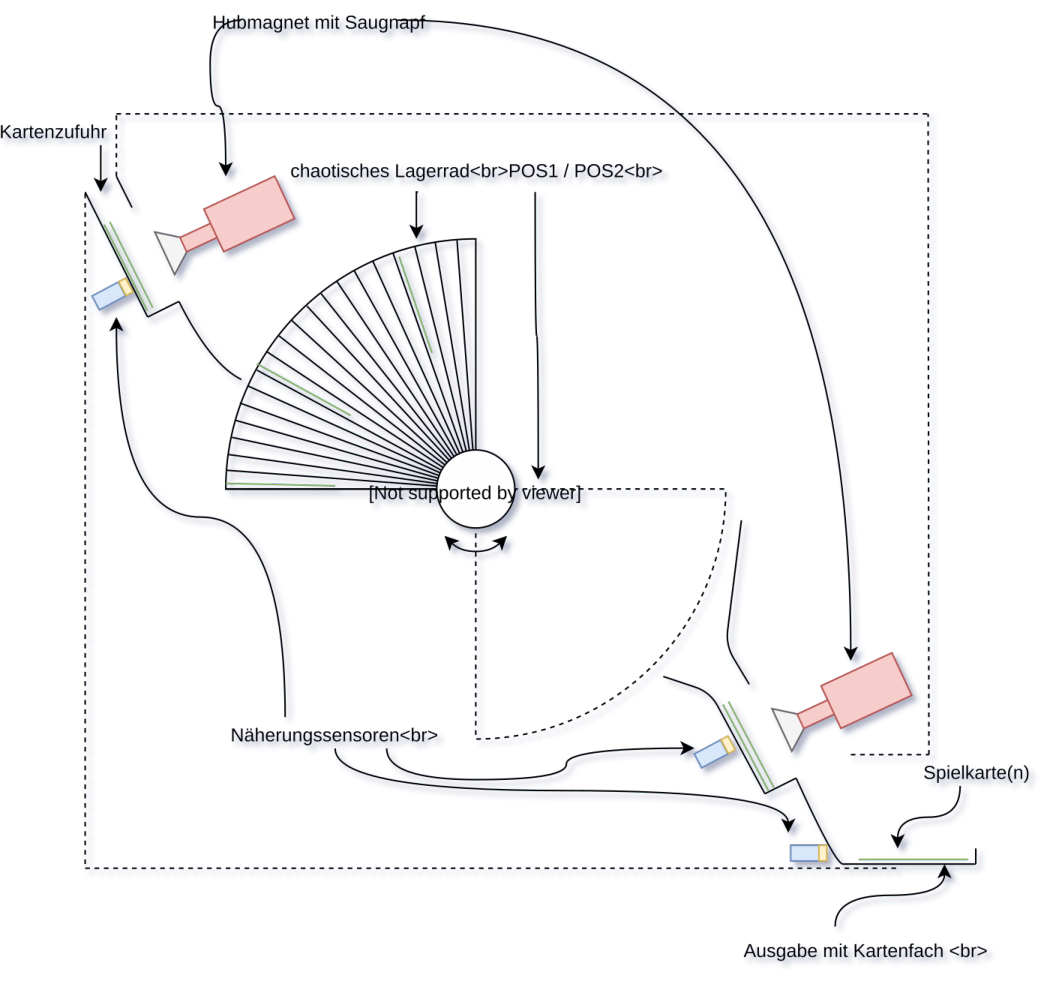
\includegraphics[width=0.6\textwidth]{fig/Reshuffled_Version_3_0_prinzip.pdf}
  \caption{Name des Bildes}
  \label{fig:verweis}
\end{figure}

Grundsätzlich basiert das Mischprinzip auf einer Art "Fächersystem".
Eingelegte Karten gelangen mithilfe eines ausgeklügelten Systems, welches aus einem Hubmagneten mit integriertem Saugnapf besteht, aus dem Einlegefach.
Erfolgt die Kartenentnahme, rutscht die Karte in ein zufälliges Fach des Lagerrads. Anschließend wird dieses Lagerrad in Drehbewegung versetzt um die gelagerten Karten auszugeben.

Der Benutzer steuert diese Maschiene mithilfe einer GUI welche auf einem 7" LCD Display angezeigt wird. Systemintern steuert ein 8-Bit Mikrocontroller der AVR-Familie den Ablauf.

\clearpage

\newpage
\thispagestyle{empty}
\mbox{}

\clearpage

\subsection*{Gender Erklärung}
\label{sec:gender-erklaerung}
Aus Gründen der besseren Lesbarkeit wird in dieser Arbeit die Sprachform des generischen Maskulinums angewendet. Es wird an dieser Stelle darauf hingewiesen, dass die ausschließliche Verwendung der männlichen Form geschlechtsunabhängig verstanden werden soll.

\subsection*{Über dieses Dokument}
\label{sec:ueber-dokument}
Diese Arbeit wurde in \LaTeX{} verfasst. Diese Art der Dokumentation bietet gegenüber den normalen Textverarbeitungen gewisse Vorteile hinsichtlich der Formatierung und des Einbindens von Grafiken. Auch Formeln können sehr einfach und effizient angegegeben werden. Die Rohfassung des Dokuments befindet sich auf dem Arnfelser Gitweb Server der HTBLA Kaindorf Abteilung Mechatronik.

\clearpage

\newpage
\thispagestyle{empty}
\mbox{}

\clearpage

\section*{Projektteam}
\label{sec:projektteam}

\subsection*{Stefan Hörmann}
\begin{wrapfigure}[10]{l}{0.5\textwidth}
\begin{center}
  \includegraphics[width=0.35\textwidth]{fig/logoMecha}
\end{center}
\end{wrapfigure}
\mbox{}\\
\mbox{}\\
\textbf{Aufgabenbereich}:\\
Mechanik\\
\textbf{Betreuer}:\\
Dr. Dipl-Ing. Gerhard Pretterhofer
\mbox{}\\
\mbox{}\\
\mbox{}\\
\mbox{}\\
\mbox{}\\
\mbox{}\\

\subsection*{Nicolas Perl}
\begin{wrapfigure}[10]{l}{0.5\textwidth}
\begin{center}
  \includegraphics[width=0.35\textwidth]{fig/logoMecha}
\end{center}
\end{wrapfigure}
\mbox{}\\
\mbox{}\\
\textbf{Aufgabenbereich}:\\
Elektronik\\
\textbf{Betreuer}:\\
Dipl-Ing. Manfred Steiner
\mbox{}\\
\mbox{}\\
\mbox{}\\
\mbox{}\\
\mbox{}\\

\subsection*{Alois Vollmaier}
\begin{wrapfigure}[10]{l}{0.5\textwidth}
\begin{center}
  \includegraphics[width=0.35\textwidth]{fig/logoMecha}
\end{center}
\end{wrapfigure}
\mbox{}\\
\mbox{}\\
\textbf{Aufgabenbereich}:\\
Informatik\\
\textbf{Betreuer}:\\
Dipl-Ing. Manfred Steiner
\mbox{}\\
\mbox{}\\
\mbox{}\\
\mbox{}\\
\mbox{}\\
\mbox{}\\
    \tableofcontents
    \mainmatter
    %\lohead{Hörmann Stefan}
\chapter{Mechanik}
\section{Einleitung}

\section{Anforderung}
\label{sec:Anforderung}
Die Arbeit des mechanischen Teiles besteht darin, eine Maschine,
die Spielkarten mischen und ausgeben kann zu entwerfen, zu konstruieren
und einen Teilaufbau durchzuführen. Die Maschine sollte in der Lage
sein 20 Spielkarten zu mischen und diese nach einem Spielmodus der
zuvor am LCD gewählt wurde auszugeben. Das Ziel ist es, die Spielkarten
optimal zu mischen, aber die Maschine dennoch kompakt und optisch
ansprechen zu entwerfen. Weiters sollte der Mischvorgang und die
Ausgabe der Karten nicht zu lange dauern. Die Teile der Maschine
sollten so konstruiert werden, dass sie kostengünstig produziert
werden können. Zum Schluss sollte noch ein Teilaufbau der Maschine
geschehen, um die Funktionalität der einzelnen Bereiche zu testen
und gegebenenfalls zu verbessern.

\section{Problemstellungen}
Ein Problem ist das begrenzte Budget unseres Teams, somit sind
wir auf gewisse Produktionsarten unserer Bauteile beschränkt.
Die Oberfläche der Karten ist ein
weiteres Problem, da diese sich nicht immer separieren lassen, dies
verursacht, dass oft zwei oder mehrere Karten auf einmal genommen
werden und das Konzept des optimalen Mischens zerstört.

\section{Konzepte}

\subsection{Anforderungen}

\begin{enumerate}
    \item \textbf{Kosten}  \\
    Der Automat sollte möglichst kostengünstig produziert werden,
    da das vorhandene Budget gering ist. Dies hat zur Folge, dass keine teuren Motoren
    oder ähnliche Bauteile zum Einsatz kommen können und keine teuren Bauteile produziert
    werden können.
    \item \textbf{Schnelligkeit} \\
    Um ein gutes Spielerlebnis zu garantieren, sollte der Automat keine
    lange Mischzeit aufweisen. Die Dauer, in der man die Karten einführt und auf den
    Mischen-Button klickt bis hin zur Ausgabe der ersten Karte sollte möglichst gering sein.
    \item \textbf{Mischgenauigkeit} \\
    Die Mischgenauigkeit ist die am schwersten gewichtete Anforderung,
    da es das Ziel ist ein optimales Mischen der Spielkarten zu erreichen, sollte
    diese Anforderung mit größter Priorität erfüllt werden.
    \item \textbf{Optik und Größe} \\
    Die Optik des Automaten soll schlicht gehalten werden. Der Automat sollte ein ansprechendes Design aufweisen und
    auf Messen und andere Ausstellungen präsentierbar sein. Der Automat
    sollte jedoch auch stabil konstruiert werden, muss aber dennoch mobil bleiben und
    darf eine gewisse Größe nicht Überschreiten.
\end{enumerate}

\subsection{Variantenvergleich}
Um alle oben angegebenen Anforderungen zu erfüllen, wurden mehrere Konzepte entworfen und diese verglichen.

\subsubsection{Variante 1 - Linearachsen}


\begin{figure}[hb]
    \centering
    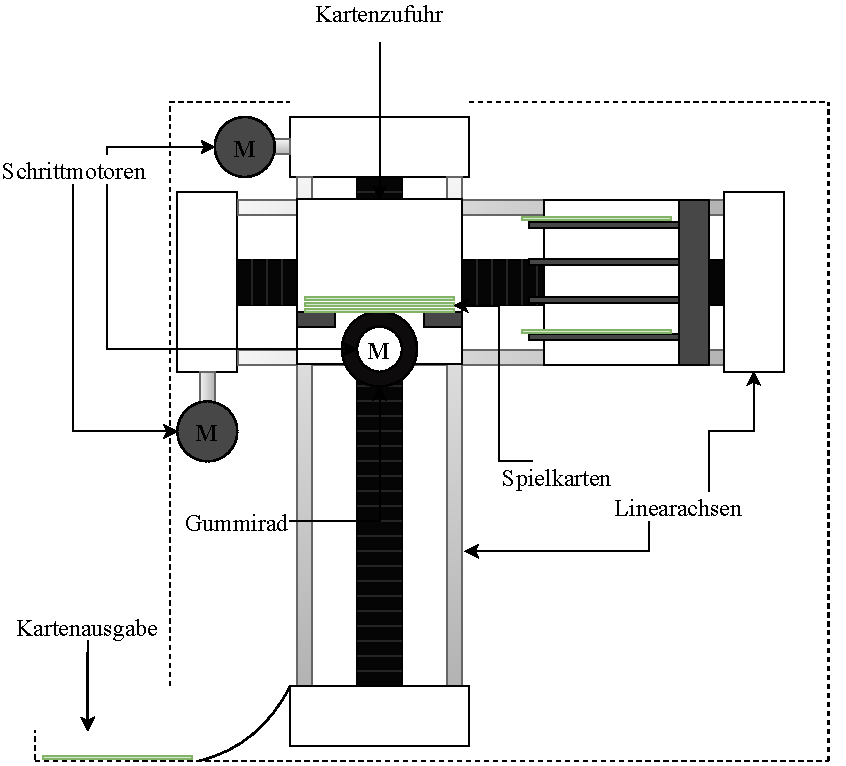
\includegraphics[scale=0.5,page=1]{fig/mech/Version1}
    \caption{Variante 1}
\end{figure}


Das erste Konzept würde mit zwei Linearachsen realisiert werden, diese wären im rechten Winkel zueinander
angeordnet. Die Senkrechte Linearachse ist mit einer Halterung versehen, diese Halterung ist in der Lage
ein Kartendeck aufzunehmen und die unterste Karte mithilfe eines Ausgaberades weiterzubefördern. Die zweite
Linearachse besitzt 4 Fächer, in der die Karten von der ersten Linearachsenausgabe zufällig befördert werden.
Dies wird realisiert, indem die erste Linearachse bei jeder Ausgabe zufällig das Fach durch hinauf und
hinabfahren wechselt. Befinden sich alle Karten im Lager, so fährt die erste Linearachse nach unten, danach
fährt die zweite Linearachse impulsiv nach links, um die Karten aus dem Lager zu befördern. Diese fallen
Senkrecht in das Lager der ersten Linearachse, wo sie nun zum Ausgeben durch das Ausgaberad bereitliegen. \\



Durch die schnelle Bewegung der Linearachsen ist es möglich einen schnellen Mischprozess zu erreichen,
auch die Tatsache das es nur ein rotierendes Rad gibt und zwei Bewegliche Linearachsen führt dazu, das
Fehler bei Bewegungen nur selten Auftreten. Jedoch besteht durch den hohen Aufbau der Maschine und durch die hohe
Position der zweiten Linearachse die sich horizontal bewegt die Gefahr des Umkippens der Maschine, und somit ist
keine Stabilität mehr gegeben. Der Preis der Linearachsen ist ein weiterer Nachteil dieses Konzeptes, eine Linearachse
die unsere Anforderungen entspricht, wäre mit Motor und Schlitten zu teuer für unser Budget. \\

\textbf{Vorteile:}
\begin{itemize}
    \item schnelles Mischen
    \item wenige Fehlerquellen
\end{itemize}
\textbf{Nachteile:}
\begin{itemize}
    \item teuer
    \item großer Aufbau %Genaueres Beschreiben der Vor und Nachteile?
    \item instabil
\end{itemize}

\subsubsection{Variante 2 - Lagerrad mit Asugaberäder}

\begin{figure}[hb]
    \centering
    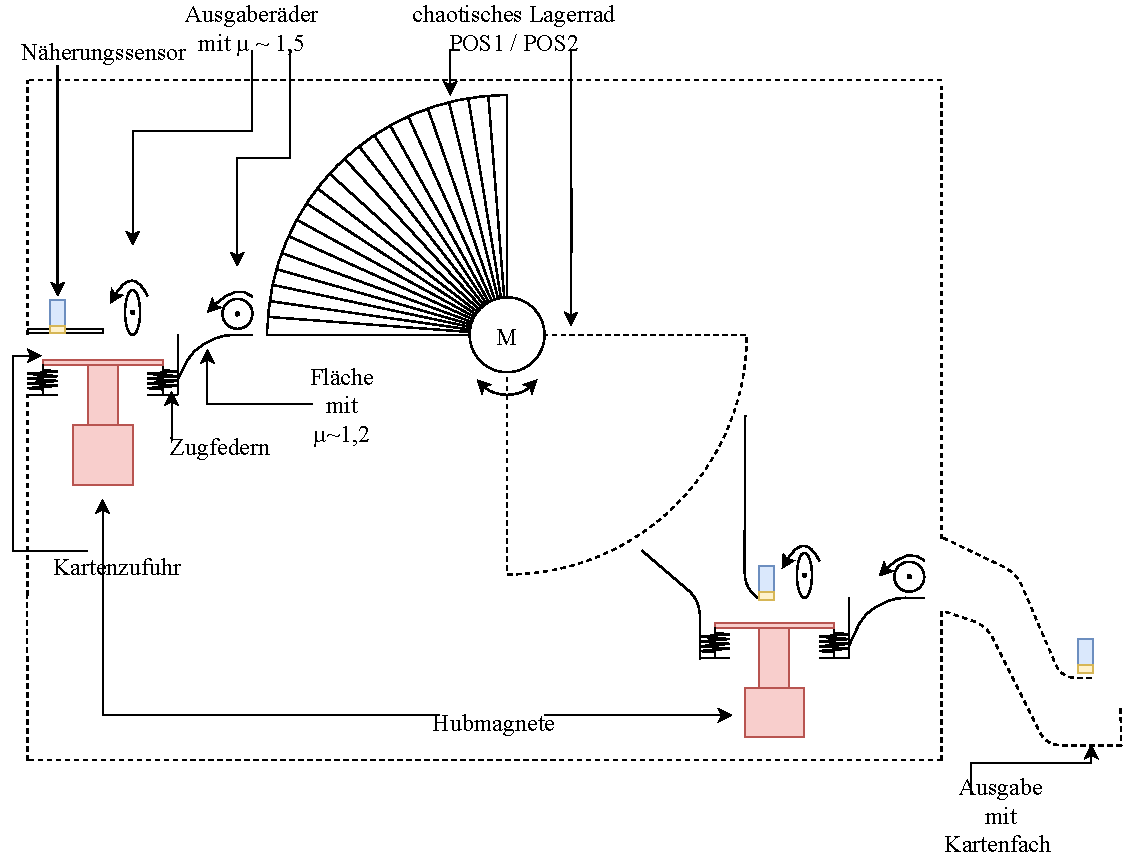
\includegraphics[scale=0.5,page=1]{fig/mech/Version2}
    \caption{Variante 2}
\end{figure}

Beim zweiten Konzept wird als Lager ein Viertel eines Zylinders benutzt. In diesem befinden
sich verschiedene Fächer, in der die Karten eingelagert werden. Dieser wird mit einem Motor betrieben
und dreht sich somit in die vorgegebenen Positionen um das Einlagern und das Ausgeben der Karten zu ermöglichen.
Die Karteneingabe erfolgt über einen Schlitz in der Frontplatte der Maschine, dort befindet sich ein Hubmagnet, der die Karten
zum weiterbefördern nach oben drückt. Ein Kapazitiver Sensor sorgt dafür, das sichergestellt werden kann, dass sich Karten auf dem Hubmagnet befinden.
Um eine Karte in das Lager zu befördern wird der Hubmagnet eingeschaltet und drückt das Kartendeck auf das erste Ausgaberad, um die Kraft des Hubmagnetes zu minimieren sind Zugfedern angebracht.
Das Ausgaberad befördert eine Karte weiter vor zum zweiten Ausgaberad, welches wiederum sicherstellt, das nur eine Karte in das Lagerrad transportiert wird.
Danach dreht das Lagerrad auf eine andere zufällig ausgewählte Position. Dieser Prozess wird so lange wiederholt, bis alle Karten des Kartendecks sich im Lagerrad befinden.
Befinden sich alle Karten im Lagerrad, so dreht sich dieses mit einer hohen Geschwindigkeit und wirft somit die Karten auf der Hinterseite der Maschine in eine Auffangführung. %Ist Geschwindigkeit der richtige Begriff? Eher Moment oder Drehzahl?
Diese Auffangsführung befördert die Karten in einen gleichen Mechanismus wie bei der Vorderseite der Maschine, in der sie von einem Hubmagneten nach oben gedrückt werden und von zwei Ausgaberädern zur
Kartenentnahme geschoben werden. Da die Karten zum Schluss nach einem Spielmodus und somit in einer bestimmten Anzahl ausgegeben werden, befindet sich ein Kapazitiver Sensor auch bei der Ausgabe der Karten,
dieser soll überprüfen, ob die Karten von dem Spieler bereits genommen wurden oder nicht.\\

Durch den niedrigen Aufbau der durch ein "Fließbandartiges" befördern der Karten erreicht wird, besitzt die Maschine ein hohes Maß an Stabilität, jedoch entsteht dadurch auch der Nachteil, dass die Maschine sehr lang wird. Da dieses
Konzept 5 bewegliche Räder besitzt, sowie zwei Hubmagneten, ist es anfällig für Fehler beim Bewegungsablauf. Auch kann nicht garantiert werden, dass nur eine Karte in das Lagerrad befördert wird, dies würde das Konzept des optimalen
Mischens zerstören. Die vielen Bauteile führen auch zu teureren Anschaffungskosten, die wir stark vermeiden möchten.\\

\textbf{Vorteile:}
\begin{itemize}
    \item stabil
    \item niedriger Aufbau
\end{itemize}
\textbf{Nachteile:}
\begin{itemize}
    \item lange Gesamtgröße
    \item viele bewegliche Bauteile / Fehlerquellen
\end{itemize}

\subsubsection{Variante 3 - Lagerrad mit Saugnäpfe}

\begin{figure}[H]
    \centering
    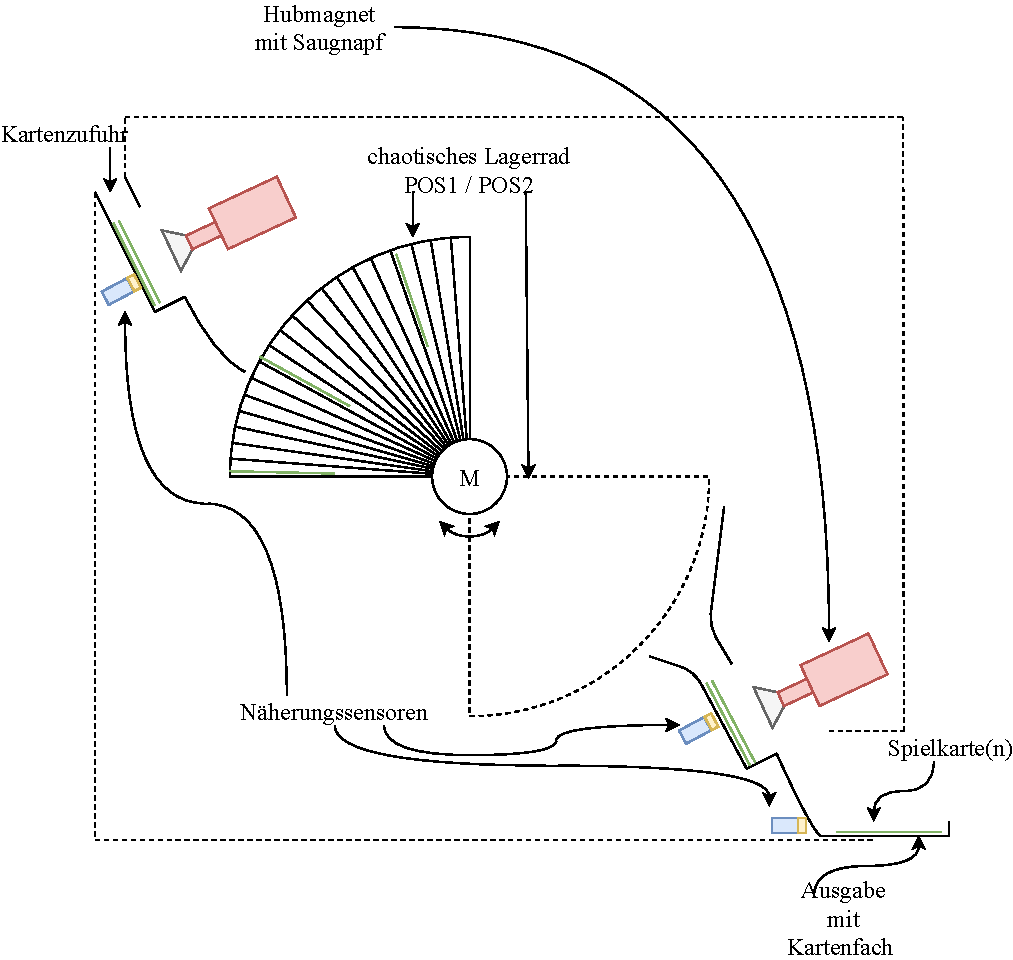
\includegraphics[scale=0.5,page=1]{fig/mech/Version3}
    \caption{Variante 3}
\end{figure}

Das dritte Konzept besitzt ein identes Lagersystem wie das zweite Konzept, ein Lagerrad, das in Fächer unterteilt ist und über einen Motor diverse Positionen einnehmen kann.
Das Kartendeck wird in den oberen / vorderen Anfang der Maschine eingeführt. Dort liegt, es schräg in einem Winkel von ca. 60°. Um sicherzustellen, dass sich Karten in dieser Halterung befinden
ist ein Kapazitiver Sensor an der Unterseite angebracht. Ein Hubmagnet der im rechten Winkel zu den Karten über der Halterung angebracht ist, saugt jede Karte einzeln an, indem ein Saugnapf, der an einem Hubmagneten
befestigt, ist heruntergedrückt wird. Ist die Karte angesaugt, so wird der Hubmagnet von einer Feder in seine Ausgangsstellung zurückgebracht, dabei wird die Spielkarte durch eine Platte abgestreift und fliegt somit in das Lager des
Lagerrades hinein. Dieser Prozess wird so lange wiederholt, bis sich alle Spielkarten des Kartendecks im Lagerrad befinden. Sind alle Karten im Lagerrad, so dreht sich dieses und wirft die Karten auf der Rückseite der Maschine in eine Führung, die die Karten in eine zweite Halterung befördern. Diese zweite Halterung ist ident aufgebaut wie die erste. Die Karten werden nun wieder einzeln vom Saugnapf angesaugt und in ein Ausgabefach am Ende der Maschine befördert. Im Ausgabefach befindet sich
ein Kapazitiver Sensor, dieser überprüft, ob die Karten vom Spieler bereits genommen wurden oder nicht.\\

Durch die wenigen Bauteile die dieses Konzept besitzt, nämlich zwei Hubmagnete und einen Motor, ist das Konzept wenig fehleranfällig bei Bewegungsabläufe. Außerdem ist es
durch die wenigen Bauteile im Vergleich billiger als die anderen Konzepte. Ein Problem dieses Konzeptes ist seine Höhe und dass das Lagerrad sich in der Mitte der Maschine befindet,
jedoch ist durch das geringe Gewicht des Lagerrades noch immer genügend Stabilität vorhanden, auch wenn sich dieses mit voller Geschwindigkeit dreht. \\

\textbf{Vorteile:}
\begin{itemize}
    \item billig
    \item wenig bewegliche Bauteile
\end{itemize}
\textbf{Nachteile:}
\begin{itemize}
    \item hocher Aufbau
\end{itemize}

 \subsection{Ausgaberäder}
Um die Karten weiterzubefördern werden bei zwei Konzepten Ausgaberäder benutzt, für diese gibt es verschiedene Konzepte dies sich in Preis, Herstellung und Funktionalität unterscheiden.\\
Das Ausgaberad ist mit einem Motor verbunden, dieses sorgt dafür das eine Karte von einem Kartendeck weiterbefördert wird.
\begin{itemize}
    \item \textbf{Rundes Ausgaberad}
\end{itemize}

\begin{figure}[H]
    \centering
    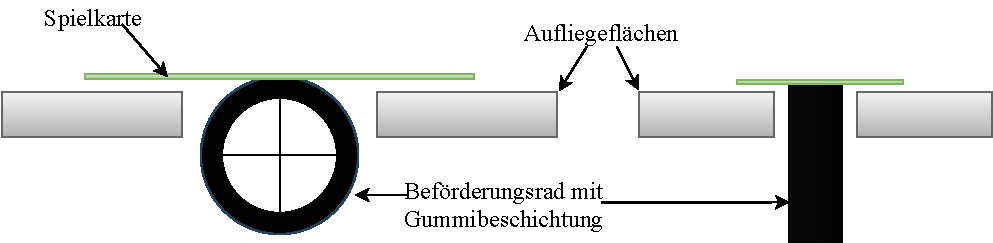
\includegraphics[scale=0.5,page=1]{fig/mech/RundesAusgaberad-Page-1}
    \caption{Rundes Ausgaberad}
\end{figure}

    Die einfachste Möglichkeit dieses Rad zu entwerfen, wäre ein einfaches rundes Ausgaberad. Dieses Rad wäre mit einer Schicht umhüllt, welche die Reibung
        dem Rad und der Karte erhöht. Das runde Rad wäre einfach zu fertigen und würde somit wenig kosten und nur einen geringen Zeitaufwand haben. Jedoch
        ist das Rad in der Lage mehr als nur eine Karte mit sich mitzuziehen, da es durchgehen Kontakt mit der Spielkartenoberfläche hat, dies hätte zur
        Folge, das mehrere Spielkarten zugleich weiterbefördert werden.
\begin{itemize}
    \item \textbf{Eliptisches Ausgaberad}
\end{itemize}

\begin{figure}[H]
    \centering
    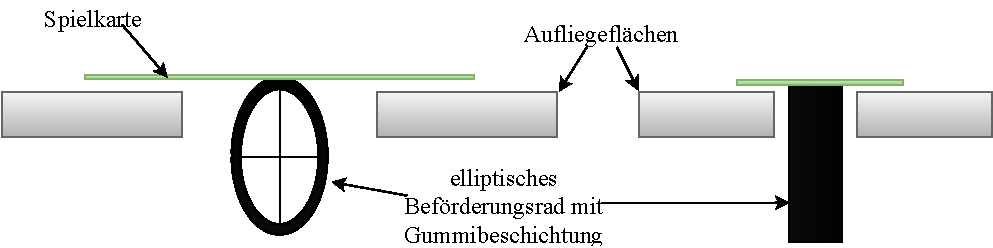
\includegraphics[scale=0.5,page=1]{fig/mech/ElliptischesAusgaberad}
    \caption{Eliptisches Ausgaberad}
\end{figure}


Ein elliptisches Ausgaberad wäre das nächste Konzept, dieses Rad wird auch wie beim ersten Rad mit einem Motor verbunden, um somit Karten zu befördern.
Durch die elliptische Form des Rades herrscht kein durchgehender Kontakt mit der Oberfläche der Spielkarte, aus diesem Grund ist die Chance das mehrere
Karten zugleich befördert werden minimiert. Jedoch setzt dies auch einen Motor voraus der in kurzer Zeit ein hohes Drehmoment entwickelt, da die
Karten schlagartig befördert werden. Das elliptische Rad würde in der Produktion auch mehr Kosten verursachen und wäre Zeitintensiver in der Herstellung. \\

\begin{itemize}
    \item \textbf{Vergleich der Ausgaberäder}
\end{itemize}

Da das primäre Ziel unserer Arbeit das perfekte Mischen der Spielkarten ist, wäre es besser das elliptische Ausgaberad in Betracht zu ziehen. Die Kosten
die durch die aufwendigere Herstellung entstehen wären überschaulich und somit wäre es von Vorteil dieses Konzept zu wählen. Durch die Tatsache, dass das elliptische Rad
das Kartendeck nur jede halbe Umdrehung berührt und nicht konstant, muss ein Motor für die Räder eingesetzt werden, der sich schnell genug dreht, um eine Karte mit einer Berührung
des Rades "herauszuschießen". Dies würde aber keine zusätzlichen Kosten verursachen. Aus diesen Gründen fällt die Wahl auf das \textbf{elliptisches Ausgaberad}. \\

\subsection{Klemmmechanissmen}
Um beim Ausgeben und beim Weiterbefördern der Karten die Chance zu minimieren das mehrere Karten auf einmal weiterbefördert werden, wird ein
Klemmmechanismus benutzt, dieser sorgt dafür das die Karten von außen Geklemmt werden, und somit nur die unterste Karte durch das Drehen des
Ausgaberades weiterbefördert wird.

\begin{itemize}
    \item \textbf{Primitiver Klemmmechanissmus}
\end{itemize}

\begin{figure}[H]
    \centering
    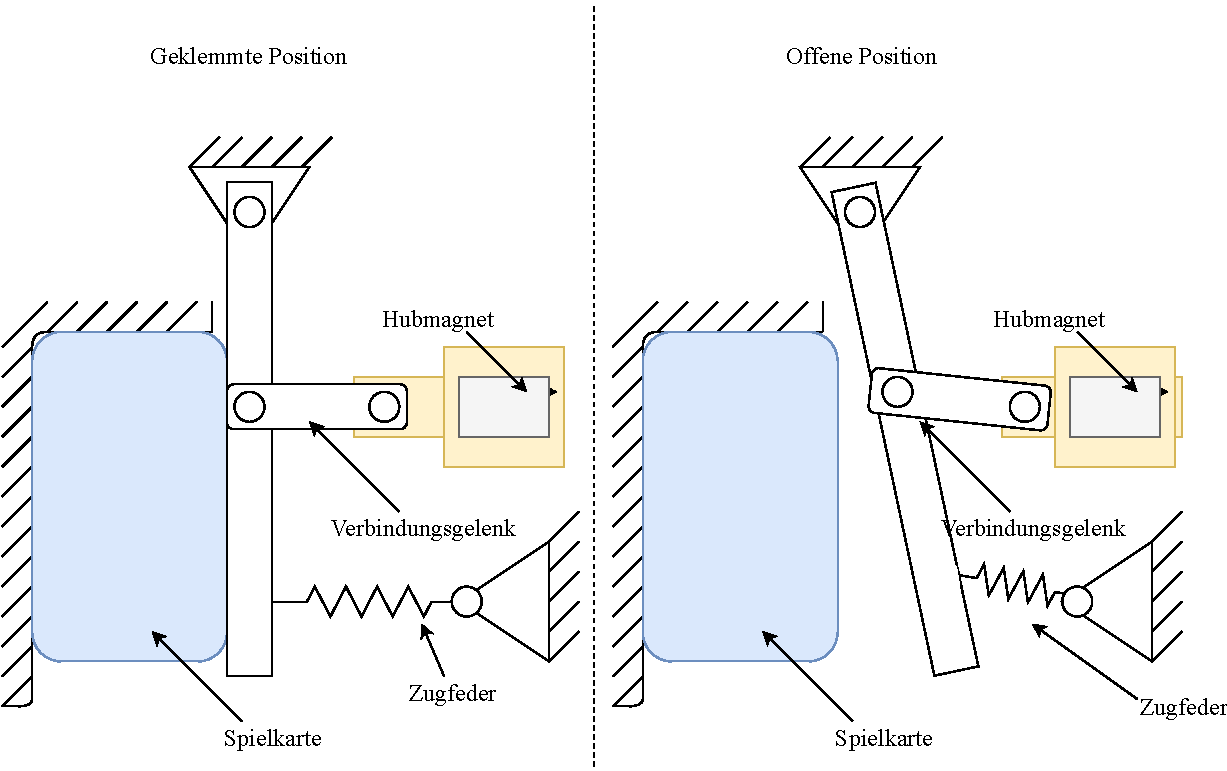
\includegraphics[scale=0.5,page=1]{fig/mech/Klemmmechanissmus1}
    \caption{Primitiver Klemmmechanissmus}
\end{figure}

Dieser Klemmmechanismus ist der primitivste und einfachste, dadurch aber auch der billigste. Die Karten werden auf der einen Seite an eine feste Wand gedrückt
auf der anderen Seite werden sie durch ein bewegliches Gelenk fixiert. Dieses Gelenk wird durch das Einschalten des Hubmagneten in die geschlossene Position bewegt,
soll das Gelenk wieder öffnen, so wird der Hubmagnet ausgeschaltet und eine Zugfeder zieht das Gelenk wieder in seine Ausgangsposition zurück.

\begin{itemize}
    \item \textbf{Komplexer Klemmmechanissmus}
\end{itemize}

\begin{figure}[H]
    \centering
    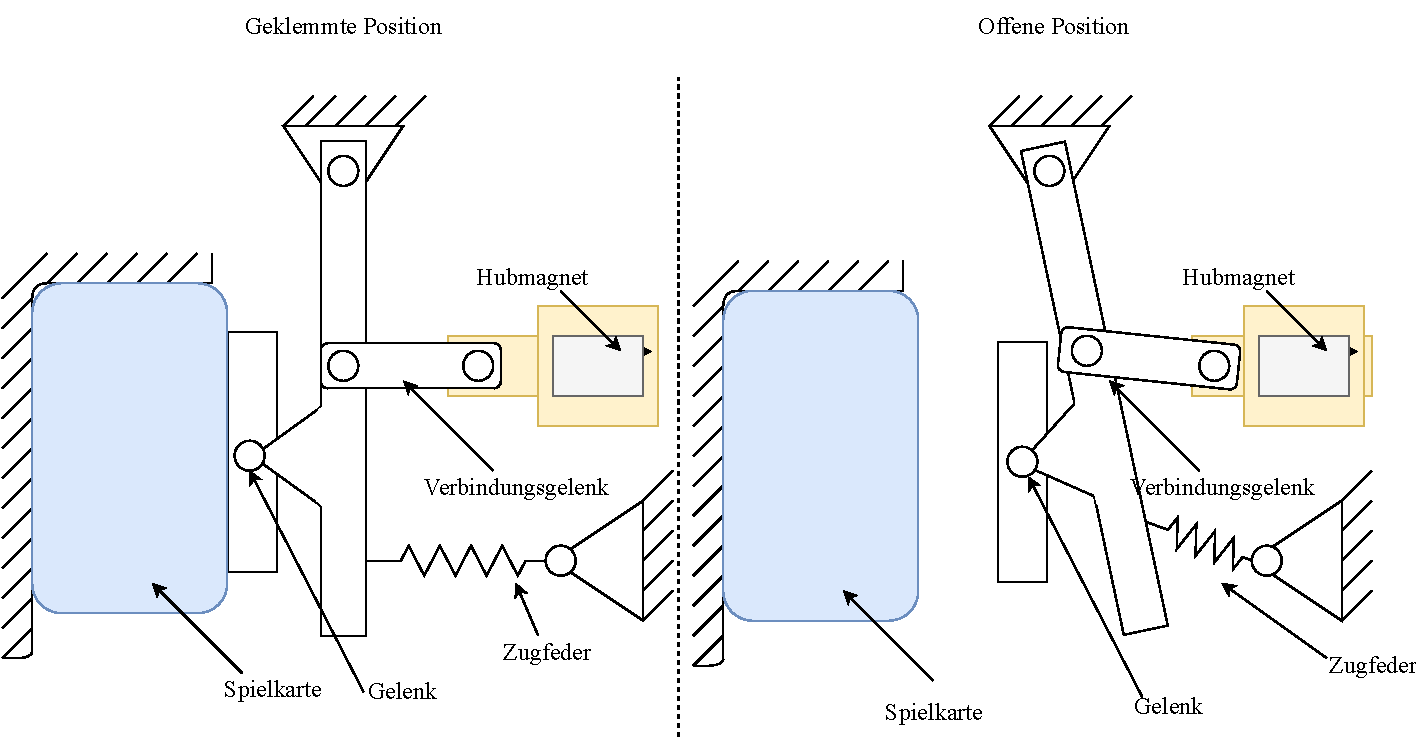
\includegraphics[scale=0.5,page=1]{fig/mech/Klemmmechanissmus2}
    \caption{Komplexer Klemmmechanissmus}
\end{figure}

Bei diesem Mechanismus werden die Karten auf der einen Seite durch eine feste Wand geklemmt, auf der anderen werden sie durch ein Gelenk geklemmt, dieses Gelenk
ist beweglich und gleicht somit verschiedene Kartengrößen aus. Um das Gelenk dieses Konzeptes zu schließen wird ein Hubmagnet benötigt, wird dieser eingeschalten
so schließt das Gelenk und passt sich der Kartengröße an. Soll es wieder geöffnet werden, so wird der Hubmagnet ausgeschaltet und eine Zugfeder bringt den Mechanismus wieder in den
Grundzustand. Dieses Konzept ist aufwendiger zu realisieren wie das erste, jedoch kann es verschiedene Kartengrößen klemmen und gleicht sich den Karten an. Das Konzept ist
dafür aber auch aufwendiger in der Produktion.

\begin{itemize}
    \item \textbf{Gummi Klemmmechanissmus}
\end{itemize}

\begin{figure}[H]
    \centering
    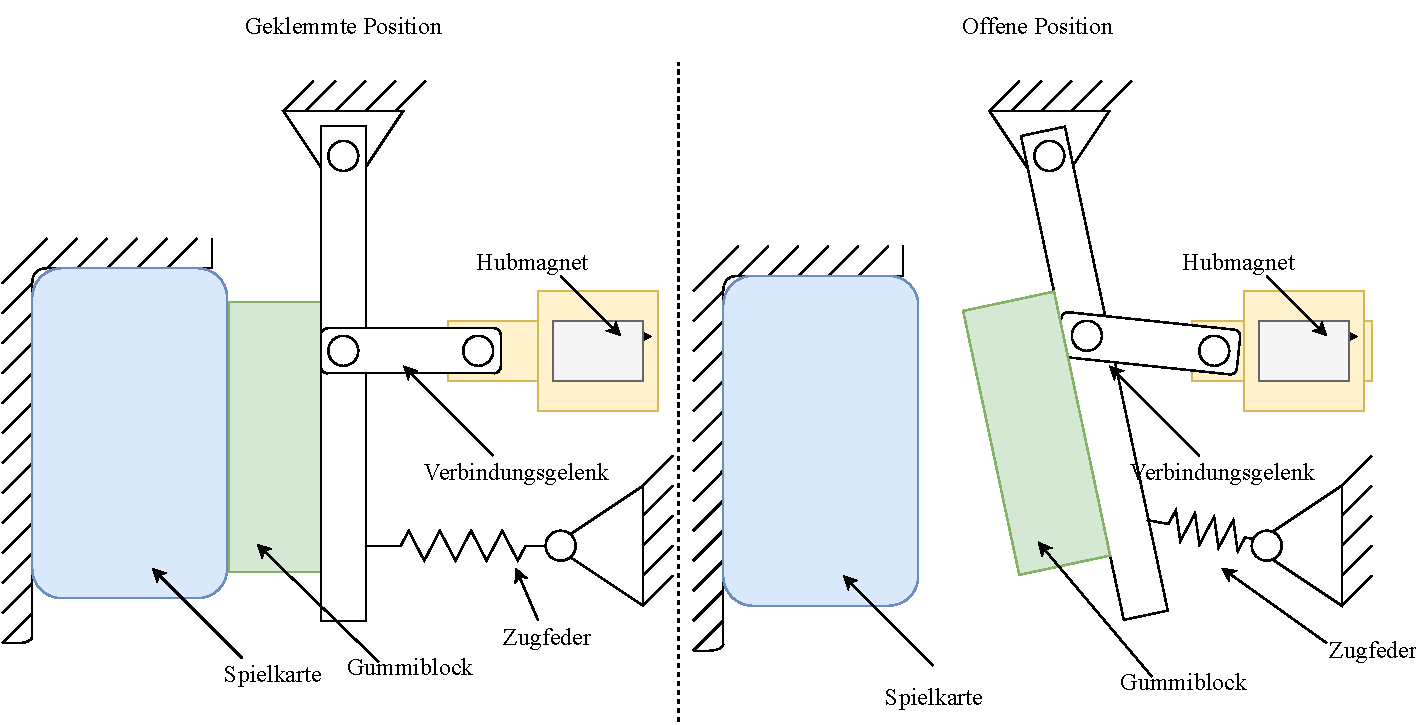
\includegraphics[scale=0.5,page=1]{fig/mech/Klemmmechanissmus3}
    \caption{Gummi Klemmmechanissmus}
\end{figure}

Der letzte Mechanismus ist funktionsmäßig gleich wie der primitive Klemmmechanismus, der einzige Unterschied besteht aus dem
Gummi-ähnlichen Block, der auf der Klemmfläche sitzt. Dieser soll sich den Karten anpassen und sorgt dafür das alle Karten gleichmäßig
geklemmt werden, auch erhöht es die Reibung zwischen den Karten und der Klemmoberfläche. Dieses Konzept wäre in der Herstellung vergleichsweise
einfach zu realisieren und dadurch auch billig in der Herstellung.


\begin{itemize}
    \item \textbf{Vergleich der Klemmmechanissmen}
\end{itemize}

Da alle Mechanismen die gleiche Anzahl an Bauteile erfordern, spielt der Preis bei dieser Auswahl keine große Rolle. Aus diesem Grund
sind die Kriterien Funktionalität und Aufwand in der Produktion. Der erst Mechanismus wäre der einfachste in der Produktion, jedoch
hat er durch sein nicht anpassungsfähiges Klemmgelenk Probleme mit verschiedenen Kartengrößen, aus diesem Grund fällt er bei diesem Auswahlverfahren durch.
Der zweite Mechanismus wäre der komplexe Klemmmechanismus, dieser würde sich zwar verschiedenen Kartengrößen anpassen, wäre aber etwas aufwendiger in der
Produktion und ist somit auch nicht die bevorzugte Wahl. Da er einfach in der Produktion ist und sich verschiedenen Kartengrößen anpassen kann, fällt die Wahl jedoch auf den Gummiklemmmechanismus.

\subsection{Seperation der Karten}
Da bei "Variante 3 - Lagerrad mit Saugnäpfe" Saugnäpfe mit Unterdruckprinzip in Verwendung kommen würden, liegt das Problem vor,
dass die Karten aneinander haften, dieses Problem entsteht durch den Unterdruck der beim Aufpressen des Saugnapfes entsteht.
Um zu garantieren, das nur eine Karte in das Lager befördert wird oder ausgegeben wird, müssen diese aneinander
haftende Karten getrennt werden.

\begin{itemize}
    \item \textbf{Selbständiges Loslösen der Karten}
\end{itemize}

Die billigste und primitivste Möglichkeit die Karten zu separieren wäre abzuwarten bis Luft zwischen den Karten von außen eindringt und alle Karten sich durch die Schwerkraft
von der eigentlich angesaugten Karte getrennt haben. Jedoch zeigten Versuche die durchgeführt wurden, dass dies zu lange
dauern würde und das Spielerlebnis somit beeinflussen würde.

% Please add the following required packages to your document preamble:
% \usepackage{multirow}
\begin{table}[H]
    \centering
\scalebox{0.8}{
    \begin{tabular}{|c|c|c|c|c|c|c|c|}
        \hline
        \textbf{}                         & \multicolumn{7}{c|}{\textbf{Sekunden}}                                                                  \\ \hline
        \multirow{21}{*}{\textbf{Karten}} &    & 1. Durchgang & 2. Durchgang & 3. Durchgang & 4. Durchgang & 5. Durchgang        & Mittelwert       \\ \cline{2-8}
        & 20 & 9.69         & 9.32         & 8.92         & 8.54         & 4.53                & 8.2              \\ \cline{2-8}
        & 19 & 9.1          & 9.97         & 13.82        & 6.71         & 7.75                & 9.47             \\ \cline{2-8}
        & 18 & 15.39        & 8.93         & 6.51         & 13.05        & 15.25               & 11.826           \\ \cline{2-8}
        & 17 & 6.45         & 6.67         & 6.16         & 8.06         & 6.97                & 6.862            \\ \cline{2-8}
        & 16 & 10.76        & 6.52         & 10.62        & 11.37        & 6.97                & 9.248            \\ \cline{2-8}
        & 15 & 12.81        & 6.45         & 16.22        & 8.74         & 4.7                 & 9.784            \\ \cline{2-8}
        & 14 & 3.46         & 9.78         & 11.72        & 5.85         & 6.39                & 7.44             \\ \cline{2-8}
        & 13 & 4.85         & 8.18         & 10.77        & 10.5         & 3.43                & 7.546            \\ \cline{2-8}
        & 12 & 15.1         & 5.37         & 12.36        & 8.54         & 12.31               & 10.736           \\ \cline{2-8}
        & 11 & 15.83        & 6.32         & 5.58         & 5.08         & 1.12                & 6.786            \\ \cline{2-8}
        & 10 & 7.14         & 8.4          & 11.21        & 12.76        & 4.43                & 8.788            \\ \cline{2-8}
        & 9  & 7.48         & 6.24         & 11.87        & 4.32         & 6.36                & 7.254            \\ \cline{2-8}
        & 8  & 4.68         & 5.65         & 8.61         & 5.2          & 4.41                & 5.71             \\ \cline{2-8}
        & 7  & 9.73         & 8.29         & 9.13         & 5.35         & 11.2                & 8.74             \\ \cline{2-8}
        & 6  & 5.41         & 5.16         & 8.05         & 4.98         & 9.73                & 6.666            \\ \cline{2-8}
        & 5  & 6.06         & 4.81         & 7.8          & 4.73         & 7.19                & 6.118            \\ \cline{2-8}
        & 4  & 4.86         & 9.87         & 7.74         & 9.51         & 7.4                 & 7.876            \\ \cline{2-8}
        & 3  & 4.54         & 11.31        & 4.31         & 6.74         & 10.82               & 7.544            \\ \cline{2-8}
        & 2  & 4.83         & 2.19         & 4.13         & 3.78         & 5.71                & 4.128            \\ \cline{2-8}
        &    &              &              &              &              & \multicolumn{2}{c|}{Mittelwert: 7.932} \\ \hline
    \end{tabular}}
    \caption{Tabelle Haftzeit der Karten}
    \label{tab:my-table}
\end{table}

\begin{figure}[H]
    \centering
    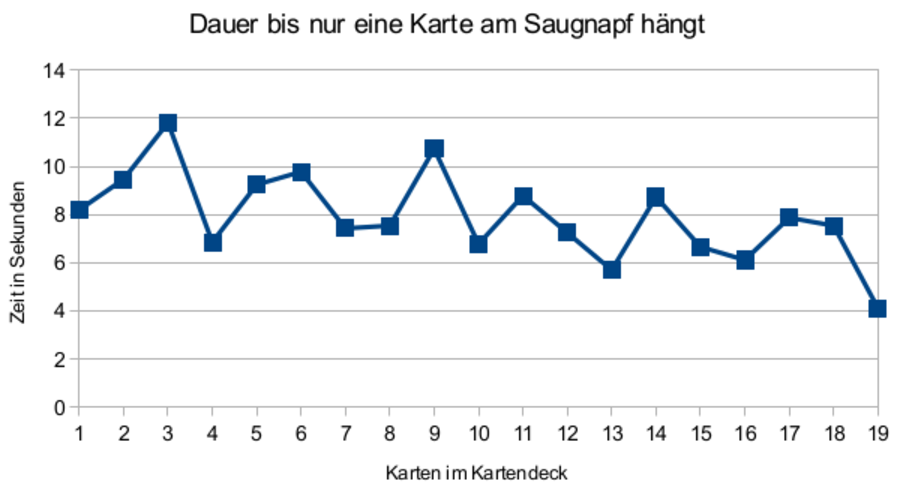
\includegraphics[scale=1,page=1]{fig/mech/Haftzeit}
    \caption{Diagramm Haftzeit der Karten}
\end{figure}

Wie man in Tabelle 1.1 und in Abbildung 1.9 erkennen kann dauert es im Durchschnitt 7,932 Sekunden bis sich nur mehr die
eigentlich angesaugte Karte am Saugnapf befindet. Der Versuch wurde mit 1Kg Ansaugdruck durchgeführt. Es gab insgesamt
5 Durchgänge, auch wurden alle Möglichkeiten der Kartenanzahl im Kartendeck berücksichtigt, so saugte der Saugnapf
bei der ersten Durchgangsreihe die erste Karte an, die auf 19 anderen Karten liegt, bis hin zu einem Saugnapf, der
eine Karte ansaugt, die nur auf einer einzelnen anderen Karte liegt.

\textbf{Vorteile:}
\begin{itemize}
    \item billig
    \item keine zusätzlichen Bauteile benötigt
\end{itemize}
\textbf{Nachteile:}
\begin{itemize}
    \item lange Wartezeit
    \item unzuverlässig
\end{itemize}

\begin{itemize}
    \item \textbf{Rütteln}
\end{itemize}
Ein weiteres Konzept um die angesaugte Karten von den anderen zu trennen wäre die Karten minimal zu rütteln.
Da die angesaugte Karte viel stärken an dem Saugnapf haftet als die Karten, die nur an der angesaugten Karten haften,
könnte der Hubmagnet oder der Ansaugmechanismus leicht gerüttelt werden, so würden die anderen Karten schneller den
Unterdruck untereinander verlieren und sich somit schon in kurzer Zeit separieren lassen. Jedoch müsste für dieses Konzept
ein Mechanismus entwickelt und produziert werden der nur einen ausgewählten Bereich rüttelt, dies wäre mit weiteren Bauteilkosten und
Aufwand verbunden.

\textbf{Vorteile:}
\begin{itemize}
    \item zuverlässig
\end{itemize}
\textbf{Nachteile:}
\begin{itemize}
    \item teurer
    \item zusätzliche Bauteile
    \item zusätzliche Größe
\end{itemize}


\begin{itemize}
    \item \textbf{Abstreifbürsten}
\end{itemize}

Bei diesem Konzept sind bürstenartige Abstreifvorrichtungen in der Kartenhalterung angebracht. Diese Bürsten sollen beim Aufheben der
angesaugten Karte die anderen Karten die mitgehoben wurden abstreifen. Dabei ist es wichtig, dass die Bürste den richtigen Widerstand aufbringt.
Ist der Widerstand zu hoch, wird auch die eigentlich angesaugt Karte mit abgestreift, ist er jedoch zu niedrig ist es möglich, dass die anderen Karten
die mitgehoben werden nicht abgestreift werden.

\textbf{Vorteile:}
\begin{itemize}
    \item zuverlässig
    \item billig
\end{itemize}
\textbf{Nachteile:}
\begin{itemize}
    \item Karten werden seitlich abgenützt
    \item komplizierter Einbau
\end{itemize}

\begin{figure}[H]
    \centering
    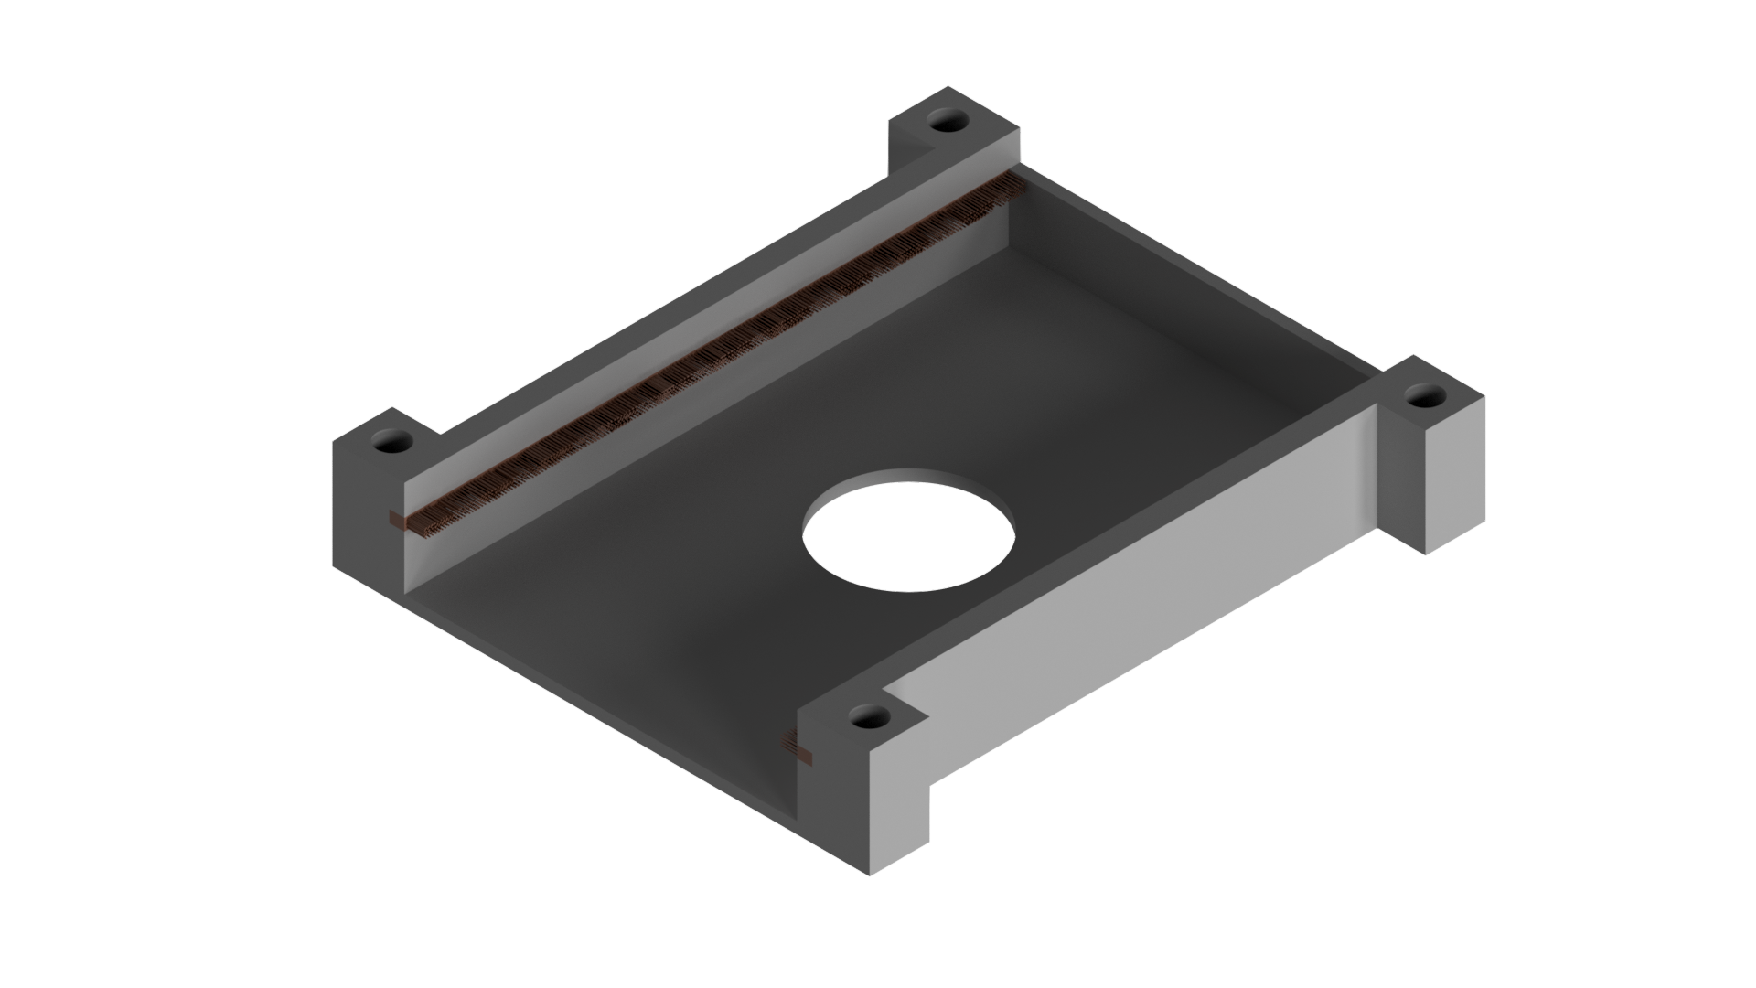
\includegraphics[scale=0.5,page=1]{fig/mech/AusgabeMitBuersten}
    \caption{Ausgabe mit Bürsten}
\end{figure}

\begin{itemize}
    \item \textbf{Gummiabsstreifer}
\end{itemize}

Dieses Konzept funktioniert ähnlich wie das "Abstreifbürsten Konzept". Es besitzt seitlich Abstreifplatten die aus Gummi sind, diese
sollen der angesaugten Karte helfen, die mitgezogenen Karten abzustreifen. Wie beim vorherigen Konzept muss hierbei das Gummi auch so
dimensioniert werden, dass es einerseits nicht zu steif ist und die eigentlich angesaugt Karte abstreift, andererseits sollte es steif genug sein, um die Karten die mitgehoben werden abzustreifen. Man die Steifigkeit des Gummistreifens verändern, indem man die Breite der Einschnitte
erhöht oder vermindert.

\begin{figure}[H]
    \centering
    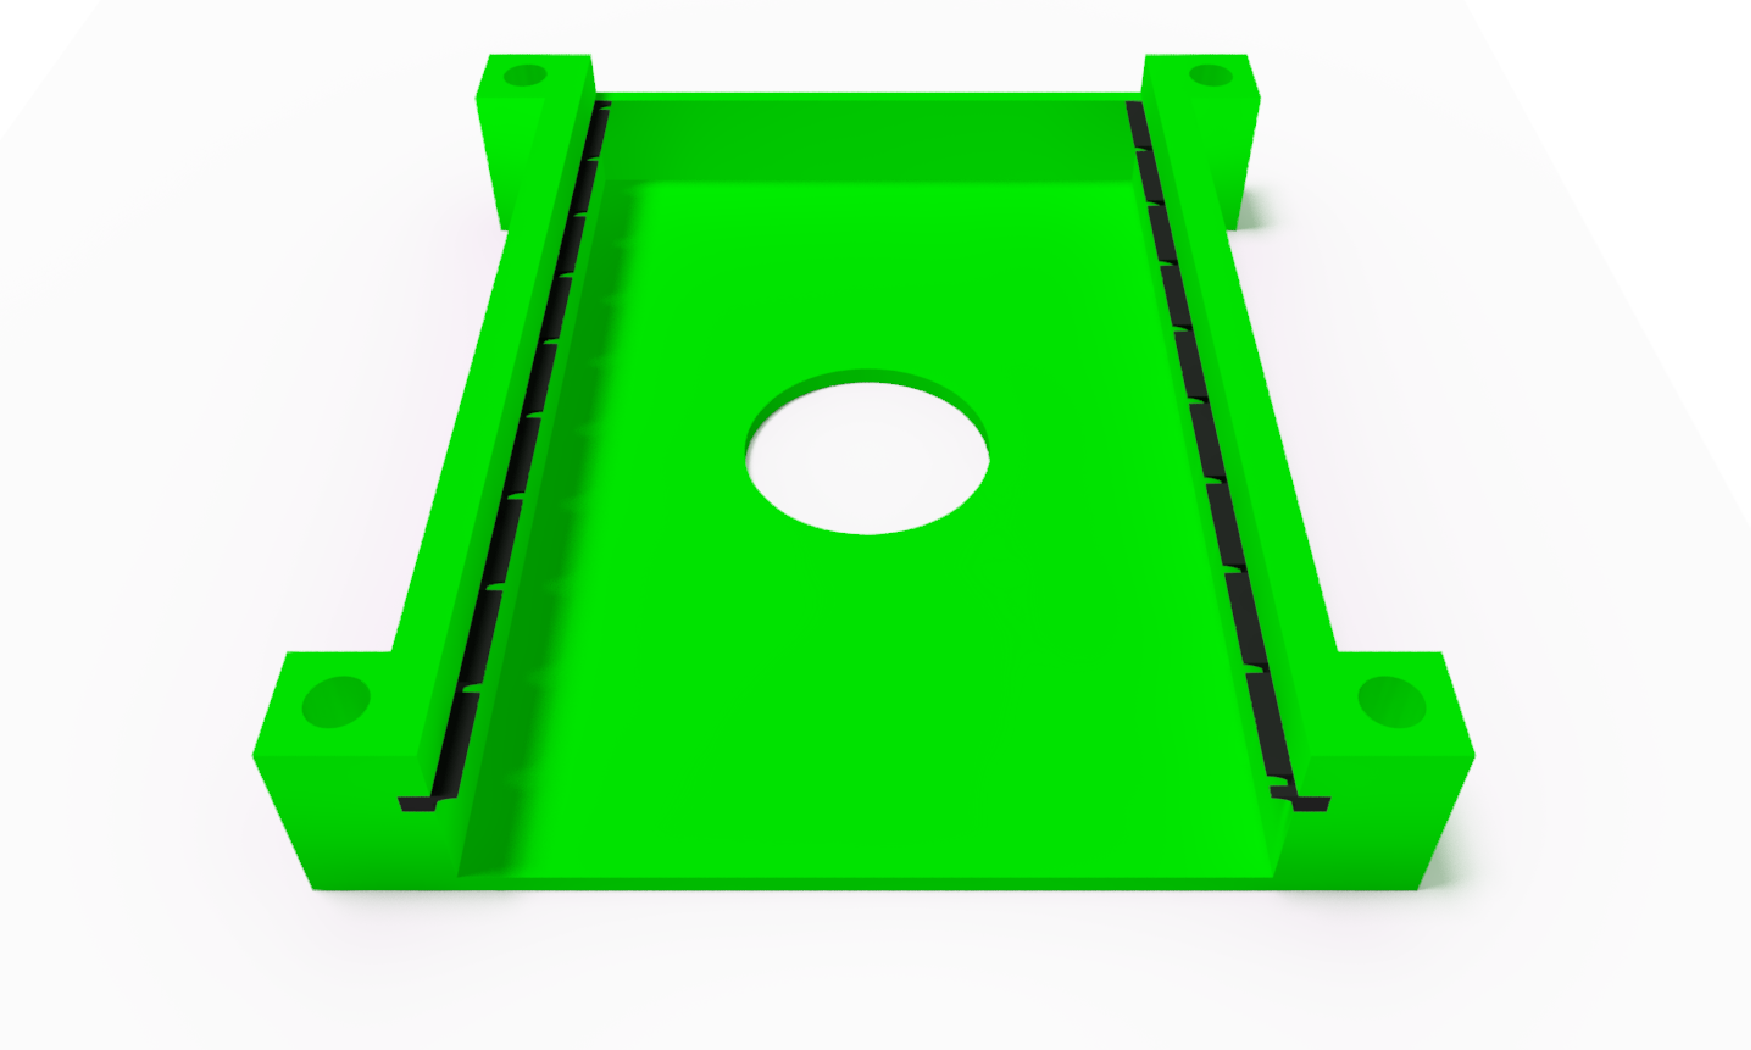
\includegraphics[scale=0.5,page=1]{fig/mech/AusgabeMitGummiabstreifer}
    \caption{Ausgabe mit Bürsten}
\end{figure}

\textbf{Vorteile:}
\begin{itemize}
    \item zuverlässig
    \item billig
\end{itemize}
\textbf{Nachteile:}
\begin{itemize}
    \item Gummi wird spröde
\end{itemize}

\subsection{Saugmechanismus}

Da bei der 3. Variante, Lagerrad mit Saugnäpfe, Saugnäpfe zum Einsatz kommen, muss entschieden werden, welche Saugnäpfe angewandt werden.

\begin{itemize}
    \item \textbf{einfacher unterdruck Saugnapf}
\end{itemize}
Die erste Möglichkeit wäre einen einfachen Saugnapf zu nehmen, der durch Anpressen an einer Oberfläche einen Unterdruck erzeugt und somit haftet. Ein Vorteil dieses Saugnapfes ist es, dass es kostengünstig ist und keine weiteren Bauteile benötigt sowie die
unkomplizierte Befestigung an dem Hubmagneten über ein Gewinde.
Jedoch muss dieser Saugnapf mit einer gewissen Kraft auf das Kartendeck gepresst werden, um einen Unterdruck erzeugen zu können. Dies kann dazu führen, dass zwischen den Karten auch ein Unterdruck erzeugt wird und somit mehr als eine Karte vom Saugnapf
hochgehoben wird. Ein weiterer Nachteil wäre, das die Karte nicht steuerbar abwerfbar ist, da sie erst abfällt, wenn der Unterdruck verschwindet. Dies kann zu unerwarteten Wartezeiten führen. Wenn der Ansaugdruck durch den Hubmagneten nicht erreicht wird, kann
es auch dazu führen, dass keine Karte angesaugt wird. Dies kann die Wartezeiten wiederum verlängern und somit den Spielablauf stören.

\textbf{Vorteile:}
\begin{itemize}
    \item Billig
    \item unkomplizierter Einbau
\end{itemize}
\textbf{Nachteile:}
\begin{itemize}
    \item unzuverlässig
\end{itemize}

\begin{itemize}
    \item \textbf{Vakuumsaugnapf}
\end{itemize}
Eine andere Möglichkeit wäre ein Vakuumsaugnapf, dieser erzeugt seinen Unterdruck über eine Vakuumpumpe und kann somit gesteuert werden. Der Vorteil dieses Saugnapfes ist es, dass die Karten zu einer gewünschten Zeit abgeworfen werden können, da man den
Unterdruck des Saugnapfes durch die Pumpe steuern kann. Ein anderer Vorteil ist, dass der Hubmagnet keine hohe Kraft aufweisen muss, da der Saugnapf nicht mehr auf die Karten aufgepresst werden muss, dies würde auch das Problem, dass mehrere Karten auf einmal
aufgehoben werden, lösen. Der Nachteil dieser Möglichkeit wäre jedoch der erhöhte Preis des Saugnapfes sowie die zusätzlichen Bauteile, wie zum Beispiel die Pumpe und die Valve. Außerdem ist der Einbau des Saugnapfes etwas komplizierter, da ein Luftdruckschlauch
zum Saugnapf geführt werden muss.

\textbf{Vorteile:}
\begin{itemize}
    \item Zuverlässig
    \item Unterdruck ist kontrollierbar
\end{itemize}
\textbf{Nachteile:}
\begin{itemize}
    \item mehr Bauteile
    \item teuer
    \item komplizierter Einbau
\end{itemize}

\begin{itemize}
    \item \textbf{Vergleich der Saunäpfe}
\end{itemize}

Beide Saugnäpfe würden ihre individuellen Vorteile besitzen. Da wir zum einen ein begrenztes Budget haben wäre der einfache Unterdrucksaugnapf für uns attraktiv, zum anderen wäre der Vakuumsaugnapf durch seine Zuverlässigkeit von Vorteil.
Da der ausgewählte Hubmagnet jedoch nicht in der Lage ist, den erforderlichen Ansaugdruck zu erreichen, und das kontrollierte Abwerfen der Karten maßgeblich für die Funktion der Maschine ist, fällt unsere Auswahl auf den \textbf{Vakuumsaugnapf}.
\subsection{Endauswahl der Varianten}

\textbf{\large{Gegenüberstellung der Varianten}}

\begin{table}[H]
\centering
\scalebox{0.8}{
    \begin{tabular}{|c|c|c|ll}
        \cline{1-3}
        \textbf{Variante}             & \textbf{Vorteile}                                                                & \textbf{Nachteile}                                                                                    &  &  \\ \cline{1-3}
        1 - Linearachsen              & \begin{tabular}[c]{@{}c@{}}schnelles Mischen\\ wenige Fehlerquellen\end{tabular} & \begin{tabular}[c]{@{}c@{}}teuer\\ großer Aufbau\\ instabil\end{tabular}                              &  &  \\ \cline{1-3}
        2 - Lagerrad mit Ausgaberäder & \begin{tabular}[c]{@{}c@{}}stabil\\ niedriger Aufbau\end{tabular}                & \begin{tabular}[c]{@{}c@{}}lange Gesamtgröße\\ viele Bewegliche Bauteile / Fehlerquellen\end{tabular} &  &  \\ \cline{1-3}
        3 - Lagerrad mit Saugnäpfe    & \begin{tabular}[c]{@{}c@{}}billig\\ wenig bewegliche Bauteile\end{tabular}       & hoher Aufbau                                                                                          &  &  \\ \cline{1-3}
    \end{tabular}}
    \caption{Vergleich der Varianten}
\end{table}

\textbf{\large{Begründung der Wahl}}\\
Alle drei Varianten wurden durchdacht und bieten ihre individuellen Vorteile. Durch den enormen Preis von
Variante 1 ist diese aber nicht für unser Projekt geeignet. Das optimale Konzept des Mischens wird am besten durch
Variante 3 realisiert, da diese die niedrigste Wahrscheinlichkeit aufweist, mehrere Karten auf einmal in das Lager zu befördern.
Da Variante 3 im Vergleich zur Variante 2 weniger Bauteile besitzt, ist diese Variante sowohl Preislich ansprechender für uns
sowie auch die Tatsache das Fehlerquellen durch bewegliche Bauteile minimiert werden. \\
Somit fällt die finale Wahl auf \textbf{Variante 3}.



\pagebreak
\section{Konstruktion}
\subsection{Konstruktion des Lagerrades}
Das Lagerrad soll durch das zufällige Rotieren das Mischen der Karten ermöglichen. Im Verlauf der Diplomarbeit wurde das Lagerrad mehrfach überarbeitet.
Die grundsätzliche Form dieses Rades besteht aus einem Viertel eines Hohlzylinders, der in mehrere Fächer unterteilt ist. Die erste Version dieses Rades besaß 20 Unterteilungen.

\begin{figure}[H]
    \centering
    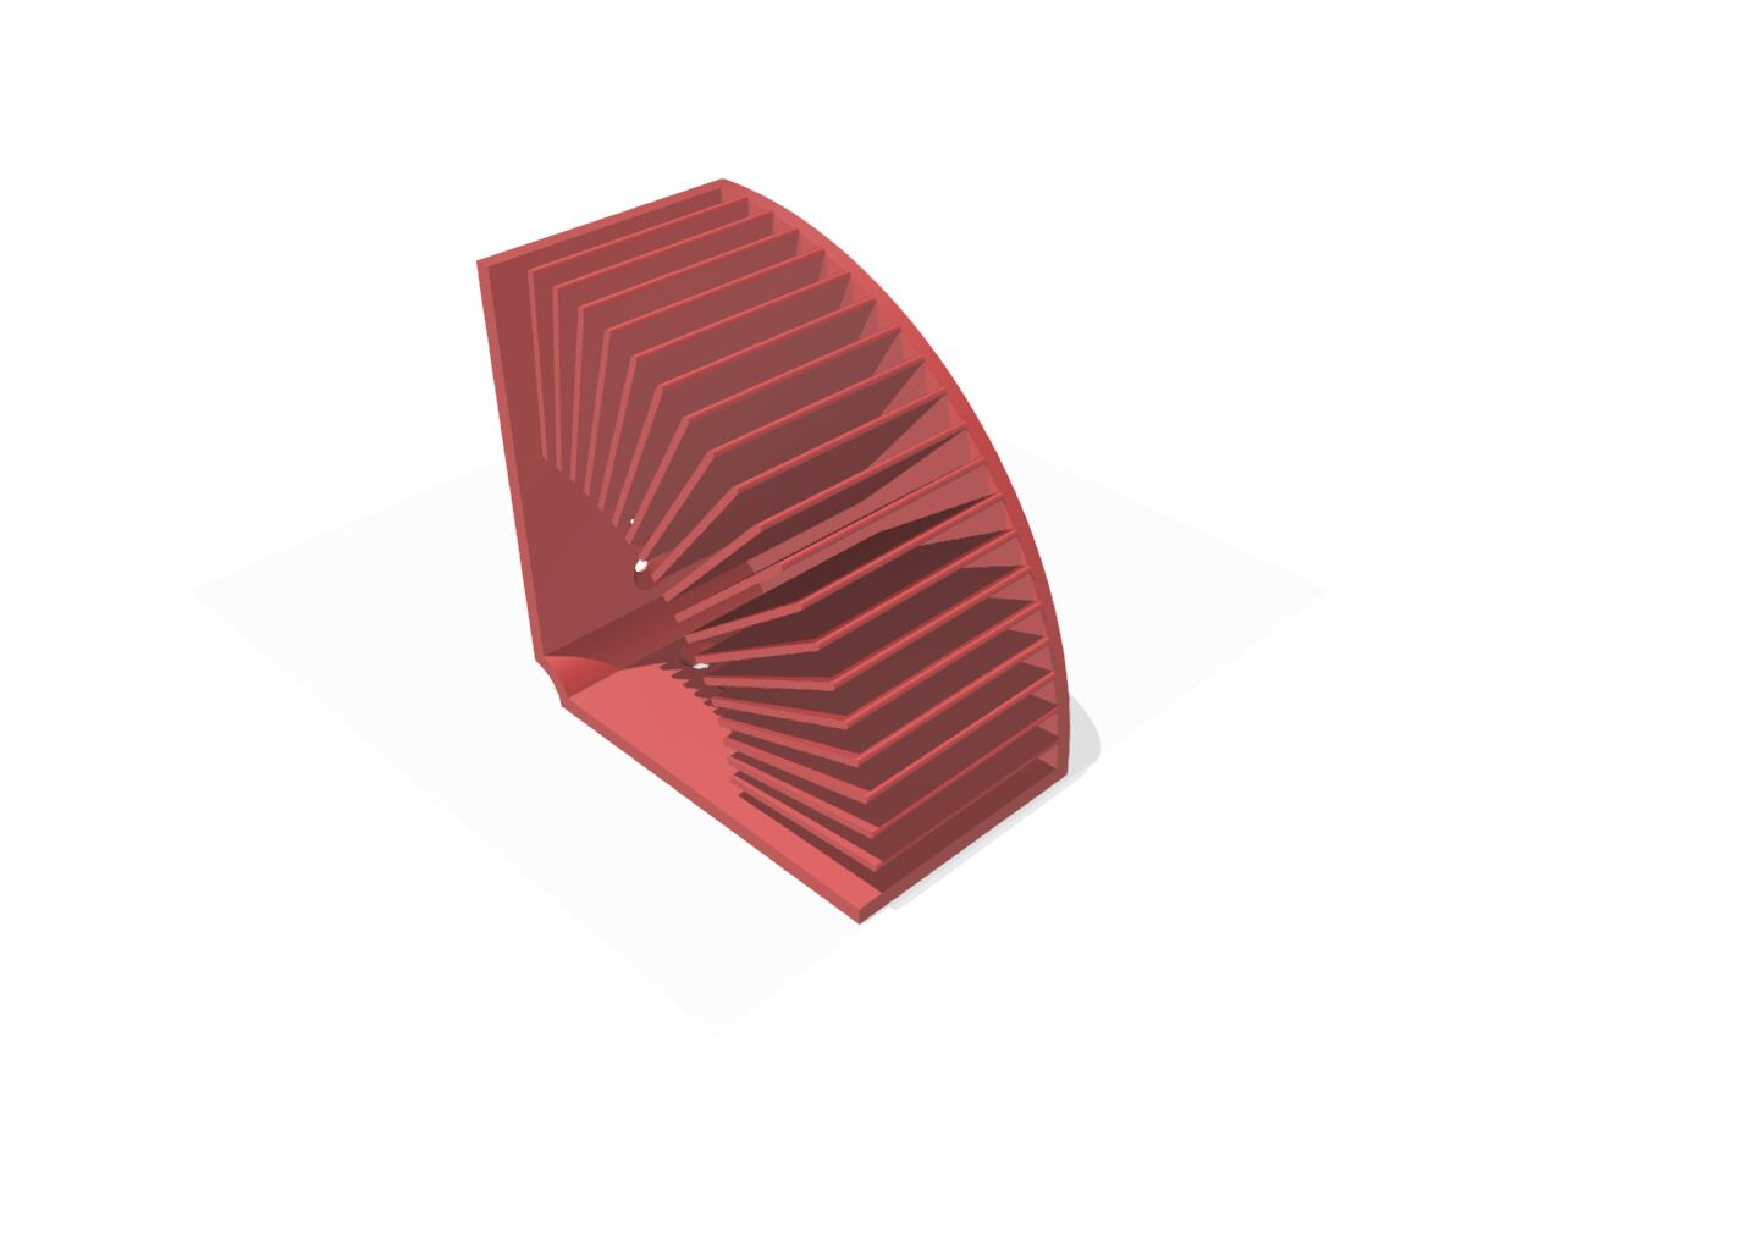
\includegraphics[scale=0.5,page=1]{fig/mech/LagerRad20F}
    \caption{Version 1: Lagerrad 20 Fächer (geöffnete Außenwand zur vereinfachten Ansicht)}
\end{figure}

In der oben angezeigten Grafik wurde die Außenwand entfernt, um eine bessere Einsicht in das Bauteil zu bekommen.
Durch die 20 Unterteilungen muss der Schrittmotor genauere Positionen anfahren, außerdem wäre der Aufwand beim Produzieren groß. Aus diesem Grund
entschieden wir uns die Unterteilungen zu minimieren und kamen zu dem Entschluss, dass 4 Unterteilungen für ein optimales Mischen ausreichen. Diese Konstruktion
wurde nach einem Stecksystem entworfen, sodass man die einzelnen Teile herstellen kann und diese danach zusammenstecken und verkleben kann.

\begin{figure}[H]
    \centering
    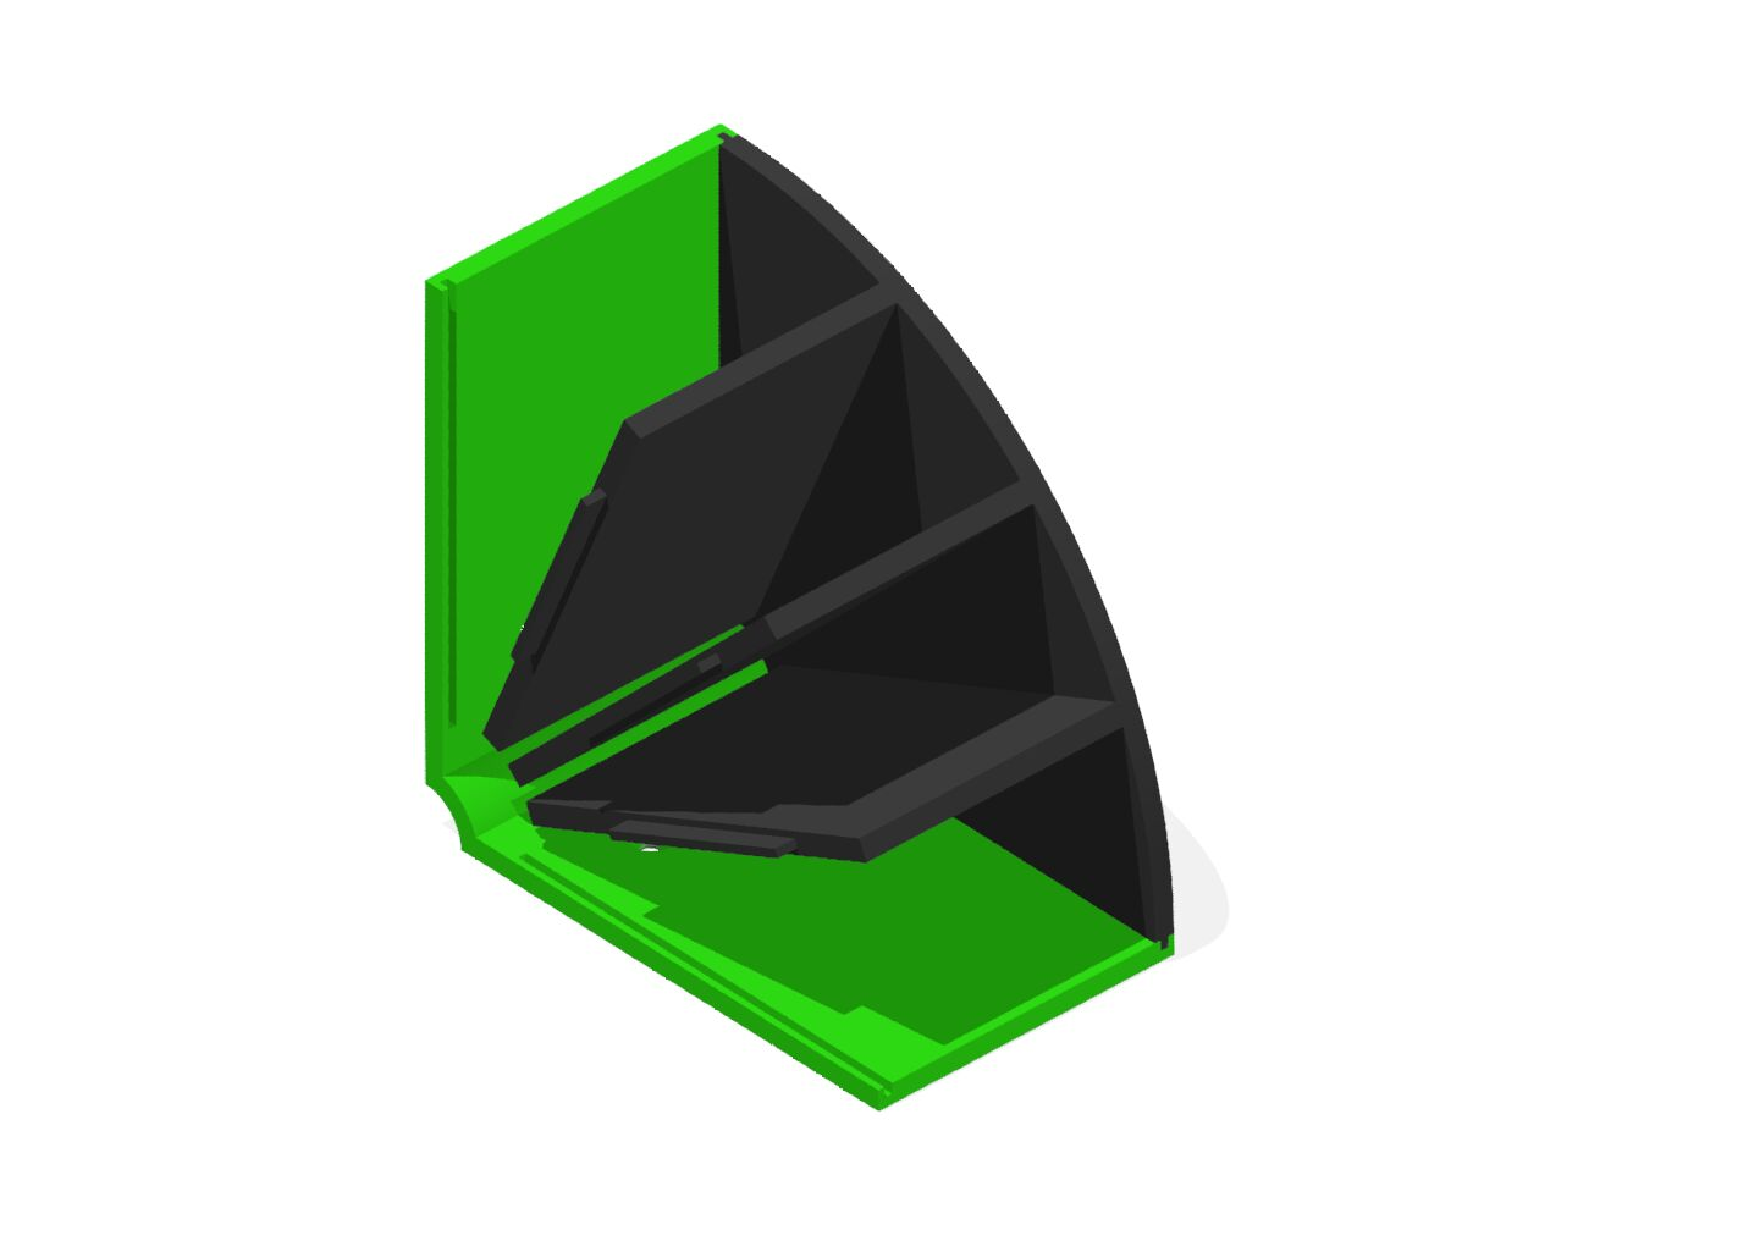
\includegraphics[scale=0.5,page=1]{fig/mech/LagerRad4F}
    \caption{Version 2: Lagerrad 4 Fächer (geöffnete Außenwand zur vereinfachten Ansicht)}
\end{figure}


Auch in der oben gezeigten Grafik wurde die Außenwand entfernt, um das Bauteil besser zu veranschaulichen.
Das Lagerrad besteht aus mehreren Einzelteilen:

\subsubsection{Außenwände}
Die Außenwände wurden in der Form eines Teiles eines Kreises konstruiert und geben somit die Form des Lagerrades vor. Sie besitzen jeweils 2 Laschen an der äußeren Seite, diese verbinden die Außenwände später mit den Seitenwänden des Lagerrades.
Außerdem besitzen sie jeweils 3 Ausfräsungen auf ihrer Grundfläche, über die sie später mit den Trennplatten versteckt werden. Bei der Konstruktion der Ausfräsungen ist dabei zu achten, dass sie etwas größer als benötigt gezeichnet werden, da bei der
Fertigungsart des 3D-Druckens Innenbohrungen und Innenfräsungen durch die Ungenauigkeit des Druckers kleiner gedruckt werden. Wie auch bei den Innenfräsungen müssen die Laschen auf der Außenseite etwas kleiner konstruiert werden, da diese wiederum beim
Drucken größer gedruckt werden, als sie ursprünglich gezeichnet wurden.

\subsubsection{Seitenwände}
Diese Bauteile verbinden das Lagerrad mit dem Lagerradhalterungsmodul. Sie besitzen auf der äußeren Seite der Grundfläche
jeweils 2 Auskerbungen. Über diese werden sie mit den Laschen der Außenwände verbunden. Um einen Durchgang für die Welle zu schaffen,
schließen die Bauteile auf der unteren Seite nicht im rechten Winkel ab, sondern sind nach innen radial abgerundet.
Je Bauteil sind 2 Bohrungen vorhanden, über diese wird es mit dem Lagerradhalterungsmodul verbunden.
Die Bohrungen sind als Senklochbohrungen ausgeführt, da somit die Schraube komplett in das Bauteil versenkt werden kann
 und das Hineinrutschen der Karten in das Lagerrad nicht behindert wird.

\subsubsection{Trennplatte}
Um die einzelnen Lagerfächer zu unterteilen, ist die Trennplatte konstruiert worden. Dieses Bauteil ist ein einfacher
Quader mit je 2 Laschen an den Außenseiten. Diese Laschen werden mit den Ausfräsungen der Außenplatte versteckt.
Hierbei ist wieder zu achten, dass die Laschen kleiner konstruiert werden, da sie durch den 3D-Druck an Größe zunehmen
werden.

\subsection{Konstruktion des Lagerradhalterungsmoduls}
Um das Moment der Welle effektiv von der Welle zum Rad zu übertragen, wurde ein Lagerradhalterungsmodul entworfen. Dieses Modul wird
benötigt, da das Wellenmoment nicht effektiv an einem 3D-gedruckten Bauteil angreifen kann, da das gedruckt PLA
die kontinuierlichen Richtungswechsel sowie das abrupte Bremsens des Motors in Kombination mit der
Trägheit des Lagerrades nicht standhalten würde. Dieses Modul besteht aus folgenden Einzelteilen:

\subsubsection{L-Grundplatte}
Dieses Bauteil, siehe Abbildung ......., verbindet die Motorwelle sowie die Lagerwelle mit der Verbindungsplatte und somit auch das Lagerrad.
Es überträgt somit auch das Moment des Motors. Es besitzt je 4 Bohrungen mit Zylinderschraubensenkungen, über die sie mit
der Verbindungsplatte verbunden wird. Außerdem besitzt sie eine Bohrung mit einer Querbohrung. Über diese werden die
Wellen geführt und mit einer Schraube am Bauteil fixiert.
Dieses Bauteil wurde ursprünglich aus Aluminium gefertigt, durch Versuche mit einer 3D-gedruckten L-Grundplatte zeigte
sich jedoch, dass diese sich genauso gut eignet und optisch ansprechender ist. Um nicht in Konflikt mit dem Lagerrad
zu stehen, hat das Bauteil jeweils 2 Ausbuchtungen nahe der Welle.

\subsubsection{Verbindungsplatte}
Die Verbindungsplatte nimmt das von der L-Grundplatte aufgenommene Moment des Motors und überträgt es an das Lagerrad weiter.
Sie wurde als einfacher Aluminiumquader konstruiert und besitzt insgesamt 6 Bohrungen. Zwei Bohrungen sind auf der
Grundfläche des Bauteils und besitzen ein Gewinde. Diese verbinden das Lagerradhalterungsmodul mit dem Lagerrad. Je 2
Bohrungen sitzen auf der Unterseite sowie auf der Oberseite der Verbindungsplatte und sind ebenfalls mit Gewinde
ausgeführt, durch diese Gewindebohrungen wird das L-Bauteil mit der Verbindungsplatte verbunden.
Dieses Bauteil wurde aus Aluminium gefertigt, da es problematisch ist ein Gewinde in PLA zu schneiden, außerdem spielt
das zusätzliche Gewicht des Aluminiums bei diesem Modul nur eine geringe Rolle.

\subsubsection{Motorwelle}
Um das Moment vom Motor auf die L-Grundplatte zu übertragen, wird die Motorwelle benötigt. Diese ist eine einfache Welle
mit einer Gewindebohrung am äußeren Ende der Welle. Diese dient dazu, die Welle mit der L-Grundplatte zu verbinden.
Am anderen Ende ist die Welle über die Kupplung mit dem Motor verbunden.
Die Welle wurde an der Drehbank gefertigt und anschließend an der Fräsmaschine die Gewindebohrung gebohrt.

\subsubsection{Lagerwelle}
Die Lagerwelle unterscheidet sich von der Motorwelle lediglich durch ihre Länge. Sie wird auf der einen Seite mit der
L-Grundplatte verschraubt, auf der anderen Seite wird sie mit dem Zweiloch-Flanschlager auf der Vorderseite des Gehäuses über
2 Wurmschrauben geklemmt.

\begin{figure}[H]
    \centering
    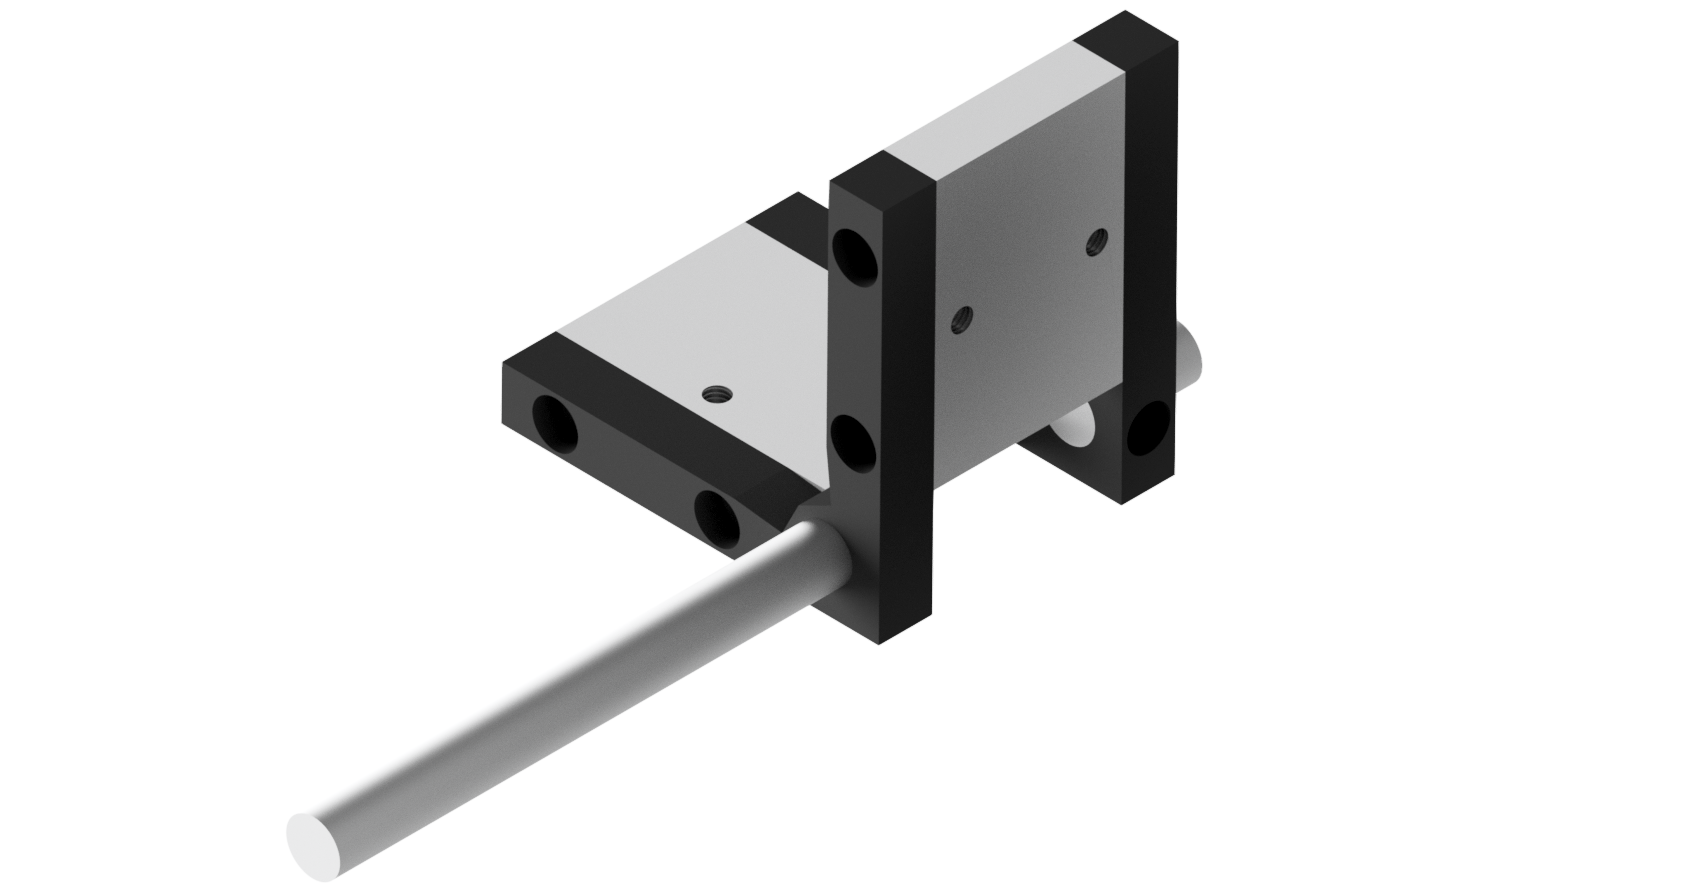
\includegraphics[scale=0.25,page=1]{fig/mech/LagerRadGruppekomplett}
    \caption{Lagerradhalterungsmodul}
\end{figure}

\subsection{Konstruktion der Motorhalterungsgruppe}

Die Motorhalterung, siehe Abbildung ......, hat den Zweck den Motor an das Gehäuse zu befestigen und ihn somit für die Welle auszurichten. Der ausgewählte Schrittmotor
besitzt eine mitgelieferte Montagehalterung die mit 4 Schrauben an den Motor geschraubt wird. Die Motorhalterung entspricht dem Nema 17
Standard und ist somit universal für Motoren dieser Norm anwendbar. Die Motorhalterung wird mittels 2 Schrauben an einen verzinkten Edelstahlwinkel angeschraubt, ist aber
in der Position noch Einrichtbar. Der Winkel wird über 4 Schrauben mit dem Gehäuse aus Polycarbonat verschraubt.

\subsection{Konstruktion des Kartenhalterungsmodul}
Die Karten müssen nach dem Einführen in die Maschine und nach dem Auswerfen aus dem Lagerrad zwischengelagert werden, da sie
von dem Hubmagneten und dem Saugnapf einzeln aufgehoben und ausgegeben werden. Für diese Aufgabe kommt das Modul der
Kartenhalterung, siehe Abbildung ...., zum Einsatz. Dieses Modul muss sicherstellen, dass genug Platz für mindestens 20 gewöhnliche Spielkarten  mit den Maßen 100 x 66
vorhanden ist. Das Modul besteht aus mehreren einzelnen Bauteilen:

\subsubsection{Sensorhalterung}
Die Sensorhalterung, siehe Abbildung ...., dient dazu den kapazitiven Sensor zu befestigen. Dieser wird mithilfe zwei Muttern und zwei Sicherungsringen
über das Gewinde des Sensors befestigt. Durch diese spezielle Befestigungsart kann man den Sensor in der Höhe einrichten und ihn so
auf andere Bauteile abstimmen. Die Sensorhalterung wird über 4 Bohrungen mit dem Kartenlager verschraubt.

\subsubsection{Kartenlager}

Um 20 Karten zwischenzulagern wird ein Kartenlager, dass in Abbildung .... zu sehen ist, benötigt. Dieses Lager hat eine Ausnehmung auf der oberen Seite in der die Karten
eingeführt werden, auf der unteren Seite besitzt es eine Öffnung, die Platz für eine Karte zum Herausfallen bietet. Diese Öffnung ist auf
einer Höhe von 11 mm, sodass die eingelagerten Karten nicht selbständig  herausfallen, sondern erst durch das Heben des Hubmagnetes.
Das Kartenlager besitzt außerdem zwei Einkerbungen in einer Höhe von 11 mm auf den Seiten, diese bieten Platz für einen Gummiabstreifer,
dessen Funktion ist es mehrerer auf einmal aufgehobene Karten zu trennen und somit sicherzustellen das nur eine Karte ausgegeben wird.
Der Gummiabstreifer stellt auch sicher, dass die Karte aus der Kartenhalterung herausgeworfen wird und nicht wieder zurück auf den Kartenstapel
fällt. \\
Das Lager besitzt außerdem eine Ausnehmung auf der Unterseite, durch diese Ausnehmung wird der Sensor geführt und so eingestellt,
dass er plan mit der Grundfläche des Lagers ist. Die Ausnehmung ist auch so konstruiert, dass sie groß genug ist um vom Sensor
nicht erkennt zu werden, wenn dieser auf seiner maximalen Sensibilität konfiguriert ist.\\
Verbunden ist das Kartenlager über 4 Schrauben mit dem Abstreifer und der Sensorhalterung.

\subsubsection{Abstreifer}

Der Abstreifer, siehe Abbildung ...., dient dazu, Karten die nicht durch das Lösen des Unterdrucks vom Saugnapf fallen und noch an ihn Haften
abzuwerfen. Er ist so konstruiert, dass er beim Einfahren des Hubmagnetes die Karten leicht berührt und diese somit vom
Saugnapf löst. Er besitzt eine Öffnung auf seiner Grundfläche, die groß genug für unseren ausgewählten Saugnapf ist.\\
Seitlich besitzt es zwei Erhebungen mit jeweils zwei Durchbohrungen, über diese wird das gesamte Modul über jeweils 2 Aufhänger
mit dem Gehäuse verschraubt. \\
Der Abstreifer wird durch 4 Schrauben mit dem Kartenlager und mit der Hubmagnetaufhängung  verbunden.

\subsubsection{Hubmagnetaufhängung}

Die Hubmagnetaufhängung, siehe Abbildung ...., besteht aus 2 symmetrischen Bauteilen. Diese Bauteile, die die Form eines Trapezes besitzen, fixieren den
Hubmagneten mit jeweils 4 Schrauben pro Seite auf seiner Position. Das Bauteil ist so konstruiert, dass der Hubmagnet, wenn er
vollkommen Ausgefahren ist, mit dem montierten Saugnapf die Grundfläche des Kartenlagers erreicht, und somit in der Lage ist,
alle Karten anzusaugen.\\
Die Aufhängung ist mit jeweils 2 Bohrungen mit dem Abstreifer verschraubt und somit an dem gesamten Modul befestigt.

\subsubsection{Aufhänger}
Um das Modul in die gewünschte Position zu bringen werden Aufhänger, die in Abbildung .... zu sehen sind, benötigt, diese sind mit dem Polycarbonatsgehäuse verschraubt.
Da die Aufhänger keine Krafteinwirkungen ausgesetzt sind, können diese dünn und Materialsparend konstruiert werden.
Da das Kartenhalterungsmodul zweimal an verschiedenen Position zum Einsatz kommt, wurden zwei unterschiedliche
Aufhänger konstruiert.\\\\
\textbf{Aufhänger Oben:} \\
Dieser Aufhänger, siehe Abbildung ...., wird über jeweils zwei Schrauben an der TopPlatte des Gehäuses befestigt und hält das obere Kartenhalterungsmodul in Position.
Das Modul wird über zwei versetzte Bohrungen mit dem Aufhänger verschraubt, diese sind so konstruiert, dass das Modul in einem
Winkel von 60° befestigt wird.
Durch die niedrige Höhe des Aufhängers ist auch durch die dünne Bauweise genug Stabilität gegeben.\\\\
\textbf{Aufhänger Unten:}\\
Das zweite Modul, welches in Abbildung ... zu sehen ist, befindet sich nach dem Lagerrad und wird vom unteren Aufhänger in Position gehalten. Der untere Aufhänger
wird mit 2 Schrauben mit der Grundplatte des Gehäuses verschraubt. Durch die dünne Bauweise des Aufhängers und die
große Höhe führt dies zu einer Instabilität des Moduls und des Aufhängers in Querrichtung, dieses Problem ist jedoch irrelevant, da es
zu keiner Krafteinwirkung auf das Modul auf dieser Achse kommt. Um das Problem dennoch zu beheben, kann die Breite des
Aufhängers variiert werden oder eine Querstrebe bei der Konstruktion hinzugefügt werden, da somit der Materialaufwand beim 3D-Drucken gering bleibt.\\
Der Aufhänger wird wie der andere Aufhänger über jeweils 2 Schrauben mit dem Kartenhalterungsmodul verschraubt.

\subsubsection{Kartenführung}
Um das Einführen der Karten zu erleichtern und ohne Probleme zu ermöglichen besitzten die Module Kartenführungen.

\textbf{Kartenführung Modul 1 oben}
Das erste Modul besitzt eine Kartenführung, siehe Abbildung ..., diese fungiert wie ein Trichter, der die Karten in die richtige Position bringt.
Die Kartenführung wird nicht mit dem Kartenhalterungsmodul verschraubt, sondern
verklebt. Bei dieser Verbindung kann ohne Probleme eine Klebverbindung angewendet werden, da keine großen Kräfte auftreten, außerdem
ist sie platzsparender und einfacher zu realisieren. Die Berechnungen zu den Klebestellen finden sie unter ............ TODO

\textbf{Kartenführung Modul 2 oben}
Diese Kartenführung, siehe Abbildung ..., sorgt dafür, das die Karten, die aus dem Lagerrad geworfen werden nicht zu früh herausfallen,
sondern erst genau über der Öffnung des Kartenhalterungsmodul. Sie sind so entworfen, dass die Krümmung der Führungsfläche einen leicht
größeren Radius besitzt wie der Maximalradius des Lagerrades. Diese zwei Kartenführungen sind mittels Klebeverbindungen
an das Kartenhalterungsmodul befestigt, da keine großen Kräfte diese Bauteile angreifen.

\textbf{Kartenführung Modul 2 unten}
Die untere Kartenführung, die in Abbildung ... zu sehen ist, sorgt dafür, das Karten, die nicht rechtzeitig aus dem Lagerrad fallen und somit erst später
herausfallen nicht auf dem Boden der Maschine gelangen, sondern durch die Kartenführung weiter im Lagerrad bleiben. Diese Führung
wird durch ihre Größe und Postion nicht an dem Modul befestigt, sondern wird über jeweils 2 Schrauben mit dem Gehäuse
verbunden. Durch die lange Bauform und die geringe Stärke des Bauteils, sollten Querstreben in die Konstruktion eingeplant werden,
da die Kartenführungen sich sonst bei leichtem Berührungskontakt schon stark bewegen.

\subsection{Konstruktion der Kartenentnahme}
Die Kartenentnahme, die in Abbildung ... zu erkennen ist, befindet sich am unteren Ende der Maschine, sie dient dazu die Karten zwischenzulagern bis der Spieler
sie entnimmt. Sie besteht aus folgenden Einzelbauteilen:

\subsubsection{Entnahmeplatte }
Dies ist das Grundbauteil, siehe Abbildung ..., dieses Moduls, es fängt die Karten die vom Kartenhalterungsmodul ausgeworfen werden und lagert diese zwischen bis
der Spieler diese manuell entnimmt. Das Bauteil liegt in einem 45° Winkel und besitzt einen halbkreisförmigen Ausschnitt
an der Unterseite, der dazu dient, das Entnehmen der Karten zu vereinfachen. Der rechteckige Ausschnitt in der Mitte des
Bauteils dient als Ausschnitt für den Sensor, sodass dieser überprüfen kann, ob sich Karten in dem Bauteil befinden.

\subsubsection{Sensorhalterung}
Da bei der Kartenentnahme auch geprüft wird, ob noch Karten in der Entnahmeplatte liegen, wird eine Halterung für den
Sensor benötigt. Dieses Bauteil, siehe Abbildung ..., besitzt eine Bohrung, in der der Sensor durchgeführt wird und danach über zwei Muttern und
zwei Sicherungsringen befestigt wird. Die rechteckige Ausfräsung auf der unteren Seite der Sensorhalterung dient lediglich
für optische Zwecke und zur Materialverbrauchsminderung.

\subsubsection{Befestigungswinkel}
Da die Entnahmeplatte  in einen 45° zum Gehäuse montiert werden muss, wurden dafür einfache Winkel, die in Abbildung .... zu sehen sind, konstruiert und gefertigt.
Diese werden auf der einen Seite mit der Unterseite des Gehäuses verklebt, auf der anderen Seite mit der Entnahmeplatte.
Auch hier können wieder Klebeverbindungen genutzt werden, da keine großen Kräfte auf die Bauteile angreifen.

\subsubsection{Sensorhalterungswinkel}
Die beiden Sensorhalterungswinkel ermöglichen das fixieren der Sensorhalterung in einem Winkel von 45°, parallel zur
Entnahmeplatte. Sie werden jeweils mit der Unterseite des Gehäuses und mit der Sensorhalterung verklebt.

\subsection{Konstruktion der Endschalterhalterung}
Dieses Bauteil, dass in Abbildung ... zu sehen ist, hat die Funktion den Endschalter, der als Referenzpunkt für den Motor und das darauf montierte
Lagerrad gilt, zu befestigen. Es besitzt zwei diagonale Bohrungen, über die der Endschalter verschraubt wird.
Die Endschalterhalterung wird auf der Rückseite über zwei Bohrungen mit dem Polycarbonatgehäuse verschraubt.
Das Bauteil muss so stabil gebaut sein, dass es einen leichten Zusammenstoß mit dem Lagerrad aushält, falls dieses
den Referenzpunkt anfahren möchte.

\subsection{Konstruktion des Gehäuses}
Das Gehäuse soll bei dieser Maschine optisch ansprechen und so klein wie möglich gehalten werden. Für die Auswahl
des Gehäusematerials kamen diverse Materialien infrage:

\begin{table}[H]
    \centering
    \scalebox{0.8}{
    \begin{tabular}{|c|c|c|}
        \hline
        & \textbf{Vorteile}                                                                                                                                  & \textbf{Nachteile}                                                                                    \\ \hline
        \textbf{POLYCARBONAT (PC)}                    & \begin{tabular}[c]{@{}c@{}}sehr hohe Schlagfestigkeit\\ Transparent\\ leicht zu bearbeiten\\ geringes Gewicht\\ gute UV-Beständigkeit\end{tabular} & vergleichsweise teurer                                                                                \\ \hline
        \textbf{ACRYLNITRIL-BUTADIEN-STYROL (ABS)}    & \begin{tabular}[c]{@{}c@{}}geringes Gewicht\\ günstiger als PC\end{tabular}                                                                        & \begin{tabular}[c]{@{}c@{}}nicht für die Verwendung im Freien\\ nicht transparent\end{tabular}        \\ \hline
        \textbf{GLASFASERVERSTÄRKTES POLYESTER (GRP)} & \begin{tabular}[c]{@{}c@{}}Wetterbeständig\\ Stabil\\ Schlagfestig\end{tabular}                                                                    & \begin{tabular}[c]{@{}c@{}}teurer als PC\\ schwer zu bearbeiten\\ beträchtliches Gewicht\end{tabular} \\ \hline
    \end{tabular}}
    \caption{Vergleich der Gehäusematerialien}
\end{table}

Da wir unser Material bearbeiten müssen, es portabel gestalten wollen und kein großes Budget haben können wir
GRP als Gehäusematerial ausschließen. Unser Gehäuse sollte auch optisch ansprechend sein und den Innenaufbau unserer
Maschine zeigen, somit ist ABS auch ausgeschlossen, da es nicht transparent ist. Somit entschieden wir uns für
Polycarbonat als finales Gehäusematerial.

\subsubsection{Grundplatte}
Die Grundplatte ist die einzige Platte des Gehäuses, die nicht aus Polycarbonat besteht, sondern aus einem 12 mm dicken
Acrylglas, da uns dieses kostenlos zur Verfügung stand.\\
Um den unteren Aufhänger des Kartenhalterungsmoduls und die Kartenführung Modul 2 unten zu befestigen befinden sich 8
Bohrungen in der Mitte der Grundplatte. Diese Bohrungen sind mit einer Boden-seitigen Senkung versehen, somit kann die
Senkkopfschraube ganz in die Grundplatte gesenkt werden und behindert nicht die Stabilität der Maschine.
Des Weiteren befindet sich in jeder Ecke eine weitere Bohrung mit Boden-seitiger Senkung. Über diese Bohrung werden die
Winkel verschraubt, die die Grundplatte mit den restlichen Platten des Gehäuses verbindet.

\subsubsection{Seitenplatte Motor}
Diese Gehäuseplatte besitzt, genauso wie die Grundplatte, 4 Bohrungen an den Ecken der Platte um sie über Winkel
mit den anderen Platten zu verbinden. Weiters hat sie 4 Bohrungen im mittleren Bereich, über diese Bohrungen wird
der Winkel der Motorhalterungsgruppe verschraubt. Darüber hinaus besitzt sie eine innenseitige Einfräsung in der sich
zwei weitere Bohrungen befinden. Diese Bohrungen werden für den Netzteilstecker sowie für den Taster benötigt.
Die Einfräsung ist notwendig, da diese beiden Bauteile ein Gewinde besitzen, über die sie mit dem Gehäuse verbunden werden,
jedoch ist das Gewinde zu kurz für die dicke des Polycarbonats.

\subsubsection{Seitenplatte Lager}
Da diese Platte die Vorderseite des Gehäuses ist, ist auf ihr auch das Liquid-Crystal-Display montiert. Um diesen zu montieren
hat die Platte eine rechteckige Ausfräsung im oberen Mittelbereich. Seitlich ober und unter der Ausfräsung befinden sich
je Seite 2 Langlöcher, über diese wird das Display mit dem Gehäuse verschraubt.
Unter dem Display besitzt diese Platte zusätzlich 2 Senklochbohrungen, über diese wird das Flanschlager verschraubt.
Zuletzt besitzt diese Platte auch 4 Bohrungen an den Ecken, über die sie mit den anderen Platten verschraubt wird.

\subsubsection{Frontplatte}
Wie die vorherigen Platten wird auch diese Platte über 4 Bohrungen mit den Winkeln verschraubt.
Ansonsten hat diese Platte des Gehäuses nur 2 weitere Bohrungen, über die die Endschalterhalterung verschraubt wird.

\subsubsection{Ausgabenplatte}
Da über diese Platte die Karten entnommen werden, besitzt die Ausgabenplatte eine rechteckige Einfräsung auf der unteren
Seite.
Weiters besitzt sie wie die anderen Platten 4 Bohrungen an den Ecken.

\subsubsection{Topplatte}
Die Topplatte oder auch der "Deckel" des Gehäuses hat eine rechteckige Einfräsung in der die Kartenführung Modul 1 oben
gesteckt wird. Nach der Einfräsung besitzt diese Platte noch 4 Bohrungen, über die der Aufhänger des Kartenhalterungsmodul
befestigt wird.
Wie auch bei allen anderen Platten besitzt diese Platte auch 4 Bohrungen an ihren Eckpunkten.

\section{Berechnungen und Dimensionierungen}
\subsection{Auswahl des Motors}
TODO\\
\textbf{Eckdaten des gewählten Motors}
\begin{itemize}
    \item Motortyp: Bipolarer Schrittmotor
    \item Schrittwinkel: 1,8 Grad
    \item Haltemoment: 0,59 Nm
    \item Bemessungsstrom / Phase: 2,0 A
    \item Gewicht: 380 g
    \item Rahmengröße 41 mm x 41 mm
\end{itemize}
\subsection{Auswahl der Vakuumaktorik}
\subsubsection{Auswahl der Vakuumpumpe\footfullcite{Sauggreifer}}
Um die Vakuumpumpe auszuwählen, muss zuerst die erforderliche Druckdifferenz berechnet werden.
Da die Karten liegend angehoben werden kommt für die Berechnung der theoretischen Haltekraft der typische Lastfall 1
zum Einsatz. Zwar wird dieser für eine vertikale Kraftrichtung eingesetzt, und nicht wie bei dem Beispiel in einem
60° Winkel, dennoch ist er der Lastfall der den am nächsten kommt.
Die theoretische Haltekraft wird mit folgender Formel berechnet:
\begin{equation}
    F_{TH} = m \cdot (g + a) \cdot S
\end{equation}

    F\textsubscript{TH}.... theoretische Haltekraft [N] \\
    m.... Masse [kg]\\
    g.... Erdbeschleunigung [9,81 m/s²]\\
   a.... Beschleunigung der Anlage [m/s²]\\
    S.... Sicherheitsfaktor \\

Die Masse einer standardmäßigen  Spielkarte liegt bei 2 Gramm, darum wird mit einem Wert von m = 2 g gerechnet.
Die maximale Wegbeschleunigung des Saugnapfes wird beim Einziehen des Hubmagnetes erreicht und
beträgt 1,8 m/s²,
daher wird für die Beschleunigung a = 1,8 m/s² eingesetzt. Da ein geringer Unterdruck zur nächsten Karte herrscht, wird eine Sicherheit von 20 gewählt.
Setzt man die Werte in die Formel ein, bekommt man folgendes Ergebnis: \\
\[F_{TH}=0,002kg\cdot (9,81\frac{m}{s^{2}}+1,8\frac{m}{s^{2}})\cdot 20\]
\[F_{TH}= 0,4644N\]

Um die Druckdifferenz zu berechnen muss als Erstes die Fläche des Saugers berechnet werden.
Mit einem Durchmesser des Saugers von 20 mm ergibt sich eine Fläche von:
\[A=r^{2}\cdot \pi\]
\[A=0,02^{2}\cdot \pi\]
\[A=0,001257m^{2}\]

Setzt man die Werte in die Formel ein, bekommt man folgende Druckdifferenz:
\[\triangle P=\frac{F_{TH}}{A}\]
\[\triangle P=\frac{0,4644N}{0,001257m^{2}}\]
\[\triangle P=369,4511Pa\]

Da der berechnete Wert unbeachtlich klein ist, kann eine möglichst kleine Pumpe ausgewählt werden. Diese beansprucht
wenig Platz, braucht wenig Strom und ist leise. Schlussendlich wurde eine Pumpe mit einer Leistung von 2,15W und einer
Spannung von 5V DC ausgewählt.\\
\textbf{Daten der Pumpe}
\begin{itemize}
    \item Spannung 5V (max 6V)
    \item Druck: > 400 mmHg (> 53329 Pa)
    \item Verbrauch: 430 mA
    \item Lautstärke: 63 dB
    \item Durchflussrate: > 1,8 Liter pro Minute
\end{itemize}



\subsubsection{Auswahl der Valve}
Da der Saugnapf nicht immer einen Unterdruck haben darf, wird eine Valve benötigt, dieses Bauteil fungiert wie ein
Schalter, der dafür sorgt ob, der Saugnapf einen Unterdruck bekommt oder nicht. Die einzige Voraussetzung  der Valve war es, nicht zu viel Spannung zu verbrauchen, daher entschieden
wir uns für eine Valve mit 5 V Spannung.
\textbf{Eckdaten der ausgewählten Valve}
\begin{itemize}
    \item Nennspannung: DC 6V
    \item geeigneter Spannungsbereich:DC 5V - DC 6V
    \item Strom: 220 mA
    \item Leistung: <2W
    \item Druckbereich: 0-350 mmHg
\end{itemize}




\section{Fertigung der Bauteile}
\subsection{Werkstoffwahl}
Anfangs stellte sich die Frage mit welchem Werkstoff die Prototypen sowie die Fertigen Bauteile der
Maschine produziert werden sollen. Da die Bauteile ein niedriges Gewicht haben sollen, billig und schnell produzierbar
sein sollten wurde Kunststoff ausgewählt. Es wurden folgende Arten zur Verarbeitung von Kunststoff in Betracht gezogen:
\subsubsection{Extrudieren\footfullcite{Kunststoffverarbeitung Extrudieren}}
Das geschmolzene Material wird beim Extrudieren über Düsen gepresst. Über Ringförmige Düsen können Rohre entstehen,
über Schlitzförmige können Platten entstehen, somit entspricht der Querschnitt der Düse immer auch den Querschnitt
des erzeugten Profils. Der Vorteil dabei ist, dass sogar Formen mit Hohlräumen an einem Tag herstellbar sind.
Die erzeugten Platten werden oftmals noch weiterverarbeitet, indem man sie erwärmt und über eine Form zieht, oder durch
Vakuum und Druck in die gewünschte Form bringt.
Es gibt noch diverse andere Arten von Extrudern, wie den Schneckenextruder, dieser lässt sich weiter unterteilen in den
Einschnecken-, gegenlauf Doppelschnecken- und gleichläufige Doppelschneckenextruder. Der Vorteil der Doppelschneckenextruder
liegt dabei in ihrem guten Mischungsverhältnis, jedoch sind Einschneckenextruder um vieles günstiger.
Andere Bauformen des Extruders wären der Kolbenextruder sowie der Planetwalzenextruder.
Für Keramikmaterialien werden in der Regel Kolbenextruder eingesetz.
Um PVC-Folien Herzustellen werden am häufigsten Planetwalzenextruder benutzt.

\subsubsection{Spritzgießen\footfullcite{Kunststoffverarbeitung Spritzgießen}}
Über das Spritzgießen können komplexe Bauteile mit einer hohen Qualität hergestellt werden. Die Maschine besteht dabei aus
einer sogenannten Spritzeinheit und einer Schließeinheit. Die Spritzeinheit besteht aus einem Extruder mit einer
beweglichen Schnecke, diese stößt die Polymerschmelze durch die Vorwärtsbewegung der Schnecke in das Werkzeug aus.
Um das Werkzeug zu öffnen und zu schließen und somit den Ausstoß des Polymeres zu ermöglichen wird die Schließeinheit
benötigt.
Bei Beginn des Spritzgusses wird eine rotierende Schnecke mit einem Granulat oder einem Pulver befüllt. Das Material
wird danach durch die rotierende Bewegung der Schnecke geschmolzen und nach vorne befördert. Das geschmolzene Material
staut sich an der Spitze, da das Werkzeug durch die Schließeinheit noch nicht geöffnet wurde und somit entsteht ein
hoher Druck. Da die Schnecke beweglich gelagert ist, dreht sich diese selbst aus dem verdichteten Polymere heraus.
Wird das Material dann eingespritzt, öffnet sich das Werkzeug und die Schnecke wird unter Druck gesetzt, sodass das
Material in die gewünschte Form gespritzt  werden kann.
Beim Spritzgießen wird immer mehr Material mitgedruckt, da sich beim Abkühlen des Spritzgusses das Volumen leicht
verringert.
Da das Werkzeug des Spritzgusses sehr teuer ist, müssten einige tausend Stück unserer Bauteile hergestellt werden,
sodass sich der Spritzguss rentiert.

\subsubsection{Blasformen\footfullcite{Kunststoffverarbeitung Blasformen}}
Bei dieser Form der Kunststoffverarbeitung wird Druckluft in ein Schlauchstück eingeblasen, das zuvor über ein Werkzeug
extrudiert wurde. Über dieses Verfahren können somit Hohlkörper wie Flaschen oder Kanister hergestellt werden.
Über ringförmige Düsen können auch Folien hergestellt werden, dieses Verfahren wird dann auch als Folienblasen bezeichnet.

\subsubsection{Kalandrieren\footfullcite{Kunststoffverarbeitung Kalandrieren}}
Beim Kalandrieren schmilzt man eine Kunststoffmasse zwischen zwei erwärmten, sich gegeneinander drehenden Walzen auf.
Weitere Walzen werden für die benötigte Dicke der Folie dazugeschaltet und sorgen gleichzeitig für die Homogenisierung.
Über das Kalandrieren werden Platten oder Folien hergestellt, man kann aber auch andere Materialien wie Metalle, Papier
oder Gummi verwenden.

\subsubsection{Rotationsformen\footfullcite{Kunststoffverarbeitung Rotationsformen}}
Bei diesem Produktionsverfahren werden größere, hohle und nahtlose Kunststoffteile hergestellt. Es befindet sich
ein geschmolzenes Kunststoffgranulat in einer rotierenden Form, dieses Granulat setzt sich beim Auskühlen an den
Rand der rotierenden Form ab und erzeugt somit eine hohle Kunststoffform.
Der Vorteil hierbei liegt bei den niedrigeren Kosten, jedoch ist man nur in der Lage primitivere Formen herzustellen,
die hohl sind.

\subsubsection{Verarbeitung von duroplastischer Kunstoffe\footfullcite{Kunststoffverarbeitung Duroplasten}}
Um duroplastische Kunststoffe zu verarbeiten, müssen sie mittels Synthese in die gewünschte Form gebracht werden, da sie
nicht wärmeformbar sind. Dazu werden meist pulverförmige Vorprodukte direkt in eine Form gebracht, und nach Bedarf
Farb- oder Zusatzstoffe beigefügt. Danach werden sie unter Katalysator- und Wärmeeinfluss zum Endprodukt ausgehärtet.
Durch dieses Verfahren können auch metallische Werkstoffe mit Duroplasten verbunden werden, wie zum Beispiel
Glas-verstärkte Kunststoffe (GFK) die vielfältig in der Luft- und Wasserfahrt zum Einsatz kommen.

\subsubsection{Kleben\footfullcite{Kunststoffverarbeitung Kleben}}
Kleben ist ein Fügeverfahren von Kunststoffen, bei dem meist Duroplasten und Elastomere zusammengefügt werden.
Jedoch benötigt man dazu Kunststoffe mit polaren Egenschaften, um eine erfolgreiche Klebeverbindung zu garantieren.
Um diese Eigenschaften zu erschaffen müssen viele Kunststoffe mit Korona- oder Plasmabehandlung vorbereitet werden,
um die notwendige Benetzbarkeit aufzuweisen.\\
Physikalische Kleber können in drei Kategorien eingeteilt werden:
\begin{itemize}
    \item \textbf{Verdunstung}: Diese Kleber härten durch Verdunstung des Lösemittels aus.
    \item \textbf{chemische Kleber}: Aushärtung durch chemische Reaktion
    \item \textbf{molekulare Struktur}: Besitzen bereits vor dem Auftragen über eine molekulare Struktur
\end{itemize}

\subsubsection{Schweißen\footfullcite{Kunststoffverarbeitung Schweißen}}
Schweißen ist das zweite Fügeverfahren für Kunststoffe, bei diesem Verfahren muss das Material in erster Linie die
Fähigkeit zum Schmelzen verfügen. Da nur Thermoplaste diese Eigenschaft besitzt, ist es der einzige Kunststoff, der sich gut
zum Schweißen eignet. Für das Erwärmen und Aufschmelzen des Materials können unterschiedliche Techniken angewendet werden:
\begin{itemize}
    \item elektrische Induktionsheizung (Heizelementschweißen)
    \item heiße Druckluft (Warmgasschweißen)
    \item Licht- oder Laserstrahlung (Strahlungsschweißen)
    \item Reibung (Reibungsschweißen)
\end{itemize}

\subsubsection{3D-Druck}
Der 3D-Druck ist zwar kein Umformverfahren oder Fügeverfahren, sondern ein Urformverfahren mit dem man schnell und mit hoher Genauigkeit Kunststoffteile
drucken kann. Da das 3D-Drucken billig, schnell und eine hohe Genauigkeit hat, nahmen wir es zum Bau unserer Prototypen. Genaueres zum 3D-Druck finden
Sie unter Kapitel 1.7.2 3D-Druck.

\subsection{3D-Druck}
Das Verfahren des 3D-Drucks wurde aufgrund seiner preisgünstigen Fertigung, seiner Schnelligkeit und der Tatsache
ausgewählt, dass uns der 3D-Drucker der HTBLA Kaindorf zur Verfügung stand.
\subsubsection{Grundlagen\footfullcite{3D-Druck Grundlagen}}
Der 3D-Druck fungiert im Prinzip der additiven Fertigung, das heißt, er fertigt Objekte aus 3D-Modelldaten Schicht für Schicht
durch das Verbinden von Materialien. Es unterscheidet sich von dem traditionellen subtraktiven Verfahren dadurch,
das bei ihnen eine abtragende Kraftwirkung herrscht, wie zum Beispiel Fräßen oder Bohren. Formende Verfahren
erreichen die gewünschte Form durch Einfluss von mechanischen oder thermischen Kräften, wie zum Beispiel das Biegen oder
Pressen. Beim additiven  Verfahren jedoch wird die gewünschte Form durch Erzeugen von Geometrie erreicht, so werden Schichten
hinzugefügt oder aufgetragen. Als hybrides Verfahren bezeichnet man jene, die sich nicht in eine dieser Kategorien
Unterbringen lassen oder jene die mehrere dieser Verfahren miteinander verbinden.

\textbf{Produktionsverfahren}
Produktionsverfahren lassen sich in 4 Kategorien einteilen:
\begin{itemize}
    \item \textbf{manuelle Verfahren}: Dieses Verfahren beschreibt vereinfacht gesagt die klassische  Handarbeit, wie zum Beispiel das Biegen eines Drahtes (formend), das Hobeln von Holz (subtraktiv) oder das Auftragen von einem Guss (Additiv).
    \item \textbf{mechanische Verfahren}: Das mechanische Verfahren entwickelte sich aus dem manuellen, die Kraftwirkung wird dadurch von Hebeln, Seilzügen oder anderen Systemen erzeugt.
    \item \textbf{elektrische Verfahren}: Beim elektrischen Verfahren wird die Kraftwirkung mithilfe von elektrischem Strom erzeugt. Ein Beispiel dafür wäre der Schmelzuguss, da die Schmelztemperatur dabei von einem elektrisch angetriebenen Heizsystem generiert wird.
    \item \textbf{digitale Verfahren}: Das digitale Verfahren ist eine Erweiterung des elektrischen Verfahrens, wird aber zusätzlich noch mit einem Computersystem angesteuert. Ein Biegeroboter wäre ein Beispiel für ein digital formendes Verfahren, ein 3D-Drucker wäre dadurch ein digital additives Verfahren.
\end{itemize}

\subsubsection{Arten des 3D-Drucks}
\textbf{3D-Druck mit Pulver\footfullcite{3D-Druck Pulverdruck}}
Dieses Verfahren ist ein fortgeschrittenes Verfahren aus dem "Additive Layer Manufacturing" Bereich, Pulver wird dabei
als Grundlage für den 3D-Druck verwendet. Ein solcher Drucker besitzt mehrerer Druckköpfe, diese fungieren ähnlich wie
die eines normalen Druckers, jedoch wird statt Tinte flüssiges Bindemittel extrudiert. Zur Vorlage des Drucks wird daher das
3D-Modell in vielen 2D-Layers aufgeteilt, diese 2D-Layers dienen auch als Datengrundlage.
Als Erstes wird beim Verfahren das unterste Layer über den Druckkopf mit einem flüssigen Bindemittel auf die Pulverschicht
aufgetragen. Danach wird eine dünne Schicht Pulver über das erste Layer gezogen. Anschließend fährt
das Pulverbett nach jedem Layer um die Höhe einer Pulverschicht nach unten und der Vorgang wiederholt sich mit dem
zweiten Layer. Dies geschieht so lange, bis das Bauteil fertig gedruckt worden ist.\\

\textbf{3D-Druck mittels geschmolzenen Material\footfullcite{3D-Druck mittels geschmolzenen Material}}
Dies ist einer der populärsten und günstigsten Methoden ein 3-dimensionales Objekt zu erschaffen, hierbei werden vor allem PLA und
ABS eingesetzt. Dieser Druck funktioniert wie eine Heißklebepistole, der Druckkopf ist dabei ein beheizter Extruder, der
das eingeführte Material schmilzt und an der Düse ausgibt. Je nach Druckerausführung wird die Düse selbst und das Bett
darunter bewegt, die Geschwindigkeit ist dabei abhängig von der Zeit, die das gedruckte Material zum Abkühlen braucht,
denn erst, wenn die darunterliegende Schicht erstarrt ist kann die nächste aufgetragen werden. Die Genauigkeit des Drucks
ist von vielen Parametern abhängig, wie zum Beispiel die Feinheit der Düse, die Qualität des Materials oder die Präzision
der Bewegungen. Durch das Hinzufügen weiterer Extruder können sogar mehrfarbige Objekte erzeugt werden. Durch den
weiteren Extruder ist auch die Möglichkeit gegeben, spezielles wasserlösliches Material, zum Beispiel bei einem Überhang
oder einem Hohlraum zu wählen, das nach dem Fertigen ausgewaschen werden kann.

\textbf{3D-Druck mittels flüssigen Material\footfullcite{3D-Druck mittels flüssigen Material}}
Dieses Verfahren arbeitet mit UV-empfindlichen Kunststoffen (Photopolymere) und wird auch als Stereolithografie bezeichnet.
Hierbei ist die Ausgangsbasis ein mit einem lichtaushärteten, flüssigen Kunststoff gefülltes Becken, dieses wird mit
einem Laser bestrahlt, dass die gewünschten Positionen aushärtet. Nach jedem Vorgang wird das Bett um einen Layer nach
unten gezogen und somit kann der Prozess für das nächste Layer wiederholt werden. Zum vollständigen Aushärten wird
das fertige Objekt oftmals noch in eine Belichtungskammer nachbelichtet. Dieses Verfahren ist im Vergleich zu anderen
zwar teurer, kann aber unter Umständen eine höhere Qualität erzeugen. \\

Da uns in der HTLA Kaindorf ein 3D-Drucker zur Verfügung steht, der mit dem Prinzip des 3D-Drucks mittels geschmolzenen Materials
arbeitet, entschieden wir uns für dieses Verfahren.

\subsubsection{Auswahl des 3D-Druck Materials}

\textbf{ABS}
ABS (Acrylnitril-Butadien-Styrol) der in der Industrie am häufigsten verwendete Kunststoff. Er ist robust, kann sehr
niedrige und hohe Temperaturen vertagen und hat eine hohe Oberflächenhärte. Auch besitzt dieses Material eine polierte Oberfläche,
ist wiederverwendbar und kann über chemische Prozesse geschweißt werden, jedoch schrumpft es im Kontakt mit Luft und benötigt somit ein beheiztes Druckbett und ist
nicht biologisch Abbaubar.

\textbf{PLA}
PLA (Polyactide) ist biologisch abbaubar, da es aus nachwachsenden Rohstoffen, zum Beispiel Maisstärke, hergestellt wird.
Eine der wichtigen Eigenschaften von PLA ist, das es im Kontakt mit Sauerstoff nicht schrumpft, daher benötigt man kein beheiztes
Druckbett. Das Material kann jedoch durch Kontakt mit Wasser verfärbt werden oder gar beschädigt werden, außerdem besitzt
es eine enorm schnelle Abkühl- und Aushärtegeschwindigkeit. Dennoch wird es von den meisten Druckern verwendet und ist
in vielen Farben erhältlich.

\textbf{ASA}
ASA (Acrylnitril-Styrolacrylat) besitzt ähnliche Eigenschaften wie ABS, jedoch hat es eine besser UV-Beständigkeit.
Beim Drucken mit ASA wird empfohlen ein beheiztes Druckbett zu haben, außerdem sollte man durch die Styrolemissionen
ein geschlossenes 3D-Druck Gehäuse haben.

\textbf{PET}
PET (Polyethylenterephthalat) wird hauptsächlich für Kunststoffprodukte die Kontakt mit Lebensmittel haben verwendet.
Es ist außerdem zu 100 Prozent recycelbar und gibt beim Drucken keine Gerüche ab.

\textbf{PC}
PC (Polycarbonat) wird meist für technische Zwecke verwendet. Das sehr widerständige Material ist in der Lage hohe
Temperaturen ohne sich zu verformen zu überstehen. Da es Feuchtigkeit aus der Luft absorbiert, sollte es in luftdichten
Boxen gelagert werden, da dies sonst die Druckfestigkeit beeinflussen kann.

\textbf{Zusammenfassung der Materialien}

\begin{table}[H]
\centering
\scalebox{0.8}{
    \begin{tabular}{|c|c|c|c|c|c|}
        \hline
        \textbf{Material} & \textbf{Zugfestigkeit} & \textbf{Dichte} & \textbf{Preis} & \textbf{max. Temperatur*} & \textbf{Extruder Temperatur} \\ \hline
        ABS               & 40Mpa                  & 1,04 g/cm³      & 10€ - 40€      & 98°C                      & 220°C - 250°C                \\ \hline
        PLA               & 65Mpa                  & 1,24 g/cm³      & 10€ - 40€      & 52°C                      & 190°C - 220°C                \\ \hline
        ASA               & 55Mpa                  & 1,07 g/cm³      & 38€ - 40€      & 95°C                      & 235°C - 255°C                \\ \hline
        PET               & 53Mpa                  & 1,23 g/cm³      & 20€ - 60€      & 73°C                      & 230°C - 250°C                \\ \hline
        PC                & 72Mpa                  & 1,2 g/cm³       & 40€ - 75€      & 121°C                     & 260°C - 310°C                \\ \hline
    \end{tabular}}
    \caption{Vergleich der 3D-Druck Materialien}
\end{table}

Bei dem Material für den 3D-Drucker entschieden wir uns für PLA, da dies preisgünstig ist und eine gute Zugfestigkeit aufweist.

\subsubsection{Auswahl des 3D-Druckers}
Zum Bau der ersten Prototypen benutzten wir einen Renkforce RF100, dies ist ein kostengünstiger Einsteigerdrucker.
Jedoch wurde schnell sichtbar, dass die gedruckten Teile nicht der gewünschte Qualität entsprechen, aus diesem Grund
druckten wir alle Teile mit dem Ultimaker 3 der HTBLA Kaindorf.

\subsubsection{Software}
Zum 3D-Drucken wird eine Software benötigt, die die 3D-Modelle des Konstruktionsprogramms, in diesem Fall Inventor,
in für den 3D-Drucker geeignete Daten umwandelt.
Zuerst werden dabei die Konstruktionsdateien über Inventor in .STL Dateien umgewandelt. Diese werden anschließen in das
Programm "Ultimaker Cura" geladen, dort wird das 3D-Modell dem 3D-Drucker angepasst und diverse Einstellungen wie
Geschwindigkeit oder die Dichte der Füllung getroffen. Ist dies geschehen, so kann die ausgewählte Datei nun in einen
G-Code umgewandelt werden, dieser ist für den 3D-Drucker lesbar.

\section{Teilaufbau}
\subsection{Aufgetretene Probleme und Lösungen}

\section{Selbstkritische Analyse, Resümee und Ausblick}
\subsection{Verbesserungen}
\subsubsection{Vorrausschauen konstruieren}
Viele Konstruktionen wurden schnell gezeichnet und nicht sehr lange durchdacht, daher mussten die Prototypen mehrmals überarbeitet werden.
Dies hätte sich durch genaueres durchdenken der Konstruktion verhindern lassen können, auch die Positionierung
einiger Bauteile hätten anders gestaltet werden können, sodass zum Beispiel Schrauben leichter zugänglich sind.

\subsubsection{Fertigungsmethoden}
Anfangs bestanden mehrere Teile noch aus Aluminium und wurden gefräst, jedoch wurden sie später durch 3D-gedruckte
Bauteile ersetzt. Wäre dies von Anfang an klar gewesen, hätten wir uns Zeit beim Fertigen der Aluminiumteile eingespart.
\subsubsection{Ansaugen der Karten}
Beim Ansaugen der Karten gab es diverse Probleme, da die erste Version nicht mit einem Vakuumsauger funktionierte, sondern
mit einem Sauger der seinen Unterdruck durch Anpressen erzeugt. Dieser konnte den erforderlichen Anpressdruck über
den Hubmagneten nicht erreichen. Das Problem löste sich später jedoch mit dem Wechsel zum Vakuumsauger.

\subsection{Resümee}
Abschließend ist zu sagen, das trotz allen erfüllten Bedingungen die Arbeit etwas besser gestaltet hätte werden können.
Aus technischer Sicht hätte mehr Wert auf die Funktion und auf der Stabilität der Bauteile gelegt werden müssen, anstatt
auf die Optik. Diverse Bauteile hätten einfacher konstruiert werden können und um somit Material und Zeit einzusparen.
Die Kommunikation mit dem Team bereitete keine Komplikationen, jedoch wurde die Zeit, die für das Konstruieren benötigt wurde, unterschätzt. Auch die Zeit, die für das Produzieren der Teile benötigt wurde, wurde nicht richtig einberechnet, somit
konnten wir uns nicht genau an den geplanten Terminplan halten. Dennoch wurde die Maschine fertig gebaut, zusammengesetzt
und auf ihre Funktionstüchtigkeit geprüft.

\subsection{Ausblick}
Der funktionierende Automat könnte in Zukunft die Vielfältigkeit der Abteilung Mechatronik und der HTBLA Kaindorf auf
Messen und Veranstaltungen wie den Tag der offenen Tür widerspiegeln.
    %\lohead{Perl Nicolas}
\chapter{Elektronik}
%/\-/\-/\-/\-/\-/\-/\-/\-/\-/\-/\-/\-/\-/\-/\-/\-/\-/\-/\-/\-/\-/\-/\-/\-/\-/\-/\-/\-/\-/\-/\-/\-/\-/\-/\-/\-/\-/\-/\-/\-/\-/\-/\-/\-/\-/\-/\-/\-/\-/\-/\-/\-/\-/\-/\-/\-/\-/\-/\-/\

\section{Anforderungen}

Der elektrische Teil dieser Diplomarbeit umfasst das Entwerfen und Entwickeln eines Schaltplans und einer dazugehörigen Leiterplatte sowie das Layouten dieser und deren Bestückung.
Eine Inbetriebnahme und das Durchführen von Tests soll ebenfalls vorgenommen werden.
Die Platine, gesteuert vom Mikroprozessor Atmega324P, hat die Aufgabe drei kapazitive Sensoren einzulesen,
zwei Hubmagneten in Bewegung zu versetzen, einen Endschalter einzulesen, eine Pumpe und ein Ventil anzusteuern und einen Schrittmotor anzusteuern.
Zudem hat sie die Aufgabe, sämtliche elektrische Bauteile des Automaten mit Spannung zu versorgen.
Außerdem soll der Mikroprozessor dazu im Stande sein, Befehle von einem Raspberry Pi 3B+ über \acs{UART} zu erhalten.
Die Möglichkeit, Debugging über eine zweite UART–Schnittstelle via Mini-\acs{USB} zu betreiben, soll ebenfalls gegeben sein.
Ein Blockschaltbild hierzu ist in der \autoref{fig:Blockschaltbild} zu finden.

\subsection{Zeitplan}

\begin{figure}[hbt!]
    \centering
    \scalebox{0.55}{
    \begin{ganttchart}[
    hgrid style/.style={black, dotted},
    calendar week text={\currentweek},
    vgrid={*6{white},*1{black,dotted}},
    x unit=1mm,
    group label font= \Large,
    y unit chart=9mm,
    y unit title=12mm,
    time slot format=isodate,
    time slot unit=year
    link/.style={->, thick}
    ]{2019-09-2}{2020-03-15}
        \gantttitlecalendar{year, month=name, week}\\

        \ganttgroup[group/.append style={draw=none}]
        {Konzeptionierung}{2019-09-02}{2019-11-31}\\ [grid]
        \ganttbar[]{Schaltungsentwürfe}{2019-09-30}{2019-11-31}\\ [grid]
        \ganttbar[]{Steckbrettaufbauten}{2019-10-14}{2019-11-31}\\ [grid]
        \ganttnewline[thick, black]

        \ganttgroup[group/.append style={draw=none}]
        {Leiterplattenherstellung}{2019-10-14}{2020-01-31}\\ [grid]
        \ganttbar[]
        {Schaltplanerstellung}{2019-10-14}{2019-12-15}\\ [grid]
        \ganttbar[]
        {Layouterstellung}{2019-11-15}{2020-01-12}\\ [grid]
        \ganttbar[]
        {Leiterplattenherstellung}{2020-01-13}{2020-01-31}\\ [grid]
        \ganttnewline[thick, black]

        \ganttgroup[group/.append style={draw=none}]
        {Prototyping}{2020-02-01}{2020-02-15}\\ [grid]
        \ganttbar[]
        {Leiterplattenfunktionsprüfungen}{2020-02-01}{2020-02-07}\\ [grid]
        \ganttbar[]
        {Gesamtsystemtests}{2020-02-01}{2020-02-15}\\ [grid]
        \ganttnewline[thick, black]

        \ganttgroup[]
        {Dokumentation}{2019-11-15}{2020-02-23}\\ [grid]

    \end{ganttchart}
    }
    \caption{Zeitplan Bereich Elektronik}
\end{figure}

\newpage

%/\-/\-/\-/\-/\-/\-/\-/\-/\-/\-/\-/\-/\-/\-/\-/\-/\-/\-/\-/\-/\-/\-/\-/\-/\-/\-/\-/\-/\-/\-/\-/\-/\-/\-/\-/\-/\-/\-/\-/\-/\-/\-/\-/\-/\-/\-/\-/\-/\-/\-/\-/\-/\-/\-/\-/\-/\-/\-/\-/\

\section{Variantenvergleiche und Konzeptionierungen}

\subsection{Mikrocontroller}
Da unser finales Konzept zahlreiche Logikansteuerungen benötigt, ist es sinnvoll die Ansteuerung der Peripherie auf einen Mikrocontroller auszulagern.
Wir stellten die Anforderungen einer \acs{SPI}-Programmierschnittstelle sowie die einer doppelt vorhandenen UART Schnittstelle, eine zur Kommunikation mit dem Raspberry Pi und eine, welche als Debugging-Schnittstelle genutzt werden sollte.
Außerdem schien es uns sinnvoll, einen Mikroprozessor der Atmega-Familie auszuwählen, da mit dieser bereits Erfahrung gesammelt wurde.

\subsubsection{ATmega162}
\footfullcite{AVR-Typen}Dieser Mikrochip besitzt einen Flash-Speicher von 16KiB, einen \acs{SRAM} in einer Größe von 1KiB und einen \acs{EEPROM}-Speicher mit 512 Bytes.
Der ATmega162 verfügt über eine SPI und zwei UART Schnittstellen sowie 35 \acs{I/O} Pins und zwei Timer.
Er kann mit einer Gleichspannung von 2.7V bis 5.5V betrieben werden.

\subsubsection{ATmega324PA}
\footnotemark[1]Der ATmega324PA ist ein Mikrochip, welcher 32KiB an Flash-Speicher, 1KiB an EEPROM-Speicher sowie 1KiB an SRAM mit sich bringt.
Er verfügt über 32 I/O Pins, eine SPI Schnittstelle, eine I²C\acused{I2C} Schnittstelle, zwei UART Schnittstellen und drei flexible Timer.
Außerdem lässt er sich mit einer Gleichspannung von 1.8V bis 5V betreiben.

\subsubsection{ATmega128}
\footnotemark[1]Der ATmega128 besitzt einen EEPROM-Speicher von 4KiB, einen 128KiB großen Flash-Speicher und einen SRAM von 4KiB .
Er besitzt zwei UART-, eine SPI- sowie eine I²C-Schnittstelle.
Zusätzlich bietet er vier Timer und 53 I/O Pins.
Er kann mit einer Gleichspannung von 4.5V bis 5.5V betrieben werden.

\subsubsection{Mikrocontroller-Auswahl}

\begin{table}[h]
    \centering
    \begin{tabular}{|
    >{\columncolor[HTML]{FFFFFF}}l |
    >{\columncolor[HTML]{FFFFFF}}l |
    >{\columncolor[HTML]{FFFFFF}}l |
    >{\columncolor[HTML]{FFFFFF}}l |
    >{\columncolor[HTML]{FFFFFF}}l |}
        \hline
        & \textbf{ATmega162} & \textbf{ATmega324PA} & \textbf{ATmega128} \\ \hline
        Preis & gering & gering & mittel            \\ \hline
        Flash-Speicher & 16kiB & 32kiB & 128kiB     \\ \hline
        EEPROM-Speicher & 512B & 1kiB & 4kiB        \\ \hline
        I/O-Pins & 35 & 32 & 53                     \\ \hline
        Versorgungsspannung & 2,7V-5V & 1,8V-5V & 4,5V-5V  \\ \hline
    \end{tabular}
    \caption{Vergleich der Mikrocontrollerattribute}
\end{table}

Unsere Entscheidung fiel auf den ATmega324PA, da dieser die nötigen Parameter, wie eine Versorgungsmöglichkeit mit 3,3V und einen ausreichend großen, programmierbaren Speicher, mit sich bringt.

\subsection{Schrittmotor-Ansteuerung}
Um den im Automaten verbauten Schrittmotor ansteuern zu können, ist eine Baugruppe notwendig.
Für das Ansteuern von Schrittmotoren gibt es verschiedenste Möglichkeiten.
In den folgenden Unterkapiteln werden einzelne genannt, ein Variantenvergleich durchgeführt, und eine Variante ausgewählt.

\subsubsection{\acs{DIY}-H-Brücke}

Mithilfe einer sogenannten H-Brücke ist es möglich, Schrittmotoren unter der Verwendung eines Mikrocontrollers anzusteuern.
Der von uns ausgewählte Schrittmotor 12HS19-2004S1 der Firma Quimat ist bipolarer Art und weist 2 Spulen auf, wodurch er sich von zwei H-Brücke steuern lässt.
Für das Ansteuern einer H-Brücke werden drei Steuersignale benötigt:
zwei digitale Signale sowie ein \acs{PWM}-Signal.

\begin{figure}[ht]
    \centering
    \begin{circuitikz}[european, scale = 1]
        \draw (3,0) to [short, -*](5,0) to (7,0);
        \draw (2,2) to (2.5,2);
        \draw (3,2)node[npn, bodydiode]{};
        \draw (3,5)node[pnp, bodydiode]{};
        \draw (7,2.5) to (7,4.5);
        \draw (3,2.5) to (3,4.5);
        \draw (3,5.5) to (3,6) to [short, -*](5,6) to (7,6) to (7, 5.5);
        \draw (5,6)node[vcc]{Vcc};
        \draw (3,3.5) to [short,*-o](4,3.5);
        \draw (7,3.5) to [short,*-o](6,3.5);
        \draw (7,2)node[npn, bodydiode, xscale = -1]{};
        \draw (7,5)node[pnp, bodydiode,xscale = -1]{};
        \draw (0.5,5) to [R, l=$R1$, o-](2,5) to (2.5,5);
        \draw (9.5,5) to [R, l_=$R2$, o-](8,5) to (7.5,5);
        \draw (0.5,2) to [R, l=$R3$](2,2) to (2.5,2);
        \draw (9.5,2) to [R, l_=$R4$](8,2) to (7.5,2);
        \draw (9.5,2)node[american and port, xscale = -1](){};
        \draw (0.5,2)node[american and port](){};
        \draw (-0.9,1.725) to [short, o-](-0.9,1.725);
        \draw (-0.9,2.275) to [short, o-](-0.9,2.275);
        \draw (10.9,1.725) to [short, o-](10.9,1.725);
        \draw (10.9,2.275) to [short, o-](10.9,2.275);
        \draw (5,4.3)node[anchor=north]{Spule 1};
        \draw (-1,1.7)node[anchor=east]{PWM-Signal};
        \draw (-1,2.3)node[anchor=east]{Steuersignal};
        \draw (13.3,2.3)node[anchor=east]{Steuersignal};
        \draw (13.5,1.7)node[anchor=east]{PWM-Signal};
        \draw (0.5,5)node[anchor=east]{Steuersignal};
        \draw (12,5)node[anchor=east]{Steuersignal};
        \draw (3,1.5) to (3,0);
        \draw (7,1.5) to (7,0);
        \draw (3,0) to (5,0) node[rground]{};
    \end{circuitikz}
    \caption{Aufbau einer H-Brücke}\label{fig:H-Bridge}
\end{figure}

Grundsätzlich ist zu sagen, dass eine H-Brücke aus vier Transistoren und vier Schutzdioden besteht. \\
Ein konkreter Aufbau einer H-Brücke kann der \autoref{fig:H-Bridge} entnommen werden.
Bei dieser Variante einer H-Brücke sind zwei NPN-Transistoren und zwei PNP-Transistoren vorhanden, von denen jeder einen Basisvorwiderstand besitzt.
Wie in Abbildung 2.1 zu erkennen ist, befindet sich vor jedem Basiswiderstand der NPN-Transistoren ein UND-Gatter, mit dem jeweils ein digitales Steuersignal und das PWM-Signal zusammengeführt werden.
Zusätzlich befindet sich parallel zu jedem Bipolartransistor eine Schutzdiode.
Diese haben folgende Aufgabe:\\\\
Aufgrund der Induktivität der Motorspulen wird Energie gespeichert.
Bei einem Deaktivieren der Transistoren um den Motor zu stoppen, muss diese gespeicherte Energie des Motors auf irgendeine Weise abgebaut werden können.
Um ein Beschädigen der Transistoren zu vermeiden, verwendet man diese Dioden, da diese dem Strom einen Pfad zu bieten, welcher die Energie freisetzt. \\

\begin{figure}[ht]
    \centering
    \begin{circuitikz}[european, scale = 0.9]

        % Mikrocontroller
        \draw [line width=1.5pt](-7,4) -- (-3,4) -- (-3,11) -- (-7,11) -- (-7,4);
        \draw (-5,8)node[anchor=north]{ATmega324PA};
        \draw (-5,4.6)node[anchor=north]{OC1A};
        \draw (-5,11)node[anchor=north]{OC1B};
        \draw (-6.5,4.6)node[anchor=north]{PD2};
        \draw (-3.5,4.6)node[anchor=north]{PD3};
        \draw (-6.5,11)node[anchor=north]{PD0};
        \draw (-3.5,11)node[anchor=north]{PD1};
        \draw (-7,10) to (-7.5,10) to (-7.5,11)node[vcc]{Vcc};
        \draw (-7,5) to (-7.5,5) node[rground]{};
        \draw (-7,5)node[anchor=west]{GND};
        \draw (-7,10)node[anchor=west]{Vcc};

        % 1. Spulenanschluss
        \draw (3,8) to [short, -*](5,8) to (7,8);
        \draw (2,10) to (2.5,10);
        \draw (3,10)node[npn, bodydiode]{};
        \draw (3,13)node[pnp, bodydiode]{};
        \draw (7,10.5) to (7,12.5);
        \draw (3,10.5) to (3,12.5);
        \draw (3,13.5) to (3,14) to [short, -*](5,14) to (7,14) to (7, 13.5);
        \draw (5,14)node[vcc]{Vcc};
        \draw (3,11.5) to [short,*-o](4,11.5);
        \draw (7,11.5) to [short,*-o](6,11.5);
        \draw (7,10)node[npn, bodydiode, xscale = -1]{};
        \draw (7,13)node[pnp, bodydiode,xscale = -1]{};

        \draw (0.5,13) to [R, l=$R1$, ](2,13) to (2.5,13);
        \draw (9.5,13) to [R, l_=$R2$, ](8,13) to (7.5,13);
        \draw (9.5,13)to [short,-*](12,13);
        \draw (0.5,10) to [R, l=$R3$](2,10) to (2.5,10);
        \draw (9.5,10) to [R, l_=$R4$](8,10) to (7.5,10);

        \draw (9.5,10)node[american and port, xscale = -1](){};
        \draw (0.5,10)node[american and port](){};

        \draw (-0.9,9.69) to (-2.5,9.69) to [short,-*](-2.5,16);
        \draw (-0.9,10.31) to (-2,10.31) to (-2,13) to (0.5,13);
        \draw (-2,13) to [short,*-](-4,13) to (-4,11);
        \draw (10.9,9.69) to (12,9.69) to (12,17) to (-6,17) to (-6,11);
        \draw (10.9,10.31) to (11.5,10.31) to (11.5,13) to (11.5,16) to (-5,16) to (-5,11);

        \draw (3,13.7)node[anchor=east]{Q1};
        \draw (7,13.7)node[anchor=west]{Q2};
        \draw (3,10.7)node[anchor=east]{Q3};
        \draw (7,10.7)node[anchor=west]{Q4};

        \draw (-0.5,11.2)node[anchor=north]{IC1};
        \draw (10,11.2)node[anchor=north]{IC2};

        \draw (5,12.3)node[anchor=north]{Spule 1};
        \draw (3,9.5) to (3,8);
        \draw (7,9.5) to (7,8);
        \draw (3,8) to (5,8) node[rground]{};

        % 2. Spuelanschluss
        \draw (3,0) to [short, -*](5,0) to (7,0);
        \draw (2,2) to (2.5,2);
        \draw (3,2)node[npn, bodydiode]{};
        \draw (3,5)node[pnp, bodydiode]{};
        \draw (7,2.5) to (7,4.5);
        \draw (3,2.5) to (3,4.5);
        \draw (3,5.5) to (3,6) to [short, -*](5,6) to (7,6) to (7, 5.5);
        \draw (5,6)node[vcc]{Vcc};
        \draw (3,3.5) to [short,*-o](4,3.5);
        \draw (7,3.5) to [short,*-o](6,3.5);
        \draw (7,2)node[npn, bodydiode, xscale = -1]{};
        \draw (7,5)node[pnp, bodydiode,xscale = -1]{};

        \draw (0.5,5) to [R, l=$R5$, ](2,5) to (2.5,5);
        \draw (9.5,5) to [R, l_=$R6$, ](8,5) to (7.5,5);
        \draw (0.5,2) to [R, l=$R7$](2,2) to (2.5,2);
        \draw (9.5,2) to [R, l_=$R8$](8,2) to (7.5,2);

        \draw (9.5,2)node[american and port, xscale = -1](){};
        \draw (0.5,2)node[american and port](){};

        \draw (-0.9,1.685) to [short, -*](-5,1.685);
        \draw (-0.9,2.315) to [short,-*](-2,2.315) to (-2,5) to (0.5,5);
        \draw (-0.9,2.315) to (-4,2.315) to (-4,4);
        \draw (10.9,1.685) to (11.5,1.685);
        \draw (10.9,2.315) to (11.5,2.315) to (11.5,5) to (9.5,5);
        \draw (11.5,1.685) to (11.5,-1) to (-5,-1) to (-5,4);
        \draw (11.5,5) to [short,*-](12,5) to (12,-2) to (-6,-2) to (-6,4);

        \draw (-0.5,3.2)node[anchor=north]{IC3};
        \draw (10,3.2)node[anchor=north]{IC4};

        \draw (3,5.7)node[anchor=east]{Q5};
        \draw (7,5.7)node[anchor=west]{Q6};
        \draw (3,2.7)node[anchor=east]{Q7};
        \draw (7,2.7)node[anchor=west]{Q8};

        \draw (5,4.3)node[anchor=north]{Spule 2};
        \draw (3,1.5) to (3,0);
        \draw (7,1.5) to (7,0);
        \draw (3,0) to (5,0) node[rground]{};

    \end{circuitikz}
    \caption{Anschluss einer H-Brücke an einen Mikroprozessor}
\end{figure}

In der obigen Abbildung 2.2 wird eine konkrete Verbindung von zwei H-Brücken in Kombination mit einem Mikrochip dargestellt.
Da sich die Ansteuerungen der beiden H-Brücken gleich gestalten, wird zur vereinfachten Funktionserklärung nur die obere behandelt. \\\\
Mithilfe des Timer 0 wird am Ausgang OC1B des \acs{µC} ein PWM-Signal erzeugt, unter Verwendung dessen,
abhängig vom gewählten Duty-Cycle, Spannungssignale in gewissen Zeitabständen geschickt werden.
Dadurch befindet sich jeweils an einem Eingang der beiden UND-Gatter mit den Bezeichnung IC1 und IC2 ein Signal ein Signal mit einem HIGH-Pegel (Spannung) oder LOW-Pegel (keine Spannung). \\\\
Je nach gewollter Drehrichtung, ist der Motor über die Transistoren anders anzusteuern:
Um den Schrittmotor nach rechts drehen zu lassen, muss am Ausgang PD0 eine Spannung von 3.3V erzeugt werden.
Am Ausgang PD1 muss ein 0V-Signal erzeugt werden, da ansonsten der PNP-Transistor Q1 sperrt und kein Stromfluss gewährleistet wäre.
Durch das 3.3V-Signal, ausgehend vom Ausgang OC1B, befindet sich ein 3.3V-Signal am unteren Eingang des UND-Gatters IC2.
Wenn nun ein 3.3V-Pegel ausgehend vom Ausgang PD0 kommt, liefert das UND-Gatter IC2 ein 3.3V-Signal weiter an den NPN-Transistor Q4, welcher somit leitend wird und den Stromkreis schließt. \\
Um den Schrittmotor nach links drehen zu lassen, wird am Ausgang PD1 ein 3.3V-Signal gesetzt.
Am Ausgang PD0 muss ein 0V-Signal zu Verfügung gestellt werden, da ansonsten der PNP-Transistor Q2 sperrt und kein Stromfluss gewährleistet wäre.
Durch das 3.3V-Signal, ausgehend vom Ausgang PD1, befindet sich ebenfalls ein 3.3V-Signal am oberen Eingang des UND-Gatters.
Wenn nun ein 3.3V-Pegel vom Ausgang OC1B bereitgestellt wird, liefert das UND-Gatter IC1 ein 3.3V-Signal weiter an den NPN-Transistor Q3, welcher somit leitend wird und
ein Fließen des Stromes durch die Motorwicklung bewirkt.

\begin{itemize}
    \item \textbf{Vorteile}
    \begin{itemize}
        \item geringe Kosten, 1€ bis 4€
    \end{itemize}
    \item \textbf{Nachteile}
    \begin{itemize}
        \item viele Bauteile
        \item Kosten könnten sich aufgrund hoher Verlustleistung durch einen Kühlkörper erhöhen
        \item Motorspannung muss Versorgungsspannung des µC entsprechen
    \end{itemize}
\end{itemize}

\subsubsection{Schrittmotor-Treibermodule}
Schrittmotor-Treiber sind Module, welche mithilfe von externen Signalen in der Lage sind, Schrittmotoren steuern zu können.

\begin{itemize}
    \item \textbf{Vorteile}
    \begin{itemize}
        \item platzsparend
        \item leicht zu verwenden und auszutauschen
    \end{itemize}
    \item \textbf{Nachteile}
    \begin{itemize}
        \item höhere Kosten (5 Stück für etwa 14€)
    \end{itemize}
\end{itemize}

\subsubsection{A4988}
\footfullcite{A4988-Stepper-Motor-Driver-Carrier}Das Modul kann mit einer Eingangsspannung von 8V bis 35V arbeiten und kann ohne den Einsatz eines Kühlkörpers bis zu 1A pro Phase liefern.
Der Treiber ist jedoch darauf ausgelegt, einen Strom von 2A mit zusätzlicher Kühlung zur Verfügung stellen zu können.
Zu nennen ist die Eigenschaft einer einstellbaren Begrenzung des abgegebenen Stroms über ein Potentiometer,
wodurch Spannungen über der Nennspannung des Schrittmotors verwendet werden können, um höhere Schrittgeschwindigkeiten erreichen zu können.
Zusätzlich werden die Eigenschaften eines Überstrom- und Übertemperaturschutzes, Kurzschlussschutzes sowie eine Überspannungsabschaltung vom Hersteller versprochen.
Der Schrittmotortreiber bietet fünf verschiedene Mikroschrittauflösungen: Voll-, Halb-, Viertel-, Achtel- und Sechzehntel-Schrittmodus.
Die Ansteuerlogik dieses Moduls gestaltet sich über binäre Spannungspegel.

\subsubsection{DRV8825}
\footfullcite{DRV8825-Stepper-Motor-Driver-Carrier-High-Current}Diesem Treiber-Board von Texas Instruments ist es möglich, mit einer Spannung von 8.2V bis 45V zu arbeiten.
Er kann ohne eine bestimmte Kühlung bis zu 1.5 A pro Phase liefern.
Ausgelegt ist dieses Modul auf einen Strom von 2.5A, welcher mit zugeführter Kühlung auch getrieben werden kann.
Der DRV8825 arbeitet mit einem Logikpegel von 3.3V bis 5V und bietet die Möglichkeit einer einstellbaren Strombegrenzung.
Das Modul besitzt ebenfalls die Eigenschaften eines Überstrom- und Übertemperaturschutzes sowie sechs Mikroschrittauflösungen, welche bis zu einer Zweiunddreißigstel-Auflösung reichen.
Die Besonderheit eines SLEEP-MODE mit geringen Stromverbrauch und eines eingebauten Unterspannungsschutzes sind zusätzlich gegeben.
Der DRV8825-Treiber verfügt über eine Pinbelegung und eine Ansteuerung, welche beinahe mit denen des A4988-Schrittmotortreibers identisch sind,
sodass er in vielen Anwendungen als leistungsstärkerer Ersatz verwendet werden kann.

\subsubsection{TB6600}
\footfullcite{TB6600-Arduino-Stepper-Motor-Driver}Dieser Ein-Achsen-Schrittmotortreiber ist für hybride Schrittmotoren mit 2 oder 4 Phasen geeignet.
Der TB6600 arbeitet mit einer Spannung von 9V bis 40V und ist für einen Ausgangsstrom von 0.7A bis 4A ausgelegt.
Das Modul bringt die Eigenschaften eines Überhitzungs-, Kurzschluss- und Überstromschutzes sowie einen großflächigen Kühlkörper mit sich.
Der Ausgangsstrom ist mittels \acs{DIP}-Schalter in acht Schritten wählbar.
Sechs verschieden wählbare Mikroschrittauflösungen, welche bis zu einer Auflösung von Zweiunddreißigstel reichen, werden zur Verfügung gestellt.
Die Kontrolllogik dieses Treibers umfasst eine Spannung von 5V .
Das Gewicht von 200g und eine Größe von 57mm x 96mm x 28mm unterscheiden sich wesentlich von den anderen Treibermodulen.

\newpage
\subsubsection{Treiber-Auswahl}

\begin{table}[ht]
    \centering
    \begin{tabular}{|
    >{\columncolor[HTML]{FFFFFF}}l |
    >{\columncolor[HTML]{FFFFFF}}l |
    >{\columncolor[HTML]{FFFFFF}}l |
    >{\columncolor[HTML]{FFFFFF}}l |
    >{\columncolor[HTML]{FFFFFF}}l |}
        \hline
        & \textbf{A4988} & \textbf{DRV8825} & \textbf{TB6600} & \textbf{µC}  \\ \hline
        Preis & gering & gering & mittel & gering   \\ \hline
        Max.Strom & 2A & 2.2A & 4A & variabel  \\ \hline
        Spannungsbereich & 8V-35V & 8.2V-35V & 9V-40V & Vcc des µC    \\ \hline
        Logik-Pegel & 3.3V-5V & 3.3V-5V & 5V & 3.3V bzw.5V      \\ \hline
        Max.Schrittauflösung & 16 & 32 & 32  & -      \\ \hline
        Größe & klein & klein & groß & mittel     \\ \hline
    \end{tabular}
    \caption{Vergleich der Treibermodule}
\end{table}

Da unsere Wahl auf den Schrittmotor 12HS19-2004S1 gefallen ist (siehe Mechanik-Teil) und dieser einen Maximalstrom von 2A benötigt, wäre es ratsam einen Treiber auszuwählen, welcher diesen Strom zur Verfügung stellen kann.
Unsere Treiber-Auswahl ist somit auf den DRV8825 gefallen, da dieser alle erforderlichen Kriterien, wie einen geringen Preis und den 3.3V Logikpegel, erfüllt und ein gutes Allroundpaket mit sich bringt.
Eine Begründung, warum die Wahl auf das DRV8825 Modul, und nicht das A4988 Modul fiel, sind die größere Spannungsbandbreite, der höhere maximale Strom pro Phase sowie die höhere maximale Schrittauflösung.
Auf eine H-Brücke wurde nicht zurückgegriffen, da ihre Versorgungsspannung und somit auch die des Motors mit der des Mikrocontrollers übereinstimmen müsste.

\subsection{Detektion der Kartenposition}

\subsubsection{Optische Sensoren}
\footfullcite{Induktiv-Kapazitiv-Optisch-oder-Ultraschall}Ein optischer Sensor sendet über seine eigene Lichtquelle einen Lichtstrahl aus.
Zu unterscheiden sind hierbei Lichtschranken und Reflexionstypen.

\begin{itemize}
    \item Optische Sensoren des Lichtschrankentyps detektieren Unterbrechungen einer Lichtachse, welche durch ein Zielobjekt hervorgerufen werden.
    \item Lichtsender und Empfänger sind baulich getrennt.

    \item Sensoren des Reflexionstyps werden zur Erfassung eines vom Zielobjekt reflektierten Lichtstrahls eingesetzt.
\end{itemize}

Optische Sensoren besitzen eine fast wartungsfreien, langfristigen Betrieb, da die Detektion kontaktlos erfolgt.
Diese Art von Sensoren kann für nahezu jedes beliebige Material eingesetzt werden.
Es sind große Erkennungsabstände möglich.

\subsubsection{Ultraschall-Sensoren}
\footfullcite{Induktiv-Kapazitiv-Optisch-oder-Ultraschall}Die meisten Ultraschall-Sensoren arbeiten nach dem Prinzip der Laufzeitmessung von hochfrequenten Schallimpulsen.
Ein Sensor sendet zyklisch einen kurzen, hochfrequenten Schallimpuls aus, welcher sich in der Luft fortpflanzt und am getroffenen Gegenstand reflektiert wird.
Das Echo wird vom Sensor wieder aufgenommen.
Über die Zeitspanne zwischen dem Zeitpunkt des Absendens und dem Zeitpunkt des Erfassens wird somit der Abstand vom Sensor berechnet.
So ist es diesem Art von Sensor möglich, unterschiedlichste Materialien wie Metall oder Holz aufzufassen.
Lediglich schalldämpfende Materialien können nicht erfasst werden.
Diese Art von Sensoren ist in der Lage berührungslos Objekte zu erkennen und ihre Entfernung zum Sensor zu messen.
Ein fast wartungsfreier Betrieb ist möglich.

\subsubsection{Kapazitive Sensoren}
\footfullcite{Funktionsweise-und-Technologie-von-kapazitiven-Sensoren}Die Funktion von kapazitiven Sensoren ist mit der eines Kondensators mit variabler Kapazität zu vergleichen.
Zwischen der Messelektrode und der \acs{GND}-Elektrode bildet sich ein elektrisches Feld.
Dringt ein Material mit einer Dielektrizitätszahl $\varepsilonup$r größer als Luft in das elektrische Feld ein, so vergrößert sich je nach dieser Zahl des Materials die Kapazität des Feldes.
Es wird zwischen zwei Arten von kapazitiven Sensoren unterschieden: \\

\begin{figure}[htb]
    \centering
    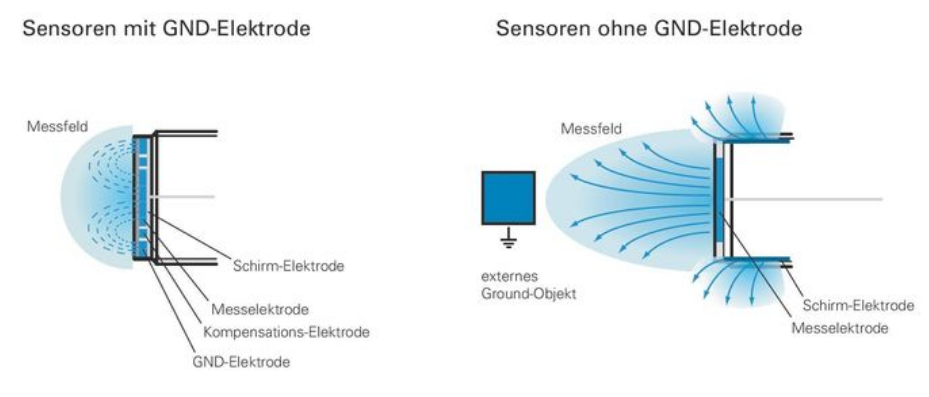
\includegraphics[scale=0.5]{fig/elektro/KapSensor.png}
    \caption{Arten von Kapazitiven Sensoren}
\end{figure}

\textbf{Sensoren mit GND-Elektrode} \\
Ein bündiger Einbau dieser Sensoren ist möglich, da sich ihr Messfeld von der Messelektrode zur integrierten GND-Elektrode ausbreitet.
Diese Variante eignet sich gut zur Detektion von nicht leitenden Materialien. \\

\textbf{Sensoren ohne GND-Elektrode} \\
Ein bündiges Einbauen dieser Art ist nicht vorteilhaft.
Eine integrierte GND-Elektrode ist nicht vorhanden, sie wird nämlich vom zu konstatierenden Objekt dargestellt.
Diese Bauform weist eine geringe Empfindlichkeit gegen Verschmutzung auf.
Für hohe Schaltabstände sind leitende und geerdete Gegenstände von Vorteil.

\subsubsection{Sensoren-Auswahl}

\begin{table}[h]
    \centering
    \begin{tabular}{|
    >{\columncolor[HTML]{FFFFFF}}l |
    >{\columncolor[HTML]{FFFFFF}}l |
    >{\columncolor[HTML]{FFFFFF}}l |
    >{\columncolor[HTML]{FFFFFF}}l |
    >{\columncolor[HTML]{FFFFFF}}l |}
        \hline
        & \textbf{Kapazitive Sensoren} & \textbf{Ultraschall-Sensoren} & \textbf{Optische Sensoren} \\ \hline
        Preis & gering & hoch & mittel    \\ \hline
        Platzbedarf & gering & gering & mittel   \\ \hline
        Genauigkeit & hoch & mittel & hoch        \\ \hline
    \end{tabular}
    \caption{Vergleich der Sensoreigenschaften}
\end{table}

Unsere Wahl fiel auf einen kapazitiven Sensor, da dieser für uns bereits für einen erschwinglichen Preis alles Nötige mit sich bringt: einen hohen Grad an Genauigkeit sowie einen geringen Platzbedarf.
Somit fiel unsere Wahl auf den LJC18A3, welcher mit einer Versorgungspannung von 6V bis 36V arbeitet und metallische und nichtmetallische Gegenstände in einem Schaltabstand von 1 bis 10mm erfassen kann.
Dieser Sensor konnte mit einem sehr geringen Preis in unseren Besitz gebracht werden und zeigte schon bei den ersten Tests, dass er alle Anforderungen erfüllte.

\subsection{Erfassung der Position des Motors}
\subsubsection{Endschalter}
Diese Realisierung umfasst einen Endschalter, welcher als Referenzpunkt vor jedem Mischvorgang angefahren wird, von diesem aus die benötigten Schritte aufgetragen werden.

\subsubsection{Lichtschranke}
Eine Lichtschranke würde, wie der Endschalter, am Anfang angefahren werden und so ebenfalls als Referenzpunkt fungieren.

\subsubsection{Varianten-Auswahl}
\begin{table}[h]
    \centering
    \begin{tabular}{|
    >{\columncolor[HTML]{FFFFFF}}l |
    >{\columncolor[HTML]{FFFFFF}}l |
    >{\columncolor[HTML]{FFFFFF}}l |
    >{\columncolor[HTML]{FFFFFF}}l |
    >{\columncolor[HTML]{FFFFFF}}l |}
        \hline
        & \textbf{Endschalter} & \textbf{Lichtschranke} \\ \hline
        Preis & sehr gering & mittel  \\ \hline
        Platzbedarf & sehr gering & mittel     \\ \hline
        Genauigkeit & mittel & hoch     \\ \hline
    \end{tabular}
    \caption{Vergleich der Erfassungsvarianten}
\end{table}

Unsere Wahl fiel auf den Endschalter, da dieser leicht in kürzester Zeit zu einem geringen Preis (je 1€) erworben werden konnte und ausreichend Genauigkeit mit sich bringt.

\subsection{Spannungsversorgung}
\subsubsection{Doppel-Schaltnetzteil mit zwei Ausgangsspannungspegeln}
Diese Variante wäre mit einem Netzteil zu realisieren, welches lediglich über einen Kaltgerätestecker mit einer Netzspannung von 230V \acs{AC} in Verbindung gebracht werden müsste,
um die Versorgung der Peripherie zu gewährleisten.
Sensoren, Schrittmotor und Hubmagneten würden über den 12V \acs{DC} Ausgang versorgt werden,
die Versorgung des Mikrocontrollers und des Raspberry Pi 3B+ würde über den 5V Ausgang des Schaltnetzteils realisiert werden.
Es müsste jedoch ein Pegelwandler zwischen dem Raspberry Pi und dem Mikrocontroller eingebaut werden, da die Spannungslogik des Raspberry auf 3.3V basiert und die des Mikrocontrollers auf 5V .

\begin{figure}[htb]
    \centering
    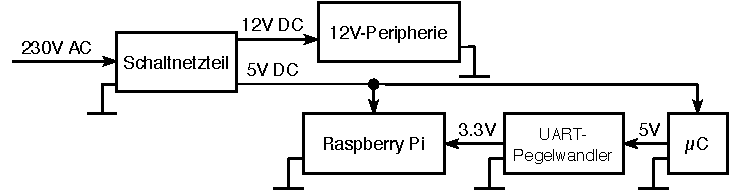
\includegraphics[scale=1,page=1]{fig/elektro/DoppelSchaltnetzteil.pdf}
    \caption{Blockschaltbild der Doppel-Schaltnetzteil-Anwendung}
\end{figure}

\subsubsection{Schaltnetzteil und Schaltregler}
Bei dieser Realisierung handelt es sich um ein mit 230V Wechselspannung versorgtes Netzteil, welches diese in ein 12V Gleichspannungssignal transferiert.
Jene 12V werden von jeglichen Aktoren und Sensoren genutzt.
Außerdem wird mithilfe der 12V ein Schaltregler mit Spannung versorgt, welcher die 5V Spannungsversorgung des Raspberry Pi bereitstellt.
Über den Erweiterungsstecker des Raspberry Pi wird folgend der Mikrocontroller mit 3.3V versorgt.

\begin{figure}[htb]
    \centering
    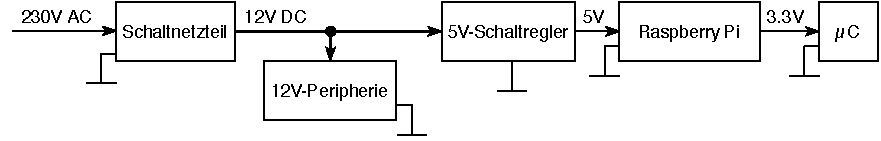
\includegraphics[scale=1,page=1]{fig/elektro/Schaltregler.pdf}
    \caption{Blockschaltbild der Schaltregler-Anwendung}
\end{figure}
\newpage
\subsubsection{Schaltnetzteil und Linearregler}
Bei dieser Alternative wird ein Schaltnetzteil mit 230V AC versorgt, welches ein 12V DC Signal am Ausgang bereitstellt.
Dieses wird für die 12V Peripherie genutzt sowie als Versorgung für einen Linearregler, welcher 12V zu 5V umwandelt.
Mit diesem Signal ist die Versorgung des Raspberry Pi bereitgestellt.
Die Versorgung des Mikrocontroller wird über zwei 3.3V Expansion Header Pins gewährleistet.

\begin{figure}[htb]
    \centering
    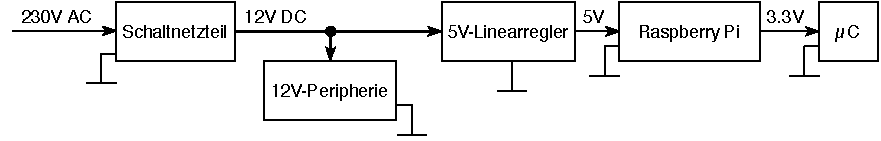
\includegraphics[scale=0.9,page=1]{fig/elektro/Linearregler.pdf}
    \caption{Blockschaltbild der Linearregler-Anwendung}
\end{figure}

\subsubsection{Auswahl der Spannungsversorgung}
\begin{table}[htbp]
    \centering
    \begin{tabular}{|
    >{\columncolor[HTML]{FFFFFF}}l |
    >{\columncolor[HTML]{FFFFFF}}l |
    >{\columncolor[HTML]{FFFFFF}}l |
    >{\columncolor[HTML]{FFFFFF}}l |
    >{\columncolor[HTML]{FFFFFF}}l |}
        \hline
        & \textbf{Doppel-Schaltnetzteil} & \textbf{\acs{SN} und Schaltregler} & \textbf{SN und Linearregler} \\ \hline
        Preis & hoch & mittel & gering    \\ \hline
        \multicolumn{1}{|l|}{\begin{tabular}[c]{@{}l@{}}
                                 Platzbedarf\\ und Gewicht
        \end{tabular}} & \multicolumn{1}{l|}{hoch} & \multicolumn{1}{l|}{gering} & \multicolumn{1}{l|}{gering} \\ \hline
        Bauteilbedarf & mittel & gering & sehr gering        \\ \hline
    \end{tabular}
    \caption{Vergleich der Spannungsversorgungsmodul-Attribute}
\end{table}

Unsere Wahl fiel auf die Variante des 12V Schaltnetzteils mit 5V Schaltregler, da diese für einen geringen Preis erhältlich ist
und einen ebenfalls geringen Bedarf an Platz und Bauteilen aufweist.
Außerdem bringt dieser gegenüber dem Linearregler eine höhere Effizienz sowie eine geringe Wärmeabstrahlung mit sich.
Den Mikrocontroller versorgen wir mit dem 3.3V Ausgang des Raspberry Pi 3B+.
Aufgrund der Tatsache, dass der Mikrocontroller mit einer Versorgung von 5V mit einer Logik von 5V arbeiten würde und somit ein Pegelwandler zu 3.3V nötig wäre, verwarfen wir die Idee diesen mit 5V zu versorgen.

\subsubsection{Leistungsbedarf}

Um die maximale Leistung des ATmega324PA zu berechnen, wird der maximal anfallende Ausgangsstrom bei unserer Verwendung herangezogen.
Dieser beträgt bei der Ansteuerung von zehn Ausgangspins etwa 60mA.
Multipliziert man diesen Strom mit der Versorgungsspannung von 3.3V, erhält man eine Leistung von 198mW.
Dieser Wert liegt unter der maximalen Leistung des µC von 660mW und ist somit zulässig.

\footfullcite{NCP1117-Datasheet}Um zu überprüfen, ob das 3.3V-Netz des Raspberry Pi auch im Stande dazu ist, diese Leistung zur Verfügung zu stellen, wird dessen Datenblatt herangezogen.
Auf dem Raspberry Pi 3B+ befindet sich ein Linearregler, welcher aus der 5V Versorgungsspannung eine 3.3V Spannung erzeugt.

\newpage

Die maximale Leistung ist somit von diesem abhängig und errechnet sich bei 50°C wie folgt:

\begin{align*}
    P_D &= \frac{T_{jmax} - (T_a + Sicherheit)}{R_{ja}}
\end{align*}
wobei
\begin{itemize}
    \item P\textsubscript{D} der auszurechnenden Verlustleistung,
    \item T\textsubscript{jmax} der maximalen Sperrschichttemperatur von 150°C,
    \item T\textsubscript{a} der Umgebungstemperatur und
    \item R\textsubscript{ja} dem Wärmewiderstand zwischen Sperrschicht und Umgebung von 160$\frac{^\circ C}{W}$ entspricht.
\end{itemize}

\begin{align*}
    P_D &= \frac{150^{\circ}C - (25^{\circ}C + 25)}{160 \frac{{}^{\circ}C}{W}} \\
    P_D &= 0.625W
\end{align*}

Der durchschnittliche Betrieb bei 25°C lässt folgende Leistung zu:
\begin{align*}
    P_D &= \frac{T_{jmax} - T_a}{R_{ja}} \\
    P_D &= \frac{150^{\circ}C - (25^{\circ}C)}{160\frac{{}^{\circ}C}{W}} \\
    P_D &= 0.78125W
\end{align*}

Am Linearregler fällt eine Dropout-Spannung von 1.7V ab.
Der maximale Strom kann somit ermittelt werden.

\begin{align*}
    P_{max} &= U_{DO} \cdot I_{max} \\
    I_{max} &= \frac{P_{max}}{U_{DO}} \\
    I_{max} &= \frac{0.625W}{1.7V} \\
    I_{max} &= 0.36765A
\end{align*}

Mit einem Abschlag von 250mA, welche zur Selbstversorgung des Raspberry Pi verwendet werden, steht ein Strom von 117.65mA an den 3.3V Expansion Header Pins zur Verfügung.
Das Leistungsmaximum der 3.3V-Pins beträgt somit 388.25mW .
(Im Betrieb bei 25°C liegt der maximale Strom bei 459.56mA und die maximale Leistung bei 691.55mW.)\\
Die maximalen Verluste des Linearreglers bei unserer Anwendung lassen sich auf folgende Weise kalkulieren:
\begin{align*}
    P_{V} &= U_{DO} \cdot I_{\mu Cmax} \\
    P_{V} &= 1.7V \cdot 60mA \\
    P_{V} &= 0.102W
\end{align*}

Der maximale Leistungsbedarf des Raspberry Pi liegt bei einem Strom von 750mA und mit Einbezug der Mikrocontrollerversorgung bei etwa 4W .

\subsection{Blockschaltbild der gesamten Elektronik}

\begin{figure}[hb]
    \centering
    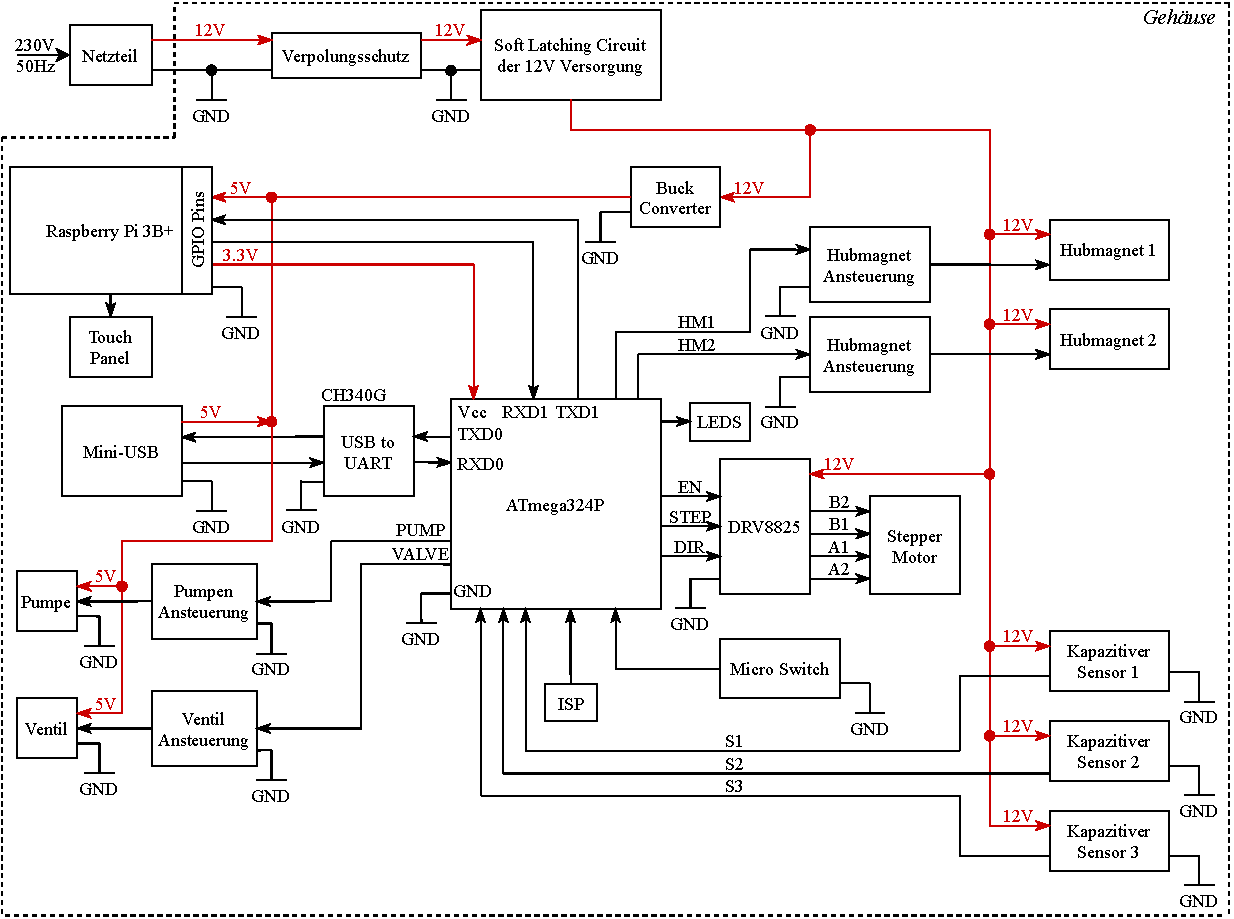
\includegraphics[scale=0.85,page=1]{fig/elektro/Blockschaltbild.pdf}
    \caption{Blockschaltbild der gesamten Elektronik}\label{fig:Blockschaltbild}
\end{figure}

\newpage

%/\-/\-/\-/\-/\-/\-/\-/\-/\-/\-/\-/\-/\-/\-/\-/\-/\-/\-/\-/\-/\-/\-/\-/\-/\-/\-/\-/\-/\-/\-/\-/\-/\-/\-/\-/\-/\-/\-/\-/\-/\-/\-/\-/\-/\-/\-/\-/\-/\-/\-/\-/\-/\-/\-/\-/\-/\-/\-/\-/\

\section{Schaltplan}

\subsection{Verpolungsschutz}
Da die Versorgungsspannung der elektrischen Baugruppen über eine Klemme eingespeist wird und eine Verwechslung der Anschlusspolaritäten nicht unwahrscheinlich ist,
vermag es einen Verpolungsschutz zu verwenden, um die dahinter gelegene Elektronik zu schützen.

\subsubsection{Verpolungsschutz mit einer Schottky-Diode}
\footfullcite{Verpolschutz}Die einfachste Methode diesen Schutz zu gewährleisten, ist über eine Schottkydiode.
Jedoch bringt diese Methode einen erheblichen Nachteil von einem dauerhaften Spannungsabfall von bis zu 0.3V im korrekten Betrieb mit sich.

\begin{figure}[ht]
    \centering
    \begin{circuitikz}[european, scale = 1.1]
        \draw (0,0) node[anchor=east] {-} to [short, o-*] (3,0);
        \draw (2,3) to[/tikz/circuitikz/bipoles/length=1cm, sD-, l=$D1$](4,3){};
        \draw (1,3) to [short, -o](0,3)node[anchor=east]{+};
        \draw (1,3) to [short, -o](6,3)node[anchor=west]{+};
        \draw (3,0) to [short, *-o](6,0)node[anchor=west]{-};
        \draw (4,0) to (3,0) node[rground]{};
        \draw (0,2.8) -- node[left] {$U_\mathrm{e}$}node[sloped,currarrow,pos=1] {}(0,0.2);
        \draw (6,2.8) -- node[right] {$U_\mathrm{a}$}node[sloped,currarrow,pos=1] {}(6,0.2);
    \end{circuitikz}
    \caption{Variante mithilfe einer Diode}
\end{figure}

\subsubsection{Verpolungsschutz mit einer Sicherung und einer Schottky-Diode}

Diese Realisierung bringt die Verwendung einer Sicherung und einer Schottky-Diode mit sich.

Bei verpolter anliegender Eingangsspannung brennt die Sicherung, bei ausreichendem,
von der Spannungsversorgung zur Verfügung gestelltem Strom, durch.
Jedoch entsteht die negative Tatsache einer verpolten Spannung von bis zu 0.3V, bis die Sicherung auslöst.

\begin{figure}[ht]
    \centering
    \begin{circuitikz}[european, scale = 1.1]
        \draw (0,0) node[anchor=east] {-} to [short, o-*] (3,0);
        \draw (1,3) to[R, l=$F1$](3,3){};
        \draw (4,0) to[/tikz/circuitikz/bipoles/length=1cm, sD-, l=$D1$, *-*](4,3){};
        \draw (1,3) to [short, -o](0,3)node[anchor=east]{+};
        \draw (1,3) to [short, -o](6,3)node[anchor=west]{+};
        \draw (3,0) to [short, *-o](6,0)node[anchor=west]{-};
        \draw (4,0) to (3,0) node[rground]{};
        \draw (4,0) to (4,2);
        \draw (0,2.8) -- node[left] {$U_\mathrm{e}$}node[sloped,currarrow,pos=1] {}(0,0.2);
        \draw (6,2.8) -- node[right] {$U_\mathrm{a}$}node[sloped,currarrow,pos=1] {}(6,0.2);
    \end{circuitikz}
    \caption{Zerstörerische Variante mithilfe einer Sicherung und einer Diode}
\end{figure}

\subsubsection{Verpolungsschutz mithilfe eines P-Kanal \acs{MOSFET}}

Der P-Kanal MOSFET leitet, wenn das Gate um U\textsubscript{GSth} negativer ist als der Spannungspegel anliegend am Source.
Das Anlegen einer korrekt gepolten Spannung am Eingang des MOSFET bewirkt ein Leiten der Bulk-Diode, sodass an der Source Spannung ankommt.
Da jene, an der Source anliegende Spannung weit über der U\textsubscript{GSth} liegt, leitet der MOSFET.
Die eingebaute Z-Diode begrenzt U\textsubscript{GS} auf einen für den MOSFET ungefährlichen Wert.
Die Tatsache, dass der MOSFET verkehrt herum leitet und der Drain somit ein höheres Potential als der Source hat, gilt als redondant, da es sich lediglich um einige Millivolt Unterschied handelt.
Sollte man eine verpolte Spannung am Eingang anlegen, sperrt die Bulk-Diode und der MOSFET gelangt nicht in den leitenden Zustand.
Bei Spannungen, die kleiner als die maximale U\textsubscript{GS} sind, kann die Z-Diode vernachlässigt werden.
In unserem Fall handelt es sich lediglich um eine anliegende Spannung von 12V, weshalb die Diode vernachlässigt werden kann und ein beinahe verlustfreier Betrieb möglich ist.

\begin{figure}[ht]
    \centering
    \begin{circuitikz}[european, scale = 1.2]
        \draw (0,0) node[anchor=east] {-} to [short, o-*] (2,0);
        \draw (2.6,4) to [short, *-](2.6,4.3) to [/tikz/circuitikz/bipoles/length=0.45cm,D-](3.4,4.3) to [short,-*](3.4,4){};
        \draw (3,4)node[pfet, rotate = 90 ](pfet){};
        \draw (pfet.G) node[anchor=east] {G};
        \draw (pfet.D) node[anchor=south] {S};
        \draw (pfet.S) node[anchor=south] {D};
        \draw (3.55,4.3)node[anchor=south]{Q1};
        \draw (3,0) to [R, l=$R1$, *-](3,3.3){};
        \draw (3,2.5) to [short, *-](4.2,2.5){};
        \draw (4.2,2.5) to [/tikz/circuitikz/bipoles/length=1cm,zD-, l=$D1$](4.2,4) to [short,-*](4.2,4) to (4.2,2.5){};
        \draw (3.225,4) to [short, -*](3.225,4);
        \draw (2.5,4) to [short, -o](0,4)node[anchor=east]{+};
        \draw (3,4) to [short, -o](6,4)node[anchor=west]{+};
        \draw (3,0) to [short, *-o](6,0)node[anchor=west]{-};
        \draw (3,0) to (2,0) node[rground]{};
        \draw (0,3.8) -- node[left] {$U_\mathrm{e}$}node[sloped,currarrow,pos=1] {}(0,0.2);
        \draw (6,3.8) -- node[right] {$U_\mathrm{a}$}node[sloped,currarrow,pos=1] {}(6,0.2);
    \end{circuitikz}
    \caption{Verpolungsschutz mit P-Kanal MOSFET für kleine Spannungen}
\end{figure}

Aufgrund der Vorteile des fast verlustlosen und wartungsarmen Betriebs entschieden wir uns für den Gebrauch der 3.Variante.

\newpage

\subsection{Soft-Latching-Circuit}

Eine Eingangsspannung von 12V, welche von einem Netzteil zur Verfügung gestellt wird, soll durch eine Tasterbetätigung durchgeschaltet werden und die Elektronik versorgen.
Diese Versorgung soll auch nach der Betätigung zur Verfügung stehen.
Sie soll lediglich mithilfe eines Touch-Panels über den \acs{RPI} gestoppt werden.
Außerdem soll ein korrektes Herunterfahren des RPI sichergestellt sein.

\subsubsection{Realisierte Variante mit einzelnem Taster}

Durch die Betätigung von S\textsubscript{1} fließt Strom durch R\textsubscript{2} und aktiviert somit den N-Kanal MOSFET Q\textsubscript{2}.
Dieser Feldeffekttransistor schaltet dadurch die am Drain anliegende Leitung auf Masse.
Das deshalb auf Masse gezogene Gate des P-Kanal MOSFET Q\textsubscript{1} lässt diesen durchschalten.
Über den Ausgang 12V\textsubscript{OUT} werden somit sämtliche 12V Sensoren, Aktoren und Elektronikkomponenten versorgt.
Das dadurch ebenfalls über R\textsubscript{3} versorgte Gate von Q\textsubscript{2} lässt die davon am Drain liegende Leitung auf Masse schalten,
welche die Versorgung der 12V Komponenten auch nach der Betätigung des S\textsubscript{1} bereitstellt.
Um diese Selbsthaltung wieder zu lösen, wird ein Signal über einen LCD eingelesen.
Der Raspberry wird heruntergefahren und über ein Watchdog-Signal erkennt dies der Mikrocontroller.
Dieser stellt somit ein digitales „High“ von 3.3V am Eingang U\textsubscript{UNLATCH} zur Verfügung.
Die Schottkydiode D\textsubscript{1} sorgt dafür, dass kein Strom zurück in den µC fließen kann und,
dass sich der aufgeladene Elektrolytkondensator nur über den Widerstand R\textsubscript{8} entlädt.
Das dadurch versorgte Gate von Q\textsubscript{3} schaltet die am Drain anliegende Leitung auf Masse.
Der dadurch deaktivierte Q\textsubscript{2} löst die Selbsthaltung und die Schaltung befindet sich wieder in ihrem Grundzustand.
Ein genaue Dimensionierung von C\textsubscript{1} und R\textsubscript{8} sorgen für ein ausreichend langes „High“ der Leitung,
sodass ein zuverlässiges Abschalten der 12V Ausgangsspannung bereitgestellt werden kann. \\

\begin{figure}[ht]
    \centering
    \begin{circuitikz}[european, scale = 1.15]
        \draw (0,0) node[anchor=east] {-} to [short, o-*] (2,0);

        \draw (1.7,7) to [R, l=$R1$, *-*](1.7,5.5) to (5.2,5.5){};
        \draw (3.5,7) to [R, l=$R2$, *-](3.5,5.5) to (3.5,4.8) to (3.2,4.8);
        \draw (3.2,4.2) to (3.5,4.2) to [short, -*](3.5,3);
        \draw (3.2,4.5)node[pushbuttonshape, rotate = 90]{};
        \draw (3,4.5) to (3,4.5)node[anchor=east]{S1};
        \draw (6,7) to (6,5.5);
        \draw (6,5.5)node[pfet, bodydiode]{};
        \draw (6,4) to [short, *-](7,4) to (7,7) to (10,7);
        \draw (7.5,7) to [R, l=$R6$, *-](7.5,5) to (7.5,5) node[rground]{};
        \draw (9,7) to [eC, l=$C2$, *-](9,5) to (9,5)node[rground]{};
        \draw (6,4.9) to (6,3) to [R, l_=$R3$](4,3) to (2,3);
        \draw (1.5,3)node[nfet, rotate=180](nfet1){};
        \draw (nfet1.G) node[anchor=south] {G};
        \draw (nfet1.D) node[anchor=east] {S};
        \draw (nfet1.S) node[anchor=east] {D};
        \draw (1.5,2.6) to [short, *-](1.2,2.6) to [/tikz/circuitikz/bipoles/length=0.45cm,D](1.2,3.4) to [short,-*](1.5,3.4){};
        \draw (1.5,0) to [short, *-](1.5,3);
        \draw (1.5,3.5) to (1.5, 5.5) to (1.7,5.5);
        \draw (2.6,0) to [R, l_=$R5$, *-*](2.6,3);
        \draw (8.3,2) to [short, o-](8.1,2) to [R, l_=$R7$](7.1,2) to [/tikz/circuitikz/bipoles/length=1cm, sD, l_=$D1$](6.1,2) to [eC, l=$C1$, *-*](6.1,0);
        \draw (6.2,2) to (4.8,2) to [R, l=$R8$, *-*](4.8,0);
        \draw (5,2) to (4.5,2);
        \draw (4,2) to [short, -*](4,0);
        \draw (4,2.5) to [short, -*](4,3);
        \draw (4,2)node[nfet, solderdot, rotate=180]{};
        \draw (4,1.6) to [short, *-](3.8,1.6) to [/tikz/circuitikz/bipoles/length=0.45cm,D](3.8,2.4) to [short,-*](4,2.4){};
        \draw (4,1.6) to [short, -*](4,1.775);
        \draw (1.5,2.775) to [short, -*](1.5,2.775);
        \draw (7.1,2) to (6.1,2);
        \draw (6,5.775) to [short, -*](6,5.725);
        \draw (6,5.1) to [short, -*](6,5.1);
        \draw (6,5.9) to [short, -*](6,5.9);
        \draw (8.3,0) to [short, -*](8.3,0);
        \draw (5.7,5.8) to (5.7,5.8)node[anchor=south]{Q1};
        \draw (1.9,3.3) to (1.9,3.3)node[anchor=south]{Q2};
        \draw (4.4,2.3) to (4.4,2.3)node[anchor=south]{Q3};
        \draw (8.3,2) to (8.3,2)node[anchor=west]{+};
        \draw (6,7) to [short, -o](0,7)node[anchor=east]{+};
        \draw (9,7) to [short, -o](10,7)node[anchor=west]{$12V_\mathrm{OUT}$};
        \draw (3,0) to [short, -o](10,0)node[anchor=west]{0V};
        \draw (3,0) to (2,0) node[rground]{};
        \draw (0,6.8) -- node[left] {$U_\mathrm{e}$}node[sloped,currarrow,pos=1] {}(0,0.2);
        \draw (10,6.8) -- node[right] {$U_\mathrm{a}$}node[sloped,currarrow,pos=1] {}(10,0.2);
        \draw (8.3,1.8) -- node[right] {$U_\mathrm{UNLATCH}$}node[sloped,currarrow,pos=1] {}(8.3,0.2);
    \end{circuitikz}
    \caption{12V Soft-Latching Circuit}
    \label{fig:SoftLatchingCircuit}
\end{figure}

\subsubsection{Dimensionierung der UNLATCH - Komponenten}

\begin{figure}[ht]
    \centering
    \begin{circuitikz}[european, scale = 1.2]
        \draw (1.5,2) to [/tikz/circuitikz/bipoles/length=1cm, sD-, l=$D1$](2.5,2);
        \draw (-0.5,2) to (0.5,2) to [R, l=$R7$](1.5,2);
        \draw (2.5,2) to (3,2) to [eC, l=$C1$, *-*](3,0);
        \draw (3,2) to (4.5,2) to [R, l=$R8$, *-*](4.5,0) to (2.05,0);
        \draw (4.5,2) to (4.8,2);
        \draw (5.5,2)node[nfet]{};
        \draw (5.5,2) to [short, -*](5.5,1.775) to (5.5,0) to (4.5,0);
        \draw (-1.25,2.5)node[anchor=north]{µC};
        \draw (-1.25,1.5) to (-1.25,0) to (2,0);
        \draw (-2,1.5) to (-0.5,1.5) to (-0.5,3) to (-2,3) to (-2,1.5);
        \draw (2,0) to [short, -*](2,0) node[rground]{};
        \draw (5.5,2.3) to (5.5,3)node[vcc]{};
        \draw (-1.25,3) to (-1.25,3)node[vcc]{Vcc};
        \draw (0,1.8) -- node[right] {$U_\mathrm{UNLATCH}$}node[sloped,currarrow,pos=1] {}(0,0.2);
    \end{circuitikz}
    \caption{Schaltung zum Aufheben der Selbsthaltung}
    \label{fig:UNLATCH}
\end{figure}

Um Berechnungen von verschiedensten Werten vorzunehmen, wird Gebrauch von einigen grundlegenden Formeln der Elektrotechnik gemacht:

\begin{align}
    R_{ges} &= \frac{R1 \cdot R2}{R1+R2} \\
    u_C(t) &= 1(t) \cdot (1-e^{\frac{-1}{\tau}}) \\
    u_c(t) &= 1(t) \cdot e^{\frac{-1}{\tau}} \\
    \sum_{k=1}^n U_k &= 0 \\
    \tau &= R \cdot C
\end{align}

Vereinfacht man die in \autoref{fig:UNLATCH} zu sehende Schaltung, erhält man folgendes Ersatzschaltbild:

\begin{figure}[ht]
    \centering
    \begin{circuitikz}[european, scale = 1]
        \draw (0,2) to [V_=$3.3V$](0,0);
        \draw (0,2) to [R, l=$R7$](2,2) to [V=$0.3V$](4,2);
        \draw (4,2) to [R, l=$R8$, *-*](4,0);
        \draw (4,2) to (5,2);
        \draw (0,0) to (5,0);
        \draw (2.75,0) to [short, -*](2.75,0) node[rground]{};
        \draw [line width = 1.2](4.9,0.1) to (5.1,-0.1);
        \draw [line width = 1.2](4.9,-0.1) to (5.1,0.1);
        \draw [line width = 1.2](4.9,2.1) to (5.1,1.9);
        \draw [line width = 1.2](4.9,1.9) to (5.1,2.1);
    \end{circuitikz}
    \caption{Ersatzschaltbild des UNLATCH-Schaltung}
\end{figure}

Dies hilft uns, den Gesamtwiderstand der Schaltung auszurechnen.
Mann kann das Ersatzschaltbild in weiterer Folge zusammenfassen, womit der Betrag der Zeitkonstante $\tau$ berechnet werden kann.

\newpage
Als Bauteilwerte erstellten wir folgende Annahmen:

\begin{itemize}
    \item R7 = 560$\Omega$, R8 = 100k$\Omega$, C1 = 100$\mu$F
\end{itemize}

\begin{figure}[ht]
    \centering
    \begin{circuitikz}[european, scale = 1.1]
        \draw (0,2) to [V_=$3V$](0,0);
        \draw (0,2) to [R, l=$R7||R8$](2,2);
        \draw (2,2) to (4,2) to [C, l=$C1$](4,0);
        \draw (0,0) to (4,0);
        \draw (2.75,0) to [short, -*](2.75,0) node[rground]{};
        \draw [line width = 1.2](1.9,2.1) to (2.1,1.9);
        \draw [line width = 1.2](1.9,1.9) to (2.1,2.1);
        \draw [line width = 1.2](1.9,0.1) to (2.1,-0.1);
        \draw [line width = 1.2](1.9,-0.1) to (2.1,0.1);
        \draw (2.75,1.8) -- node[left] {$U_\mathrm{X}$}node[sloped,currarrow,pos=1] {}(2.75,0.3);
    \end{circuitikz}
    \caption{Vereinfachung des Ersatzschaltbildes}
\end{figure}

\begin{align*}
    \tau &= (\frac{R7 \cdot R8}{R7 + R8}) \cdot C1 \\
    \tau &= (\frac{560\Omega \cdot 100k\Omega}{560\Omega + 100k\Omega}) \cdot 100\mu F \\
    \tau &= 556.8815\Omega \cdot 100\mu F \\
    \tau &= 55.688ms
\end{align*}

\begin{align*}
    U_X &= 3V \cdot \frac{R8}{R7+R8} \\
    U_X &= 3V \cdot \frac{100000\Omega}{560\Omega+100000\Omega} \\
    U_X &= 2.983V
\end{align*}

Die Thresholdvoltage der von uns ausgewählten MOSFETs liegt bei 1V .
Über das Umformen der Gleichung 2.2 kann die Zeit bis zur Schaltschwelle ermittelt werden.

\begin{align*}
    u_{c}(t) &= U_X \cdot (1 - e^{\frac{-t}{\tau}}) \\
    \frac{u_{c}}{U_X} &= 1 - e^{\frac{-t}{\tau}} \\
    1 - \frac{u_{c}}{U_X} &= e^{\frac{-t}{\tau}} \\
    ln(1 - \frac{u_{c}}{U_X}) &= \frac{-t}{\tau} \\
    ln(1 - \frac{u_{c}}{U_X}) \cdot \tau &= -t \\
    -t &= ln(1 - \frac{1V}{2.983V}) \cdot 0.055688s \\
    t &= 22.736ms
\end{align*}

Sollte der Mikrocontroller die Versorgung aller Peripheriebausteine unterbrechen, so schwindet auch die Versorgung des µC .
Über die Annahme, dass dies nicht innerhalb von 100ms passiert, wird zunächst die Spannung nach 100ms berechnet.

\begin{align*}
    u_{c}(t) &= U_X \cdot (1 - e^{\frac{-t}{\tau}}) \\
    u_{c}(t) &= 2.983V \cdot (1 - e^{\frac{-0.1s}{0.055688s}}) \\
    u_{c}(t) &= 2.488V
\end{align*}

Der aktivierte MOSFET soll mindestens für eine Zeit von 7s aktiviert sein, um ein möglichst sicheres Abschalten der Versorgung zu gewährleisten.
Über diese Anforderung wird die Spannung des Kondensators nach 7 Sekunden berechnet. \\

\begin{figure}[ht]
    \centering
    \begin{circuitikz}[european, scale = 1.1]
        \draw (4,2) to [C, l=$C1$, *-*](4,0);
        \draw (5.5,2) to [R, l=$R8$, *-](5.5,0);
        \draw (2,0) to (5.5,0);
        \draw (2,2) to (6.5,2);
        \draw (2.75,0) to [short, -*](2.75,0) node[rground]{};
        \draw [line width = 1.2](1.9,2.1) to (2.1,1.9);
        \draw [line width = 1.2](1.9,1.9) to (2.1,2.1);
        \draw [line width = 1.2](6.4,2.1) to (6.6,1.9);
        \draw [line width = 1.2](6.4,1.9) to (6.6,2.1);
        \draw [line width = 1.2](1.9,0.1) to (2.1,-0.1);
        \draw [line width = 1.2](1.9,-0.1) to (2.1,0.1);
        \draw (2.75,1.8) -- node[left] {$U_\mathrm{X}$}node[sloped,currarrow,pos=1] {}(2.75,0.3);
    \end{circuitikz}
    \caption{Ersatzschaltbild des Entladezyklus}
\end{figure}

\begin{align*}
    u_{c}(t) &= U_X \cdot e^{\frac{-t}{\tau}} \\
    u_{c}(t) &= 2.488V \cdot e^{\frac{-7s}{100k\Omega \cdot 100\mu F}} \\
    u_{c}(t) &= 1.235V
\end{align*}

Die Berechnung zeigt, dass nach einer Zeit von 7 Sekunden, die Spannung anliegend am Gate des MOSFET noch immer weit über der Theshold-Voltage liegt.
(Die Schwelle von 1V wird nach 9.115 Sekunden erreicht.)

\newpage
\subsubsection{Andere Variante}
\footfullcite{EEVblog-262-Worlds-Simplest-Soft-Latching-Power-Switch-Circuit}Die folgende Variante kam ebenfalls im Laufe der Diplomarbeit auf.

Sobald S\textsubscript{1} betätigt wird fließt Strom durch den Widerstand R\textsubscript{2}, wodurch der Bipolartransistor Q\textsubscript{2}
die am Collector anliegende Leitung auf Masse schaltet.
Das dadurch auf Masse gezogene Gate des P-Kanal MOSFET lässt diesen durchschalten und eine Ausgangsspannung von 12V ist verfügbar.
Der durch den Widerstand R\textsubscript{3} fließende Strom sorgt für ein Durchschalten des npn-Transistors, auch wenn der Taster S1 nicht mehr gedrückt ist.

Ein Betätigen des Tasters S\textsubscript{2} hat zur Folge, dass die Basis des Transistors Q\textsubscript{2} auf Masse gezogen wird.
Dies hat zur Folge einen positiven Pegel am Gate des MOSFETs zu erzeugen, welcher diesen sperren lässt.
Somit kann am Ausgang keine Spannung vorgefunden werden.
Um ein floatendes Gate von Q\textsubscript{1} zu vermeiden, ist der Widerstand R\textsubscript{1} vom Drain auf das Gate geschaltet.

\begin{figure}[ht]
    \centering
    \begin{circuitikz}[european, scale = 1]
        \draw (0,0) node[anchor=east] {-} to [short, o-*] (2,0);
        \draw (2,6)node[pfet,bodydiode, rotate = 90]{};
        \draw (1,6) to [R, l=$R1$, *-](1,4) to (2,4) to (2,5.2);
        \draw (2,4) to [short, *-](2,2.5);
        \draw (2.5,6) to (5,6);
        \draw (0.5,6) to [short, *-](0.5,7) to (6,7) to (6,5) to [R,l=$R2$](6,3) to (6,2.5) to (5.8,2.5);
        \draw (5,2) to (5,1.5) to (5.15,1.5);
        \draw (5.5,1.5)node[pushbuttonshape]{};
        \draw (5.5,2.5)node[pushbuttonshape]{};
        \draw (5.9,1.5) to (6,1.5) to (6,0) to (2,0);
        \draw (5.1,2.5) to (5,2.5) to [short,-*](5,2);
        \draw (3.5,6) to [R, l=$R3$, *-*](3.5,2) to (5,2);
        \draw (4,2) to (2.5,2);
        \draw (2,1.5) to (2,0);
        \draw (1.9,2) to (1.9,2)node[anchor=east]{Q2};
        \draw (1.4,6.8) to (1.4,6.8)node[anchor=north]{Q1};
        \draw (5.5,2.3) to (5.5,2.3)node[anchor=north]{S2};
        \draw (5.5,3.3) to (5.5,3.3)node[anchor=north]{S1};
        \draw (2,2)node[npn, xscale = -1](npn){};
        \draw (npn.E) node[left]{E};
        \draw (npn.C) node[left]{C};
        \draw (npn.B) node[above]{B};
        \draw (2,6) to (1.775,6) to [short, *-o](0,6)node[anchor=east]{+};
        \draw (4,6) to [short, -o](5,6)node[anchor=west]{+};
        \draw (5,4) to (5,4)node[anchor=west]{-};
        \draw (3,0) to (2,0) node[rground]{};
        \draw (5,4) to [short, o-o](5,4)to(5,3.9) node[rground]{};
        \draw (0,5.8) -- node[left] {$U_\mathrm{e}$}node[sloped,currarrow,pos=1] {}(0,0.2);
        \draw (5,5.8) -- node[right] {$U_\mathrm{a}$}node[sloped,currarrow,pos=1] {}(5,4.2);
    \end{circuitikz}
    \caption{Realisierung einer Selbsthaltung mit zwei Tastern}
\end{figure}

Diese Variante wurde letztendlich verworfen, da wir uns dazu entschieden haben, nur einen Schalter zu verwenden, wessen Funktion das Einschalten der 12V sein soll.
Außerdem soll ein sicheres Herunterfahren des Raspberry Pi gewährleistet sein, welches diese Schaltung nicht bereitstellen kann.

\newpage

\subsection{DC/DC Wandler}

\footfullcite{LM2576-Datasheet}Als Buck-Converter wählten wir den LM2576-5.0 aus.
Mit diesem ist es möglich eine Eingangsspannung von 7V bis 40V zu einer Spannung von 5V mit einem Strom von maximal 3A umzuwandeln.
Weitere Kriterien, die unsere Wahl befürworteten, waren die niedrige Anzahl von nur vier zusätzlichen Bauteilen, der hohe maximale Ausgangsstrom sowie die hohe Effizienz.

\subsubsection{Beschaltung}

\begin{figure}[ht]
    \centering
    \begin{circuitikz}[european, scale = 1.2]
        \draw (0,0) node[anchor=east] {-} to [short, o-*] (1,0);
        \draw (1.5,5) to [eC, l=$C1$, *-*](1.5,0);
        \draw (8.5,5) to [eC, l=$C2$, *-*](8.5,0);
        \draw (6.5,0) to [/tikz/circuitikz/bipoles/length=1cm, sD, l_=$D1$, *-*](6.5,5) to (6.5,0);
        \draw [line width=1.5pt](3,4) to (3,6) to (5.5,6) to (5.5,4) to (3,4);
        \draw (5.5,5.5) to (8.5,5.5) to (8.5,5) to [short,i=$I_{LOAD}$](10,5);
        \draw (5.5,5) to (6.5,5);
        \draw (6.5,5) to [L, l_=$L1$](8.5,5);
        \draw (3.5,4) to [short, -*](3.5,0);
        \draw (5,4) to [short, -*](5,0);
        \draw (4.25,5.25) to (4.25,5.25)node[anchor=north]{LM2576-5.0};
        \draw (3.1,5.2) to (3.1,5.2)node[anchor=east]{VIN};
        \draw (3.5,3.8) to (3.5,3.8)node[anchor=east]{GND};
        \draw (5.1,3.8) to (5.1,3.8)node[anchor=east]{ON/OFF};
        \draw (6.6,5.2) to (6.6,5.2)node[anchor=east]{VOUT};
        \draw (6.1,5.7) to (6.1,5.7)node[anchor=east]{FB};
        \draw (3,5) to [short, -o](0,5)node[anchor=east]{+};
        \draw (8.5,5) to [short, -o](10,5)node[anchor=west]{+};
        \draw (3,0) to [short, -o](10,0)node[anchor=west]{-};
        \draw (3,0) to (1,0) node[rground]{};
        \draw (0,4.8) -- node[left] {$V_\mathrm{IN}$}node[sloped,currarrow,pos=1] {}(0,0.2);
        \draw (10,4.8) -- node[right] {$V_\mathrm{OUT}$}node[sloped,currarrow,pos=1] {}(10,0.2);
    \end{circuitikz}
    \caption{Beschaltung des LM2576-5.0}
\end{figure}

\subsubsection{Kühlkörperberechnung}

Um die Notwendigkeit eines Kühlkörpers zu berechnen, werden Formeln der Datenblätter zur Berechnung angewandt.
Um die Verlustleistung zu berechnen, wird folgende Formel angewandt.

\begin{equation}
    P_D = V_{IN} \cdot I_Q + \frac{V_{OUT}}{V_{IN}} \cdot I_{LOAD} \cdot V_{SAT}
\end{equation}
wobei
\begin{itemize}
    \item P\textsubscript{D} der auszurechnenden Verlustleistung,
    \item V\textsubscript{IN} der Eingangsspannung,
    \item I\textsubscript{Q} dem Ruhestrom (siehe Datenblatt),
    \item V\textsubscript{OUT} der regulierten Ausgangsspannung,
    \item I\textsubscript{LOAD} dem Laststrom und V\textsubscript{SAT} der Sättigungsspannung (siehe Datenblatt) entspricht.
\end{itemize}

Setzen wir nun die bei unserer Anwendung durchschnittlich anfallenden Werte ein, erhalten wir folgendes Ergebnis:
\begin{align*}
    P_D &= 12V \cdot 0.015A + \frac{5V}{12V} \cdot 1.5A \cdot 1.2V \\
    P_D &= 0.93W
\end{align*}

Die daraus folgende Sperrschichtübergangstemperatur lässt sich mit dieser Formel berechnen:
\begin{align}
    T_j &= P_D \cdot R_{ja} + T_A\\
    T_j &= 0.93W \cdot 70\frac{{}^{\circ}C}{W} + 25^{\circ}C \notag \\
    T_j &= 90.1^{\circ}C \notag
\end{align}

Da sich die zulässige maximale Sperrschichttemperatur bei 125°C liegt, lässt es sich auf einen zulässigen Dauerbetrieb schließen.\\
Um jedoch Gewissheit zu erlangen, ob sommerliche Extremtemperaturen im Gehäuse (50°C) keinen schädigenden Einfluss haben würden, ist dieser Fall ebenfalls zu berechnen.
\begin{align*}
    T_j &= P_D \cdot R_{ja} + T_A\\
    T_j &= 0.93W \cdot 70\frac{{}^{\circ}C}{W} + 50^{\circ}C \\
    T_j &= 115.1^{\circ}C
\end{align*}

Ein Betrieb bei derartigen Temperaturen ist somit zulässig.
In Anbetracht, dass derartige Hitze die Langlebigkeit begrenzen würde, ist es dennoch ratsam, einen Kühlkörper zu verwenden.

\subsection{Raspberry Pi 3B+}

Als Basis für unsere Human Machine Interface wählten wir einen Raspberry Pi 3B+ aus.
Die Begründung dieser Wahl befindet sich im Infortmatik-Teil dieser Diplomarbeit.
Dieser hat die Aufgabe den Mikroprozessor ATmega324PA mit 3.3V zu versorgen sowie über das Touchpanel eingelesene Information mit dem Mikroprozessor auszutauschen.

\subsubsection{Watchdog}

Als Funktion der Ausfallerkennung implementierten wir eine Watchdog-Verbindung zwischen dem Raspberry Pi und dem Mikrocontroller.
So kann bei einem Ausfall dennoch eine sicheres Herunterfahren sowie ein sicheres Lesen beziehungsweise Schreiben einer Datei gewährleistet werden.

\subsection{Beschaltung des ATmega324PA}

\footfullcite{Datasheet-ATmega324PA}Um den Mikrocontroller zu versorgen, wurde an allen VCC-Pins und am AVCC-Pin eine Verbindung zum 3.3V Ausgang des Raspberry Pi vorgesehen.
Um die Versorgungsspannung von 3.3V zu glätten, wurde an allen 4 Versorgungspins je ein Kondensator mit 100nF vorgesehen.
An jeglichen GND Anschlüssen des Mikrocontrollers wurde eine Leitung gegen Masse implementiert.

Um die interne Referenzspannung zu glätten, wurde wie im Datenblatt empfohlen, ein 100nF Kondensator am Pin AREF implementiert.
Laut dem zugehörigen Datenblatt ist bei einer Versorgungspannung von 3.3V ein Quarz mit einer Taktfrequenz von 0 bis 13.3MHz zu arbeiten.
Aufgrund unserer Entscheidung, den Mikrocontroller mit einem 10MHz Quarz zu betreiben, waren zwei Kondensatoren mit einem Wert von 12 bis 22pF zu wählen.
Diese haben den Nutzen, den Quarzoszillator gut anschwingen und stabil schwingen zu lassen.
Der RESET-Pin setzt bei einem LOW-Pegel-Signal den µC zurück.
Um dies im Grundzustand zu unterbinden, wird ein Pull-Up Widerstand von 10kOhm implementiert.
Parallel zu diesem wurde eine externe Diode zum Schutz vor Überspannungen vorgesehen.
Um den RESET-Pin gegen Masse schalten zu können, wurde ein Taster implementiert.
Über den Data-Terminal-Ready Pin des USB-UART-Converters und dessen Jumper-Pad oder die ISP-Schnittstelle ist es jedoch ebenfalls möglich, den ATmega324PA zu resetten.
Parallel zum Taster wurde ein Kondensator vorgesehen, welcher als Prevention gegen Spikes und für ein längeres, definiertes Bestehen des µC im Reset-Zustand dient.

\begin{figure}[ht]
    \centering
    \begin{circuitikz}[european, scale = 1.1]
        \draw [line width=1.5pt](5,0) to (8.5,0) to (8.5,5) to (5,5) to (5,0);

        %AREF
        \draw (7.9,2) to (7.9,2)node[anchor=north]{AREF};
        \draw (8.5,1.75) to (9.5,1.75) to [C, l=$C9$](9.5,0) to (9.5,0) node[rground]{};

        %ISP
        \draw (8.5,2.5) to (10,2.5);
        \draw (8.5,3) to (10,3);
        \draw (8.5,3.5) to (10,3.5);
        \draw (7.9,2.7) to (7.9,2.7)node[anchor=north]{MOSI};
        \draw (7.9,3.2) to (7.9,3.2)node[anchor=north]{MISO};
        \draw (7.9,3.7) to (7.9,3.7)node[anchor=north]{SCK};

        \draw [line width=1.5pt](10,2) to (10,4) to (11.5,4) to (11.5,2) to (10,2);
        \draw (11.5,2.5) to (12,2.5) to (12,2)node[rground]{};
        \draw (11.5,3.5) to (12,3.5) to (12,4)node[vcc]{+3.3V};
        \draw (11.5,3) to [short,-o](12,3);
        \draw (13.6,3)to (13.6,3)node[anchor=east]{ISP-RST};
        \draw (11.8,4.3)node[anchor=east]{ISP-Header};

        %Quarz
        \draw (5.65,2.8) to (5.65,2.8)node[anchor=north]{XTAL2};
        \draw (5.65,1.2) to (5.65,1.2)node[anchor=north]{XTAL1};
        \draw (5,2.6) to (3,2.6);
        \draw (5,1) to (3,1);
        \draw (4,2.6) to [PZ, l_=$Y1$, *-*](4,1);
        \draw (3,1) to [C, l=$C8$](1.5,1);
        \draw (3,2.6) to [C, l=$C7$](1.5,2.6);
        \draw (1.5,1) to (1.5,2.6);
        \draw (1.5,1.8) to [short, *-](0.5,1.8) to (0.5,1)node[rground]{};

        %RESET
        \draw (5.65,4) to (5.65,4)node[anchor=north]{RESET};
        \draw [line width=1.2pt](5.1,3.95) to (6.2,3.95);
        \draw (5,3.7) to (3,3.7) to (3,6) to [R, l=$R1$](3,7.5) to (3,8)node[vcc]{+3.3V};
        \draw (3,6) to [short, *-](4,6) to [/tikz/circuitikz/bipoles/length=1cm, sD, l_=$D1$](4,7.5) to  [short,-*](3,7.5);
        \draw (4,7.5) to (4,6);
        \draw (3,5.5) to [short,*-o](3.5,5.5)node[anchor=west]{ISP-RST};
        \draw (3,5) to [short, *-o](2,5);
        \draw (1.5,5) to [short, o-](0.5,5) to [C, l=$C5$](0.5,6.5) to [short, -o](0,6.5)node[anchor=east]{DTR-USB};
        \draw [line width=1.2pt](-1,6.75) to (-1.8,6.75);
        \draw (-0.5,5.3) to (-0.5,5.3)node[anchor=west]{10n};
        \draw (3,4.5) to [short,*-](-1,4.5) to [C=100n, l_=$C6$](-1,1.5) to (-1,1.5)node[rground]{};
        \draw (-2,2.6) to (-2,2.6)node[anchor=west]{100n};
        \draw (3,4) to [short, *-](2.15,4);
        \draw (1.8,4)node[pushbuttonshape]{};
        \draw (1.48,4) to [short,o-](0.5,4) to (0.5,3.5)node[rground]{};
        \draw (1.825,4) to (1.825,4)node[anchor=north]{S1};

        \draw (1.825,5.7) to (1.825,5.7)node[anchor=north]{Jumper};

        %VCC und GND
        \draw (5.4,5) to (5.4,5)node[anchor=north]{VCC};
        \draw (6.2,5) to (6.2,5)node[anchor=north]{VCC};
        \draw (7,5) to (7,5)node[anchor=north]{VCC};
        \draw (7.9,5) to (7.9,5)node[anchor=north]{AVCC};
        \draw (5.45,0.5) to (5.45,0.5)node[anchor=north]{GND};
        \draw (6.3,0.5) to (6.3,0.5)node[anchor=north]{GND};
        \draw (7.15,0.5) to (7.15,0.5)node[anchor=north]{GND};
        \draw (8,0.5) to (8,0.5)node[anchor=north]{GND};

        \draw (5.4,7.5) to [short, *-*](6.2,7.5) to [short,-*](7.9,7.5) to [short,-*](9.6,7.5) to(11.2,7.5);
        \draw (6.2,6) to [short,-*](7.9,6) to [short,-*](9.6,6) to [short,-*](11.2,6) to (11.2,5.5)node[rground]{};
        \draw (6.2,7.5) to [C, l=$C1$](6.2,6);
        \draw (7.9,7.5) to [C, l=$C2$](7.9,6);
        \draw (9.6,7.5) to [C, l=$C3$](9.6,6);
        \draw (11.2,7.5) to [C, l=$C4$](11.2,6);


        \draw (5.4,8) to (5.4,5);
        \draw (5.4,5.5) to [short, *-*] (6.2,5.5) to [short, *-*] (7,5.5) to (7.9,5.5);
        \draw (6.2,5.5) to (6.2,5);
        \draw (7,5.5) to (7,5);
        \draw (7.9,5.5) to (7.9,5);

        \draw (5.5,-0.4) to [short, *-*] (6.3,-0.4) to [short, *-*] (7.1,-0.4) to (8,-0.4);
        \draw (6.3,-0.4) to (6.3,0);
        \draw (7.1,-0.4) to (7.1,0);
        \draw (8,-0.4) to (8,0);

        %Beschriftungen
        \draw (9.2,5.6) to (9.2,5.6)node[anchor=north]{ATmega324PA};
        \draw (5.4,8)node[vcc]{+3.3V};
        \draw (5.5,0) to (5.5,-0.5) node[rground]{};
    \end{circuitikz}
    \caption{Beschaltung des ATmega324PA}
\end{figure}

\subsection{DRV8825-Schrittmotortreiber}

\footfullcite{DRV8825-Datasheet}Dieses Modul ist dafür ausgelegt, bipolare Schrittmotoren anzusteuern.
Der DRV8825 besitzt zwei H-Brücken-Treiber und einen Microstepping Indexer.
Um die Motorwindungen anzusteuern, sind die Ausgangsblöcke des Treibers als volle N-Kanal Leistung-MOSFET H-Brücken realisiert.
Dem DRV8825 ist es möglich einen Ausgangsstrom von bis zu 2.5A bei geeigneter Kühlung zu treiben.

\subsubsection{Datenblattwerte}

\begin{minipage}{.6\textwidth}
    \begin{itemize}
        \item Minimale Betriebsspannung 8.2V
        \item Maximale Betriebsspannung 47V
        \item Maximaler Strom per Phase 1.5A (2.5A*)
        \item Minimale Steuerspannung 2.2V
        \item Maximale Steuerspannung 5.25V
        \item Dimensionen 15.5mm x 20.5mm
    \end{itemize}
    * nur bei ausreichender Kühlung möglich
\end{minipage}
\begin{minipage}{.4\textwidth}
    \centering
    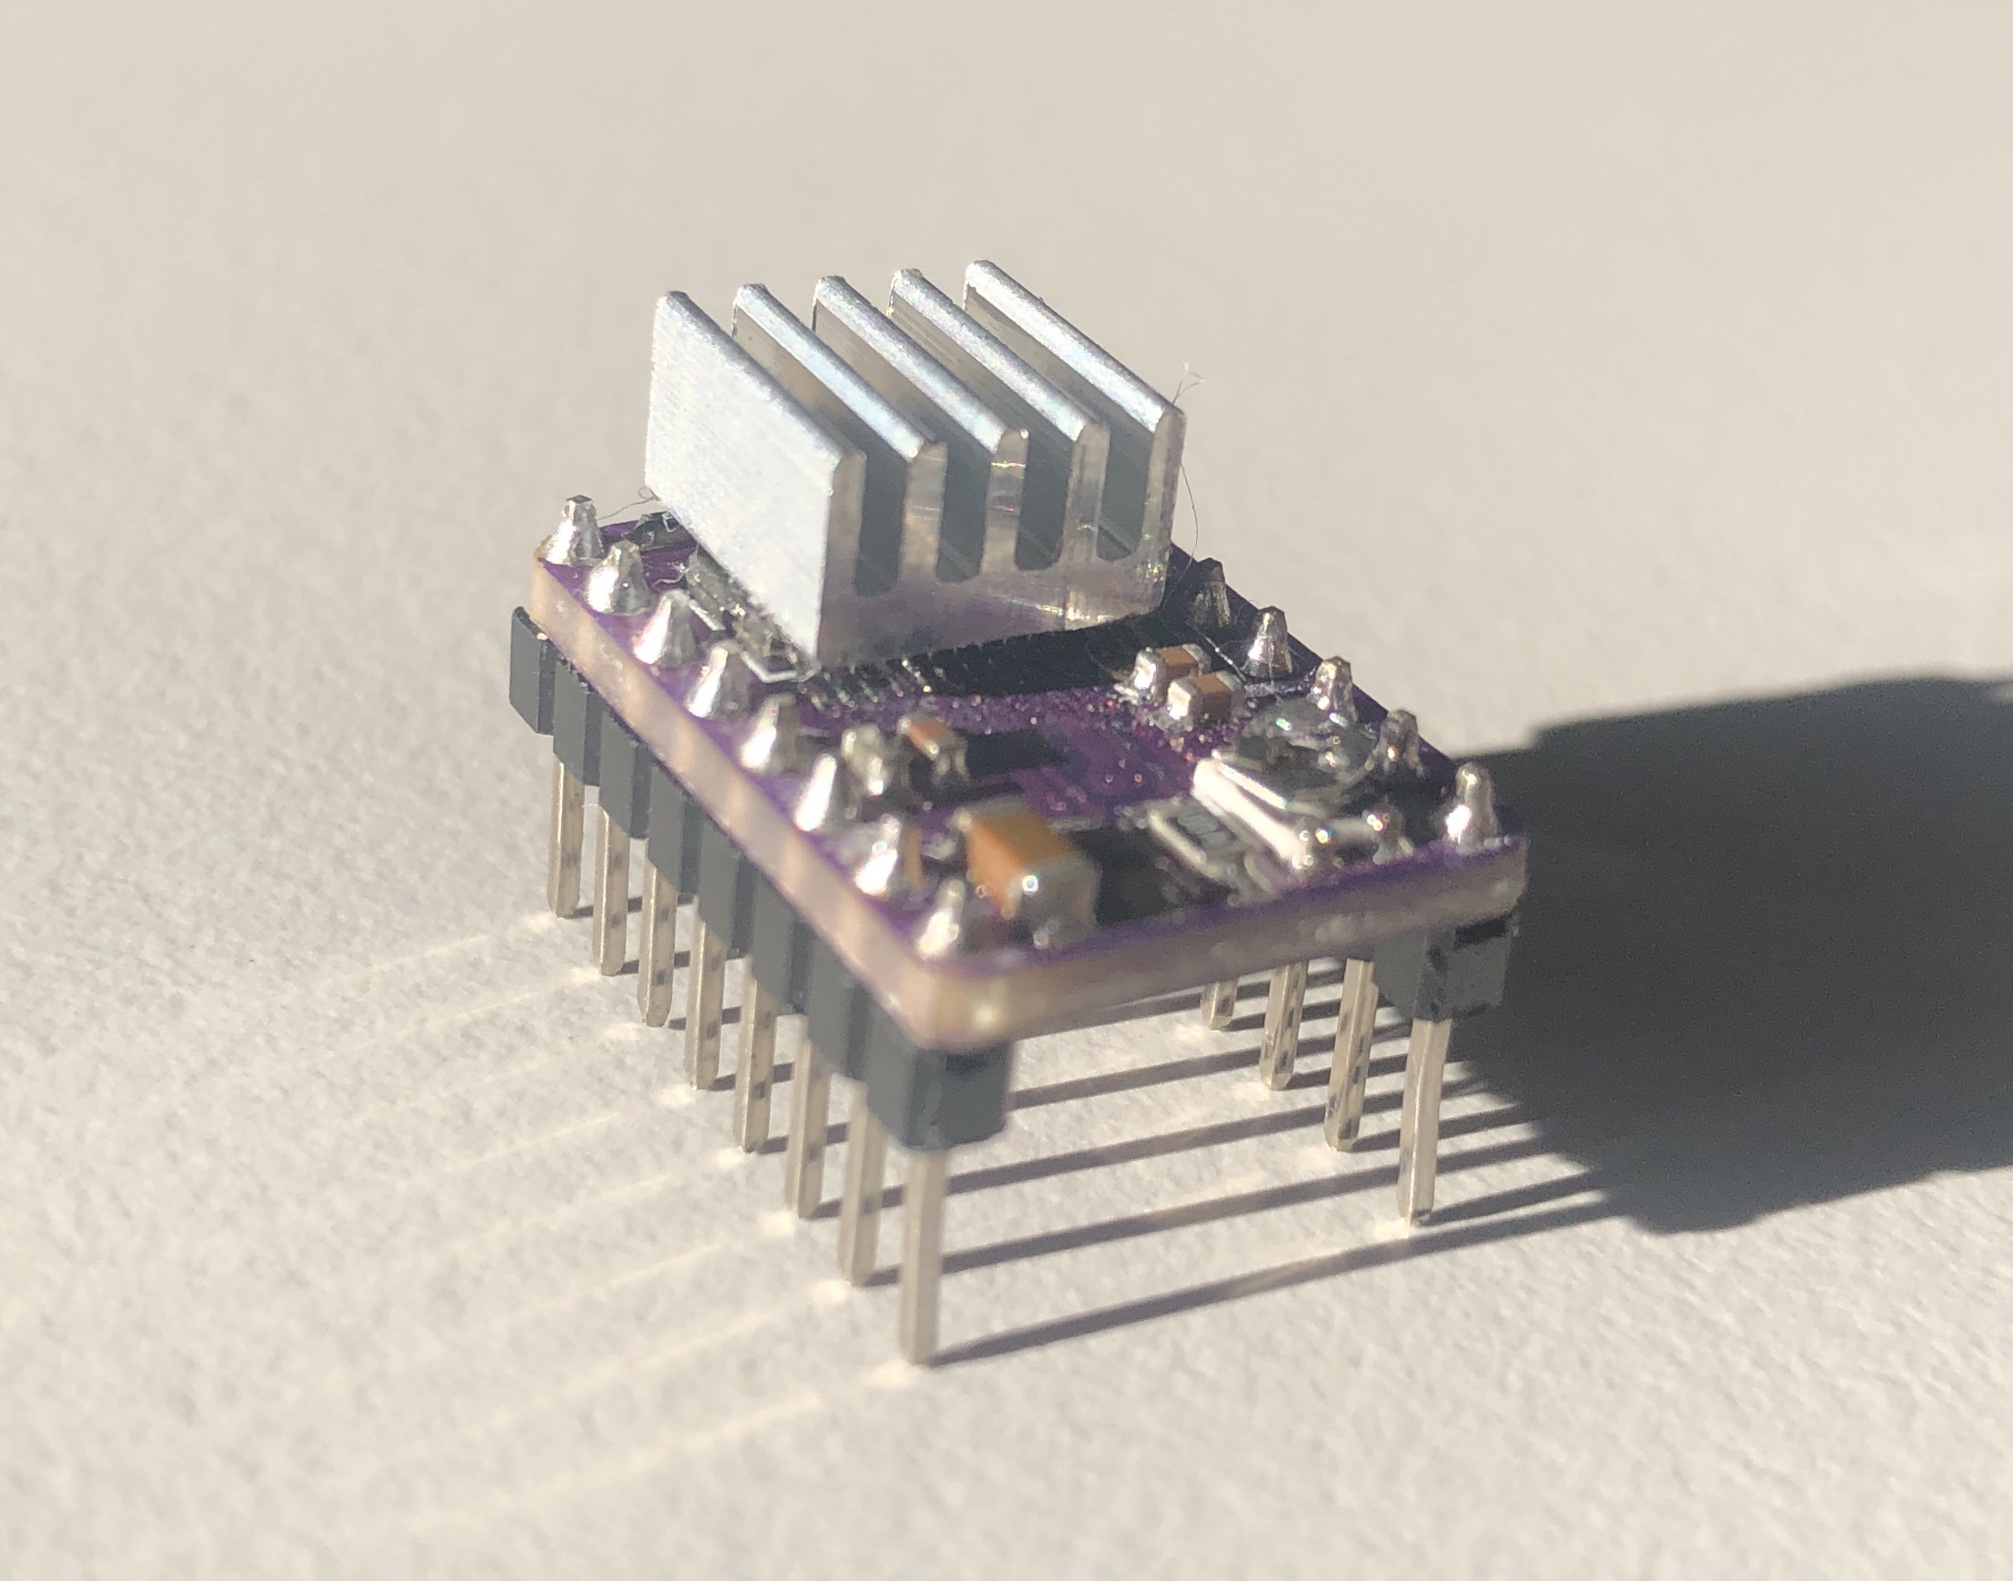
\includegraphics[scale=0.08]{fig/elektro/StepperDriver.jpg}
    \captionof{figure}{Bild des Treibers}
\end{minipage}

\subsubsection{Beschaltung}

\begin{figure}[ht]
    \centering
    \begin{circuitikz}{european, scale = 1}
        \draw [line width=1.5pt](5,0) to (8,0) to (8,4.5) to (5,4.5) to (5,0);

        \draw (5,0.5) to [short,-o](4,0.5)node[anchor=east]{DIR};
        \draw (5,1) to [short,-o](4,1)node[anchor=east]{STEP};
        \draw (4.95,1.5) to [short,o-o](4,1.5)node[anchor=east]{/SLEEP};
        \draw (4.95,2) to [short,o-o](4,2)node[anchor=east]{/RESET};
        \draw (5,2.5) to [short,-o](4,2.5)node[anchor=east]{M2};
        \draw (5,3) to [short,-o](4,3)node[anchor=east]{M1};
        \draw (5,3.5) to [short,-o](4,3.5)node[anchor=east]{M0};
        \draw (4.95,4) to [short,o-o](4,4)node[anchor=east]{/EN};

        \draw (5,0.5) to (5,0.5)node[anchor=west]{DIR};
        \draw (5,1) to (5,1)node[anchor=west]{STEP};
        \draw (5,1.5) to (5,1.5)node[anchor=west]{/SLEEP};
        \draw (5,2) to (5,2)node[anchor=west]{/RESET};
        \draw (5,2.5) to (5,2.5)node[anchor=west]{M2};
        \draw (5,3) to (5,3)node[anchor=west]{M1};
        \draw (5,3.5) to (5,3.5)node[anchor=west]{M0};
        \draw (5,4) to (5,4)node[anchor=west]{/EN};

        \draw (8,0.5) to (8,0.5)node[anchor=east]{GND};
        \draw (8,1) to (8,1)node[anchor=east]{/FLT};
        \draw (8,1.5) to (8,1.5)node[anchor=east]{A2};
        \draw (8,2) to (8,2)node[anchor=east]{A1};
        \draw (8,2.5) to (8,2.5)node[anchor=east]{B1};
        \draw (8,3) to (8,3)node[anchor=east]{B2};
        \draw (8,3.5) to (8,3.5)node[anchor=east]{GND};
        \draw (8,4) to (8,4)node[anchor=east]{VMOT};

        \draw (8,0.5) to (9, 0.5) to (9,0)node[rground]{};
        \draw (8.05,1) to [short,o-](8.5, 1);
        \draw [line width=1pt](8.4,1.1) to (8.6,0.9);
        \draw [line width=1pt](8.4,0.9) to (8.6,1.1);
        \draw (8,1.5) to [short,-o](9, 1.5);
        \draw (8,2) to [short,-o](9, 2);
        \draw (8,2.5) to [short,-o](9, 2.5);
        \draw (8,3) to [short,-o](9, 3);
        \draw (8,3.5) to (10.5, 3.5) to (11.5,3.5);
        \draw (11,3.5) to [short,*-](11,3.5)node[rground]{};
        \draw (8,4) to (10.5, 4) to (10.5,5) to (11.5,5) to [eC, l=$C1$](11.5,3.5);
        \draw (11,5) to [short,*-](11,5)node[vcc]{12V};
        \draw (9,2.75) to (9,2.75)node[anchor=west]{Coil 1};
        \draw (9,1.75) to (9,1.75)node[anchor=west]{Coil 2};
        \draw (5,5.1) to (5,5.1)node[anchor=north]{DRV8825};
    \end{circuitikz}
    \caption{Gewöhnliche externe Beschaltung des Treibers}
    \label{fig:Treiber}
\end{figure}

\newpage

\subsubsection{Beschaltungs- und Anschlussfunktionen}

\begin{figure}[htb]
    \centering
    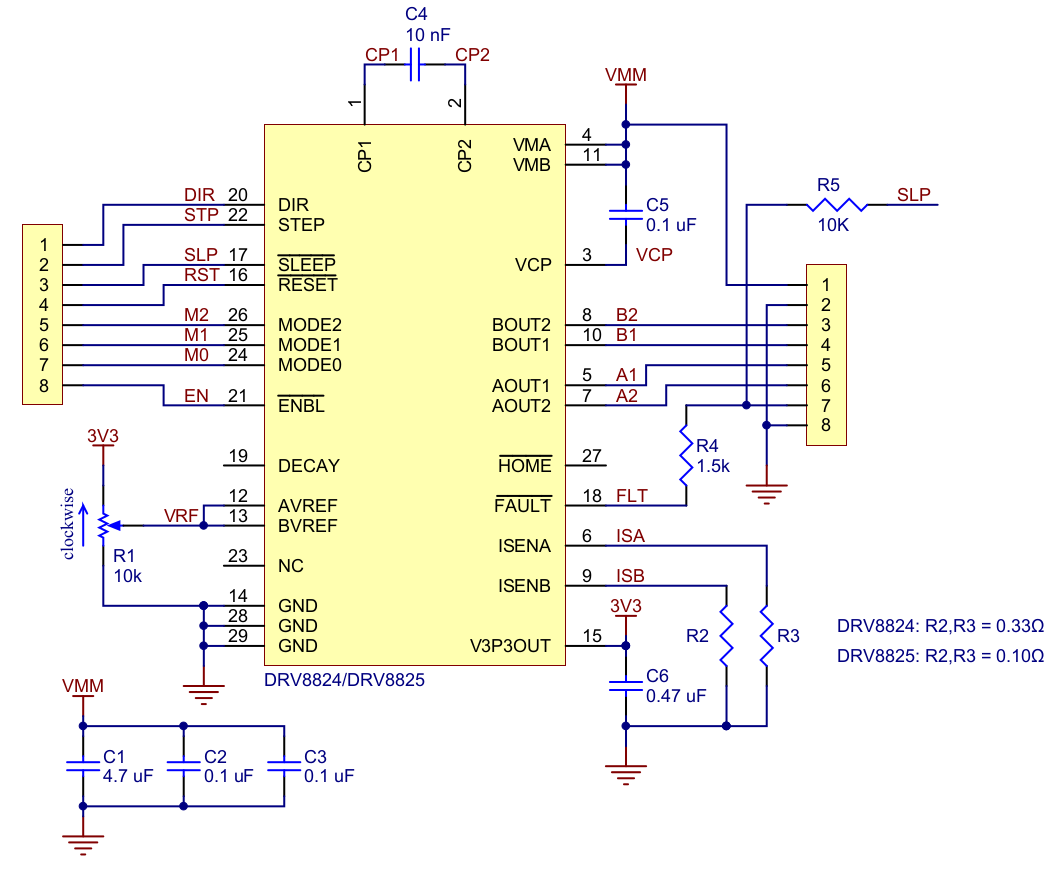
\includegraphics[scale=0.25]{fig/elektro/drv8825.png}
    \caption{Beschaltung des DRV8825-Treiberchips}
    \label{fig:Treiberchip}
\end{figure}

\footfullcite{DRV8825-Datasheet}Der DRV8825 besitzt 16 Anschlüsse.
Drei dieser Anschlüsse fungieren zur Spannungsversorgung: VMOT und die beiden GND Anschlüsse. \\

An dem Anschluss VMOT werden in unserem Fall 12V angelegt.
Diese Trägerplatine benutzt niedrige-\acs{ESR} Keramikkondensatoren, welche sie anfällig für zerstörerische LC-Spannungsspitzen machen.
Insbesondere, wenn längere Stromkabel verwendet werden.
Unter den falschen Bedingungen können diese Spannungsspitzen die maximale Spannung von 45 V für den DRV8825-Treiber überschreiten und der Platine dauerhafte Schäden beisetzen.
Bei der Beschaltung der Spannungsversorgung des DRV8825 wird vom Hersteller der Gebrauch eines Elektrolytkondensators von mindestens 47µF in der Nähe des Treibers empfohlen, um diese Gefahr zu negieren.
Aufgrund dessen entschieden wir uns dazu, einen derartigen Kondensator zu implementieren.\\

An die Anschlüsse B2, B1, A1 und A2 werden die Windungen des Schrittmotors mit dem Treiber verbunden.
Hierbei ist auf die richtige Zusammengehörigkeit zu achten:
Die Anschlüsse B1 und B2 sind mit der einen Windung des Motors zu verbinden, A1 und A2 mit der anderen. \\

Der /FLT (Fault)  Anschluss kann als Statusüberwachung genutzt werden.
Er liefert ein LOW-Pegel Signal, falls der Treiber eine zu hohe Temperatur oder einen zu hohen Strom detektiert.
Im Grundzustand besitzt der Pin durch einen 10k$\Omega$ Pull-Up-Widerstand ein Potential von 3.3V.
Er fungiert als Open-Drain-Output.

\newpage
Die Treiberplatine verfügt 8 Logikanschlüsse, welche auf der linken Seite des Treibers in \autoref{fig:Treiber} zu finden sind: \\

Der /EN Anschluss sorgt bei einem eingehenden HIGH-Signal dafür, dass die H-Brücken deaktiviert und das STEP Eingangssignal nicht berücksichtigt wird.
Bei einem eingehenden LOW-Signal ist der Treiber aktiviert.
Somit sind die H-Brücken aktiviert und steigende Flanken am STEP Anschluss werden eingelesen und verarbeitet.
Durch einen internen Pull-down Widerstand ist dieser Pin auch im nicht beschaltenen Zustand auf LOW. \\

Über die Anschlüsse M0, M1 und M2 ist es möglich, die gewünschte Mikroschrittauflösung zu wählen.
Lässt man diese unbeschalten, sorgen interne Pull-down Widerstände dafür, dass diese auf LOW gezogen werden.
Eine Übersicht der Mikroschrittauflösungen befindet sich im Kapitel 2.3.6.4 . \\

Der Anschluss /RESET sorgt bei einem LOW-Signal für einen Reset der internen Logik und deaktiviert die H-Brücken Treiberbausteine. \\

Ein Anlegen eines HIGH-Signals am invertierten Eingang /SLEEP versetzt den Treiber in einen stromsparenden Schlafzustand. \\

Um den Treiber in voller Funktion verwenden zu können, müssen die Anschlüsse /RESET und /SLEEP mit einem HIGH-Signal versorgt werden. \\

Der STEP Anschluss des DRV8825 liest ein Rechtecksignal ein.
Bei jeder steigenden Flanke rückt der Indexer um einen Schritt weiter. \\

Die Drehrichtung des Motors wird über den DIR Anschluss gesteuert.
Ein HIGH-Pegel am Anschluss bewirkt eine Drehrichtung des Motors im Uhrzeigersinn, ein LOW-Pegel sorgt für eine Drehrichtung gegen den Uhrzeigersinn.

\newpage
\subsubsection{Schrittauflösung}
\footfullcite{DRV8825-Datasheet}In der folgend zu sehenden Tabelle sind die alle Pegelkombinationen der Modus-Anschlüsse dargestellt.
Um die jeweilig gewünschte Mikroschrittauflösung zu erreichen, müssen die Anschlüsse M2, M1 und M0 mit dem entsprechenden Spannungspegel versorgt werden.

\begin{table}[h]
    \centering
    \begin{tabular}{|c|c|c|c|}
        \hline
        \textbf{M2} & \textbf{M1} & \textbf{M0} & \textbf{Schrittauflösung}    \\ \hline
        0 & 0 & 0 & Vollschritt                  \\ \hline
        0 & 0 & 1 & ½ Schritt                    \\ \hline
        0 & 1 & 0 & ¼ Schritt                    \\ \hline
        0 & 1 & 1 & 8 Mikroschritte pro Schritt  \\ \hline
        1 & 0 & 0 & 16 Mikroschritte pro Schritt \\ \hline
        1 & 0 & 1 & 32 Mikroschritte pro Schritt \\ \hline
        1 & 1 & 0 & 32 Mikroschritte pro Schritt \\ \hline
        1 & 1 & 1 & 32 Mikroschritte pro Schritt \\ \hline
    \end{tabular}
    \caption{Festlegen der Schrittauflösung}
\end{table}

\subsubsection{Stromlimitierung}
\footnotemark[14]Um den durch die Motorwindungen fließenden Strom zu limitieren, kann dem Datenblatt des DRV8825 folgende Formel entnommen werden:

\begin{equation}
    I_{max} = \frac{V_{ref}} {5 \cdot R_{sense}}
\end{equation}

Der von uns ausgewählte Schrittmotor 17HS19-2004S1 braucht laut dessen Datenblatt einen Strom von 2A .
Durch einige Tests und Messungen fanden wir jedoch heraus, dass 1.6A bei gewöhnlichem Betrieb mehr als genug sind.
Um nun die Stromlimitierung auf 1.6A einzustellen, muss die Referenzspannung adaptiert werden.

\begin{equation*}
    V_{ref} = I_{max} \cdot 5 \cdot R_{sense}
\end{equation*}

Der R\textsubscript{sense} kann der \autoref{fig:Treiberchip} entnommen werden.
Beim DRV8825 beträgt der Wert 0.1 Ohm.

\begin{align*}
    V_{ref} &= 1.6A \cdot 5 \cdot 0.1\Omega \\
    V_{ref} &= 0.8V
\end{align*}
Die Berechnung ergibt, dass für einen Strom von 1.6A, eine Referenzspannung von 0.8V eingestellt werden muss.
Diese Spannung kann mithilfe eines Potentiometers, welches sich auf dem Treibermodul befindet (siehe \autoref{fig:Treiberchip}), eingestellt werden.

\newpage
\subsubsection{Kühlkörperberechnung}
Um die Notwendigkeit eines Kühlkörpers zu berechnen, werden folgende Formeln benötigt:

\begin{equation}
    P_D = \frac{(T_{jmax} - T_{ha} - Sicherheit)}{R_{thja}}
\end{equation}

\begin{equation}
    P_V = R_{DSon} \cdot I_{max}^2
\end{equation}

Sollte die Verlustleistung P\textsubscript{V} größer als P\textsubscript{D} sein, ist ein Kühlkörper notwendig. \\

\textbf{Datenblattwerte}\\
• T\textsubscript{jmax} = 150°C (Maximale Sperrschicht-Temperatur)\\
• T\textsubscript{a} = 25°C (Umgebungstemperatur)\\
• R\textsubscript{thjc} = 15.9°C/W (Wärmewiderstand zwischen Sperrschicht und Gehäuse)\\
• R\textsubscript{thja} = 31.6°C/W (Wärmewiderstand zwischen Sperrschicht und Umgebung)\\
• R\textsubscript{thiso} = 0.1°C/W (Wärmewiderstand der Montagefläche)\\
• R\textsubscript{DSon} = 0.32 Ohm (Drain-Source On-State Resistance)

\begin{align*}
    P_V &= R_{DSon} \cdot I_{max}^2 \\
    P_V &= 0,32\Omega \cdot 1.6A^2 \\
    P_V &= 0.8192W
\end{align*}

\begin{align*}
    P_D &= \frac{(T_{jmax} - T_{a} - Sicherheit)}{R_{thja}} \\
    P_D &= \frac{150^{\circ}C - 25^{\circ}C - 25^{\circ}C}{31.6\frac{{}^{\circ}C}{W}} \\
    P_D &= 3.1646W
\end{align*}

Durch die Berechnung lässt sich beweisen, dass kein Kühlkörper notwendig ist.
Um jedoch Gewissheit zu erlangen, ist die maximal erreichte Sperrschichttemperatur bei sommerlichen Tempraturen zu berechnen.

\begin{align*}
    T_{j} &= (T_{a}+Sicherheit) + {R_{thja}} \cdot P_{v}) \\
    T_{j} &= (25^{\circ}C + 25^{\circ}C) + 31.6\frac{{}^{\circ}C}{W} \cdot 0.8192W \\
    T_{j} &= 75.8867^{\circ}C
\end{align*}
\newpage
Der Umstand einer Umgebungstemperatur von 50°C führt somit bewiesenerweise dennoch zu einem zulässigem Betrieb.
Jedoch wird vom Hersteller ausdrücklich empfohlen einen Kühlkörper zu verwenden, sobald ein Strom größer als 1A getrieben wird, wodurch schlussendlich ein Kühlkörper auf dem Treiber platziert wurde.

Für die Berechnung des Kühlkörperwärmewiderstandes R\textsubscript{thK} wird von folgender Formel Gebrauch gemacht:

\begin{align}
    R_{thK} &= \frac{T_{jmax} - T_{ha} - Sicherheit}{P_V} - (R_{thiso} + R_{thjc}) \\
    R_{thK} &= \frac{150^{\circ}C - 25^{\circ}C - 25^{\circ}C}{0,8192W} - (0.1\frac{{}^{\circ}C}{W} + 15.9\frac{{}^{\circ}C}{W}) \notag \\
    R_{thK} &= 106.07\frac{{}^{\circ}C}{W}  \notag
\end{align}

Die Berechnung zeigt, dass die Verwendung eines Kühlkörpers nicht unvorteilhaft wäre, weshalb wir den mitgelieferten Kühlkörper auch verwenden.
Zu diesem sind keinerlei Werte bekannt, jedoch konnten wir durch einige Tests seine geeignete Funktionalität unter Beweis stellen.

\subsection{Erfassung der Motorposition}

Zu Beginn wird der Schrittmotor in eine Richtung angesteuert, bis er seinen Referenzpunkt erreicht, welcher als Mikroschalter implementiert ist.
Der vom Mikrocontroller auf "HIGH" gesetzte Ausgang wird bei einer Betätigung des Mikroschalters gegen Masse geschalten.
Der Zustand dieses Ausgangs wird über das zugehörige PIN-Register vom Mikrocontroller eingelesen und folgend mit Software über eine Led visuell dargestellt.
So können ausgehend vom Referenzpunkt Schrittzahlen zu gewünschten Positionen aufgetragen werden.

\begin{figure}[hpt]
    \centering
    \begin{circuitikz}[european, scale = 0.7]

        \draw [line width=1.5pt](-4,5) to (-1,5) to (-1,10);
        \draw (-2,8.5)node[vcc]{Vcc};
        \draw (-2,8.5) to [R,l_=$R1$](-2,6) to (-1,6);
        \draw (-1,6) to (0,6) to (0,5) to [short, -o](1,5);
        \draw (1,4) to [short, o-](0,4) to (0,3);
        \draw (1,4.5) to (1,4.5)node[anchor=west]{Mikroschalter};
        \draw (-3.5,5)node[anchor=south]{µC};
        \draw (0,3) to (0,2) node[rground]{};
    \end{circuitikz}
    \caption{Erfassung der Schrittmotorposition}
\end{figure}

\newpage
\subsection{Kapazitive Sensoren}

Die von uns ausgewählten Sensoren LJC18A3-BZ/BX besitzen jeweils drei Anschlüsse:
einen blauen, welcher mit Ground zu verbinden ist, einen braunen, der mit einer Versorgungsspannung von 6V bis 36V zu verbinden ist sowie einen schwarzen, über den das Signal vermittelt wird. \\

\textbf{Eigenschaften:}
\begin{itemize}
    \item Schaltabstand 1 bis 10mm, einstellbar durch Stellschraube
    \item Betriebsspannung 6V-36V
    \item Maximale Last 300mA
    \item Ausgang realisiert durch einen NPN-Schließer
\end{itemize}

In unserem Fall werden alle kapazitiven Sensoren mit 12V versorgt.
Der Signalausgang des Sensors liefert im Grundzustand ein HIGH-Signal.
Sobald ein Objekt in das Messumfeld des Sensors gelangt, liefert dieser ein Signal von 0.62V, welches als LOW-Signal gilt.
Um den HIGH-Pegel für den Mikrocontroller lesbar zu gestalten, ist ein Spannungsteiler am Signalausgang des Sensors zu dimensionieren.

\begin{figure}[ht]
    \centering
    \begin{circuitikz}[european, scale = 1.2]
        \draw (0,0) node[anchor=east] {-} to [short, o-*] (4,0);
        \draw (1,3) to [short, -o](0,3)node[anchor=east]{+};
        \draw (4,3) to [R, l_=$R2$, v^=$U2$, *-] (4,0);
        \draw (1,3) to[R, l=$R1$, v_>=$U1$](4,3) to [short, -o](6,3)node[anchor=west]{+};
        \draw (4,0) to [short, *-o](6,0)node[anchor=west]{-};
        \draw (4,0) to (4,0) node[rground]{};
        \draw (0,2.8) -- node[left] {$U_\mathrm{Sensor}$}node[sloped,currarrow,pos=1] {}(0,0.2);
        \draw (6,2.8) -- node[right] {$U_\mathrm{Mikrocontroller}$}node[sloped,currarrow,pos=1] {}(6,0.2);
    \end{circuitikz}
    \caption{Aufbau einer Spannungsteilers}
\end{figure}

Durch verschiedene Tests gelangten wir zur Erkenntnis, dass sich der Spannungspegel des Sensorausgangssignals je nach Spannungsteiler ändert.
Durch sukzessive Annäherung an die gewünschten 3.3V Ausgangsspannung wurden folgende Werte als günstige Lösung gewählt:

\begin{equation*}
    R_1 = 5.6k\Omega, R_2 = 4.7k\Omega
\end{equation*}

Durch diese Werte ergibt sich bei einer HIGH Signalausgangsspannung von 6.92V eine Spannung am Ausgang des Spannungsteilers von 3.31V .
Bei einem LOW-Pegel ist am Ausgang des Spannungsteilers eine Spannung von 0.29V zu messen.
Da die Schaltschwelle der I/O Pins des ATmega324PA bei LOW-Pegeln maximal 0.99V und die bei HIGH-Pegeln mindestens 1.98V beträgt, wurden diese gemessenen Werte als zulässige bewertet.

\newpage
\subsection{Ansteuerung der Hubmagneten}

Als Ansteuerung der beiden Hubmagneten wird jeweils die unten zu sehende Schaltung angewandt.
Auf einen Bipolartransistor wurde nicht zurückgegriffen, da dieser nicht in der Lage dazu wäre Ströme von 350mA ohne Überhitzung zu schalten.

\subsubsection{Funktion}

Sobald die Gate-Source-Schwellenspannung des MOSFETs mithilfe eines 3.3V Signals ausgehend vom Mikrocontroller überschritten wird, schaltet der N-Kanal MOSFET durch.
Dieser ermöglich das Fließen des Drainstromes durch den Hubmagneten zum Massepotential.
Um den fließenden Gate-Strom zu verringern, wurde der Widerstand R1 implementiert.
Der Widerstand R2 hingegen hat den Nutzen, parasitäre Kapazitäten des MOSFETs zu entladen.
Um keinen Spannungsteiler und somit einen Spannungsabfall von rund 5 Prozent der Eingangsspannung zu verursachen, ist der Widerstand vor den Widerstand R1 zu schalten.
Da es sich bei den Hubmagneten um eine induktive Last handelt, ist es erforderlich parallel eine sogenannte Fleilaufdiode zu schalten.
Diese hat die Aufgabe, den MOSFET vor einem selbsterzeugten, rückfließenden Strom des Hubmagneten zu schützen.


\begin{figure}[hpt]
    \centering
    \begin{circuitikz}[european, scale = 1]
        \draw (5,8)node[vcc]{+12V};
        \draw (5,8) to (5,6.5) to [short, -o](6,6.5);
        \draw (6,5.5) to [short, o-](5,5.5) to (5,3.5);
        \draw (5,5) to [short, *-](4,5) to [/tikz/circuitikz/bipoles/length=1cm, D, l=$D1$](4,7) to [short, -*](5,7);
        \draw (4,5) to (4,7);
        \draw (6,6) to (6,6)node[anchor=west]{Hubmagnet};
        \draw (5,3) to (5,0);
        \draw (4.1,3) to (3.5,3) to [R, l_= $R1$](1.5,3) to [short, -o](-0.5,3);
        \draw (2,2.5)node[anchor=west]{560};
        \draw (1,3) to [short,*-](1,3) to [R, l_=$R2$](1,0) to [short,-*](5,0) to (5,-0.5);
        \draw (1.1,1.5)node[anchor=west]{10k};
        \draw (5,3)node[nfet, solderdot, bodydiode](nfet){};
        \draw (nfet.G) node[above]{G};
        \draw (nfet.D) node[left]{D};
        \draw (nfet.S) node[left]{S};
        \draw (-0.5,3) to (-0.5,3)node[anchor=east]{SIG};
        \draw (5,-0.5) to (5,-0.5) node[rground]{};
    \end{circuitikz}
    \caption{Ansteuerung der Hubmagneten}
\end{figure}

\newpage

\subsection{Ansteuerung der Pumpe und des Ventils}

Um sowohl die Pumpe als auch das Ventil ansteuern zu können, wurde jeweils von der Schaltungsstruktur jener Schaltung, welche die Hubmagneten ansteuert, Gebrauch gemacht.

\subsubsection{Funktion}

Mithilfe eines 3.3V Steuersignals, ausgehend vom ATmega324PA, wird die Gate-Source-Schwellspannung des N-Kanal-MOSFET überschritten.
Somit schaltet der MOSFET die am Drain anliegende Leitung auf Masse und Strom fließt vom Drain zur Source.
Um den fließenden Gate-Strom des Steuersignals zu begrenzen, wurde auf einen Widerstand, hier R1, zurückgegriffen.
Um jene am MOSFET anfallende, parasitäre Kapazitäten zu negieren, wurde der Widerstand R2 vorgesehen.
Die Pumpe sowie das Ventil stellen eine induktive Last dar, welche den Nutzen einer Freilaufdiode erfordern, da diese ansonsten den MOSFET durch ihren selbst induzierten Strom gefährden könnten.

\begin{figure}[hpt]
    \centering
    \begin{circuitikz}[european, scale = 0.8]
        % Pumpe
        \draw (5,8)node[vcc]{+5V};
        \draw (5,8) to (5,6.5) to [short, -o](6,6.5);
        \draw (6,5.5) to [short, o-](5,5.5) to (5,3.5);
        \draw (5,5) to [short, *-](4,5) to [/tikz/circuitikz/bipoles/length=1cm, D, l=$D1$](4,7) to [short, -*](5,7);
        \draw (4,5) to (4,7);
        \draw (6,6) to (6,6)node[anchor=west]{Pumpe};
        \draw (5,3) to (5,0);
        \draw (4.1,3) to (3.5,3) to [R, l_= $R1$](1.5,3) to [short, -o](-0.5,3);
        \draw (2,2.4)node[anchor=west]{560};
        \draw (1,3) to [short,*-](1,3) to [R, l_=$R2$](1,0) to [short,-*](5,0) to (5,-0.5);
        \draw (1.1,1.5)node[anchor=west]{10k};
        \draw (5,3)node[nfet, solderdot, bodydiode](nfet){};
        \draw (nfet.G) node[above]{G};
        \draw (nfet.D) node[left]{D};
        \draw (nfet.S) node[left]{S};
        \draw (-0.5,3) to (-0.5,3)node[anchor=east]{SIG};
        \draw (5,-0.5) to (5,-0.5) node[rground]{};

        % Ventil
        \draw (15,8)node[vcc]{+5V};
        \draw (15,8) to (15,6.5) to [short, -o](16,6.5);
        \draw (16,5.5) to [short, o-](15,5.5) to (15,3.5);
        \draw (15,5) to [short, *-](14,5) to [/tikz/circuitikz/bipoles/length=1cm, D, l=$D2$](14,7) to [short, -*](15,7);
        \draw (14,5) to (14,7);
        \draw (16,6) to (16,6)node[anchor=west]{Ventil};
        \draw (15,3) to (15,0);
        \draw (14.1,3) to (13.5,3) to [R, l_= $R3$](11.5,3) to [short, -o](9.5,3);
        \draw (12,2.4)node[anchor=west]{560};
        \draw (11,3) to [short,*-](11,3) to [R, l_=$R4$](11,0) to [short,-*](15,0) to (15,-0.5);
        \draw (11.1,1.5)node[anchor=west]{10k};
        \draw (15,3)node[nfet, solderdot, bodydiode](nfet1){};
        \draw (nfet1.G) node[above]{G};
        \draw (nfet1.D) node[left]{D};
        \draw (nfet1.S) node[left]{S};
        \draw (9.5,3) to (9.5,3)node[anchor=east]{SIG};
        \draw (15,-0.5) to (15,-0.5) node[rground]{};
    \end{circuitikz}
    \caption{Ansteuerung der Pumpe und des Ventils}
\end{figure}

\newpage

\subsection{Mini-USB Schnittstelle}

Um Debugging effektiv betreiben zu könnnen, ist eine Verbindung von Mini-USB zu UART implementiert worden.
So können Vorgänge leicht über einen Computer via Kabel überwacht werden oder etwa ein neues Programm herübergespielt werden.

Als USB-zu-UART-Converter wählten wir den CH340G aus, für dessen Wahl seine geringen Kosten, die kleine Gehäusebauform sowie ein Treiber im Linux-Kernel sprach.\\
\footfullcite{Datasheet-CH340G}Dieser Treiberbaustein ist wie folgt zu beschalten:

\begin{figure}[ht]
    \centering
    \begin{circuitikz}[european, scale = 1.15]

        %Mini-USB
        \draw [line width=1.5pt](-1,1) to (-1,3.5) to (1,3.5) to (1,1) to (-1,1);
        \draw (1,3) to (1.5,3) to [/tikz/circuitikz/bipoles/length=1cm, sD, l=$D1$](1.5,6) to (1.5,3);
        \draw (1,2.5) to (1.5,2.5);
        \draw (1,2) to (1.5,2);
        \draw (1,1.5) to (1.5,1.5);
        \draw (1,1.5) to (1,1.5)node[anchor=east]{ID};
        \draw (1,2) to (1,2)node[anchor=east]{D-};
        \draw (1,2.5) to (1,2.5)node[anchor=east]{D+};
        \draw (1,3) to (1,3)node[anchor=east]{VBUS};
        \draw (-0.6,1.5) to (-0.6,1.5)node[anchor=north]{SH};
        \draw (0.1,1.5) to (0.1,1.5)node[anchor=north]{GND};

        %Unconnected Pins
        \draw (1.6,1.6) to (1.4,1.4);
        \draw (1.6,1.4) to (1.4,1.6);
        \draw (4.4,3.4) to (4.6,3.6);
        \draw (4.4,3.6) to (4.6,3.4);

        \draw (8.6,0.6) to (8.4,0.4);
        \draw (8.4,0.6) to (8.6,0.4);
        \draw (8.6,1.6) to (8.4,1.4);
        \draw (8.4,1.6) to (8.6,1.4);
        \draw (8.6,2.1) to (8.4,1.9);
        \draw (8.4,2.1) to (8.6,1.9);
        \draw (8.6,2.6) to (8.4,2.4);
        \draw (8.4,2.6) to (8.6,2.4);
        \draw (8.6,3.1) to (8.4,2.9);
        \draw (8.4,3.1) to (8.6,2.9);

        \draw (5,3.5) to (5,3.5)node[anchor=west]{RS232};
        \draw (5, 2) to (1, 2);
        \draw (5,2) to (5,2)node[anchor=west]{UD-};
        \draw (5,2.5) to (1,2.5);
        \draw (5,2.5) to (5,2.5)node[anchor=west]{UD+};
        \draw (6,4.55) to (6,4.55)node[anchor=north]{V3};
        \draw (7,4.55) to (7,4.55)node[anchor=north]{VCC};
        \draw (8,4) to (8,4)node[anchor=east]{TXD};
        \draw (8,3.5) to (8,3.5)node[anchor=east]{RXD};
        \draw (8,3) to (8,3)node[anchor=east]{CTS};
        \draw (8,2.5) to (8,2.5)node[anchor=east]{DSR};
        \draw (8,2) to (8,2)node[anchor=east]{RT};
        \draw (8,1.5) to (8,1.5)node[anchor=east]{DCD};
        \draw (8,1) to (8,1)node[anchor=east]{DTR};
        \draw (8,0.5) to (8,0.5)node[anchor=east]{RTS};

        \draw [line width = 1.2](7.15,0.7) to (7.85,0.7);
        \draw [line width = 1.2](7.15,1.2) to (7.85,1.2);
        \draw [line width = 1.2](7.15,1.7) to (7.85,1.7);
        \draw [line width = 1.2](7.4,2.2) to (7.85,2.2);
        \draw [line width = 1.2](7.15,2.7) to (7.85,2.7);
        \draw [line width = 1.2](7.15,3.2) to (7.85,3.2);


        %USB to UART - Modul
        \draw [line width=1.5pt](5,0) to (8,0) to (8,4.5) to (5,4.5) to (5,0);
        \draw (5, 0.5) to (4.5, 0.5) to (4.5,0) to (4,0) to [C](2.5,0);
        \draw (5, 1) to (4.5, 1) to (4.5, 1.5) to (4,1.5) to [C](2.5,1.5) to (2,1.5) to (2,0) to [short,-*](2,0.75) to (1.5,0.75) to (1.5,0.25)node[rground]{};
        \draw (4,1.5) to [PZ, l_=$Y1$, *-*](4,0);
        \draw (2,0) to (2.5,0);
        \draw (5,0.5) to (5,0.5)node[anchor=west]{XI};
        \draw (5,1) to (5,1)node[anchor=west]{XO};
        \draw (6.5,0.5) to (6.5,0.5)node[anchor=north]{GND};

        \draw (5,3.5) to (4.5,3.5);
        \draw (6,4.5) to (6,7) to (4.5,7) to [C, l_=$C1$](4.5,5.5) to (4.5,5.5) node[rground]{};;
        \draw (7,4.5) to (7,7.5);
        \draw (7,7 )to [short,*-](8.5,7) to [C, l_=$C2$](8.5,5.5)  to (8.5,5.5) node[rground]{};;;

        \draw (8,0.5) to (8.5, 0.5);
        \draw (8,1) to [short, -o](10, 1)node[anchor=west]{DTR-USB};
        \draw [line width = 1.2](10.1,1.2) to (10.8,1.2);
        \draw (8,1.5) to (8.5, 1.5);
        \draw (8,2) to (8.5, 2);
        \draw (8,2.5) to (8.5, 2.5);
        \draw (8,3) to (8.5, 3);
        \draw (8,3.5) to [short, -o](10, 3.5)node[anchor=west]{RxD-USB};
        \draw (9.5,3.5) to [R, l_=$R1$, *-](9.5,6.5) to (9.5,6.5)node[vcc]{+3.3V};
        \draw (8,4) to [short, -o](10, 4)node[anchor=west]{TxD-USB};;


        %Beschriftungen
        \draw (5,5) to (5,5)node[anchor=north]{CH340G};
        \draw (2.8,0) to (2.8,0)node[anchor=north]{C4};
        \draw (2.8,1.5) to (2.8,1.5)node[anchor=north]{C3};
        \draw (-0.25,4) to (-0.25,4)node[anchor=north]{Mini-USB};
        \draw (1.5,6)node[vcc]{+5V};
        \draw (7,7.5)node[vcc]{+3.3V};
        \draw (-0.5,1) to (-0.5,0.5) node[rground]{};
        \draw (6.5,0) to (6.5,-0.5) node[rground]{};
        \draw (0,1) to (0,0.5) to [short, -*](-0.5,0.5);
    \end{circuitikz}
    \caption{Beschaltung des Mini USB Treibers}
\end{figure}

Neben der vorgeschriebenen Beschaltung wurde zusätzlich die Schottkydiode D1 und ein Pull-Up Widerstand am \acs{RXD}-Pin implementiert.
Die Schottkydiode hat die Aufgabe eine Rückspeisung von 5V zum eingesteckten Gerät zu verhindern.
Der Pull-Up Widerstand fungiert als Prävention einer floatenden Leitung.

\newpage

\subsection{Spannungspegelüberwachung}

Grundsätzlich ist zu sagen, dass an den Spannungspegeln von 12V, 5V und 3.3V sowie an anderen signifikanten Stellen der Platine Messpunkte zur erleichterten Fehlersuche und Wartung realisiert wurden.

Zusätzlich wurden, um jegliche Spannungspegel visuell darzustellen, bei manchen Spannungspegeln eine grüne Leuchtdiode als visuelle, schnelle Funktionsüberwachung integriert.

Am 12V Spannungspegel realiserten wir eine Zenerdiode mit einer Zenerspannung von 8.2V .
Diese ist in Serie mit einem Widerstand und einer Diode geschaltet.

Ein Überwachen des 5V Pegels wurde folgend realisiert:
Zwei Dioden wurden seriell mit einem Widerstand und einer Leuchtdiode geschalten.
Die benötigte Spannung, um ein Leuchten der \acs{LED} zu geährleisten, steigt somit auf etwa 4V .

An dem 3.3V Spannungspegel ist ein Widerstand und eine Leuchtiode in Serie geschaltet, welche ab einer Spannung von 2.2V leuchtet.

\begin{figure}[htp]
    \centering
    \begin{circuitikz}[european, scale = 0.8]
        \draw (1,9)node[vcc]{+3.3V};
        \draw (1,5) to [R, l_=$R1$](1,3){};
        \draw (1,3) to [/tikz/circuitikz/bipoles/length=1.1cm, led, l_=$D1$](1,1);
        \draw (1,3) to (1,0) node[rground]{};
        \draw (3,9)node[vcc]{+5V};
        \draw (3,9) to [/tikz/circuitikz/bipoles/length=1.1cm, D, l_=$D2$](3,7){};
        \draw (3,7) to [/tikz/circuitikz/bipoles/length=1.1cm, D, l_=$D3$](3,5){};
        \draw (3,5) to [R, l_=$R2$](3,3){};
        \draw (3,3) to [/tikz/circuitikz/bipoles/length=1.1cm, led, l_=$D4$](3,1);
        \draw (3,3) to (3,0) node[rground]{};
        \draw (5,9)node[vcc]{+12V};
        \draw (5,5) to [/tikz/circuitikz/bipoles/length=1.1cm, zDo, l=$D5$](5,7);
        \draw (5,5) to [R, l_=$R3$](5,3){};
        \draw (5,3) to [/tikz/circuitikz/bipoles/length=1.1cm, led, l_=$D6$](5,1);
        \draw (5,3) to (5,0) node[rground]{};
        \draw (3,5) to (3,9);
        \draw (1,5) to (1,9);
        \draw (5,5) to (5,9);
    \end{circuitikz}
    \caption{Realisierung der Leuchtdioden}
\end{figure}

\newpage

\subsection{Netzteil-Dimensionierung}

Zur Netzteil-Dimensionierung wurden die maximal möglichen Stromwerte der einzelnen Peripheriebausteine herangezogen.

\begin{table}[h]
    \centering
    \begin{tabular}{|c|c|c|c|}
        \hline
        \textbf{Komponente} & \textbf{maximaler Strom} & \textbf{gemessener Strom im durchschnittlichen Betrieb} \\ \hline
        Hubmagnete & je 350mA & je 323mA \\ \hline
        Schrittmotor & 2000mA & 1600mA \\ \hline
        Sensoren & je 5mA & je 4.3mA \\ \hline
        Pumpe & 280mA & 190mA (ohne Last), 250mA (mit Last) \\ \hline
        Ventil & 260mA & 250mA \\ \hline
        Raspberry Pi 3B+ inkl.\acs{LCD} & 850mA & Idle 600mA, bei intensiver Benutzung 750mA \\ \hline
        ATmega324PA & 60mA & - \\ \hline
        \textbf{Summe} & \textbf{4165mA} & - \\ \hline
    \end{tabular}
    \caption{Überschlagsmäßige Dimensionierung des Netzteils}
\end{table}

Hinzuzufügen ist jedoch, dass in keinem Fall alle Geräte gleichzeitig betrieben werden, sodass der durchschnittliche Dauerstrom weitaus niedriger ausfällt.
Als Netzteil wählten wir ein Schaltnetzteil mit Kaltgerätestecker aus, welches die Aufgabe erfüllt eine Wechselspannung von 230V in eine Gleichspannung von 12V umzuwandeln.
Zudem genügt es unserer Anforderung, einen Strom von 5A bereitstellen zu können.

\begin{figure}
    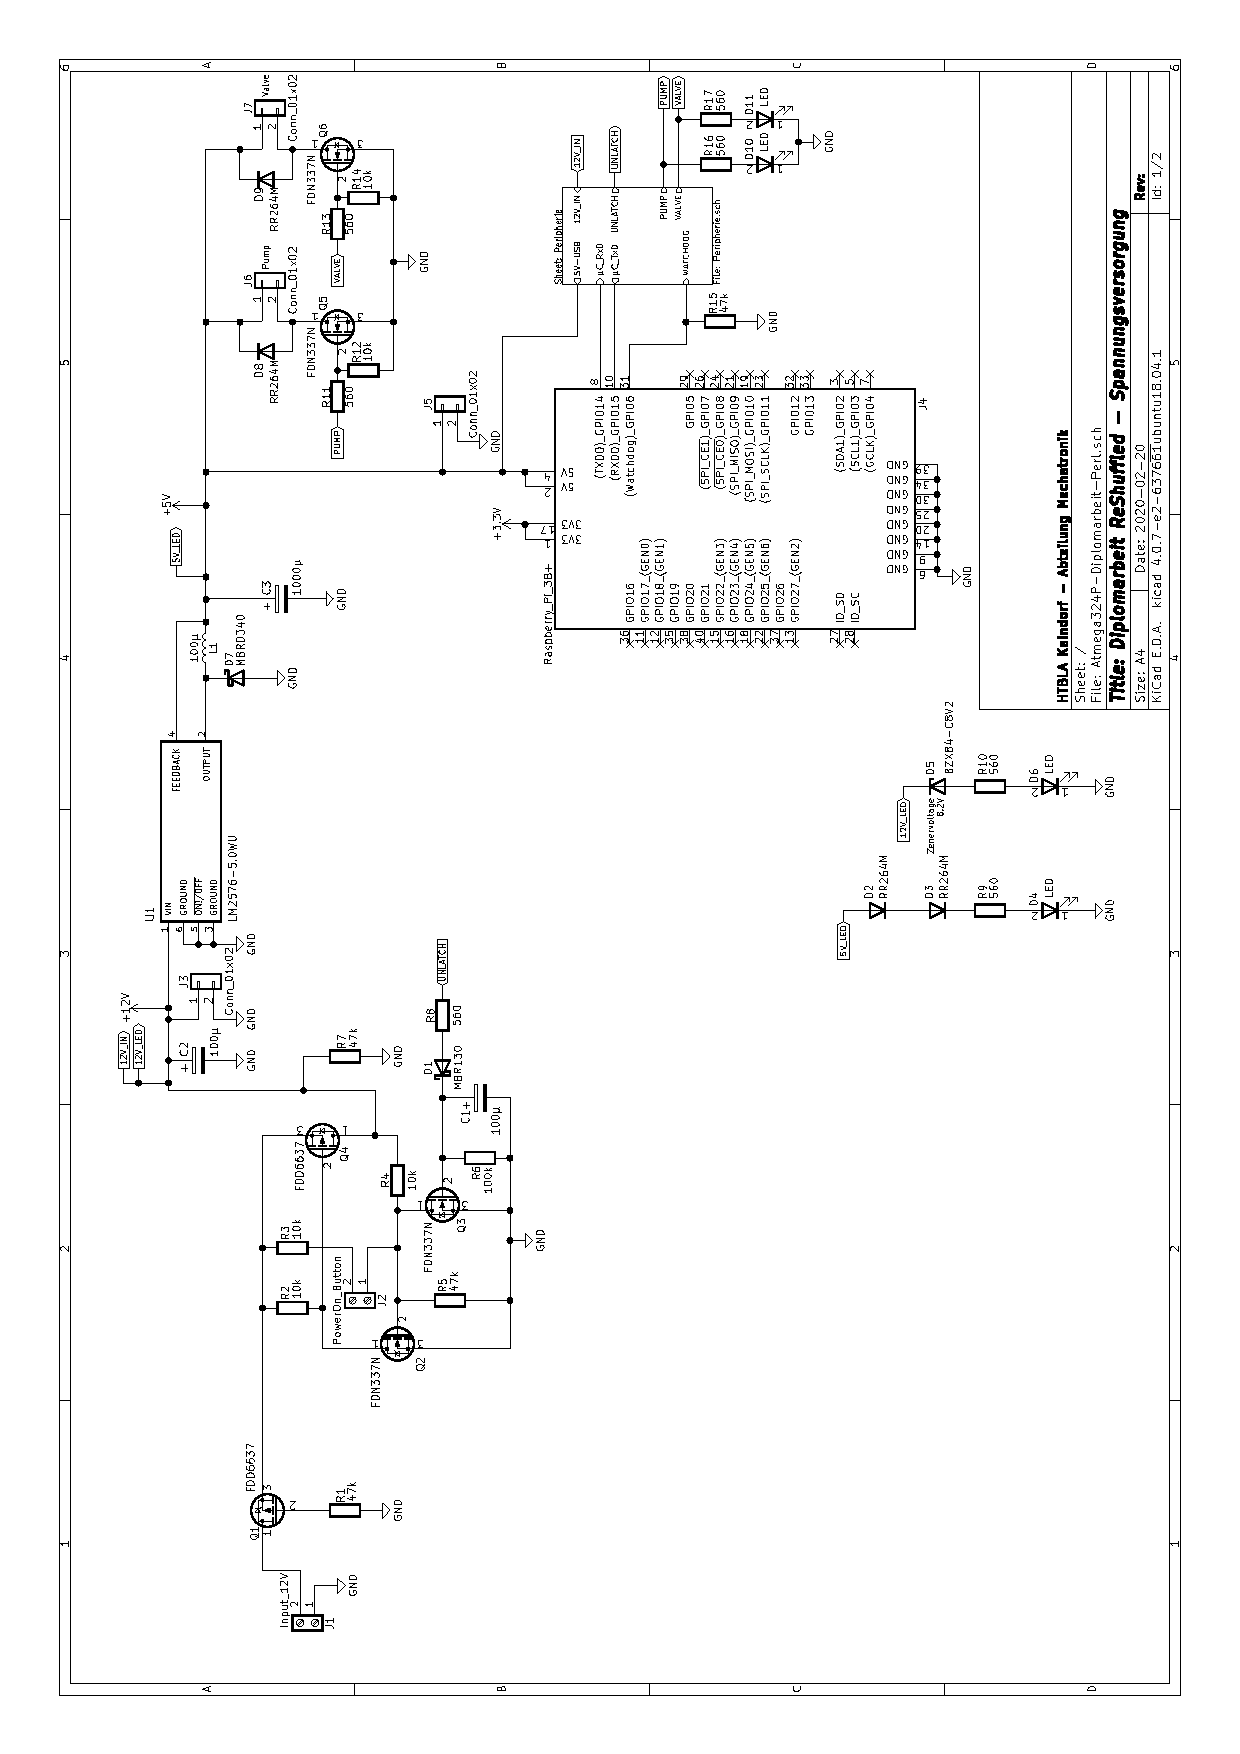
\includegraphics[scale=0.85,page=1]{fig/elektro/Schaltplan.pdf}
    \caption{Gesamtübersicht der Spannungsversorgung}
\end{figure}

\begin{figure}
    \includegraphics[scale=0.85,page=2]{fig/elektro/Schaltplan.pdf}
    \caption{Gesamtübersicht der Peripherie und Logik}
\end{figure}

%/\-/\-/\-/\-/\-/\-/\-/\-/\-/\-/\-/\-/\-/\-/\-/\-/\-/\-/\-/\-/\-/\-/\-/\-/\-/\-/\-/\-/\-/\-/\-/\-/\-/\-/\-/\-/\-/\-/\-/\-/\-/\-/\-/\-/\-/\-/\-/\-/\-/\-/\-/\-/\-/\-/\-/\-/\-/\-/\-/\

\newpage
\section{Steckbrettaufbauten}

Um Gewissheit zu erlangen, dass jene Schaltungen, welche für die Ansteuerung der Aktoren und Sensoren zuständig sind, funktionsfähig sind, reichen Simulationen und Berechnungen nicht aus.
Somit galt es, jene Schaltungen auf einem Steckbrett konkret aufzubauen und diese auf ihre Funktion zu prüfen. \\

\begin{figure}[htb]
    \centering
    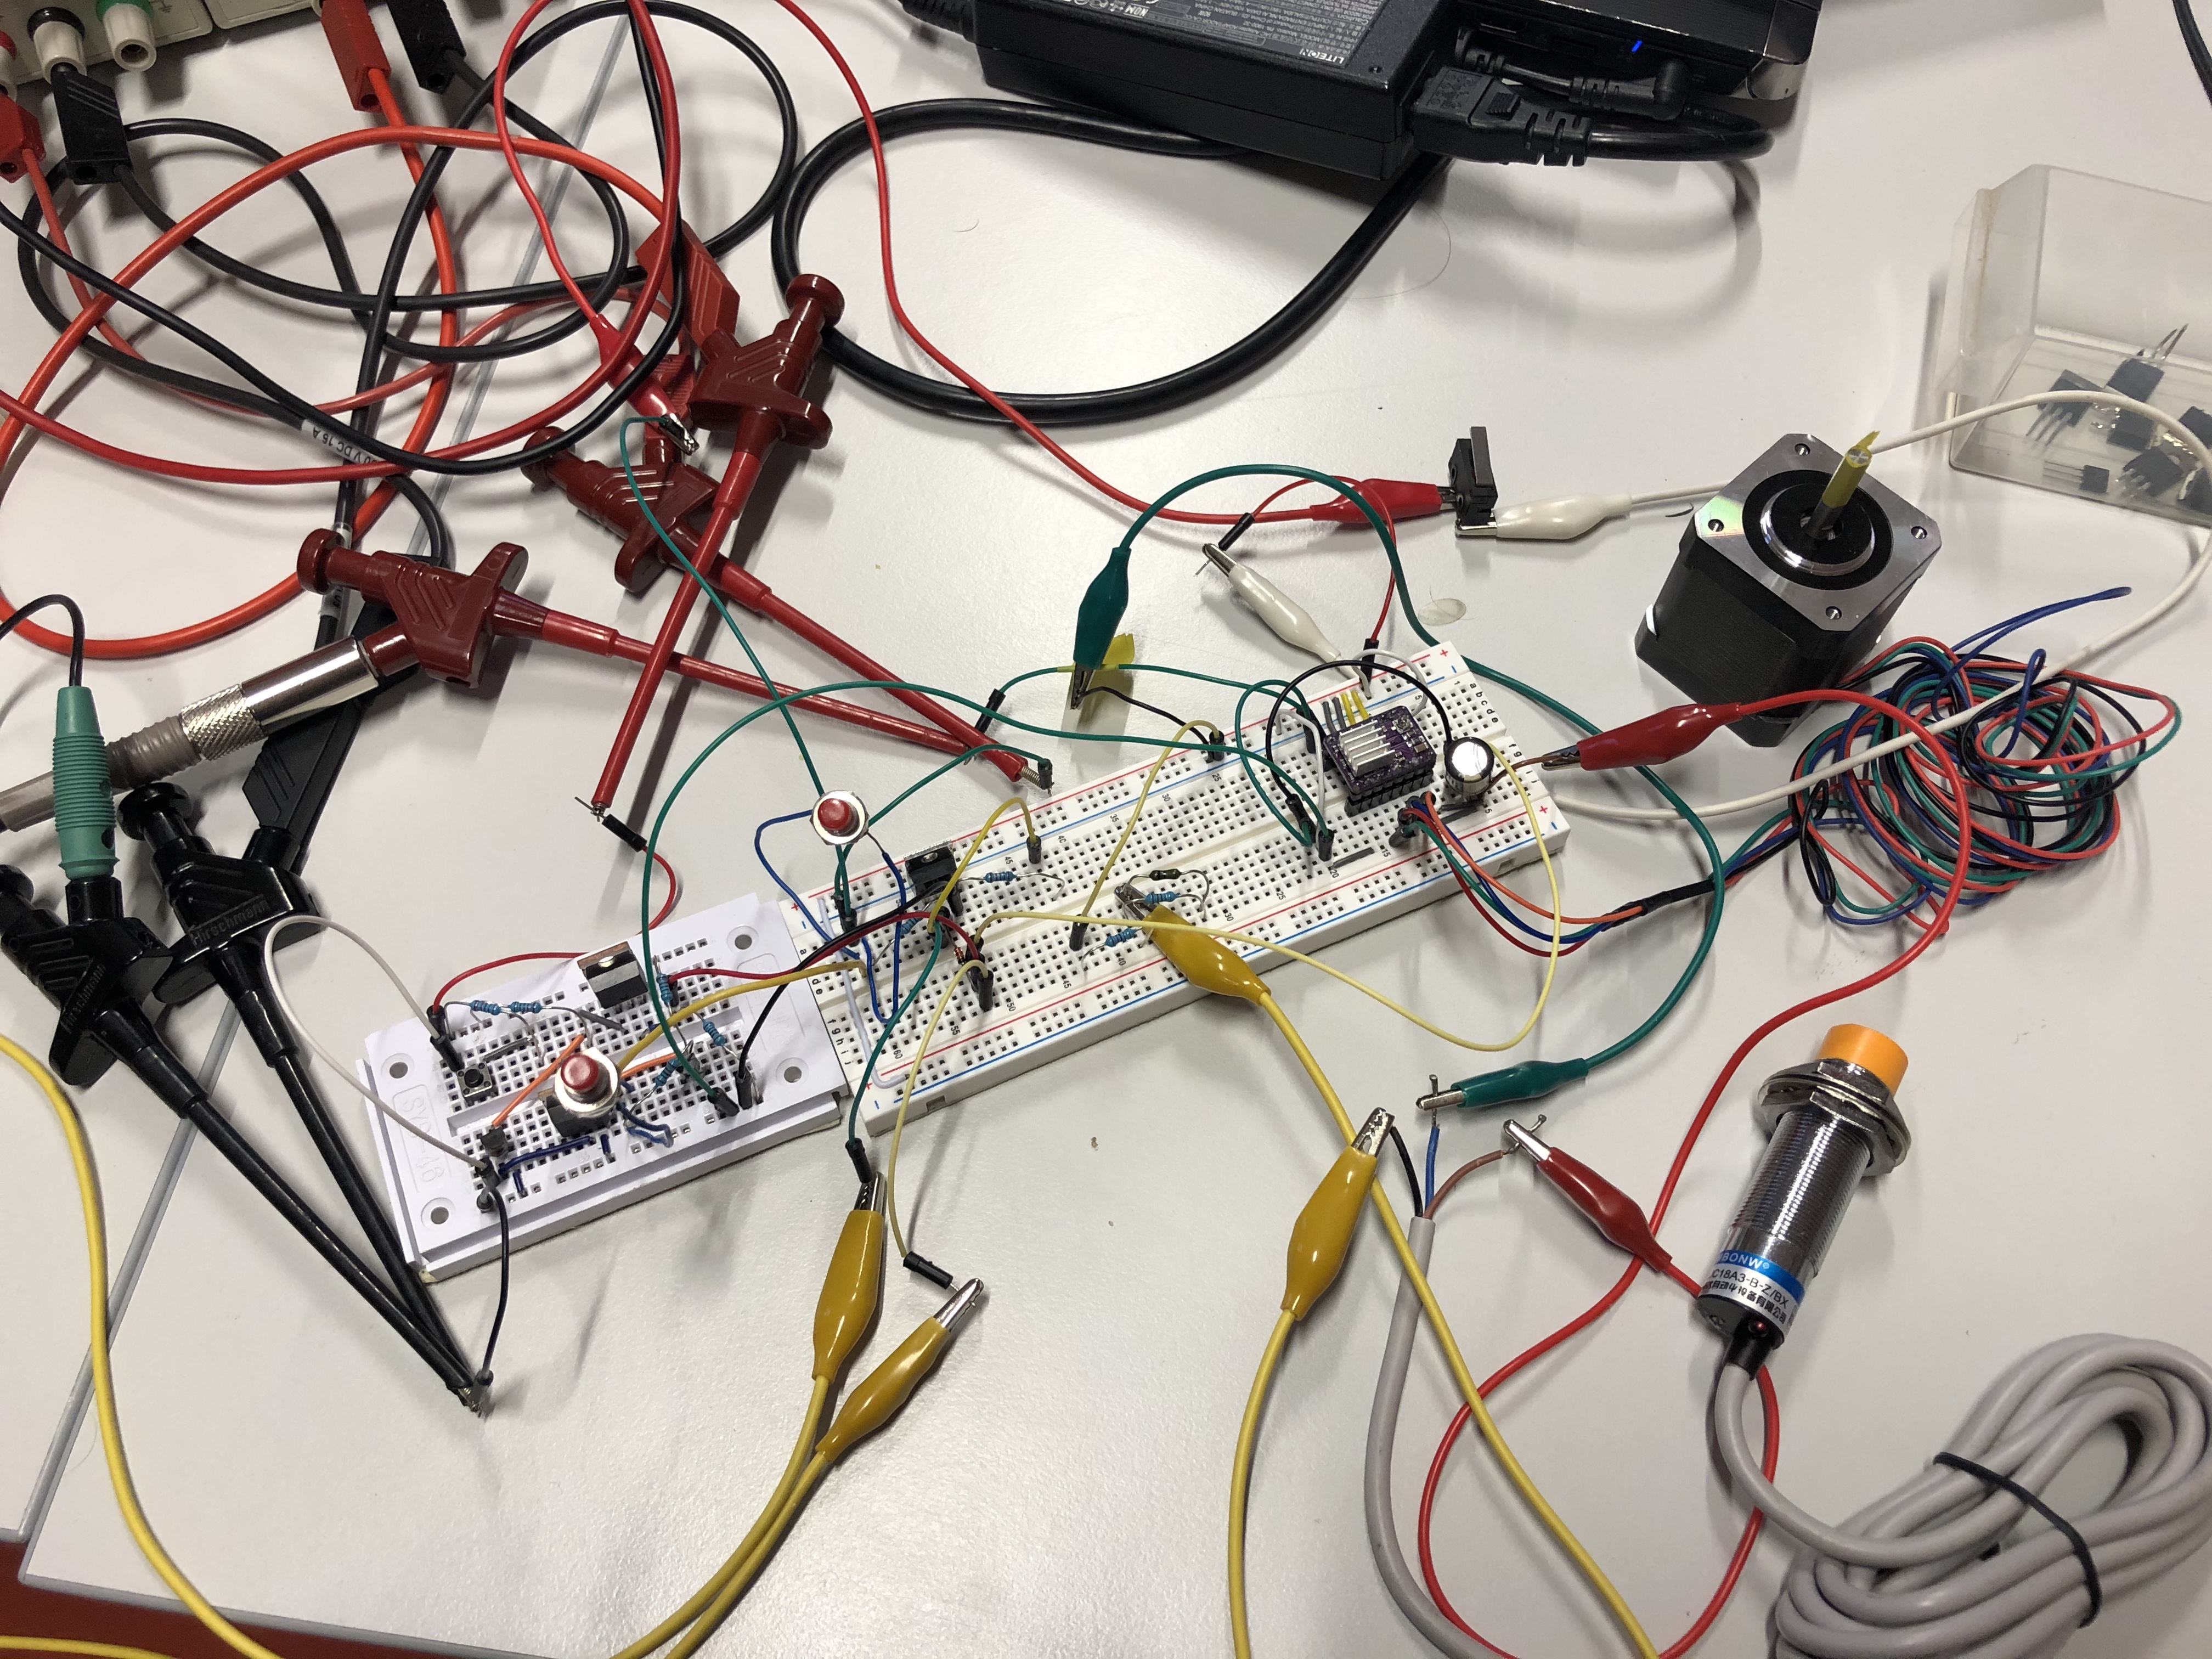
\includegraphics[scale=0.065]{fig/elektro/ErsteSteckbrettVersuche.jpg}
    \caption{Erste Schaltungsrealisierungen in der Praxis}
\end{figure}

\begin{figure}[htb]
    \centering
    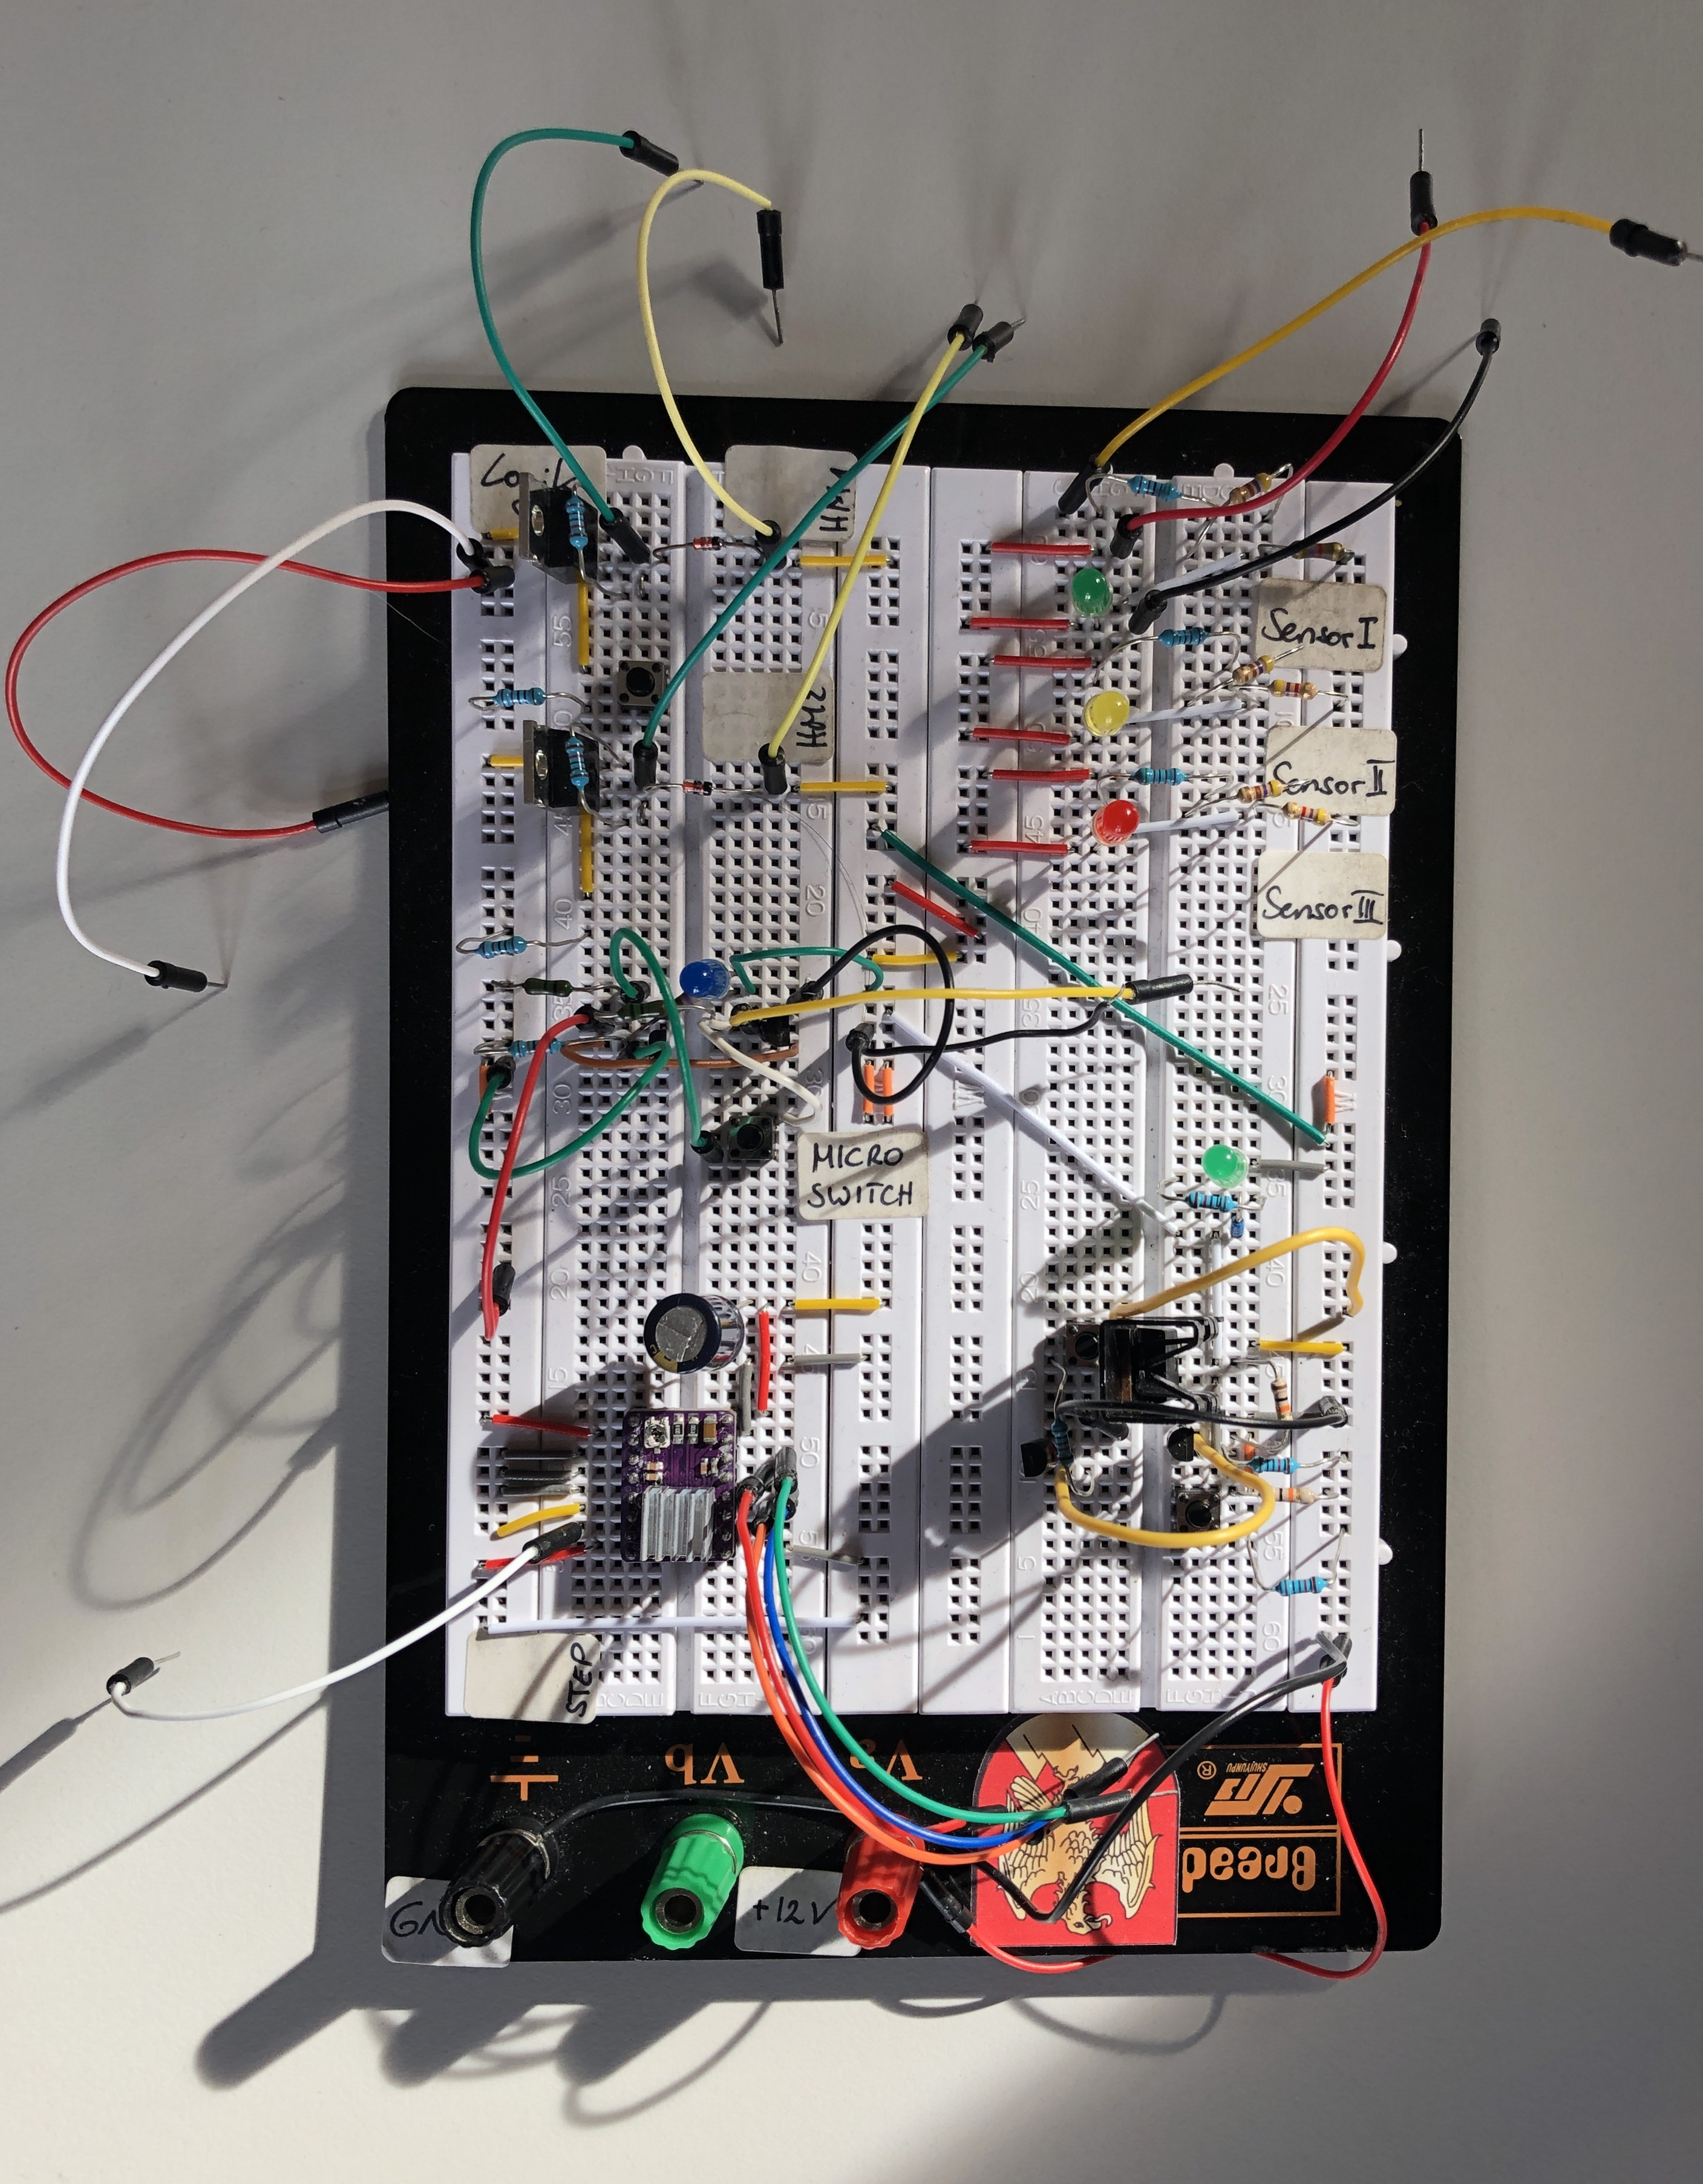
\includegraphics[scale=0.075]{fig/elektro/Steckbrett}
    \caption{Diverse Schaltungen in der Praxis}
\end{figure}

Sobald die Funktionstüchtigkeit einen praktischen Hintergrund angenommen hatte,
war es an der Zeit jegliche Bauteile für die Leiterplatte auszuwählen und zu dimensionieren.

%/\-/\-/\-/\-/\-/\-/\-/\-/\-/\-/\-/\-/\-/\-/\-/\-/\-/\-/\-/\-/\-/\-/\-/\-/\-/\-/\-/\-/\-/\-/\-/\-/\-/\-/\-/\-/\-/\-/\-/\-/\-/\-/\-/\-/\-/\-/\-/\-/\-/\-/\-/\-/\-/\-/\-/\-/\-/\-/\-/\

\newpage
\section{Auswahl der Bauteile}

\subsection{Auswahl der Transistoren}
\subsubsection{P-Kanal MOSFET}

\footfullcite{FDD6637-Datasheet}Als P-Kanal MOSFET traf unsere Wahl auf den FDD6637.
Dieser bringt einen niedrigen Übergangswiderstand vom Drain zur Source  von maximal 0.19m$\Omega$ mit sich.
Außerdem ist dieser dazu in der Lage, eine Spannung von maximal -35V zu schalten und gleichzeitig einen Strom von bis -55A treiben zu können.
Die maximale Gate-Source-Spannung beträgt -25V und die maximale Thresholdvoltage beträgt -3V .
Der FDD6637 besitzt ein TO-252-Gehäuse.

\subsubsection{N-Kanal MOSFET}

\footfullcite{FDN337N-Datasheet}Als N-Kanal MOSFET wählten wir den FDN337N aus, welcher in der Lage ist, Ströme von bis zu 2.2A treiben zu können.
Außerdem ist es diesem möglich, Drain-Source-Spannungen von bis zu 30V zu schalten, was für unsere Anwendung weitaus genügt.
Hinzu kommt noch die wesentliche Tatsache, dass dieser eine niedrige Gate Treshold Voltage von nur max.1V mit sich bringt.
Über Kennlinienwerte im Datenblatt lässt sich erkennen, dass sich der von uns benötigte Strom von 350mA bereits bei 1.25V und 25°C Umgebungstemperatur schalten lässt.
Der FDN337N besitzt eine Gate-Source-Maximalspannung von 8V und ist mit einem SOT-23 Gehäuse erhältlich.

\subsection{Auswahl der Gleichspannungswandler-Peripherie}

\subsubsection{Spule}
\footfullcite{DR127-101-R-Datasheet}Um eine geeignete Spule für den Step-Down Wandler auszuwählen, wurde auf dessen Datenblatt zurückgegriffen.
Über die von uns verwendete Eingangsspannung des Gleichspannungswandlers und den maximal fließenden Strom von 2A
traf unsere Entscheidung über eine Tabelle jener technischen Dokumentation auf eine Spule mit einem Wert von 100µH .
Über die Bedingung einen derartig hohen Strom treiben zu können, fiel unsere Wahl auf die DR127-101-R,
welche die Eigenschaften eines maximalen Gleichspannungsstroms von 3.64A, einen hohen Wirkungsgrad, einen niedrigen magnetischen Sättigungsstrom,
einen niedrigen Widerstandswert, magnetische Schirmung und ein \acs{SMD}-Gehäuse mit sich bringt.

\newpage
\subsubsection{Schottky-Diode}
\footfullcite{MBRD340-Datasheet}Bei der Wahl einer passenden Schottky-Diode wurde ebenfalls auf die technische Dokumentation des Gleichspannungswandlers zurückgegriffen.
Als günstige Lösung wurde die MBRD340 gewählt, da diese einen maxmimalen Strom von 3A standhalten kann und für Spannungen von bis zu 40V geeignet ist.
Eine leichte Montage ist über ihr TO-252 gegeben.

\subsection{Auswahl der Gleichrichter-Dioden}

\footfullcite{RR264M-Datasheet}Als diese Dioden selektierten wir die RR264M, welche einem Strom von 1A standhalten können, was wichtig für die Implementierung an den induktiven Lasten ist.
Zusätzlich besitzt sie die Eigenschaft, einen Spannungsabfall von 0.7V bei einem Strom von 0.01A bei 25°C zu verursachen.
Dies ist essenziell für die Implementierung an jenen Spannungspegelüberwachungspunkten.
Die RR264M besitzen ein SOD-123 Gehäuse.

\subsection{Auswahl der Schottky-Dioden}

\footfullcite{MBR130-Datasheet}Als Schottky-Diode wählten wir die MBR130, welche die Maximalwerte von 1A und 30V mit sich bringt.
Ihr wesentliches Attribut ist der niedrige an ihr abfallende Spannungsabfall von nur 0.25V bei 25°C und 0.1A .
Bei 1A und 25°C beträgt der an ihr vorzufindende Spannungsabfall 0.35V .
Die Eigenschaften des niedrigen Spannungsabfalls in Anbetracht der UNLATCH-Schaltung und der Beschaltung des USB-UART-Converters befürworteten ihren Einsatz.
Über ihr SOD-123 Gehäuse sind sie leicht zu bestücken.

\subsection{Auswahl der Zener-Diode}

\footfullcite[Vgl.]{BZX84-series-Datasheet}Als Zener-Diode selektierten wir die BZX84-C8V2, welche alle gewünschten Eigenschaften und eine Zenerspannung von 8.2V mit sich bringt.
Sie bringt eine maximale Verlustleistung von 250mW, eine Durchlassspannung von 0.9V und ein SOT-23 Gehäuse mit sich.

\subsection{Auswahl sonstiger Bauelemente}

Bei den Bauformen jener Kondensatoren, dessen Wert 100nF oder 22pF beträgt, und aller Leuchtdioden und Widerstände wurde auf 0805er Chips zurückgegriffen,
da sich diese bereits in unserem Besiz befanden und diese eine platzsparende, und dennoch einfach zu lötende Lösung bereitstellten.
Bei der Auswahl der Kondensatoren im µF-Bereich wurde auf SMD-Elektrolytkondensatoren mit einem Diameter von 6 bis 8mm zurückgegriffen.

%/\-/\-/\-/\-/\-/\-/\-/\-/\-/\-/\-/\-/\-/\-/\-/\-/\-/\-/\-/\-/\-/\-/\-/\-/\-/\-/\-/\-/\-/\-/\-/\-/\-/\-/\-/\-/\-/\-/\-/\-/\-/\-/\-/\-/\-/\-/\-/\-/\-/\-/\-/\-/\-/\-/\-/\-/\-/\-/\-/\

\newpage
\section{Leiterplattendesign}

Sobald die Auswahl der Peripherie beendet war, war es an der Zeit ein Design für die geplante Platine in KiCad zu entwerfen.
Als Anforderungen stellten wir uns ein möglichst kompaktes, strukturiertes sowie übersichtliches Design zu erstellen.
Hierzu kamen noch spezifischere Anforderungen, da bei einem Fertigen der Leiterplatte in der schuleigenen Werkstätte nur eingeschränkte Fertigungsparameter gegeben sind.
Zu diesen zählen ein Mindestbohrdurchmesser bei Durchkontaktierungen von 0.6 mm sowie die Tatsache, eine Mindestleiterbahnbreite von 0.2 mm zu verwenden.
Außerdem dürfen keine Durchkontaktierungen unter Bauteilen platziert werden, da bei diesen jeweils ein Leiter per Hand eingelötet werden muss.
Nennenswert ist zudem, dass nur maximal zweilagige Leiterplatten angefertigt werden können.

\subsection{Layoutdesign}

Beim Layoutdesign wurde darauf geachtet, keine \acs{THT} und SMD Bauteile zu vermischen.
Somit wurden diese jeweils auf zwei verschiedenen Layern platziert. \\
Im Laufe der Diplomarbeit entstanden unzählige, verschiedene Layouts, welche die Gründe von ständig neu aufkommenden Ideen, Ausmerzung von Fehlerquellen und Simplifizierungen hatten.
Diese Faktoren machten das Designen eines optimalen Layouts zu einer langwierigen, aber lehrreichen Aufgabe.
Eine falsche Dimensionierung von Bauteilen, Baugruppen und Denkfehler, die das Fertigen erschweren würden, waren hierbei die Hauptfaktoren. \\

Die Breite aller Leiterbahnen wurden auf den maximal fließenden Strom ausgelegt.
Um zu diesen Werten zu kommen, wurde ein Tool angewandt, welches sich in der KiCad Nutzerumgebung finden lässt.
Dieses wendet folgende Formel an: \\

\begin{equation}
    I = K \cdot dT^{0.44} \cdot (W \cdot H)^{0.725}
\end{equation}
wobei
\begin{itemize}
    \item I dem maximal fließenden Strom in Ampere,
    \item K 0.048 für externe oder 0.024 für interne Leiterbahnen,
    \item dT dem Temperaturanstieg über der Umgebungstemperatur in Grad Celsius,
    \item W der Leiterbahndicke in mils und
    \item H der Leiterbahnbreite in mils entspricht.
\end{itemize}

Die folgend zu findenden Abbildungen zeigen die Vorder- und Rückseite des fertigen Leiterplattenlayouts.

\newpage
\subsubsection{Top-Layer}

\begin{figure}[hbt]
    \centering
    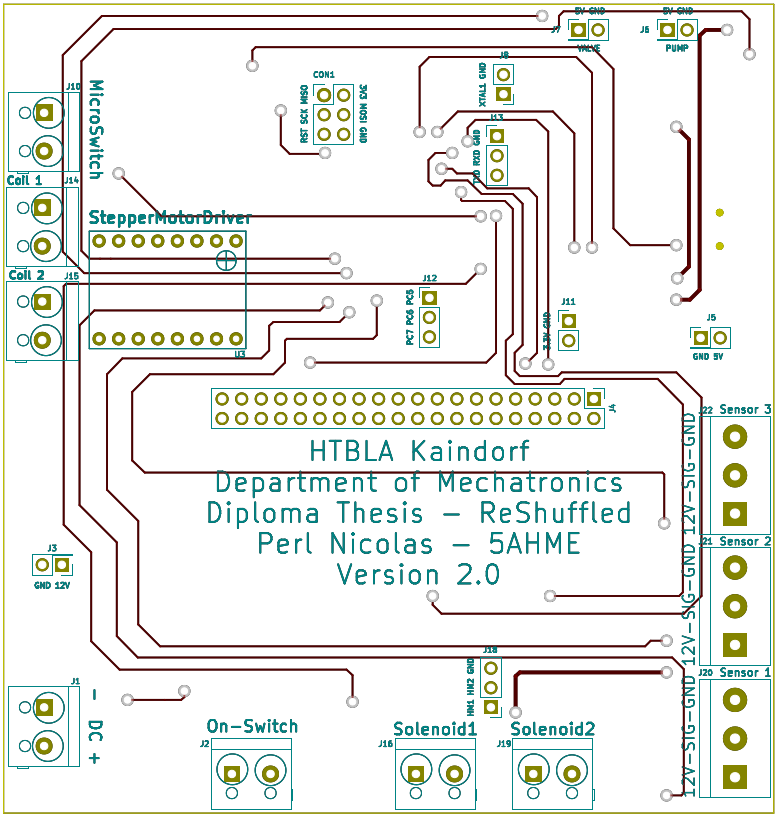
\includegraphics[scale=0.28]{fig/elektro/TopLayer.png}
    \caption{Top-Layer der Leiterplatte}
\end{figure}

\subsubsection{Bottom-Layer}

\begin{figure}[hbt]
    \centering
    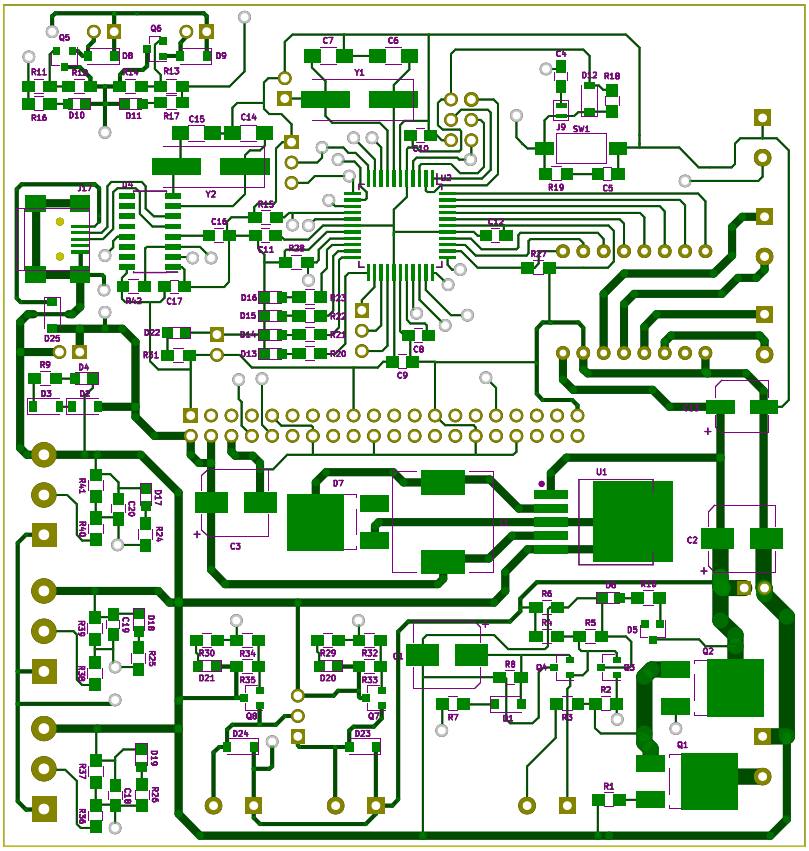
\includegraphics[scale=0.28]{fig/elektro/BotLayer.png}
    \caption{Bottom-Layer der Leiterplatte}
\end{figure}

\newpage
\subsubsection{3D-Ansichten}

\begin{figure}[hb]
    \centering
    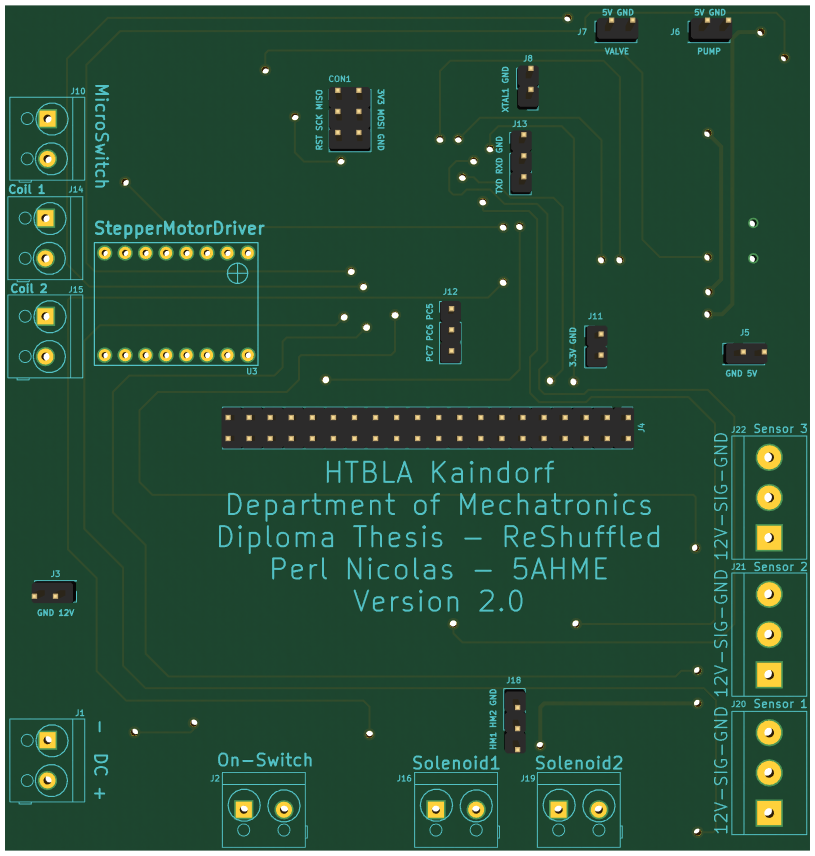
\includegraphics[scale=0.28]{fig/elektro/3DTop.png}
    \caption{3D-Ansicht des Top-Layer}
\end{figure}

\begin{figure}[hb]
    \centering
    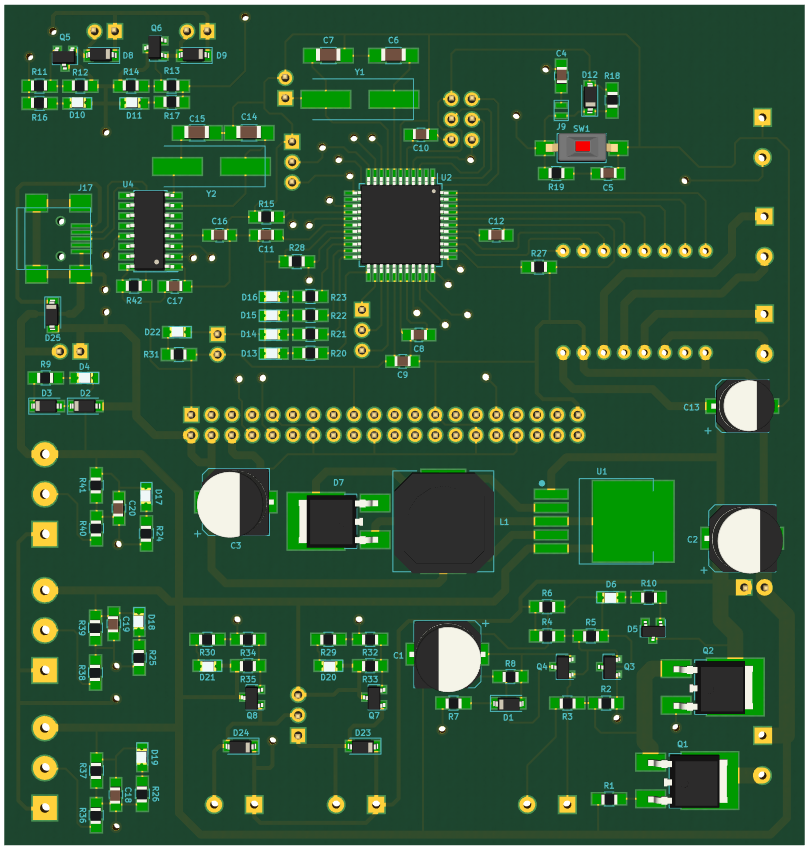
\includegraphics[scale=0.28]{fig/elektro/3DBot.png}
    \caption{3D-Ansicht des Bottom-Layer}
\end{figure}

\newpage
\subsection{Leiterplattenfertigung}

\subsubsection{Prototyping}

Bevor wir fester Überzeugung aller korrekten Funktionen sein konnten, stellten wir uns die Fertigung eines funktionierenden Prototypen als Aufgabe.
Dies hat die Vorteile, etwaige Fehler im Platinenlayout bereits vor der finalen Version zu erkennen und zu korrigieren.
Jener Prototyp wurde in der Werkstätte der HTBLA Kaindorf angefertigt. \\

\textbf{Als Fertigungsschritte sind folgende zu nennen:}

\begin{itemize}
    \item Zu Beginn ist das Layout der Kupfervorderseite und der Kupferückseite jeweils auf ein transparentes Papier mit den bestmöglichen Einstellungen zu drucken.
    Für einen erfolgreichen Druck ist ein Spiegeln der Vorderseite der Platine ein Muss.
    Folgend ist ein Spray zum Verdichten des Toners anzuwenden.
    Aus den zwei Stücken Transparentpapier ist eine Tasche anzufertigen, sodass jegliche Bohrungen genau gegenüberliegen. \\

    \item Zunächst ist die Leiterplatte mithilfe der angefertigten Tasche eine Minute lang in der Belichtungsmaschine unter Vakuum zu belichten. \\

    \item Die beleuchtete Leiterplatte ist anschließend eine Minute lang in ein Natriumhydroxid-Bad zu begeben, um sie zu entwickeln. \\

    \item Folgend ist sie mit heißem Wasser abzuspülen und in ein Natriumpersulfat-Bad zu legen.
    Die Zeitdauer des Verweilens variiert je nach Belastung des Ätzbades.
    In unserem Fall ätzten wir die Leiterplatte 17 Minuten lang. \\

    \item Anschließend ist die Leiterplatte mit heißem Wasser abzuspülen und mit Azeton zu reinigen. \\

    \item Als nächsten Schritt ist sie für einige Minuten in ein Zinnbad zu legen. \\

    \item Nun kann die Leiterplatte ein letztes Mal mit heißem Wasser gespült und mit Fluxclean gereinigt werden.

    \item Letztendlich kann der exakte Zuschnitt und das Bohren durchgeführt werden. \\

    \item Als letzten Schritt kann das Anfertigen von Durchkontaktierungen durch das Einpressen von Nieten sowie das Bestücken der Leiterplatte erfolgen.
\end{itemize}

\subsubsection{Bestückter Prototyp}

Anzumerken ist bei diesem, dass die Idee der Implementierung von einer Pumpe und einem Ventil noch nicht im Raum stand. \\

\begin{figure}[hb]
    \centering
    \includegraphics[scale=0.06]{fig/elektro/PrototypTop.jpg}
    \caption{Draufsicht der Oberseite}
\end{figure}

\begin{figure}[hb]
    \centering
    \includegraphics[scale=0.06]{fig/elektro/PrototypBot.jpg}
    \caption{Draufsicht der Unterseite}
\end{figure}

%/\-/\-/\-/\-/\-/\-/\-/\-/\-/\-/\-/\-/\-/\-/\-/\-/\-/\-/\-/\-/\-/\-/\-/\-/\-/\-/\-/\-/\-/\-/\-/\-/\-/\-/\-/\-/\-/\-/\-/\-/\-/\-/\-/\-/\-/\-/\-/\-/\-/\-/\-/\-/\-/\-/\-/\-/\-/\-/\-/\

\newpage
\section{Verbesserungsmöglichkeiten und Conclusio}
\subsection{Verbesserungsmöglichkeiten}

\subsubsection{Überspannungsschutz}

Sollte man die Versorgung des Raspberry Pi über den Erweiterungsstecker vornehmen, ist ein Überspannungsschutz nicht gegeben.
Eine essenzielle Schutzmaßnahme, um den Raspbbery Pi bei einer zugeführten Überspannung nicht zu beschädigen, wäre einen Überspannungsschutz mithilfe einer Polyfuse und einer Suppresordiode zu implementieren.

\begin{figure}[ht]
    \centering
    \begin{circuitikz}[european, scale = 0.9]
        \draw (0,0) node[anchor=east] {-} to [short, o-*] (4,0);
        \draw (1,3) to [short, -o](0,3)node[anchor=east]{+};
        \draw (4,0) to [/tikz/circuitikz/bipoles/length=1cm,zD-, l_=$D1$, *-*] (4,3);
        \draw (1,3) to[thermistor ptc, l=$PTC$](4,3);
        \draw (4,3) to [short, -o](6,3)node[anchor=west]{+};
        \draw (4,0) to [short, *-o](6,0)node[anchor=west]{-};
        \draw (2,0) to [short, -*](2,0) node[rground]{};
        \draw (0,2.8) -- node[left] {$U_\mathrm{e}$}node[sloped,currarrow,pos=1] {}(0,0.2);
        \draw (6,2.8) -- node[right] {$U_\mathrm{a}$}node[sloped,currarrow,pos=1] {}(6,0.2);
    \end{circuitikz}
    \caption{Überspannungsschutz mit PTC}
\end{figure}

Sollte die Eingangsspannung die bauelementspezifische Spannungsschwelle der Supressordiode überschreiten, wird diese leitend.
Infolgedessen wird der Strom des Spannungsimpulses an der zu schützenden Peripherie vorbeigeführt.
Aufgrund dessen kann sich keine zerstörerische Spannung oberhalb des Suppressors aufbauen.
Der nun rasant steigende Strom bewirkt ein Steigen der Leitungstemperatur.
Aus diesem Grunde heraus steigt auch der Widerstand des Thermistors, weshalb dieser den Strom begrenz und er somit auf ein Minimum zurückfällt.

Diese Schaltung bringt die positive Tatsache mit sich, dass sie sich im Grundzustand, bis auf den niedrigen Leakagestrom der Diode und den geringen Widerstand des PTC, neutral verhält.
Außerdem führt eine Auslösung der Schutzschaltung zu keiner Zerstörung von Bauteilen.
Es muss lediglich auf das Abkühlen des PTC gewartet werden.

Diese Schaltung konkret auf unsere Anwendung nutzbar gemacht, wären die Komponenten wie folgt zu wählen:
\begin{itemize}
    \item PTC als MF-MSMF250/16X
    \item D1 als SMBJ5.A/CA
\end{itemize}

\footfullcite{MF-MSMF250-Datasheet}Die wiederverwendbare Sicherung MF-MSMF200 hält eine maximale Spannung von 8V und einen Haltestrom von 2A bei 23°C Umgebungstemperatur aus.
Im Grundzustand beträgt der Widerstand bei 23°C zwischen 0.02$\Omega$ und 0.08$\Omega$ .
Die Auslösezeit bei einem Strom von 8A bei 23°C beträgt maximal 3 Sekunden.
\newpage
\footfullcite{SMBJ5.A-Datasheet}Die als SMD ausgeführte Suppressordiode SMBJ5.A/CA bringt eine Breakdown Voltage von mindestens 6.4V bis maximal 6.74V mit sich.
Sie verfügt über einen niedrigen Leakage-Strom von 0.2µA bei 25°C und hält einer Spitzenimpulsverlustleistung von 600W stand.

\subsubsection{Einzelne weitere Verbessungsmöglichkeiten}

Als Ziel, ein langlebiges Produkt zu designen, sollte bei dem USB-Stecker auf einen THT-Baustein zurückgegriffen werden,
da erhöhte Kräfte beim Abstecken die Festigkeit des SMD-Bausteins auf lange Zeit hin verringern.
Um außerdem die Komfortabilität zu erhöhen, sollten wartungsfreundlichere Sensoren in Betracht gezogen werden. \\

Um ein Produkt mit höherer Qualität zu erlangen, sollte die Möglichkeit einer professionellen Leiterplattenfertigung abgewägt werden,
welche die Attribute einer betrachtlicheren Optik, einer beidseitigen Kennzeichnung der Bauteilreferenzen sowie kleinere Durchkontaktierungen mit sich bringen würde. \\

Damit bei der UNLATCH-Schaltung genaue Zeitkonstanten zur Berechnung herangezogen werden können, müssen diese gemessen werden.
Konkret bedeutet das, ein Oszilloskop mit vier Kanälen zu verwenden und
die Spannungsverläufe am UNLATCH-Ausgang des µC, der 12V-Leitung, der 5V-Leitung sowie am Drain Anschluss des N-Kanal MOSFET Q3 zu messen (siehe \autoref{fig:SoftLatchingCircuit}).

\subsection{Zusammenfassung}

Das Ziel dieser Arbeit war, eine elektronische Steuereinheit zu kreieren, welche in der Lage ist, jegliche Aktoren anzusteuern, Sensoren einzulesen und mit einem Raspberry Pi Information auszutauschen.
Eingehende Information soll über den vorgesehenen Mikrocontroller verarbeitet, und Prozesse über diesen ausgeführt werden. \\

Mit diesen Anforderungen wurde ein Schaltplan erstellt und eine Platine geplant, entworfen, gefertigt und bestückt.
Durch ausführliches Testen wurden Fehlerquellen und einzelne Mängel korrigiert, sodass ein weitgehend funktionstüchtiger Prototyp zu Stande kam.\\

\subsection{Conclusio}

Nach Ansicht des Autors hat dieser viel Wissen in den Bereichen Projektorganisation, Prototyping und Hardwaredesign erlangt.
Das durch diese Arbeit erworbene Fachwissen in verschiedenen Softwareprodukten,
in Schaltungsdimensionierungen allgemein sowie in der Praxis gemachte Fehler erachtet der Autor als essenziell und wegweisend für die Zukunft.

%/\-/\-/\-/\-/\-/\-/\-/\-/\-/\-/\-/\-/\-/\-/\-/\-/\-/\-/\-/\-/\-/\-/\-/\-/\-/\-/\-/\-/\-/\-/\-/\-/\-/\-/\-/\-/\-/\-/\-/\-/\-/\-/\-/\-/\-/\-/\-/\-/\-/\-/\-/\-/\-/\-/\-/\-/\-/\-/\-/\

    %@COPYRIGHT VOLLMAIER ALOIS
%@COPYRIGHT VOLLMAIER ALOIS
\definecolor{hellgrau}{RGB}{230, 230, 230}
\lohead{Vollmaier Alois}
\chapter{Informatik}\label{ch:informatik}

\section{Allgemeines}\label{sec:einleitung}
Im folgenden Projektteil werden die Kernbestandteile sowie der nähere Aufbau des informatischen Bereichs dieser Arbeit gezeigt.
Weiters werden wesentliche Elemente der Inbetriebnahme der Maschine dokumentiert und zusammengefasst.
Die Aufteilung dieses XX seitigen Kapitels überstreckt sich über alle signifikanten Teile der grafischen Oberfläche, bezeichnet als \textbf{Frontend}, bis hin zu den im Hintergrund arbeitenden Funktionen, welche als \textbf{Backend} zusammengefasst werden.
Auch wird gezeigt, wie einige Teile der \textbf{Hardwarenahen-Programmierung} funktionieren und wie diese mit der Steuerelektronik zusammenarbeiten.
Folglich werden am Schluss der Verlauf der \textbf{Testing-Phase} sowie die Zusammensetzung des \textbf{Teilaufbaus} erläutert.

\section{Zeitplan}\label{sec:zeitplan}
\begin{figure}[hbt!]
    \centering
    \scalebox{0.57}{
    \begin{ganttchart}[
    hgrid style/.style={black, dotted},
    calendar week text={\currentweek},
    vgrid={*6{white, dotted}, *1{black, dashed}},
    x unit=1mm,
    group label font=\bfseries \Large,
    y unit chart=9mm,
    y unit title=12mm,
    time slot format=isodate,
    time slot unit=year
    link/.style={->, thick}
    ]{2019-09-2}{2020-03-15}
        \gantttitlecalendar{year, month=name, week}\\

        \ganttgroup[
        group/.append style={fill=red}
        ]{Backend-Programmierung}{2019-09-02}{2019-11-15}\\ [grid]
        \ganttbar[
        bar/.append style={pattern=north east lines},
        name=KonzeptplanungBack
        ]{Konzeptplanung}{2019-09-02}{2019-09-25}\\ [grid]
        \ganttbar[
        bar/.append style={pattern=north east lines},
        name=Einrichtung - Arbeitsumgebung
        ]{Einrichtung - Arbeitsumgebung}{2019-09-15}{2019-10-1}\\ [grid]
        \ganttbar[
        bar/.append style={pattern=north east lines},
        name=Start-ProgrammierungBack
        ]{Programmierung}{2019-10-05}{2019-11-15}

        \ganttnewline[thick, black]

        \ganttgroup[
        group/.append style={fill=blue}
        ]{Frontend-Programmierung}{2019-11-15}{2020-1-09}\\ [grid]
        \ganttbar[
        bar/.append style={pattern=north east lines},
        name=KonzeptplanungFront
        ]{Konzeptplanung}{2019-11-15}{2019-11-31}\\ [grid]

        \ganttbar[
        bar/.append style={pattern=north east lines},
        name=KonzeptplanungFront
        ]{Anfertigen von Mockup-Skizzen}{2019-11-25}{2019-11-31}\\ [grid]

        \ganttbar[
        bar/.append style={pattern=north east lines},
        name=Start-ProgrammierungFront
        ]{Programmierung}{2019-12-2}{2019-12-22}

        \ganttnewline[thick, black]

        \ganttgroup[
        group/.append style={fill=green}
        ]{Hardwarenahe-Programmierung}{2019-31-31}{2020-2-12}\\ [grid]
        \ganttbar[
        bar/.append style={pattern=north east lines},
        name=KonzeptplanungHard
        ]{Konzeptplanung}{2019-12-31}{2020-1-10}\\ [grid]


        \ganttbar[
        bar/.append style={pattern=north east lines},
        name=Start-ProgrammierungHard
        ]{Programmierung}{2020-1-10}{2020-1-31}

        \ganttnewline[thick, black]

        \ganttgroup[
        group/.append style={fill=green}
        ]{Testen - Aufbauen}{2019-12-22}{2020-02-01}\\ [grid]

        \ganttbar[
        bar/.append style={pattern=north east lines},
        name=Teilaufbau
        ]{Teilaufbau Anfertigung}{2019-12-22}{2020-1-09}\\

        \ganttbar[
        bar/.append style={pattern=north east lines},
        name=Frontend-Testing-Phase
        ]{Frontend-Testing-Phase}{2019-12-31}{2020-1-15}\\

        \ganttbar[
        bar/.append style={pattern=north east lines},
        name=Serial-Testing-Phase
        ]{Serial-Testing-Phase}{2020-1-31}{2020-2-15}

    \end{ganttchart}
    }
    \caption{Zeitplanung - Informatik}
\end{figure}
Das hier gezeigte Bild illustriert, wie der Projektzeitraum aufgeteilt wird.
Um das Zeitfenster des Projekts nicht zu verzögern werden folgende Meilensteine in den Zeitplan implementiert:
\begin{enumerate}
    \item xx.xx.xxxx - Aufgabe XX
    \item xx.xx.xxxx - Aufgabe XX
    \item xx.xx.xxxx - Aufgabe XX
\end{enumerate}
\section{Anforderungen und Ziele}\label{sec:anforderungen-und-ziele}
\subsection{Fronted-Programmierung}\label{subsec:fronted-programmierung}
Im Allgemeinen besteht das Ziel darin, eine benutzerfreundliche grafische Bedienoberfläche zu realisieren, welche schlussendlich im Betrieb der Maschine auf einem 7" Display angezeigt werden soll.
Auf diesem Interface soll es möglich sein, die Steuerung der Maschine zu übernehmen.
Die Möglichkeiten des Benutzers, die Maschine zu bedienen sollen folgende Kernpunkte beinhalten:
\begin{enumerate}
    \item Ausgabe von einzelnen Spielkarten
    \item Konfigurierung von Spielmodi, welche Einstellungen zum Spiel beinhalten
    \item Das Zählen von Punkten und dessen Visualisierung am Display
    \item Ausschalten der Maschine
    \item Übersicht aller vergangenen Spiele
\end{enumerate}
Die wesentliche Anforderung, die Oberfläche einfach und schlicht zu halten, soll im Projekt berücksichtigt werden.
Grundsätzlich steht die sogenannte \textbf{User-Experience}, welche alle Aspekte der Eindrücke eines Nutzers bei der Interaktion mit einem Produkt beschreibt, sowie die \textbf{Funktionalität} bei der Programmierung im Vordergrund.
Um dies zu gewährleisten, sollte eine Voruntersuchung vollzogen werden.

\subsection{Backend-Programmierung}\label{subsec:backend-programmierung}
Wie in der Einleitung bereits erwähnt besteht das Backend aus Tätigkeiten, welche im Hintergrund abgearbeitet werden.
Diese Aufgaben umfassen die Kommunikation des Raspberry PI mit der Ansteuerplatine sowie dem Simulator.

Auch soll im Hintergrund eine sogenannte LOG-Datei, welche wichtige Aktionen protokolliert, automatisch vom Programm generiert werden.
Diese Datei kann z.B. \ beim Debugging-Vorgang notwendig sein bzw. \ dem Entwickler dabei unterstützen, was eine enorme Zeitersparnis mit sich bringt.

Um etwaige Einstellungen der Seriellen Schnittstelle sowie die Definition der Pfade für verschiedene Dateien außerhalb des Programmes vorzunehmen, ist es auch nötig, eine Konfigurationsdatei zu erstellen, welche nach jedem Start vom Programm eingelesen wird.
Mit dieser sogenannten Config-Datei wird auch die Möglichkeit geschaffen, weitere Informationen der Anwendung auch nach einem Neustart der Maschine zu speichern.

Diese hiermit geschaffene Datenpersistenz kommt dem Programm auch bei der zukünftigen Speicherung der Spielmodi oder etwaigen Statistik-Dateien zugute.
Bei einer Realisierung einer Statistik-Datei sollte der Name des ausgewählten Spielmodis, dessen Hintergrundinformationen, Spielernamen und Punkteanzahl Kernbestandteil sein.

Ein weiteres Ziel ist die Internationalisierung der gesamten Software.
Soll eine Software in verschiedenen Ländern eingesetzt werden, ist eine Internationalisierung ein wichtiger Bestandteil der User Experience.
In unserem Fall ist es lediglich notwendig, alle angezeigten Texte zu übersetzen, da keine weiteren Informationen vorhanden sind.

\subsection{Hardwarenahe-Programmierung}\label{subsec:hardwarenahe-programmierung}
Ein weiterer Punkt des Projekts ist die Hardwarenahe-Programmierung.
Aufgrund der Tatsache, das die verwendete Ansteuerplatine über einen ATmega 324PA verfügt, ist es notwendig, eine Programmierung dieses Mikrocontrollers durchzuführen.
Als Basis dafür dienen ankommenden Befehle über der seriellen Schnittstelle.
Ziel ist es also, diese serielle Kommunikation auf dem Mikrocontroller auszuprogrammieren.

\section{Projektspezifische Voruntersuchung}\label{sec:projektspezifische-voruntersuchung}
Damit dem Programmierprozess nichts mehr im Wege steht, ist es notwendig, einige Voruntersuchungen durchzuführen.
Folgend werden einige grundlegende Fragen geklärt und näher erläutert.
\subsection{Auswahl der Arbeitsumgebung}\label{subsec:auswahl-der-arbeitsumgebung}
Das Bearbeiten von Code spielt bei der Programmierung eine elementare Rolle.
Dadurch muss, bevor mit dem Programmierprozess gestartet wird, eine passende IDE ausgewählt werden, welche alle vom Benutzer gestellten Anforderungen erfüllt.
In unserem Fall sind diese im Speziellen:
\begin{enumerate}
    \item Möglichkeiten der Programmierung sowie dem Debuggen eines Remote-Rechners
    \item Nötigsten Features beinhalten
    \item Grafisch Ansprechend
\end{enumerate}
Einer der wichtigsten Punkte dieser Aufzählung ist dabei jedoch die Möglichkeit, Remote-Geräte zu debuggen.
Debugging selbst hilft dem Entwickler bei der Fehlersuche.
Mithilfe der Möglichkeit, das Programm schrittweise auszuführen, ist es auch möglich, die aktelle Wertebelegung von Variablen zu überprüfen.
Dadurch erspart dies enorme Zeit bei der Programmierung.
In unserem Fall ist das Endgerät jedoch nicht der PC, sondern ein Raspberry PI, welcher mit dem Netzwerk über Ethernet verbunden ist.
Es erfordert aber nun die Möglichkeit, das Gerät über das Netzwerk zu debuggen.
\subsubsection{Apache-Netbeans}
Die Netbeans-IDE, bereitgestellt von der Firma Apache, ist eine Open-Source Entwicklungsumgebung, welche selbst in der Programmiersprache Java geschrieben wurde und damit plattformunabhängig ist.
Primär wurde sie entwickelt, um Programme in der Programmiersprache Java zu erstellen.\\
Große Vorteile bringt diese IDE im Bereich der Remote-Programmierung mit sich.
Die Möglichkeit, eine Remote-Plattform einzurichten wurde einfach gelöst und das Arbeiten verläuft meist ohne Probleme.
Auch das einfache Einbinden von Plugins und Bibliotheken zählt zu den Hauptvorteilen von Netbeans.
\subsubsection{Intellij IDEA}
Eine kostenpflichtige Alternative zu Netbeans ist Intellij.
Aufgrund der komplizierten Einrichtung eines Remote-Systems, sowie dessen Handhabung im täglichen Arbeitsprozess wurde deutlich, dass Netbeans im wichtigsten Kriterium besser abschneidet.
Jedoch bring Intellij auch einige Vorteile mit sich.
\begin{enumerate}
    \item Flüssigere Bedienung
    \item Wirkt durchdachter
    \item Zentralere Verwaltung von Plugins
\end{enumerate}
\subsubsection{Fazit}
Natürlich ist es meist Ansichtssache, für welche IDE man sich entscheidet doch in Anbetracht der Vorteile von Netbeans gegenüber Intellij im Bereich der Remote-Programmierung, wurde auch diese IDE für den zukünftigen Arbeitsprozess gewählt.
\subsection{Auswahl des GUI-Frameworks}\label{subsec:auswahl-des-gui-frameworks}
Die Auswahl des für die Anwendung am besten geeigneten GUI-Frameworks, spielt eine wesentliche Rolle in der programmierung von grafischen Anwendungen.
Diese Frameworks stellen meist alle Elemente zur Erstellung einer GUI bereit.
Diese sind z.B.\ Knöpfe, Listen und Textfelder mit denen der Benutzer interagieren kann.
\subsubsection{Swing}
Das bereits in der Standard-Java-Bibliothek verfügbare Java Swing bietet die Möglichkeit komplexe Oberflächen zu erstellen.
Der Aufwand zur Einrichtung hält sich in Grenzen denn im Vergleich zu Java-FX muss hier nicht extern in einem eigenen Programm gearbeitet werden, um die GUI zu erstellen.
Aufgrund der Verfügbarkeit von Java Swing in der Java Bibliothek bieten alle IDE's die Möglichkeit zur erstellung von Oberflächen.
Das etwas veraltete und lieblose Look and Feel von Java Swing brachte uns zur Entscheidung, den Nachfolger, nämlich Java FX, zu verwenden.
\subsubsection{JavaFX}\label{sssec: JavaFX}
JavaFX ist ein GUI-Framework, welches oft als Java-Swing nachfolger betitelt wird.
Hierbei werden im Vergleich zu Java Swing nicht alle GUI Elemente in einer Datei beschrieben, was die Übersichtlichkeit beeinträchtigt, sondern die Beschreibung geschieht in externen FXML-Dateien.
Die Basis dieser FXML-Dateien ist XML, eine Sprache zur Darstellung von Daten in einem von Menschen lesbaren Format.
Näher wird dieses Format im \autoref{subsec:datenformate-in-java-fx} erklärt.
Der logische Code hinter der GUI befindet sich jedoch nicht in diesen Dateien, sondern in eigenen Controller-Klassen, welche mit der GUI verknüpft sind.
Dies bringt enorme Vorteile mit sich, denn die strikte Trennung zwischen beschreibenden Elementen der GUI
und dem dahinter stehenden Code ist dadurch möglich.
Benennen darf sich dieses Designkonzept Model-View-Controller. \autoref{subsec:entwurfsmuster-mvc}\\
Auch bieter Java FX die Möglichkeit, separate Stylesheets, also Dokumente, in welchen das Aussehen von Elementen beschrieben wird, zu erstellen.
Diese verbessern das sogenannte Look and Feel drastisch.\\\\
Im Gegensatz zu Java-Swing muss man als Programmierer hier auch nicht die \lstinline[style=java]{Stage} mithilfe von \lstinline[style=java]{new JFrame()} erzeugen, sondern dies wird von JavaFX automatisch erledigt um diese danach der Methode \lstinline[style=java]{start(Stage)} zu übergeben.
So werden einem viele Schnritte beim Start durch die Methode \lstinline[style=java]{launch()} abgenommen.
% @formatter:off
\begin{lstlisting}[style=java,caption=Java-Codebeispiel,label=commThreadSync]
  public static void main(final String[] args)
  {
    launch(args);
  }
\end{lstlisting}
% @formatter:on
Innerhalb der \lstinline[style=java]{Stage} wird die Oberfläche in eine \lstinline[style=java]{Scene} und verschiedenen \lstinline[style=java]{Nodes} eingeteilt, wobei \lstinline[style=java]{Nodes} etwaige Controls und die \lstinline[style=java]{Scene} den gemeinsamen Container dieser Controls darstellt.
\begin{figure}[H]
    \centering
    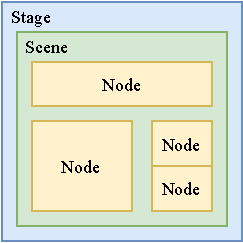
\includegraphics[width=0.3\textwidth]{fig/ainf/JavaFXStageSceneNode.pdf}
    \caption{JavaFX Stage-Scene-Node Übersicht}
    \label{fig:Stage-Scene-Node}
\end{figure}
\subsubsection{Fazit}
Im Großen und Ganzen fiel aufgrund des großen Spektrums an Möglichkeiten, die Wahl auf das JavaFX-Framework.
Dieses fordert jedoch eine Einarbeitungsphase, welche aber keine Auswirkung auf den Umfang des Projekts hat.
\subsection{Projektorganisation}\label{subsec:projektorganisation}
\subsubsection{Projektstruktur in Netbeans}
Eine einheitliche Formatierung und Namensgebung ein Kernbestandteil einer gelungenen Projektplanung.
Dies führt zu einer leichteren Orientierung in fremden aber auch in eigenen Projekten.
Um die Übersichtlichkeit eines Projektes zu verbessern wird nach einer klar definierten Projektstruktur gearbeitet.
Anhand der folgenden Grafik kann die Projektstruktur dieses Projektes abgelesen werden:
\begin{figure}[H]
    \begin{center}
        \begin{forest}
            for tree={
            font=\ttfamily,
            grow'=0,
            child anchor=west,
            parent anchor=south,
            anchor=west,
            calign=first,
            edge path={
            \noexpand\path [draw, \forestoption{edge}]
            (!u.south west) +(7.5pt,0) |- node[fill,inner sep=1.25pt] {} (.child anchor)\forestoption{edge label};
            },
            before typesetting nodes={
            if n=1
            {insert before={[,phantom]}}
            {}
            },
            fit=band,
            before computing xy={l=15pt},
            }
            [<project-root>
            [src
            [data
            ]
            [exception
            ]
            [gui
            ]
            [logging
            ]
            [main
            ]
            [serial
            ]
            [util
            ]
            ]
            [lib]
            [config]
            ]
        \end{forest}
    \end{center}
    \caption{Projektstruktur}
\end{figure}
Der Kopf dieser Struktur beschreibt den Ordner mit dem Namen des Projekts.
Dieser wird auch \lstinline{root-directory} genannt, und ist selbst kein Package.
Auch die Trennung von Sourcecode und externen Dateien spielt eine wesentliche Rolle.
Dadurch erfolgt darunter die Aufteilung in die Ordner \lstinline{src}, \lstinline{lib}, \lstinline{config}.
\\\\
\textbf{Sourcecode}
\\
Im Ordner \lstinline{src} befindet sich der gesamte Sourcecode, wobei in diesem auch wieder eine Aufteilung in Packages erfolgt.
Diese benennen sich in unserem Fall \lstinline{data}, \lstinline{exception}, \lstinline{gui}, \lstinline{logging}, \lstinline{main}, \lstinline{serial}, und \lstinline{util}.
\\\\
\textbf{Bibliotheken}
\\
Oft werden externe Bibliotheken verwendet, welche im Ordner \lstinline{lib} gesammelt werden.
Dabei erleichtert diese Verzeichnishirachie die übersichtlichkeit aller verwendeten Bibliotheken und dessen Versionen.
\\\\
\textbf{Konfigurationsdateien}
\\
In unserem Fall ist es auch notwendig, einen Ordner explizit für Konfigurationsdateien vorzusehen.
Dort können Textresourcen für Sprachvarianten und Konfigurationsdateien für etwaige Aufgaben abgelegt werden.

\subsubsection{Projektstruktur für Maven und Gradle}
Das zuvor genannte Layout der Projekthrachie eignet sich gut für viele Projekte.
Jedoch zeigen sich nach und nach einige Schwachstellen an diesem System.

Einerseits ist das aufwendige Erstellen dieser Hirachie ein Punkt, welcher nicht unerwähnt bleiben soll.
Auch besteht ein Risiko zur Inkonstistenz bei der Namensgebung von Packages oder Bibliotheken. \\
Im Vergleich dazu, schreibt Maven und Gradle eine klar definierte Projektstruktur vor.

\begin{figure}[H]
    \begin{center}
        \begin{forest}
            for tree={
            font=\ttfamily,
            grow'=0,
            child anchor=west,
            parent anchor=south,
            anchor=west,
            calign=first,
            edge path={
            \noexpand\path [draw, \forestoption{edge}]
            (!u.south west) +(7.5pt,0) |- node[fill,inner sep=1.25pt] {} (.child anchor)\forestoption{edge label};
            },
            before typesetting nodes={
            if n=1
            {insert before={[,phantom]}}
            {}
            },
            fit=band,
            before computing xy={l=15pt},
            }
            [<project-root>
            [src
            [main
            [java
            [resources]
            ]
            ]
            [test
            [java
            [resources]
            ]
            ]
            ]
            ]
        \end{forest}
    \end{center}
    \caption{Projektstruktur}
\end{figure}
Trotz alledem wurde auf die althergebrachte Version der Projekterstellung gesetzt.
Grund dafür ist widerum die fehlende Möglichkeit, Remote-Debugging durchzuführen.
Natürlich wäre eine Umstellung in einem finalen Release denkbar.

\section{Grundlagen}\label{sec:grundlagen}
\subsection{Entwurfsmuster Singelton}\label{subsec:entwurdsmuster-singelton}
\subsubsection{Beschreibung}
Das Erzeugungsmuster namens Singelton dient dazu, die Einzigartigkeit eines Objekts sicherzustellen.
Das bedeutet eine Instanz des Objektes ist nur genau einmal im Speicher vorhanden.
Auch bietet eine Klasse, welche nach dem Singelton-Pattern erzeugt wurde, einen globalen Zugriffspunkt über das gesamte Programm.
\subsubsection{Struktur}
Realisiert wird dies durch einen privaten Kontruktor, denn wo keine Zugriffsberechtigung von außen herrscht, kann auch kein Objekt erstellt werden.
Dies bedeutet es liegt eine Kapselung des Konstruktionsprozesses innerhalb der Klasse vor.
Die einzige Möglichkeit, eine Instanz zu erstellen, liefert die statische Methode \lstinline{createInstance()}.
Wurde einmal eine Instanz erzeugt, also der private Konstruktor durch \lstinline{createInstance()} aufgerufen, wird diese erzeugte Instanz in einem statischen Attribut gespeichert.\\
\begin{figure}[H]
    \centering
    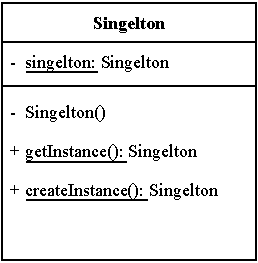
\includegraphics[width=0.25\textwidth]{fig/ainf/Singelton.pdf}
    \caption{UML-Diagramm Singelton}
\end{figure}
Natürlich wird auch ein Zugriffspunkt auf dieses Attribut benötigt.
Implementiert wird dies durch eine weitere statische Methode namens \lstinline{getInstance()}.
Diese Methode ist der einzige Zugriffspunkt auf die Instanz.
\subsubsection{Beispiel}
Das folgende \textit{\autoref{Singelton Code}}, entnommen aus dem \textit{\autoref{subsec:konfiguration}}, zeigt wie Singelton angewendet werden kann.
\lstinputlisting[firstline=21, lastline=42, style=java,caption=Singelton Codebeispiel,label=Singelton Code]{src/data/config/Config.java}
\subsection{Verhaltensmuster Command}\label{subsec:verhaltensmuster-command}
\subsubsection{Beschreibung}
Ziel des Verhaltensmusters Command ist es, den jeweiligen Teilnehmen, welche einen Befehl erzeugt, von dem Teilnehmer der für die Ausführung zuständig ist, zu entkoppeln.
Man kann auch sagen, dass der Teilnehmer, welcher den Befehlsaufruf erzeugt, nicht wissen muss, welcher Teilnehmen den Befehl empfängt oder wo bzw. wann dies geschieht.
Auch kann das tatsächliche Ausführen eines Befehls, aus programmatischer Sicht in einem ganz anderen Thread geschehen, was eine elementare Rolle spielt.
Dieses Verhalten führt zu einer Vereinfachung der Ausführung von komplexeren Tätigkeiten des Programms.
\subsubsection{Struktur}
Das Command-Pattern verfügt meist über verschieden starke Ausprägung.
Im Kern herrscht jedoch immer dasselbe Prinzip, welches in \autoref{fig:UML-Diagramm Command} dargestellt wird.
Vorallem die \textbf{Kapselung von Befehlswunsch und Ausführung} steht an erster Stelle.
\begin{figure}[H]
    \centering
    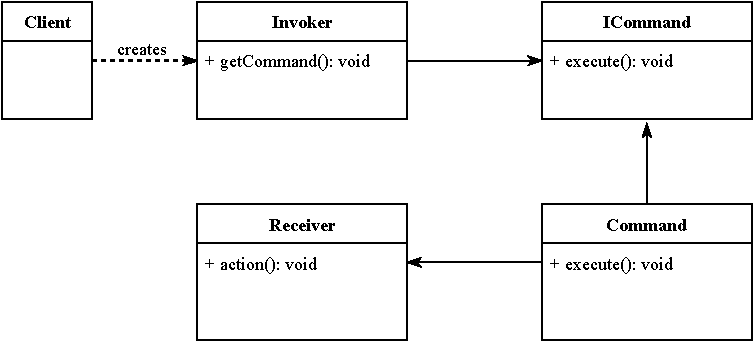
\includegraphics[width=1\textwidth]{fig/ainf/Command.pdf}
    \caption{UML-Diagramm Command}
    \label{fig:UML-Diagramm Command}
\end{figure}
\subsubsection{Beispiel}
\subsection{Entwurfsmuster MVC}\label{subsec:entwurfsmuster-mvc}
\subsubsection{Beschreibung}
Das MVC-Design Pattern, auch Model-View-Controller Design-Pattern, ist eines der weit verbreitetsten Entwurfsmuster.
Es dient zur Strukturierung von Anwendungen und teilt diese in 3 große Bereiche ab, welche strikt voneinander getrennt sind.
Mithilfe dieser Strukturierung fällt es dem Programmierer wesentlich leichter, spätere Änderungen bzw. Erweiterungen am Projekt durchzuführen, da das System nun klar definiert und strukturiert ist.
Auch ist es nun einfacher, parallel an dem Programm zu Arbeiten, denn Ersteller von View und Ersteller des Controllers, also der Berechnungen dahinter, sind nun nicht mehr voneinander abhängig.\\
Jedoch muss bedacht werden, dass Änderungen am Model, direkt an die View weitergegeben werden müssen.
\subsubsection{Struktur}

\begin{enumerate}
    \item \textbf{View}  \\
    Datenrepräsentation\\
    Organisiert alle Kontrollelemente
    \item \textbf{Controller} \\
    Stellt die Verbindung zwischen View und Model her\\
    Verwaltet Benutzerinteraktion und enthält Steuerlogik
    \item \textbf{Model} \\
    Datenrepräsentation\\
    Komplett Abgeschirmt
\end{enumerate}
\begin{figure}[H]
    \centering
    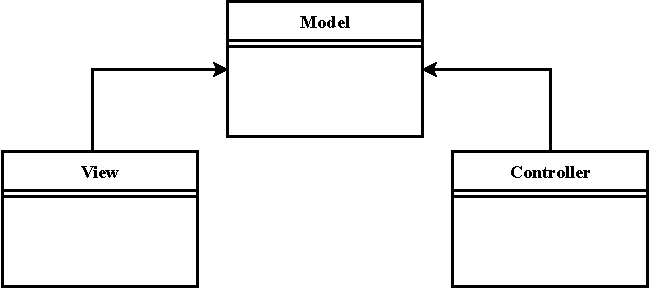
\includegraphics[width=0.8\textwidth]{fig/ainf/ModelViewController.pdf}
    \caption{UML-Diagramm MVC}
    \label{fig:UML-Diagramm MVC}
\end{figure}
\subsection{SceneBuilder}\label{subsec:scenebuilder}
\subsubsection{Beschreibung}
Scenebuilder ist ein umfangreiches GUI-Design-Tool der Firma Gluon.
Verwendet wird es bei Erstellung komplexerer Layouts, denn je komplizierter dieses wird, desto eher stößt man ohne Design-Tool an seine Grenzen.\\\\
Die Verwendung von Tools wie dieses hat mehrere Vorteile.
Einerseits Verbessert sich die Übersichtlichkeit des GUI-Projekts deutlich, da es ab diesem Zeit Zeitpunk möglich ist, den Code hinter der Oberfläche grafisch darzustellen.
Andererseits kann nun, nur mit wenigen Klicks eine für den Endbenutzer ansprechende GUI gebaut werden.\\
Im speziellen hat SceneBuilder weitere wichtige Vorteile wie die direkte Verbindung mit JavaFX und dessen \lstinline{*.fxml} Dateien.
Weiters ist es möglich CSS-Dateien sowie Internationalisierungsdateien einzubinden und diese direkt in SceneBuilder zu verfeinern.
Im wesentlichen ist SceneBuilder, gezeigt in der \autoref{fig:Tool SceneBuilder}, ein performantes Tool und eigent sich optimal für große Projekte wie dieses.
\begin{figure}[H]
    \centering
    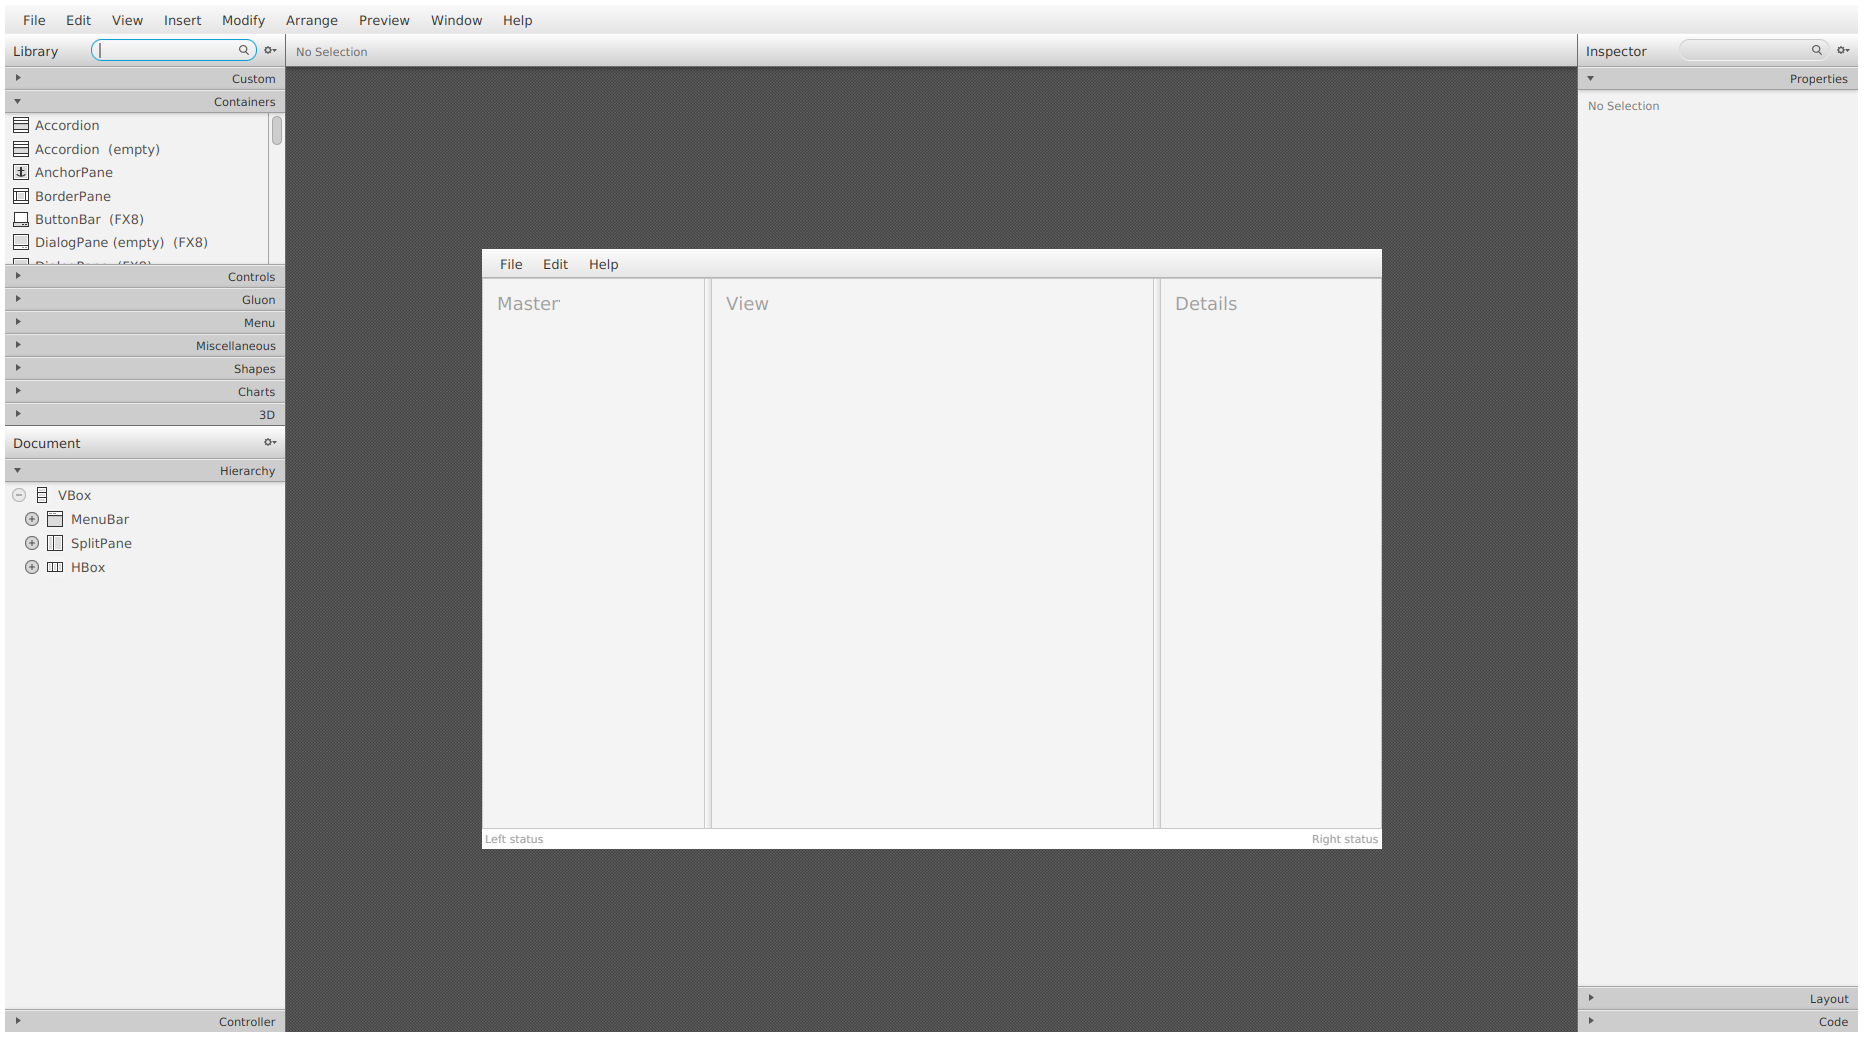
\includegraphics[width=0.8\textwidth]{fig/ainf/SceneBuilder.png}
    \caption{Tool SceneBuilder}
    \label{fig:Tool SceneBuilder}
\end{figure}
\subsubsection{Bibliothek JFoenix}
Sobald nun SceneBuilder als wichtiges Element der Erstellung ausgewählt wurde, kann jetzt ein näherer Blick auf die User-Experience geworfen werden.
Diese sogenannte User-Experience beschreibt, wie der Endbenutzer das Produkt bzw. in unserem Fall die grafische Oberfläche empfindet.
Wird auf diesen Kernpunkt kein Wert gelegt, wird auch niemand erfreut bei der Bedienung sein.\\\\
SceneBuilder bietet bereits einige Grundelemente für Layouts an, doch diese sind nicht ansprechend.
Sie können zwar mir CSS, was im \autoref{sssec: CSS} beschrieben wird, gestaltet werden, dies ist jedoch für alle Elemte schwierig umzusetzten.
Abhilfe schafft dabei die Material-Design Bibliothek von JFoenix.
Diese Bibliothek ist Open-Source und implementiert, wie schon im Namen genannt, Designelemente nach dem von Google entwickelten Material-Design Vorgaben.
Das bedeutet das ohne viel Aufwand, eine höchst ästhetische Oberfläche gebaut werden kann.
Zusätzlich kann man auch hier, eigene CSS-Deklarationen vornehmen, jedoch ist vieles schon vorab definiert\\
Anhand der folgenden \autoref{fig:Rendered Button} soll gezeigt werden, wie nun Elemente, gebaut mithilfe der JFoenix Bibliothek, aussehen.
Angewendet werden die Attribute \lstinline{-fx-border-radius: 20pt;}  \lstinline{-fx-background-radius: 20pt;} und \lstinline{-fx-background-color:grey}
\begin{figure}[H]
    \centering
    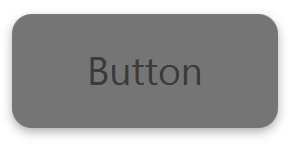
\includegraphics[width=0.4\textwidth]{fig/ainf/RenderedButton.PNG}
    \caption{Gerenderter Button}
    \label{fig:Rendered Button}
\end{figure}
\subsection{Datenformate in Java-FX}\label{subsec:datenformate-in-java-fx}
Im folgenden Kapitel soll auf die Datenpersistenz eingegangen werden.
Speziell in diesem Projekt werden die Datenformate \textbf{XML/FXML}, \textbf{CSS} und \textbf{JSON} verwendet.
Ziel ist es, grundlegende Dinge zu klären und einen kurzen Überblich zu erschaffen.
\subsubsection{XML}
XML(Extensible Markup Language) ist, wie im \autoref{sssec: JavaFX} schon erwähnt, eine Sprache zur Darstellung von Daten in einem von Menschen lesbaren Format.
Damit ist sie also keine Programmiersprache.
Diese XML-Dateien sind zu vergleichen mit normalen Textdokumenten, welche mit einen gewöhnlichen Texteditor geöffnet werden können.

Strukturiert und bezeichnet werden in XML-Dateien die Daten mithilfe von sogenennaten XML-Tags.
Diese Tags stehen in spitzen Klammern und beinhalten den Namen des Datenelements.
Auch ist es notwendig, ein Tag mihilfe eines sogenannten End-Tags zu schließen.
Zwischen diesen Start- bzw. \ End-Tags befindet sich ein Datensatz.
Ein Indikator für ein End-Tag ist ein \lstinline{/}.\\
Zwischen diesen Start- bzw. \ End-Tags befindet sich e
in Datensatz.
Ein Indikator für ein End-Tag ist ein \lstinline{/}.
Anhand der folgenden \autoref{xmlExample} soll gezeigt werden, wie XML-Dateien im inneren aussehen.
% @formatter:off
\begin{lstlisting}[style=XML,caption=XML-Codebeispiel,label=xmlExample]
<?xml version="1.0" encoding="UTF-8"?>
    <email>
        <to>Person1</to>
        <from>Person2</from>
        <heading>Test-Header</heading>
        <body>This is a body :)</body>
    </email>
\end{lstlisting}
% @formatter:on
\subsubsection{FXML}
FXML ist ein auf XML basierendes Datenformat, welches hauptsächlich bei der Erstellung von JavaFX Anwendungen angewendet wird.
Da die Trennung von GUI- und Programmcode bei Java FX nach dem MVC-Pattern \autoref{subsec:entwurfsmuster-mvc}vollzogen wurde, kann erst mithilfe des von Oracle entwickelte Formats ein Layout in einer eigenen Datei gebaut werden.\\\\
Die Struktur und Syntax von FXML Dateien ähnelt der von XML-Dateien.
So werden auch Start- und End-Tags verwendet.
Ein wesentlicher Unterschied ist jedoch bei der Groß-/Kleinschreibung ersichtlich.
Beginnen in FXML-Dateien Elemente mit einem Großbuchstaben, werden diese als Objektdeklarationen behandelt.
Infolgedessen erkennt der FXML-Loader, welcher diese \lstinline{*.fxml} ins Programm lädt, diese Objektdeklarationen nimmt eine dementsprechende Objektbildungen vor.
Sobald diese jedoch mit einem Kleibuchstaben beginnen, definieren sie Eigenschaften.
Eine weitere Besonderheit liegt bei dem Einbinden von Importanweisungen vor.
Dies können mithilfe des Tags \lstinline{<?import ... ?>} ausgeführt werden.\\
\begin{lstlisting}[style=XML,caption=FXML-Codebeispiel,label=fxmlExample]
<?xml version="1.0" encoding="UTF-8"?>
<?import javafx.scene.layout.VBox?>
<?import javafx.scene.control.Label?>

<VBox>
    <children>
    <Label text="Hello ReShuffled :)"/>
    </children>
</VBox>
\end{lstlisting}

\subsubsection{CSS}\label{sssec:CSS}
CSS ist eine Gestaltungs- und Formatierungssprache mit welcher Gestaltungsanweisungen erstellt werden können.
Es soll also beachtet werden, dass CSS nichts mit dem eigentlichen Inhalt der Website oder dem Programm zu tun hat, sondern rein für Design und Stilaspekte verwendet wird.\\
\footfullcite{JavaFXCSSReferenceGuide} Für unsere Anwendung bieten JavaFX Cascading Style Sheets (CSS) eine Möglichkeit, die Designziele aus dem \autoref{subsec:fronted-programmierung} umzusetzten und zu verfeinern.
Diese genannte Designsprache stellt eine Erweiterung vom standartisierten CSS mit einigen zusätzlichen Features dar.\\
Grundlegend besteht das Ziel von Java-FX CSS darin, Webprogrammierer, welche CSS bereits für Webanwendungen verwendet haben, die Möglicket zu geben, speziell für JavaFX zugeschnittene Themes zu bauen.
Diese Themes können auf die jeweiligen Kontrollelemente angewendet werden.\\
Eine Besonderheit von JavaFX CSS besteht im Vergleich zur normalen CSS-Sprache.
Alle Elemente, welche mit JavaFX in Verbindung stehen besitzen das Prefix \lstinline{-fx-...}.
Dies lässt sofort auf die Beschreibung eines JavaFX Elements schließen.
\subsection{Datenformat JSON}\label{subsec:json}

\subsubsection{Beschreibung}
Der Name JSON(JavaScript Object Notation) beschreibt neben XML eines der wichtigsten Datenformate zur Sicherstellung der Datenpersistent in der Softwaregeschichte.
Dieser Nachfolger von CSV und INI setzte sich vorallem in der heutigen Datentechnik durch.
Grundlegend ist JSON wiederum ein textuelles Datenformat, welches kompakt und einfach lesbar ist.
Ein weiterer Grund zur Verwendung ist ebenso eine effektive Umwandlung von Daten, also Objekten, Arrays und sonstigen Variablen,  in das JSON-Dateiformat.\\
All diese Merkale sind esentiell wichtig und eröffnen ein breites Spektrum an Verwendungsmöglichkeiten.\\\\
Die Syntax von JSON ist klar definiert und wird ebenfals durch ein Beispiel näher visualisiert.
\begin{lstlisting}[style=json, caption=JSON-Codebeispiel,label=jsonExample]
{
    "employee": {
    "name": "tester",
    "salary": 5432,
    "children": false
    }
}
\end{lstlisting}
\subsubsection{Bibliothek Gson}\label{sssec:gson}
Die von Google entwickelte Bibliothek Gson spielt in diesem Projekt eine wichtige Rolle.
Aufgrund enormer Datenmengen ist es zeitaufwändig, JSON Dateien in Java zu erstellen.\\
Eine Hilfe bietet dabei Gson.
Diese unterstützende Bibliothek hilft dem Emtwickler bei der Konvertierung zwischen Java-und JSON-Objekten.
Erstellt wird eine Gson Instanz durch Aufruf des Default-Konstruktors: \lstinline[style=java]{Gson gson = new Gson()}.
Sobald dies vonstatten gegangen ist kann nun entweder mit der Methode \lstinline{toJson} oder mit \lstinline{fromJson} gearbeitet werden.
Diese beiden Methoden stellen die Haupteinstiegspunkte von Gson dar und werden im folgenden Teil erklärt.
\\\\
\textbf{\lstinline{toJson}}
\\
Mithilfe der Mehode \lstinline[style=java]{gson.toJson()} kann direkt aus einem Objekt ein JSON-String erzeugt werden.
Dieser genannte String kann danach je nach belieben in eine Datei geschreiben oder versendet werden.
\\\\
\textbf{\lstinline{fromJson}}
\\
Auch kann der gesamte Prozess mithilfe des Methodenaufrufs \lstinline[style=java]{gson.fromJson()} umgekehr werden.
Hierbei wird aus einem JSON-String ein Objekt erzeugt.
\\
\section{Backend-Programmierung}\label{sec:backend-programmierung}
\subsection{Kommunikation}
\subsubsection{Konzept}
Um erfolgreich Daten zwischen dem Raspberry PI 3B+ und der Platine, welche die Ansteuerung sämtlicher Komponenten übernimmt, zu übertragen, wird ein Kommunikationsprotokoll benötigt.
Dieses Protokoll stellt im engsten Sinne eine Vereinbarung dar, wie die Datenübertragung zwischen zwei oder mehreren Parteien abläuft.
Anforderungen an dieses Protokoll sollen sein:
\begin{enumerate}
    \item einfache Integration in die Zielsysteme
    \item erweiterbarkeit des Protokolls mit geringem Arbeitsaufwand
    \item hohe Sicherheit gegenüber Übertragungsfehler
    \item schnelle Fehlererkennung sowie Fehlerbehebung
\end{enumerate}
Neben standartisierten Protokollen wie Modbus, Feldbus oder CAN-Bus gibt es die Möglichkeit selbst ein sogenanntes propretäres Übertragungsprotokoll zu kreieren.
Dies ist in unserem Fall nötig, um alle Anforderungen abzudecken.
Basierend auf dem Master - Slave Prinzip, wobei der Rasperry PI den Master und die Ansteuerplatine den Slave darstellt, soll ein abgewandeltes Modbus ASCII Protokoll umgesetzt werden.

Zusätzlich soll, um die Anforderung des einfachen Fehlerhandlings zu erfüllen, ein Simulator ausprogrammiert werden, welcher beim Start auf Softwarebebene, den Platz des Slaves bzw. der Ansteuerplatine einnimmt.
Der Startvorgang des Simulators soll mit einer einfachen Modifizierung der Konfigurationsdatei vonstatten gehen.
Die folgende Grafik soll die schematisch die Geräteauswahl darstellen.
\begin{figure}[H]
    \centering
    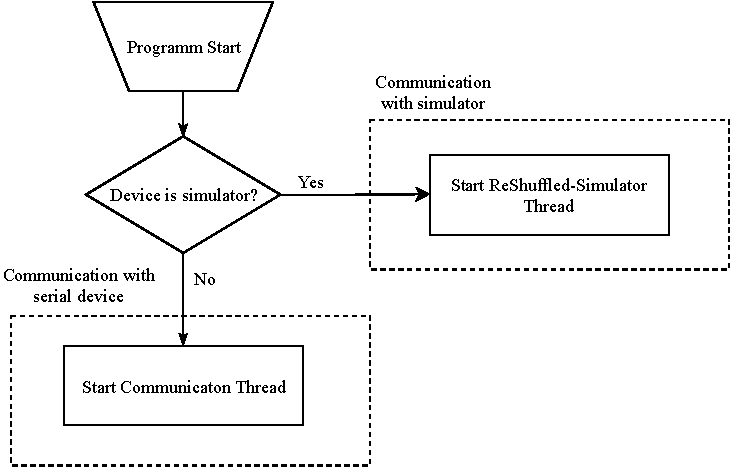
\includegraphics[width=0.6\textwidth]{fig/ainf/DeviceSelection}
    \caption{Schematische Darstellung der Geräteauswahl}
    \label{deviceSelection}
\end{figure}
\subsubsection{Übertragungsprotokoll} \label{sssec:uebertragungsprotokoll}
\begin{table}[H]
    \centering
\resizebox{\textwidth}{!}{%
    \begin{tabular}{|
    >{\columncolor[HTML]{FFFFFF}}l |
    >{\columncolor[HTML]{FFFFFF}}l |
    >{\columncolor[HTML]{FFFFFF}}l |
    >{\columncolor[HTML]{FFFFFF}}l |
    >{\columncolor[HTML]{FFFFFF}}l |}
        \hline
        \textbf{Doppelpunkt :} & \textbf{Daten (ASCII)} & \textbf{Trennzeichen \#} & \textbf{CRC32-Prüfsumme} & \textbf{Semicolon \textbackslash{}n} \\ \hline
        8-Bit & 16-Bit & 8-Bit & 32-Bit & 8-Bit                                \\ \hline
    \end{tabular}
}
    \caption{Visualisierung des Datenakets}
\end{table}
Das verbindugslose Protokoll basiert, wie in der Konzeptbeschreibung bereits erwähnt, auf dem Master-Slave Prinzip.
Außerdem erfolgt die Datenübertragung rein textuell wobei nur Großbuchstaben verwendet werden dürfen.\\\\
Wie aus der oben dargestellten Tabelle zu entnehmen, ist der Aufbau eines Frames klar definiert.
Der eindeutige Start des Datenpakets, welcher mit einem Doppelpunkt (:) eingeleitet wird, sowie das ebenfalls eindeutige Ende, umgesetzt mit einem Line Feed Character (), bringt eindeutige Vorteile mit sich.
Im Gegensatz zu anderen Protokollen wie z.B. Modbus RTU, muss hier nicht auf das Ende des Pakets "gewartet" werden.
Dies führ oft zu Einbußen im Bereich der Performance und ist für uns nicht zielführend.\\\\
Gefolgt von dem Startzeichen folgen nun die Daten.
Diese beinhalten eindeutig definierte Zecichenfolgen, welche verwendet werden um verschiedenste Zustände der Ansteuerplatine auszuführen.
Diese Um auch hier zu wissen, wo sich das der Nutzdaten befindet, schließt das Trennzeichen () diese ab.\\\\
Um nun die Integrität, also die Korrektheit der Daten bei einer Übertragung zu überprüfen, wird im nächsten Schritt eine Prüfsumme verwendet.
Ziel dieser ist es, anhand der Nutzdaten einen Wert zu bilden, welcher danach vom Sender im Frame gespeichert bzw übertragen wird.
Der Empfänger berechnet nun mit dem selben Verfahren die Prüfsumme aus den empfangenen Daten und vergleicht diese mit der Übertragenen Prüfsumme des Senders.
Sind beide Prüfsummen identisch, war die Übertragung erfolgreich und die Daten sind mit großer Wahrscheinlichkeit korrekt.
Stimmen diese nicht überein liegt ein Fehler vor.
Die wichtigsten Arten von Übertragungsfehlern sind:
\begin{enumerate}
    \item Einzelbitfehler (1 Bit verändert)
    \item Burstfehler (ganze Folge von Bits verändert)
\end{enumerate}
Neben einfachen Verfahren wie z.B. dem Paritätsbit-Verfahren gibt es auch Komplexere.
Die zyklische Redundanzprüfung, auch CRC genannt, ist eines davon.
Sie ist realtiv einfach zu realisieren und dennoch wirkungsvoll.
Wichtig beim CRC-Verfahren ist, dass beide Teilnehmen, also Sender und Empfänger, das selbe Generator-Polynom verwenden.
Der Grad des Generatorpolyoms beträgt in unserem Fall 32 (CRC-32).
\subsubsection{Request- und Responsebeispiele}
Folgend wird anhand von tabelarisch aufgelisteten Beispielen gezeigt, wie ein Request mit dem jeweiligen Response zusammenhängt.
Jeder Request sowie Reponse basiert auf der Protokolldefinition aus dem \autoref{sssec:uebertragungsprotokoll}.
\begin{table}[H]
\centering
\resizebox{\textwidth}{!}{%
\begin{tabular}{|l|l|l|c|}
\hline
\rowcolor[HTML]{FFFFFF}
\textbf{Request} & \textbf{Request-String {[}Rx{]}} & \textbf{Aktion} & \multicolumn{1}{l|}{\cellcolor[HTML]{FFFFFF}\textbf{Response-String {[}Tx{]}}} \\ \hline
Init     & IN                                          & Initialisierungs-Zustand     & \multicolumn{1}{l|}{OK oder E\textless{}Code\textgreater{}} \\ \hline
Shutdown & XX                                          & Herunterfahren der Maschine  & --//--                                                      \\ \hline
Shuffle  & SH                                          & Mischen von Karten           & --//--                                                      \\ \hline
Deal     & D\textless{}Anzahl der Karten\textgreater{} & Kartenausgabe je nach Anzahl & --//--                                                      \\ \hline
AutoDeal & A\textless{}Anzahl der Karten\textgreater{} & Automatische Kartenausgabe   & --//--                                                      \\ \hline
\end{tabular}%
}
\caption{Request- und Responsebeispiele Tabellarisch dargestellt}
\end{table}
Aufgrund eines wohldurchdachten Systems bei der Request-Definition, ist es nun möglich, den Pool an verschiedenen Requests explizit zu minimieren.
Dies bezieht sich auf den Vorgang der automatischen Kartenverteilung an jeden den einzelnen Spieler, was mithilfe des Requests \textbf{Deal} und \textbf{AutoDeal} umgesetzt wird.\\
Neben den Request, welche sich rein auf den Ablauf eines Kartenspiels konzentrieren, verfügt der Pool über Requests, welche allgemein zur Funktionalität der Maschine beitragen.
Der Request \textbf{Shutdown} führt jedeglich zu einem Herunterfahren der Maschine.
Auch wird bevor die Maschine in Betrieb genommen wird, der Request \textbf{Init} gesendet.
Dieser hat den Sinn und Zweck, die Maschine in einen Initialisierungszustand zu versetzten.\\
Die genauere Aufarbeitung und Umsetztung sei im \autoref{ssec:konzeptCardDeal} verzeichnet.
\subsubsection{Umsetztung-Datenaustausch}
Zuallererst soll der Ablauf der Kommunikation zwsichen dem Programm und dem Endgeräts, welches über die serielle Schnitstelle verbunden ist, betrachtet werden.
Im ersten Schritt wird auf die Erstellung jedes einzelnen Request eingegangen.\\
Um die Aufgabe der Einbindung von Requests elegant und objektorientiert umzusetzten, stellt die abstrakte Klasse \lstinline[style=java]{Request} den Kopf jedes einzelnen Requests dar.
Dies bedeutet im engsten Sinne, dass jeder einzelne Request eine Abstammung dieser Klasse ist.
Dargestellt wird dies auch durch das generierte UML-Diagramm in \autoref{umlReq}
\begin{figure}[H]
\centering
\vspace{-5mm}
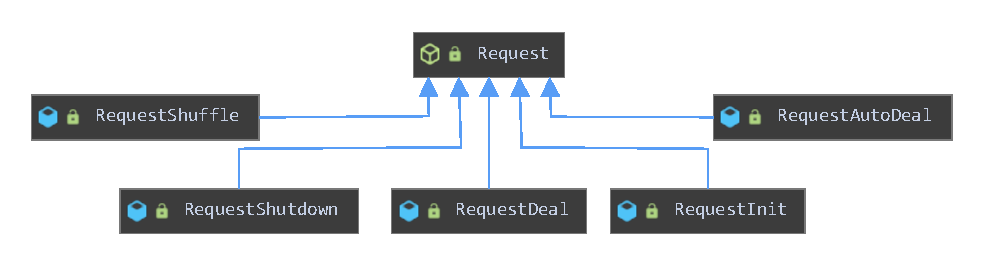
\includegraphics[width=1\textwidth]{fig/ainf/RequestUML.pdf}
\caption{UML-Diagramm-Request-Baum}
\label{umlReq}
\end{figure}
Bevor nun auf jeden einzelnen Request eingegangen wird, soll nun die abstrakte Klasse \lstinline[style=java]{Request} betrachtet werden.
Diese Klasse implementiert die Methoden \lstinline[style=java]{createRequestFrame()}, \lstinline[style=java]{handleRequestSent()} und \lstinline[style=java]{handleResponse()}.\\\\
Wie der Namen der Methoden schon ahnen lässt, ist \lstinline[style=java]{createRequestFrame()} für die Erstellung jedes Request zuständig.
Diese Methode hat hat ist \lstinline[style=java]{protected} somit kann von den abstammenden Requests darauf zugegriffen werden.
\lstinputlisting[firstline=90, lastline=102, style=java,caption=fdsa,label=Gesamte Methode createRequestFrame()]{src/serial/request/Request.java}
Sobald die Methode von einem abstammenden Request aufgerufen wird und der Content, also der Request-String, übergeben wird, überprüft diese Mathode den übergebenen Content.
Sollte dieser leer leet sein wird eine \lstinline[style=java]{IllegalArgumentException} geworfen und die Erstellung des Requests wird somit abgebrochen.
Ist jedoch ein Content vorhanden wird mithilfe der Bibliothek \lstinline{CRC32} eine CRC-32 Prüfsumme erzeugt und in ein hexadezimales Format geparst.
Letztendlich wird danach der Request-String mithilfe eines \lstinline{StringBuilders} zusammengebaut.
Das für die Datenspeicherung im Objekt zuständige Atrribut benennt sich \lstinline[style=java]{private byte[] resFrame} und speichert dessen Daten in ein Byte-Array.\\\\
Weiters verfügt die Klasse die Methode \lstinline[style=java]{handleRequestSent()} welche ausschließlich die Aufgabe hat, den definierten Zeitstempel \lstinline[style=java]{timeMillisFrameSent} zu setzten.
Dieser genannte Zeitstempel ist im nachhinein für das Timeout-Handling von Responses wichtig.\\
Sobald nun ein Response ankommt, kommt die Methode \lstinline[style=java]{handleResponse()} ins Spiel.
Aufgabe dieser ist es, das akommende Response-Objekt, welches im unteren Abschnitt beschreiben wird, in dessen elementaren Daten zu zerlegen.
\lstinputlisting[firstline=35, lastline=42, style=java,caption=fdsa,label=handleResponse() Teilabschnitt]{src/serial/request/Request.java}
Auch soll wiederum in dieser Methode überprüft werden, ob der Content des Frames Fehler aufweist. Dies geschieht wieder mithilfe der in Java implementierten Bibliothek \lstinline{CRC32} und soll nicht näher beleuchtet werden.
Nun wird anhand des zurückkommenden Response-Strings analysiert, wie sich der Request im Zielsystem verhalten hat.
Wie im Protokoll definiert kann nun entweder ein \lstinline[style=java]{OK} oder ein Errorcode mit dem Prefix \lstinline[style=java]{E} zurückkommen.
Der Pool an Codes kann jedoch nur ein Volumen von 9 annehmen, da ansonsten der Frame zu groß wäre.
Umgesetzt wird die Analyse mithilfe einer switch-case-Verzweigung.
\lstinputlisting[firstline=61, lastline=86, style=java,caption=fdsa,label=handleResponse() Teilabschnitt]{src/serial/request/Request.java}
Jeder einzelne Error steht für eine spezielle Fehlerquelle bei der Ausführung.
Eine Übersicht wird in \autoref{ssec:konzeptCardDeal} gegeben.\\\\
Zusätzlich wird in der Klasse \lstinline[style=java]{Request} die \lstinline[style=java]{toString()} Methode überlagert.
Dadurch kann das Request Objekt nun optimal in einen String umgweandelt werden.
Nun betrachten wir die spezifischen Request, welche in \autoref{umlReq} zu sehen sind.\\
Im Prinzip ist der Aufbau jeder Request Klasse ähnlich.
Aufgerufen wird der Konstruktor welcher die Methode \lstinline[style=java]{createRequestFrame()} ausführt.
Als Parameter erhält diese Methode den vom Protokoll festgelegten Content.
Als Beispiel soll der Request Shuffle gezeigt werden.
\lstinputlisting[firstline=8, lastline=12, style=java,caption=fdsa,label=toString() Methode]{src/serial/request/RequestShuffle.java}
\textbf{Conclusion:}\\
Somit erhält man nach Erstellung eines Objekts vom gewählten Request-Typ ein vollwärtiges Onjekt mit dem gearbeitet werden kann.
Im folgenden Abschnitt wird nun gezeigt, wie ein Request versendet werden kann.\\\\
Die gesamte Kommunikation wird umgesetzt durch die Klasse \lstinline[style=java]{Communication}.
Diese kann verglichen werden mit einem Wächter, welcher sich um das Senden und Empfangen von Daten kümmert.
Die vom Designpattern Singelton abgeleitete Klasse stellt 2 Threads bereit, wobei einer davon für den Sendung- und einer für den Empfangsvorgang zuständig ist.
Beide werden im privaten Konstruktor der Klasse erstellt und gestartet.
Somit ist ab diesem Zeitpunkt die Verfügbarkeit zur Kommunikation gegeben.\\\\
\textbf{Der CommunicationSendThread:}\\
Nun besteht jedoch das Problem, das  untereinander abgestimmt werden müssen.
Ein wichtiges Beispiel zeigt hierbei das \textbf{Producer-Consumer-Problem} welches in der \autoref{ProducerConsumer} dargestellt wird.
\begin{figure}[H]
\centering
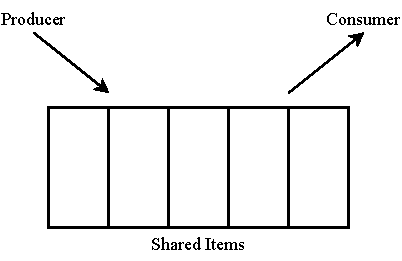
\includegraphics[width=0.45\textwidth]{fig/ainf/ProducerConsumer.pdf}
\caption{Kommunikation Producer-Consumer}
\label{ProducerConsumer}
\end{figure}
Dies bezieht sich auf die gemeinsame Verwendung von Items, da hier Überschneidungen entstehen.
In diesem Fall stellet die sogenannte \lstinline[style=java]{toSentList}, welche als LinkedList vom Typ \lstinline[style=java]{Request} implementiert wurde, die Items dar.
Einerseits müssen hier Requests zur Liste hinzugefügt und andererseits entnommen werden.\\
Um nun die Thread-Sicherheit zu gewährleisten und Deadlocks zu vermeiden, wurde von \lstinline[style=java]{synchronized()} gebrauch gemacht.
Wie schon im oberern Teil beschrieben, bietet die sogenannte \lstinline[style=java]{toSentList} eine gemeinsame Ablage von Requests.
Bei jedem Zugriff wird nun also mit \lstinline[style=java]{synchronized(toSentList)} gearbeitet.
Mithilfe der Methoden \lstinline[style=java]{wait()} und \lstinline[style=java]{notify()} wurde nun eine Möglichkeit geschaffen, um Busy-Waiting, zu vermeiden.
Hier wartet bzw "schläft" der Thread, bis er von außen aktiviert also "aufgeweckt" wird.
Zu sehen ist dies im \autoref{commThreadSync}.
% @formatter:off
\begin{lstlisting}[style=java,caption=Java-Codebeispiel,label=commThreadSync]
try {
    mainLoop:
    while (!Thread.currentThread().isInterrupted()) {
        synchronized (toSentList) {
            LOG.fine("Thread waiting for items ...");
            toSentList.wait();

            if (!toSentList.isEmpty()) {
            ....
            }
        }
    }
}
catch (Exception ex) {
    LOG.warning(ex, Thread.currentThread().getName() + " exception");
}
finally {
    LOG.info(Thread.currentThread().getName() + " ended");
}
\end{lstlisting}
% @formatter:on
Hinzugefügt kann ein Item über die Methode \lstinline[style=java]{public void sendRequestExecutor (Request req)} werden.
Diese Methode, welche nach dem Command-Verhalensmuster (\autoref{subsec:verhaltensmuster-command}) gestaltet wurde, fügt ledeglich ein Element zur Liste hinzu und "weckt" den Thread mit \lstinline[style=java]{notifyAll()}.
\lstinputlisting[firstline=61, lastline=67, style=java,caption=fdsa,label=toString() Methode]{src/serial/Communication.java}
Befindet sich nun etwas in der \lstinline[style=java]{toSentList}, beginnt der Thread zu arbeiten.
Ein Loop zur Sendung eines Request kann einfach anhand des \autoref{commThreadSend} erklärt werden.
% @formatter:off
\begin{lstlisting}[style=java,caption=Java-Codebeispiel,label=commThreadSend]
if (!toSentList.isEmpty()) {
    pendingRequest = toSentList.removeFirst();
    LOG.fine("sending request " + pendingRequest.getMreqFrame());
    serial.writeString(pendingRequest.getMreqFrame());
    pendingRequest.handleRequestSent();
}
\end{lstlisting}
% @formatter:on
Vorerst wird der wartende Request in dem Attribut \lstinline[style=java]{Request pendingRequest} gespeichert und von der Liste gelöscht.
Danach kann dieser über die serielle Schnitstelle versendet werden.
Dies erfolgt mithilfe der Hilfsmethode \lstinline[style=java]{serial.writeString()} welche im \autoref{sssec:deviceSelection} beschrieben wurde.\\\\
Nun soll auf den ankommenden Response gewartet werden.
Auch hier wird eine LinkedList implementiert.
Diese besteht jedoch nicht aus Request-Objekten, sondern aus sogenannten Response-Objekten.
In jedem einzelnen Objekt vom Typ \lstinline[style=java]{Response} befindet sich der Frame, gepeichert in dem Attribut \lstinline[style=java]{byte [] resFrame}, und ein Zeitstempel namens \lstinline[style=java]{long timeMillisCreatedAt}.\\\\
Wird nun vom CommunicationReceiveThread, welcher später beschrieben wird, empfangen und zur \lstinline[style=java]{responseList} hinzugefügt, entfernen die folgenden Zeilen Code den Request von der Liste und speichern diesen.
% @formatter:off
\begin{lstlisting}[style=java,caption=Java-Codebeispiel,label=commThreadSend]
res = responseList.removeFirst();
if (!responseList.isEmpty()) {
    LOG.warning("response list should be empty, but " + responseList.size() + " items in list");
    responseList.clear();
}
\end{lstlisting}
% @formatter:on
Mithilfe des Methodenaufrufs \lstinline[style=java]{pendingRequest.handleResponse(res)} wird nun, wie oben beschreiben, der Response weiter verarbeitet.\\\\
Sollte jedoch kein Response ankommen, versucht das Programm, sofern in der Konfigurationsdatei ein zweiter Versuch erlaubt ist, den selben Response nochmals zu senden.
Ist dies nicht der Fall, wird eine \lstinline[style=java]{SerialException} geworfen.
% @formatter:off
\begin{lstlisting}[style=java,caption=Java-Codebeispiel,label=commThreadSend]
if (responseList.isEmpty()) {
    if (Config.getInstance().getConfigSerial().isSecondTryAllowed()) {
        sendRequestExecutor(pendingRequest);//send second response
        continue mainLoop;
    }
throw new SerialException("request timeout, mssing response"); // if second try isnt allowed throw serial exception
}
\end{lstlisting}
% @formatter:on
Somit wäre ein Kommunikations-Loop abgeschlossen und der CommunicationSendThread wartet wieder auf ankommende Requests des Programms.\\\\
\textbf{Der CommunicationReceiveThread:}\\
Nun sollte jedoch das Empfangen eines Response näher beschrieben werden.
Dieser sogenante CommunicationReceiveThread holt sich vorerst den InputStream und liest danach die Zeichen ein.
Ist das ankommende Zeichen ein \lstinline[style=java]{:}, beginnt er, die folgenden Zeichen einschließlich des \lstinline[style=java]{:} in einen Buffer zu speichern.
Sollte jedoch ein unerwartetes Zeichen ankommen, was oft auf einen Übertragungsfehler hinweist, wird ein Eintrag in die Log-Datei erstellt, welcher den Fehler veranschaulicht.
% @formatter:off
\begin{lstlisting}[style=java,caption=Java-Codebeispiel,label=commThreadSend]
while (!Thread.currentThread().isInterrupted()) {
    int b = is.read();
    if (b >= 0 && b < 255) {
        if (bufferIndex == 0) {
            if (b == ':') {
                buffer[bufferIndex++] = (byte) b;
            }
        else {
            LOG.warning("receiving unexpected byte (':' expected, get " + b);
        }
        }
\end{lstlisting}
% @formatter:on
Werden die ankommenden Daten nun als vollwärtigen Request empfunden, fügt der CommunicationReceiveThread diesen zur oben genannten \lstinline[style=java]{responseList} hinzu und weckt den CommunicationSendThread, welcher diesen, wie oben beschreiben, weiterverarbeitet.
% @formatter:off
\begin{lstlisting}[style=java,caption=Java-Codebeispiel,label=commThreadSend]
        else if (bufferIndex < buffer.length) {
            buffer[bufferIndex++] = (byte) b;
            if (b == '\n') {
                synchronized (responseList) {
                    byte[] resBuffer = Arrays.copyOf(buffer, bufferIndex);
                    bufferIndex = 0;
                    responseList.add(new Response(resBuffer));
                    responseList.notifyAll();
                }
            }
}
else {
LOG.warning("receiving byte " + b + " cannot be stored (receive buffer overflow)");
}
}
}
\end{lstlisting}
% @formatter:on
\subsubsection{Geräteauswahl} \label{sssec:deviceSelection}
%Nachdem nun ausführlich über den Serial-Simulator gesprochen wurde, wird nun im Folgenden die Geräteauswahl beschrieben.\\
Wie in der \autoref{deviceSelection} gezeigt, erfolgt die Auswahl der Gerätes, mit welchem kommuniziert wird, bei jedem Start-Vorgang.
Hierbei wird zuallererst die Konfigurationsdatei untersucht.
Ist hier der Eintrag \lstinline[style=json]{"device": "sim"} vorhanden, wird der Simulator gestartet und alle notwendigen Konfigurationen werden vorgenommen.
Sollte jedoch etwas anderes eingetragen sein, wird versucht auf serieller Ebene mit dem Gerät zu kommunizieren.
Ist dies der Fall, muss auch die serielle Schnittstelle vor der Verwendung konfiguriert werden.\\
All diese Aufgaben übernimmt die vom Designpattern-Singelton abgeleitete Klasse \lstinline[style=java]{Serial} und wird im folgenden Abschnitt beschrieben.\\\\
Wird im ersten Schritt eine Instanz der Klasse Serial mithilfe der Methode \lstinline[style=java]{createInstance()} erstellt, wird der private Konstruktor aufgerufen.
Dieser hat 2 wesentliche Aufgaben.\\
Einerseits soll er sicherstellen, dass sich alle Parameter der seriellen Schnittstelle in der Konfigurationsdateien befinden.
Umgesetzt wird dies mithilfe der Abfrage \lstinline[style=java]{if (config.isDisabled())}
Diese Parameter werden im Folgenden aufgelistet.
% @formatter:off
\begin{lstlisting}[style=json,caption=json-Codebeispiel,label=jsonSerial]
"serial": {
"disabled": false,
    "device": "sim",
    "baudrate": 57600,
    "timeoutMillis": 1000,
    "secondTryAllowed": false,
    "responseByteLength": 32
},
\end{lstlisting}
% @formatter:on
Ansererseits soll die Geräteauswahl mithilfe eines Abgleichs des Gerätenamens erfolgen.
Wird die Zeichenkette \lstinline[style=json]{"sim"} mithilfe der Abfrage \lstinline[style=java]{if (config.getDevice().equals("sim"))} erkannt, wird die Methode \lstinline[style=java]{initSimulation()} ausgeführt, ansonsten \lstinline[style=java]{initSerialDevice()}.
In diesen beiden Methoden werden sowohl die serielle Schnitstelle, als auch der Simulator konfiguriert.
% @formatter:off
\begin{lstlisting}[style=java,caption=Java-Codebeispiel,label=commThreadSend]
private Serial(ConfigSerialModel config) throws SerialException, IOException {
    this.config = config;

    if (config.isDisabled()) {
        return;
    }
    if (config.getDevice().equals("sim")) {
        initSimulation();
    } else {
        initSerialDevice();
    }
}
\end{lstlisting}
% @formatter:on
Nun soll anhand der Listings näher auf den Code der beiden Methoden eingegangen werden.
\\\\
\textbf{\lstinline{initSimulation()}}
\\
Vorerst soll angenommen werden, dass als Gerät der Simulator ausgewählt wurde.
Ist dies der Fall wird innerhalb der Methode \lstinline{initSimulation()} eine Möglichkeit zu Kommunikation mit dem Simulator geschaffen.
Realisiert wird diese Verbindung, wie im anschließenden \autoref{serialSim} beschrieben, mithilfe von Input- und Outputstreams.
Also werden diese zu Beginn definiert.\\
Um nun den Serial-Simulator zu starten ist ledeglich eine Erstellung des ReshuffledMainboardSimulator-Objekts notwendig.
Dieser erhält dessen Input- und Outputstreams übergeben von denen er aus kommuniziert.\\\\
So ist nun die volle Funktionalität des Simulators gegeben und es kann ohne "echte" Peripherie gearbeitet werden.
\lstinputlisting[firstline=69, lastline=87, style=java,caption=fdsa,label=fdsafdsa]{src/serial/Serial.java}
\textbf{\lstinline{initSerialDevice()}}
\\
Wird nun angenommen, dass es sich bei dem Konfigurationseintrag nicht um die Zeichenkette \lstinline[style=json]{"sim"} handelt, springt das Programm in die Methode \lstinline{initSerialDevice()}.
Erfolgt nun das Einlesen der im \autoref{jsonSerial} gezeigten Parameter, wird der Port zum Endgerät geöffnet.
Verwendet wurde hierbei die Open-Source-Bibliothek jSSC (Java Simple Serial Connector).
Erstellt wird eine Instanz des \lstinline[style=java]{jssc.SerialPort} mithilfe einer Objekterzeugung.
Diese forderdert als Parameter den Portnamen.
Nun kann mithilfe der Methode \lstinline{openPort()} der Port geöffnet werden.\\\\
Dieses genannte "Öffnen" des Ports kann unter gewissen Umständen zu einer \lstinline[style=java]{SerialPortException} führen.
Diese Umstände können vielseitige Ursachen haben und werden in der Javadoc von jSSC näher beschrieben.
Im darauffolgenden Schritt muss nun der Port mithilfe von \lstinline[style=java]{setParams()} konfiguriert und die Input- und Outputstreams für das serielle Endgerät definiert werden.\\\\
\lstinputlisting[firstline=89, lastline=103, style=java,caption=fdsa,label=fdsafdsa]{src/serial/Serial.java}
Ab diesem Zeipunkt wird das richtige Endgerät ausgewählt und es kann über den jeweiligen Stream kommuniziert werden.
Dies kann über die implementierte Methode \lstinline[style=java]{writeString()} geschehen, welcher direkt einen String als Parameter übergeben wird.
\lstinputlisting[firstline=105, lastline=109, style=java,caption=fdsa,label=fdsa]{src/serial/Serial.java}
Auf die Weiterverarbeitung der Daten an dem \lstinline[style=java]{SerialJsscInputStream} und \lstinline[style=java]{SerialJsscOutputStream} soll nicht weiter eingegangen werden, denn aufgrund der einfachen Implementierung ist dies selbstverstänglich und würde zur überladung des Kapitels führen.
Wiederum wird jedoch anschließend auf die Verarbeitung von Daten an den Simulator gesprochen, denn dies spielt eine wichtige Rolle und sollte nicht unerwähnt bleiben.
\subsubsection{Serial-Simulator}\label{sssec:serialSim}
\begin{figure}[H]
\centering
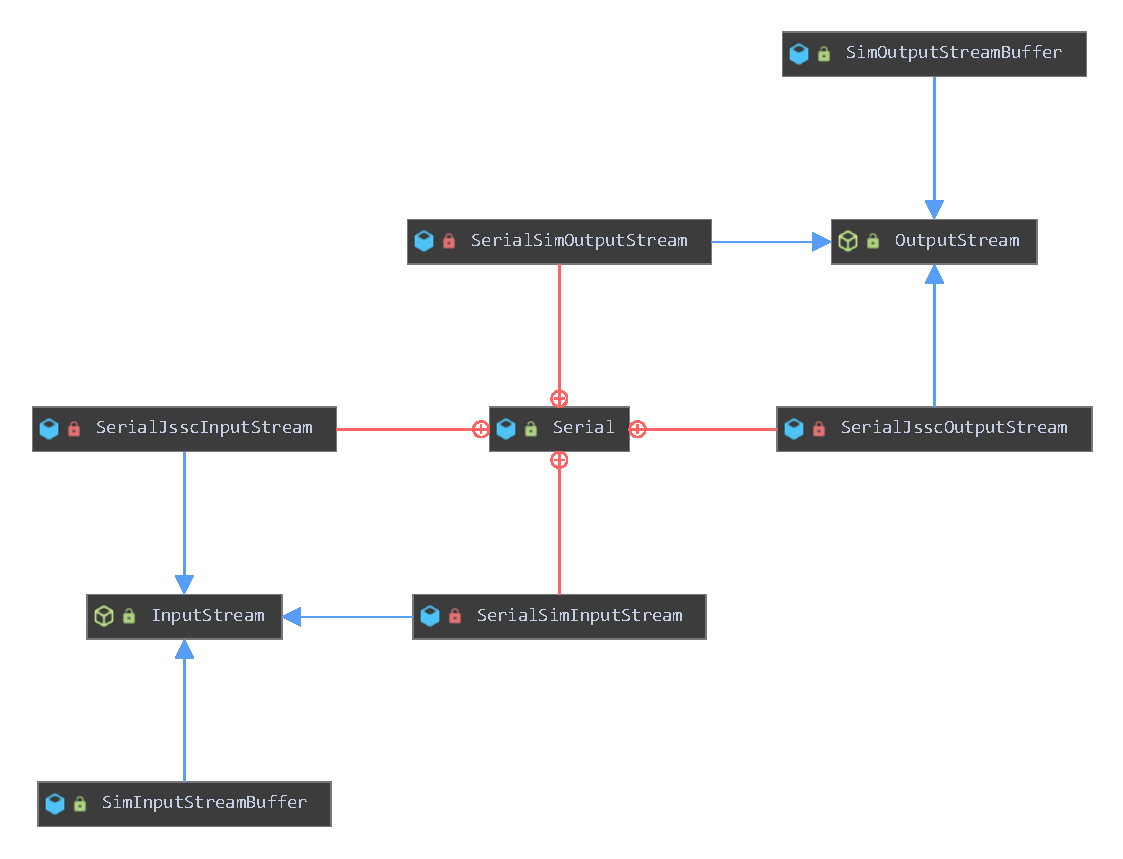
\includegraphics[width=0.9\textwidth]{fig/ainf/InputOutputStreams.pdf}
\caption{UML-Diagramm Streams}
\label{ProducerConsumer}
\end{figure}
\subsection{Logging}
\subsubsection{Konzept}\label{sssec:logOverview}
Logging ist nach dem Debugging selbst, dass zweitwichtigeste Mittel um einzelne Programmbausteine oder das gsamte Programm auf Fehler zu untersuchen.
Mithilfe einer Log-Datei können z.b aktuelle Wertebelegungen im Detail dargestellt werden.
Natürlich kann dies auch mithilfe einer Konsolenausgabe über \lstinline[style=java]{System.out.println()} realisiert werden, jedoch ist eine Verwendung von Logging-Frameworks immer sinvoller.\\\\
\textbf{Gründe für die Verwendung von Logging-Frameworks}\\
Als Beispiel kann mithilfe einer Log-Datei auch ein Benutzer, welcher nicht über die Möglichkeit verfügt, den Quellcode einzusehen, einzelne Fehler erkennen(vorrausgesetzt diese Möglichkeit ist durch das Programm geschaffen).
Auch ist nun die Persistenz der Logging-Einträge gegeben.
Dies bedeuted, es kann nun sichergestellt werden, dass diese Einträge auf dem System gespeichert werden und nach einem Neustart verfügbar sind.
Nutzt man diese Art von Protokollierung kann man außerdem die Genauigkeit der Erfassung genau parametrisieren.\\
Zusammengefasst bringt das Erstellen einer Log-Datei mithilfe eines Logging-Frameworks ein großes Feld an Möglichkeiten mit sich.\\\\
\subsubsection{Integration in das Programm}
Aufgrund der gegebenen Klassen, welche das Logging implementieren, ist die Integration in das Programm einfach umzusetzen.
Es ist ledeglich notwendig, diese genannten Klassen in ein unterpackage des Programms einzufügen.
Dazu soll in der \autoref{PackagestrukturLogging} die Struktur des Logging-Packages illustriert werden.
\begin{figure}[H]
\begin{center}
\begin{forest}
for tree={
font=\ttfamily,
grow'=0,
child anchor=west,
parent anchor=south,
anchor=west,
calign=first,
edge path={
\noexpand\path [draw, \forestoption{edge}]
(!u.south west) +(7.5pt,0) |- node[fill,inner sep=1.25pt] {} (.child anchor)\forestoption{edge label};
},
before typesetting nodes={
if n=1
{insert before={[,phantom]}}
{}
},
fit=band,
before computing xy={l=15pt},
}
[logging
[ExtendedLogRecord]
[LogBackgroundHandler]
[LogOutputStreamHandler]
[LogRecordData]
[LogRecordDataFormattedText]
[LogRecordDataHexDump]
[LogRecordDataString]
[Logger]
]
\end{forest}
\end{center}
\caption{Packagestruktur-Logging}
\label{PackagestrukturLogging}
\end{figure}
Um nun die Implementierung zu vervollständigen muss nun in der Main-Methode, welche im Package \lstinline[style=java]{main} zu finden ist, der Logger parametrisiert werden.\\\\
Im Gegensatz zu Javas Standard-Logger-Objekt sind alle Logger-Objekte automatisch an einen einzigen "übergeordneten" Logger gebunden.
Nun ist es zuallererst nötig, das binding eines Handlers an das "übergeordnete" Logger-Objekt durchzuführen.
Dies erfolgt mithilfe der Zeile \lstinline[style=java]{private static final Logger LOGP = Logger.getParentLogger()}.\\
Der genannte Logger soll nun dessen Protokollierung auf 2 verschiedenen Ausgaben schreiben.
\begin{enumerate}
\item Konsolenausgabe
\item Log-Datei
\end{enumerate}
Um diese Anforderung zu erfüllen, ist es notwendig den Logger mithilfe der folgenden Zeilen im \autoref{loggerOutput} zu konfigurieren.
\begin{lstlisting}[style=java,caption=Java-Codebeispiel,label=loggerOutput]
LOGP.addHandler(new LogBackgroundHandler(new LogOutputStreamHandler(System.out)));
try {
    LOGP.addHandler(new LogBackgroundHandler(new LogOutputStreamHandler(new FileOutputStream(logPath))));
}
catch (FileNotFoundException ex) {
System.out.println("Should not see me :)");
}
\end{lstlisting}
% @formatter:on
Nun kann der Logger global im Programm angewendet werden.
Es ist nur nötig dieses Logger-Objekt in die jeweilige Klasse zu bringen.
Dies erfolgt über die Zeile \lstinline[style=java]{private static final Logger LOG = Logger.getLogger(Example.class.getName())}.
In diesem Beispiel wird das Logger-Objekt der Klasse \lstinline[style=java]{Example} zugewiesen.\\\\
Wie schon im \autoref{sssec:logOverview} beschiebem, ist durch einen Logger die Möglichkeit gegeben, eine verschieden genaue Darstellung von Einträgen zu implementieren.
Folgen soll tabellarisch gezeigt werden, welche Möglichkeiten dieser Logger bietet.
\begin{table}[H]
\centering
\begin{tabular}{|l|l|l|}
\hline
\rowcolor[HTML]{FFFFFF}
\textbf{Methodenname} & \textbf{Schlüsselwort} & \textbf{Beschreibung}                                                                                                \\ \hline
\rowcolor[HTML]{FFFFFF}
DEBUG                 & debug                  & Verwendete Darstellung während Developement                                                                          \\ \hline
SEVERE                & severe                 & \begin{tabular}[c]{@{}l@{}}Verwendung bei gravierenden Fehler \\ mit großer Auswirkung auf das Programm\end{tabular} \\ \hline
WARNING               & warning                & \begin{tabular}[c]{@{}l@{}}Verwendung bei kleinen Fehlern welche\\ keine große Auswirkung haben\end{tabular}         \\ \hline
INFO                  & info                   & Verwendung bei normalen Ausgaben                                                                                     \\ \hline
CONFIG                & config                 & Verwendung bei Konfigurationen                                                                                                                       \\ \hline
FINE                  & fine                   & Genaue Darstellung von Nachrichten                                                                                   \\ \hline
FINER                 & finer                  & Genauere Darstellung von Nachrichten                                                                                 \\ \hline
FINEST                & finest                 & Genaueste Darstellung von Nachrichten                                                                                \\ \hline
ALL                   & all                    & Darstellung von allen Nachrichten                                                                                    \\ \hline
\end{tabular}
\caption{}
\end{table}
\subsection{Konfigurationsdatei}\label{subsec:konfiguration}
\subsubsection{Konzept}
Sollten, wie in unserem Fall, Daten über einen längerem Zeitpunkt gespeichert werden und diese auch nach einem Systemneustart noch verfügbar sein, kann eine Datei implementiert werden, welche diese Daten speichert.
In unserem Fall beziehen sich diese Daten auf Konfigurationseinträge der Maschine.
Einige Anforderungen an diese Konfigurationsdatei sind:
\begin{enumerate}
\item Textuell
\item Einfache Erweiterbarkeit
\item Übersichtliche Darstellung
\end{enumerate}
Aufgrund dieser Darstellung setzte sich eine Lösung mithilfe des Datenformats JSON durch.
Nun ergibt sich jedoch das Problem, dass eine enorm große Datenmenge in dieses Objekt verpackt werden muss.
Eine Lösung bietet, wie im \autoref{sssec:gson} erwähnt, die Bibliothek Gson.
Diese vereinfacht die Erstellung einer Json Datei.
Somit kann in wenigen Schritten dieses Ziel umgesetzt werden.
\subsubsection{Umsetzung}
Die Realisierung dieser Config-Datei erfolg voll und ganz in der Klasse \lstinline[style=java]{Config} welche als Singelton implementiert wird.
Diese genannte Klasse stellt ledeglich Methoden zum setzten der Einträge sowie die Methode \lstinline[style=java]{save()} zur Verfügung.
Nach einem Aufruf der genannten Methode \lstinline[style=java]{save()} wird die aktuelle Instanz der Config-Datei auf dem System an einem gewissen Pfad gespeichert.
Dieser Pfad wird automatisch bei jedem Startvorgang des Programms anhand von Untersuchungen verschiedenen Plätzen im Dateisystem festgelegt.
Diese typischen Plätze sollten vom Programm vorgegeben sein.
Falls nirgends die Möglichkeit besteht, diese Datei zu schreiben, wird im Projektverzeichnis automatisch eine Datei angelegt und daraufhin das Programm gestoppt um diese nach dem auf GitHub verfügbaren Pattern abzuändern.
Dieses Pattern soll kurz in der \autoref{sampleConfig} gezeigt werden.
\begin{lstlisting}[style=json, caption=JSON-Codebeispiel,label=sampleConfig]
{
    "logPath": "",
    "statisticsPath": "",
    "guiHeight": 600,
    "guiWidth": 1024,
    "gamemodes": [
    ],
    "serial": {
    "disabled": false,
    "device": "sim",
    "baudrate": 57600,
    "timeoutMillis": 1000,
    "secondTryAllowed": false,
    "responseByteLength": 32
    },
    "internationalization": {
    "language": "en",
    "country": "US",
    "bundlePath": "",
    "bundlePrefix": "bundle"
    }
}
\end{lstlisting}
Auch nicht unerwähnt sollte das Einlesen dieser Konfigurationsdatei im Konstruktor sein.
Dies bedeuted, dass sobald die Methode \lstinline[style=java]{createInstance()} aufgerufen wird, ein vollwärtiges Objekt der Konfigurationsdatei zur Verfügung steht.
Dieses genannte Objekt ist eine Instanz der Datenerhaltunsklasse \lstinline[style=java]{ConfigModel}.\\\\
Implementiert wird dies durch der Methode read(), welche über einen \lstinline[style=java]{BufferedReader} den json-String einliest.
Dieser String wird anschließend, wie im Kapitel \nameref{sssec:gson} schon geklärt, in dieses genannte Objekt umgewandelt.\\
So verfügt das Programm nun Möglichkeit, wichtige Daten zu speichern.
\subsection{Statistiken}
\subsubsection{Konzept}
Sobald die Implementierung der Konfigurationsdatei abgeschlossen ist, kann nun nach dem gleichen Schema auch die Statistik-Datei erstellt werden.\\\\
Diese genannte Datei soll nach jedem Beenden des aktuellen Spiels am Interface, neu geschrieben werden.
Die Bestandteile dieser Datei sollten vor der Umsetztung klar definiert sein.
\begin{enumerate}
\item Gesamtanzahl aller Spiele
\item Jedes einzelne Spiel
\begin{enumerate}
\item Alle Spielernamen und deren Punktestand
\item Den gepielten Spielmodus mit dessen Hintergrundinformationen
\end{enumerate}
\end{enumerate}
\subsubsection{Umsetzung}
Wie schon genannt, erfolgt die Umsetztung genau nach dem gleichen Schema wie die der Konfigurationsdatei aus dem \autoref{subsec:konfiguration}.
Dies bedeutet, dass hier anstatt des \lstinline[style=java]{ConfigModel}, das \lstinline[style=java]{StatisticModel} die Basis der Datei darstellt.
Dieses Model verfügt eine Liste von Objekten des Typ \lstinline[style=java]{GameModel}, welches den Kopf eines jeden Spiels darstellt.
Auch beinhaltet es einen Zahlenwert zur Zählung der Gesamtspiele.\\\\
Ab diesem Zeitpunk ist es möglich, Statistiken des gesamten Lebenszykluses der Maschine, in einer Datei darzustellen.
Dies soll im \nameref{sssec:statsController} an Bedeutung und Relevanz gewinnen.
\section{Frontend-Programmierung}
In den folgenden Kapitel wird näher über das sogenannte "Frontend" gesprochen.
Die Definition des Frontends bezieht sich in dieser Arbeit auf alle notwendigen Programmbausteine, welche zur Darstellung der grafischen Benutzeroberfläche notwendig sind.
\subsection{Designkonzept}
Aufgrund dem großen Spektrum an gebotenen Möglichkeiten, soll eine grafische Oberfläche gebaut werden, welche alle Anforderungen aus dem \autoref{subsec:fronted-programmierung} erfüllt.
Sobald es aber jetzt um den Bereich der User-Experience geht, kommt man an der von Google entwickelten Designsprache namens \textbf{Material-Design} nicht vorbei.
Folgend soll der Vergleich von Material-Design und Flat-Design gezeigt werden.\\\\
\footfullcite{kulturbanause2016}Da sich der Look von Material Design aus einfarbigen Flächen, schlichten Icons, großen Bildern und aufgeräumten Benutzeroberflächen zusammensetzt, wird der Stil häufig mit Flat Design verwechselt bzw. gleichgesetzt. Auch wenn Material Design im Flat Look gestaltet ist, bestehen doch signifikante Unterschiede.\\\\
Anders als beim Flat Design, bei dem es in erster Linie um Ästhetik und Reduzierung geht, besteht ein Schwerpunkt beim Material Design auf der Optimierung der Benutzerfreundlichkeit und in der Einhaltung physikalischer Gesetze.
Material Design fügt daher zusätzlich eine virtuelle Z-Achse hinzu, um Dreidimensionalität zu schaffen, die im Flat Design so explizit unerwünscht wäre.
Anders als im Flat Design wird viel mit Animationen und animierten Übergängen, sowie mit Licht und Schatten gearbeitet, um dem Benutzer Zusammenhänge besser zu visualisieren.
So sollte sich bei der Erstellung an folgener Grafik gehalten werden.
\begin{figure}[H]
\centering
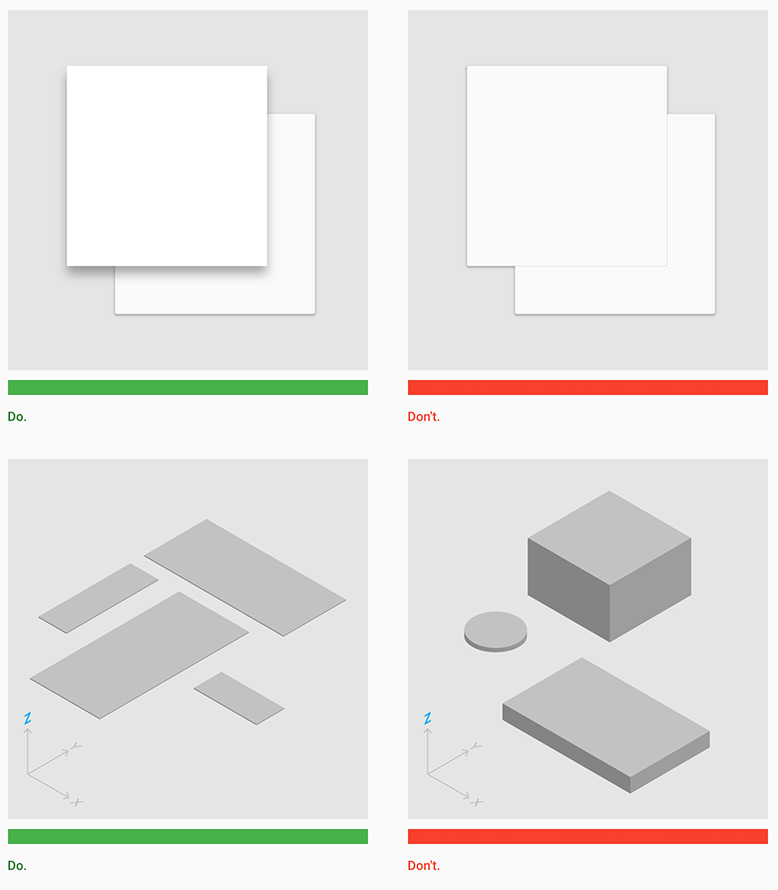
\includegraphics[width=0.5\textwidth]{fig/ainf/material-design-rules.png}
\caption{Material-Design}
\label{rpiAndDisplay}
\end{figure}
Mithilfe dieser Hintergrundinformation steht jetzt der Erstellung der grafischen Oberfläche nichts mehr im Weg.
\subsection{Umsetzung}
In diesem Kaptitel soll gezeigt werden, wie die grafische Oberfläche organisiert ist und wie diese mit den jeweiligen Controllern zusammenarbeitet.
Beschrieben werden jedoch nur wichtige Programmelemente und keine Grundlagen von JavaFX da dies ansonsten den Rahmen sprengen würde.\\
Realisiert wurde die Oberfläche mithilfe von 2 verschiedenen Fenstern auf welche anschließend in den Kapiteln \refname{sssec:startupController} und \refname{sssec:mainController} eingegangen wird.
\subsubsection{MVC-Implementierung}\label{sssec:mvc}
Wie schon in der Beschreibung von JavaFX erwähnt, organisiert sich die grafische Oberfläche nach dem MVC-Designpattern.
\subsubsection{Startup-Window und Controller}\label{sssec:startupController}
Aufgabe des Startup-Windows ist es, den Benutzer das Spiel, welches er spielen möchte, parametrisieren zu lassen.
Diese Parametrisierung beinhaltet das Auswählen eines Spielmodis sowie die Konfiguration der Spielernamen.\\\\
Die Auswahl eines Spielmodis erfolg über eine eigens dafür bereitgestellte ComboBox.
In dieser ComboBox befinden sich Objekte vom Typ \lstinline[style=java]{GamemodeModel}
\lstinputlisting[firstline=7, lastline=16, style=java,caption=fdsa,label=fdsafdsa]{src/data/model/GamemodeModel.java}
Sollte nun der Spieler nicht zufrieden mit gegebenen Spielmodis aus der ComboBox sein, kann er diese selbst auf ihn abstimmen und konfigurieren.
Es kann hier über das Interaktionsmenü die Karten-, Spieler-, und Automatic-Deal-Anzahl (AutoDeal) eingestellt werden.
Auch kann der Name des Spielmodis verändert werden.
Ist dies der Fall, führt das zu einer Ergänzung eines neuen Spielmodis mit den eingestellten Parametern in der eigens dafür vorgesehenen Konfigurationsdatei.\\\\
Auch ist, wie oben schon erwähnt, die Möglichkeit gegeben, Spielernamen zu bearbeiten.
Dies wird durch die Liste in \autoref{startupWindow} ersichtlich.
Wird in dieser Liste ein Spielernamen selektiert, übernimmt das Programm diesen direkt in das darüber befindliche Textfeld.
Von dort aus kann der Name bearbeitet werden.\\
Umgesetzt wird dies mithilfe von 2 sogenannte \lstinline[style=java]{ChangeListeners}, welche dauerhaft auf eine Veränderung, also einen "Change" warten um dann eine Methode auszuführen.
Neben Listener wären auch Properties und Bindings für diese Anwendung möglich.
Besser sind jedoch Listener.
\lstinputlisting[firstline=54, lastline=59, style=java,caption=fdsa,label=fdsafdsa]{src/gui/controller/StartupController.java}
So sind nun alle Preferenzen der Spieler gedeckt.\\\\
Folgend wird auf eine Besonderheit bei der Füllung der ComboBox und der Liste eingegangen.
Die Daten werden ab jetzt nicht mehr in der standard Darstellung angezeigt, sondern basiert auf einem eigens dafür angepassten Rendering.
Solch ein Verfahren hat den Vorteil, das nun direkt ein Objekt in die ComboBox bzw. in die Liste importiert werden kann und ab diesem Zeitpunk die Referenzierung des selektierten Elements leichter fällt.
Auch werden hierberi Resourcen eingespart, denn es werden nur die Elemente gerendert, die auch wirklich angezeigt werden.
Im \autoref{CellFactory} wird im ersten Schritt die Darstellung einer einzelnen Zelle definiert.
\lstinputlisting[firstline=302, lastline=313, style=java,caption=fdsa,label=CellFactory]{src/gui/controller/StartupController.java}
Jetzt muss ledeglich die CellFactory mithilfe des Methodenaufrufs \lstinline[style=java]{playerNameList.setCellFactory(list -> new PlayerCell())} gesetzt werden und die Liste baut sich nach dem import der Daten zusammen.
Genau das gleiche Verfahren kann auch bei der ComboBox angewendet werden.
\begin{figure}[H]
\centering
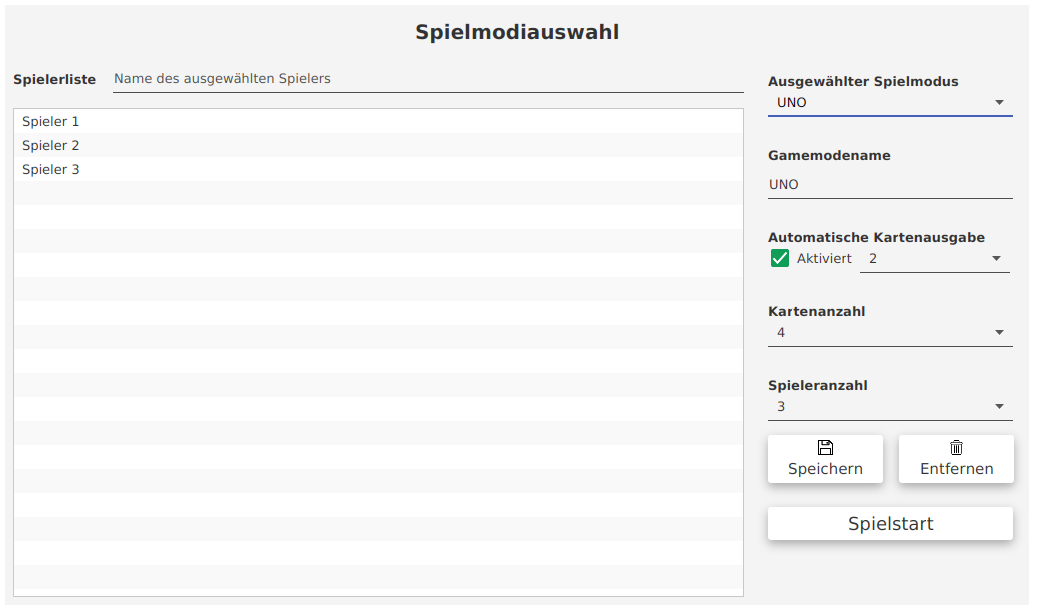
\includegraphics[width=0.8\textwidth]{fig/ainf/Startup_German.png}
\caption{Startup-Window}
\label{startupWindow}
\end{figure}
\subsubsection{Main-Window und Controller}\label{sssec:mainController}
\begin{figure}[H]
\centering
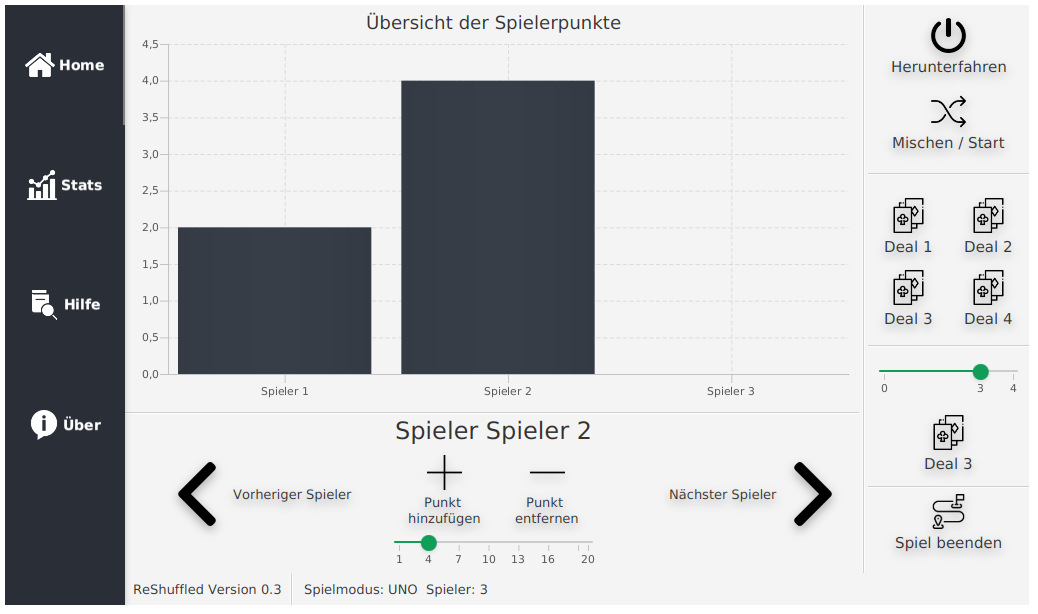
\includegraphics[width=0.8\textwidth]{fig/ainf/Main_Home_German.png}
\caption{Main-Window}
\label{mainWindows}
\end{figure}
\subsubsection{Home-Tab und Controller}
\subsubsection{Stats-Tab und Controller}\label{sssec:statsController}
\subsubsection{About- und Help-Tab und Controllers}
\subsection{Utility Klassen}
\subsubsection{AlertUtil}
\subsubsection{GuiUtil}
\subsection{Implementierung von CSS}
\subsection{Internationalisierung}
\subsubsection{Konzept}
\subsubsection{Umsetzung}
\subsubsection{Bereitstellung von Ressource-Bundles}

\section{Hardwarenahe-Programmierung}
\subsection{Einrichtung des Mikrocontrollers}
\subsection{Konzept und Ablaufdiagramm zur Kartenausgabe} \label{ssec:konzeptCardDeal}
\section{Teilaufbau}
\subsection{Raspberry PI}
\subsection{Raspberry PI Monitor}
\subsection{Montage und Testaufbau}\newpage
\begin{figure}[H]
\centering
\includegraphics[width=0.8\textwidth]{fig/ainf/IMG_3107.jpg}
\caption{Teilaufbau - Nicht bestromt}
\label{rpiAndDisplay}
\end{figure}
\subsection{Konfiguration des Zielsytsems}
\subsubsection{Betriebssystem}
\subsubsection{Integration des Touchpanels}
\subsubsection{Kommunikation über SSH}
\subsubsection{Autostart realisiert durch Services}

\section{Probleme - Verbesserungsmöglichkeiten - Zusammenfassung}
\subsection{Probleme}
\subsubsection{Probleme bei der Implementierung von JavaFX}
\subsubsection{Kommunikation zwischen Controllern}
\subsection{Verbesserungsmöglichkeiten}
\subsubsection{Online Update-Möglichkeit der Software}
\subsubsection{Smartphone-Interface zum Zählen der Punkte}
\subsection{Zusammenfassung}
    \lohead{Alle}
    \chapter{Gesamtsystemtests}


    

\renewcommand\appendixname{Anhang}
\renewcommand\appendixpagename{Anhang}
\renewcommand\appendixtocname{Anhang}

\lohead{}

% Anhang Seite ohne Kopf- & Fußzeile
\appendix
\begingroup
\makeatletter
\let\ps@plain\ps@empty
\appendixpage
\makeatother
\endgroup

% Anhänge
\chapter{Zeitaufzeichnung}
\chapter{Persönlicher Anhang 1}

\markboth{}{}	%end chapter

\printbibliography
\nocite{*}

\chapter{Abkürzungsverzeichnis}
\begin{acronym}
	%Abkürzung hinzufügen: \acro{Kürzel}{Ausgeschrieben}
	\acro{WLAN}{Wireless Local Area Network}
	\acro{WWW}{World Wide Web}
	\acro{uC}[µC]{Mikrocontroller}
\end{acronym}

\listoffigures
\listoftables
\lstlistoflistings
\end{document}
